\documentclass[12pt,a4paper]{article}

% --- Pacotes de Suporte ---
\usepackage{cmap} % corrige o mapeamento Unicode de ligaduras (fi/ff/fl) na
                   % extracao de texto do PDF -- deve vir antes de fontenc
\usepackage[utf8]{inputenc}
\usepackage[T1]{fontenc}
\usepackage[expansion=false]{microtype}
\usepackage[brazilian]{babel}
\usepackage{amsmath}
\usepackage{amsfonts}
\usepackage{amssymb}
\usepackage{geometry}
\usepackage{bm}
\usepackage{graphicx}
\usepackage{float}
\usepackage{booktabs}
\usepackage{hyperref}
\usepackage{fancyhdr}
\usepackage{titlesec}
\usepackage{tabularx}
\usepackage{longtable}

% Termos técnicos em inglês e acrônimos: o babel-brazilian aplica padrões de
% hifenização do português a eles, produzindo quebras erradas (ex.: "Offloa-ding",
% "ASH-RAE"). A lista abaixo dá o padrão correto de cada termo recorrente; os
% acrônimos entram sem nenhum ponto de quebra, para nunca serem partidos.
\hyphenation{
  off-shore Off-shore off-load-ing Off-load-ing
  head-er blow-down blow-hole load shed-ding
  sur-ro-gate foul-ing rub-bing tim-ing
  Auto-en-coder auto-en-coder En-gi-neer-ing en-gi-neer-ing
  Non-lin-ear non-lin-ear
  ASHRAE NORSOK AGMA NEMA API ISO IEC ASME EKF VAE PIML PINN MPC PSO
  PSA VSD VFD SPC LMTD NTU RUL SHAP GUM MHE FNO
}

\numberwithin{equation}{section}
\numberwithin{table}{section}
\numberwithin{figure}{section}

\geometry{margin=2.5cm, headheight=15pt}
\addtolength{\topmargin}{-0.5pt}
\setlength{\emergencystretch}{1em}

\hypersetup{
	colorlinks=true,
	linkcolor=black,
	citecolor=black,
	urlcolor=black,
	pdftitle={Gêmeo Digital de Sistemas de Compressão Offshore},
	pdfauthor={Marcelo Moreira Mejias},
	pdfsubject={Diretrizes Técnicas, Modelagem e Implementação},
	pdfkeywords={compressor de parafuso, offshore, gêmeo digital, PIML, EKF, MPC}
}

\pagestyle{fancy}
\fancyhf{}
\renewcommand{\sectionmark}[1]{\markboth{#1}{}}
\fancyhead[L]{\nouppercase{\leftmark}}
\fancyhead[R]{\thepage}
\renewcommand{\headrulewidth}{0.4pt}

% --- Identificação de volume/revisão (coleção versionada, ver CONTEXTO.md) ---
\newcommand{\colecaotitulo}{Enciclopédia de Máquinas Rotodinâmicas}
\newcommand{\volumeatual}{Volume I}
\newcommand{\revdata}{Rev. 26/07/2026}

% --- Identidade visual dos capítulos (\section = capítulo nesta classe article) ---
\newcommand{\chapterword}{Capítulo}
\titleformat{\section}
	{\normalfont\Large\bfseries\raggedright}
	{\chapterword~\thesection}{1em}{}
	[\vspace{-0.5em}\rule{\textwidth}{0.4pt}]


\begin{document}


	% --- Definições de Título e Autoria ---
	%\title{\textbf{Diretriz Técnica: Implementação de Gêmeo Digital (Digital %Twin) para Sistemas de Compressão e Armazenamento de Ar Offshore}}
	%\author{\textbf{Engenheiro Marcelo Moreira Mejias, M.Sc.}}
	%\date{}
	
	% --- CAPA ---
	\begin{titlepage}
		\centering
		\vspace*{1.5cm}
		{\large \textsc{\colecaotitulo\ --- \volumeatual}} \\[1cm]
		\rule{\textwidth}{0.4pt} \\[0.8cm]
		{\Huge \textbf{Gêmeo Digital de Sistemas de Compressão Offshore}} \\[0.5cm]
		{\Large \textbf{Diretrizes Técnicas, Modelagem e Implementação}} \\[0.8cm]
		\rule{\textwidth}{0.4pt} \\[1.5cm]

		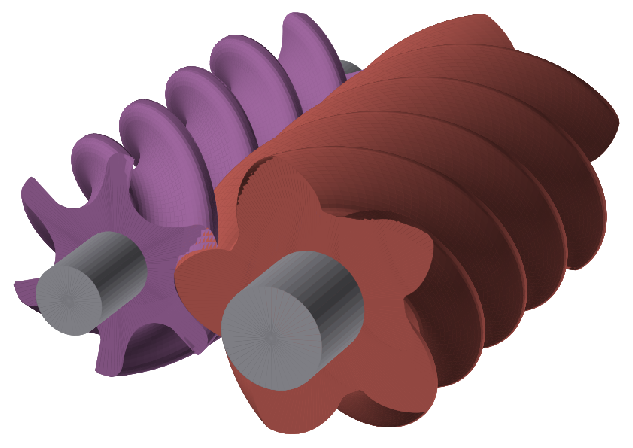
\includegraphics[width=0.42\textwidth]{figuras/fig_3_1_parafuso3d.pdf} \\[1.5cm]

		\vfill
		{\large \textbf{Autor: Engenheiro Marcelo Moreira Mejias, M.Sc.}} \\[0.5cm]

		{\large \today} \\[0.3cm]
		{\normalsize \revdata}
	\end{titlepage}
	
	% --- DEDICATÓRIA ---
	\newpage
	\thispagestyle{empty}
	\vspace*{\fill}
	\begin{flushright}
		\textit{Este trabalho foi criado para as futuras gerações da empresa e que já devem achar isso muito arcaico agora ou em poucos anos.}
	\end{flushright}
	\vspace*{\fill}
	

% --- PREFÁCIO ---
\newpage
\section*{Prefácio}
\addcontentsline{toc}{section}{Prefácio}

O ar comprimido é, para a maioria das plantas industriais, uma utilidade tão presente que raramente recebe a atenção técnica dedicada a sistemas mais visíveis, como geração de energia ou processamento principal. Em unidades de produção offshore — FPSOs, plataformas fixas e semissubmersíveis — essa relação de importância se inverte. Ali, o ar comprimido deixa de ser coadjuvante: alimenta a instrumentação pneumática, as válvulas de segurança e os sistemas de parada de emergência (ESD), e sua indisponibilidade pode comprometer diretamente a integridade operacional da unidade. Nesse ambiente — onde o acesso é restrito, o custo de uma parada não programada é elevado e as condições de salinidade, umidade e espaço são adversas ao equipamento — o compressor de parafuso rotativo se consolidou como a máquina de escolha para geração contínua de ar de processo e de instrumentação, exatamente por unir robustez, deslocamento positivo estável e compatibilidade com operação isenta de óleo.

Este livro nasceu da constatação de que, apesar de sua centralidade, o compressor de parafuso raramente é tratado como um sistema integrado. A literatura técnica tende a fragmentar o assunto entre manuais de fabricante, normas isoladas e conhecimento tácito de manutenção — cada um cobrindo uma fatia do problema, poucos conectando a física da máquina ao seu comportamento de falha e, menos ainda, à possibilidade de antecipar essas falhas com dados. A proposta aqui é diferente: construir, capítulo a capítulo, uma modelagem completa e conectada — do princípio físico de funcionamento do rotor helicoidal até um Gêmeo Digital funcional, capaz de aprender, prever e prescrever.

O percurso do livro segue essa lógica de construção progressiva. Começamos pela justificativa de uso do compressor de parafuso na indústria em geral e, com foco particular, no ambiente offshore de petróleo e gás — os desafios de salinidade, umidade relativa elevada, atmosferas explosivas e redes elétricas isoladas que tornam esse ambiente distinto de uma planta terrestre convencional. A partir daí, desmontamos o conjunto compressor peça por peça: os rotores e seu perfil geométrico, o trem de potência e a caixa multiplicadora, o motor elétrico e o inversor de frequência, os sistemas de lubrificação, resfriamento, filtragem e secagem, e os vasos de armazenamento e distribuição. Cada componente é tratado sob três lentes simultâneas — o elemento de máquina em si (sua função e seus acessórios), a modelagem termodinâmica e mecânica que rege seu comportamento, e os mecanismos de falha que podem degradá-lo — porque um Gêmeo Digital que não sabe \textit{como} um componente falha não consegue preveni-la.

A segunda metade do livro eleva esse equacionamento disperso a um modelo unificado. Ali se apresenta a metodologia de construção do motor de cálculo do Gêmeo Digital: como as equações de primeiros princípios de cada capítulo anterior se conectam em um único sistema de estimação de estado (via Filtro de Kalman Estendido), como a alta dimensionalidade dos dados de campo é reduzida sem perda de informação crítica (via Autoencoder Variacional), como o conhecimento físico é injetado diretamente no aprendizado de máquina para garantir que nenhuma predição viole as leis da termodinâmica (Physics-Informed Machine Learning), e como tudo isso se traduz em decisões operacionais concretas através de controle preditivo e otimização (MPC e PSO).

O objetivo final não é acadêmico — é prático e mensurável. Um Gêmeo Digital construído sobre essa base permite operar o trem de compressão mais próximo do limite termodinâmico real da máquina, reduzindo o consumo específico de energia; quantificar, em unidades comparáveis, onde a eficiência está sendo destruída por irreversibilidades, reduzindo por consequência direta a geração de CO\textsubscript{2} equivalente; e substituir a manutenção por calendário por uma manutenção baseada em condição real, antecipando falhas antes que se tornem paradas não programadas. Estas três metas — menor consumo energético, menor pegada de carbono e manutenção preditiva — não são objetivos independentes neste livro: são consequências naturais de um único modelo bem construído.

Este é, portanto, um livro para ser lido de duas formas. Como referência técnica, cada capítulo é autocontido o suficiente para ser consultado isoladamente diante de um problema específico de campo. Como metodologia, ele é sequencial: a compreensão de um Gêmeo Digital completo exige percorrer o caminho do princípio físico até a inteligência artificial, sem atalhos, porque é exatamente essa conexão — física restritiva, dados confiáveis e algoritmos explicáveis — que diferencia um verdadeiro Gêmeo Digital de um simples painel de sensores.

\vspace{1em}
\hfill \textit{O Autor}

	% --- SUMÁRIO ---
	\newpage
	\tableofcontents
	\newpage

	% --- LISTAS DE FIGURAS E TABELAS ---
	% Obra de consulta: o leitor frequentemente procura uma figura ou matriz de
	% falhas específica sem saber em que capítulo ela está. Ambas entram no
	% sumário via \addcontentsline.
	\phantomsection
	\addcontentsline{toc}{section}{Lista de Figuras}
	\listoffigures
	\newpage
	\phantomsection
	\addcontentsline{toc}{section}{Lista de Tabelas}
	\listoftables
	\newpage

% --- NOMENCLATURA ---
\newpage
\section*{Nomenclatura}
\addcontentsline{toc}{section}{Nomenclatura}

A tabela abaixo reúne os símbolos empregados neste documento, seu significado, unidade típica (SI) e o(s) capítulo(s) onde aparecem. Símbolos com subscrito próprio (ex.: $P_{HP,\text{out}}$, $T_{w,\text{in}}$) não são listados individualmente — apenas a base do símbolo é definida aqui, e o subscrito segue a convenção descrita junto a cada equação. Onde duas grandezas diferentes disputavam a mesma letra em versões anteriores deste documento, o símbolo de uso menos frequente foi renomeado (com subscrito ou letra alternativa) para que cada símbolo tenha um único significado em todo o texto — essas escolhas estão marcadas com \dag.

{\small
\setlength{\tabcolsep}{3pt}
\renewcommand{\arraystretch}{1.15}

\subsection*{Constantes e Grandezas Termodinâmicas Gerais}
\begin{longtable}{>{\raggedright\arraybackslash}p{2.8cm} >{\raggedright\arraybackslash}p{5.3cm} >{\raggedright\arraybackslash}p{2.1cm} >{\raggedright\arraybackslash}p{4.2cm}}
	\toprule
	\textbf{Símbolo} & \textbf{Significado} & \textbf{Unidade} & \textbf{Capítulos} \\ \midrule
	\endhead
	$P$ & Pressão & Pa, bar & Todos \\
	$T$ & Temperatura & K, $^{\circ}$C & Todos \\
	$\rho$ & Massa específica (densidade) & kg\,m$^{-3}$ & Termofluídica \\
	$v$ & Velocidade do escoamento & m\,s$^{-1}$ & Perda de carga, filtros \\
	$\dot{m}$ & Vazão mássica & kg\,s$^{-1}$ & Todos \\
	$\dot{V}$ & Vazão volumétrica & m$^3$\,s$^{-1}$ & Todos \\
	$\dot{V}_{\text{free\_air}}$ & Vazão convertida às condições de referência de admissão (FAD, \textit{Free Air Delivery}), ISO 1217 & m$^3$\,s$^{-1}$ & Cap. 11, 16 \\
	$\dot{W}$ & Potência (trabalho por unidade de tempo) & W, kW & Todos \\
	$\dot{Q}$ & Taxa de transferência de calor & W & Trocadores, Cap. 2, 9 \\
	$n$ & Índice politrópico do processo de compressão & adimensional & Cap. 5, 9, 11 \\
	$R$ & Constante do gás (ar) & J\,kg$^{-1}$\,K$^{-1}$ & Todos \\
	$\gamma$ & Razão de calores específicos ($c_p/c_v$) do ar & adimensional ($\approx 1.4$) & Termofluídica \\
	$c_p$ & Calor específico a pressão constante & J\,kg$^{-1}$\,K$^{-1}$ & Termofluídica \\
	$\eta$ & Eficiência (com subscrito indicando qual: $\eta_{vol}$, $\eta_{is}$, $\eta_{mec}$, etc.) & adimensional & Todos \\
	$\eta_p$ & Eficiência politrópica (aproximadamente constante ao longo do mapa de operação) & adimensional & Cap. 9 \\
	$\Pi$ & Razão de pressão do estágio ($P_2/P_1$) & adimensional & Cap. 9, 11 \\
	$f_D$\dag & Fator de atrito de Darcy (perda de carga distribuída em tubulação) & adimensional & Cap. 5 \\
	$L_{\text{linha}}$ & Comprimento do trecho de tubulação interestágios & m & Cap. 5 \\
	$D_{\text{linha}}$ & Diâmetro interno do trecho de tubulação interestágios & m & Cap. 5 \\
	$\omega$ & Velocidade angular do rotor/eixo & rad\,s$^{-1}$ & Todos \\ \bottomrule
\end{longtable}

\subsection*{Geometria e Física do Compressor de Parafuso}
\begin{longtable}{>{\raggedright\arraybackslash}p{2.8cm} >{\raggedright\arraybackslash}p{5.3cm} >{\raggedright\arraybackslash}p{2.1cm} >{\raggedright\arraybackslash}p{4.2cm}}
	\toprule
	\textbf{Símbolo} & \textbf{Significado} & \textbf{Unidade} & \textbf{Capítulos} \\ \midrule
	\endhead
	$V_i$ & Razão volumétrica interna do rotor ($V_1/V_2$), fixa por projeto & adimensional & Cap. 5 \\
	$\pi_i$ & Razão de pressão interna ideal ($V_i^{\,n}$) & adimensional & Cap. 5 \\
	$V_{\text{disp}}$ & Volume deslocado pelo rotor por rotação (definido pela geometria do perfil helicoidal) & m$^3$ & Cap. 3, 13 \\
	$\delta$ & Folga radial ou de flanco entre rotores/carcaça & m, $\mu$m & Cap. 9, 11 \\
	$A_{\text{leak}}$ & Área de fuga total entre câmaras de pressões distintas & m$^2$ & Cap. 9 \\
	$Z$ & Número de lóbulos/dentes (sempre com subscrito: $Z_{\text{bull}}$, $Z_{\text{macho}}$, etc.) & adimensional & Cap. 6, 8, 9 \\
	$GMF$ & Frequência de engrenamento (\textit{Gear Mesh Frequency}) & Hz & Cap. 6, 8 \\
	$f_{bp}$ & Frequência de passagem dos lóbulos & Hz & Cap. 9, header \\
	$D_{\text{macho}}$ & Diâmetro externo do rotor macho & m & Cap. 9 \\
	$u_{\text{tip}}$ & Velocidade periférica (tangencial) da ponta do rotor macho & m\,s$^{-1}$ & Cap. 9 \\
	$M_{\text{tip}}$ & Número de Mach na ponta do rotor & adimensional & Cap. 9 \\
	$M_c$ & Massa térmica (capacidade calorífica) da carcaça do elemento LP & kg & Cap. 9 \\
	$c_c$ & Calor específico do material da carcaça & J\,kg$^{-1}$\,K$^{-1}$ & Cap. 9 \\
	$G_{\text{ext}}$\dag & Condutância térmica de convecção natural da carcaça para o ambiente & W\,K$^{-1}$ & Cap. 9 \\
	$G_{\text{arref}}$\dag & Condutância térmica do arrefecimento ativo/ventilação forçada do invólucro & W\,K$^{-1}$ & Cap. 9 \\
	$\tau_c$\dag & Constante de tempo térmica da carcaça (mesma família de $\tau_{th}$/$\tau_{bd}$, distinta do torque $\tau$) & s & Cap. 9 \\ \bottomrule
\end{longtable}

\subsection*{Controle, Modulação e Válvulas}
\begin{longtable}{>{\raggedright\arraybackslash}p{2.8cm} >{\raggedright\arraybackslash}p{5.3cm} >{\raggedright\arraybackslash}p{2.1cm} >{\raggedright\arraybackslash}p{4.2cm}}
	\toprule
	\textbf{Símbolo} & \textbf{Significado} & \textbf{Unidade} & \textbf{Capítulos} \\ \midrule
	\endhead
	$C_d$ & Coeficiente de descarga do orifício (razão entre a vazão real e a isentrópica ideal) & adimensional & Cap. 11, 13, 14 \\
	$A_v$ & Área efetiva de passagem da válvula de admissão & m$^2$ & Cap. 13 \\
	$\Phi(r)$ & Função de escoamento compressível em orifício, com os regimes subsônico e bloqueado & adimensional & Cap. 13, 14 \\
	$r$, $r_{cr}$ & Razão de pressões através da válvula e seu valor crítico de bloqueio sônico ($\approx 0{,}528$ para o ar) & adimensional & Cap. 13 \\
	$\tau_{bd}$\dag & Constante de tempo do \textit{blow-down} (o subscrito evita colisão com o torque $\tau$) & s & Cap. 13 \\
	$\bar{f}$ & Frequência normalizada do inversor ($f/f_{\text{nom}}$) & adimensional & Cap. 13 \\
	$x_c$\dag & Fração da capacidade nominal demandada pela planta (o subscrito distingue do vetor de estado $x$ do EKF) & adimensional & Cap. 13 \\
	$k_{ul}$ & Fração da potência nominal ainda consumida em alívio (\textit{unload}) & adimensional & Cap. 13 \\
	$\eta_{vsd}$ & Rendimento combinado de motor e inversor em carga parcial & adimensional & Cap. 13 \\
	$\Delta P_{db}$ & Banda morta de pressão entre corte e religamento & bar & Cap. 13 \\
	$f_{\text{ciclo}}$ & Frequência de ciclagem carga/alívio & h$^{-1}$ & Cap. 13 \\
	$E_{\Pi}$ & Elasticidade da potência de compressão em relação à razão de pressão & adimensional & Cap. 13 \\
	$\delta$ (contexto de controle)\dag & Estado binário da válvula de admissão (1 = carga, 0 = alívio) — distinto da folga $\delta$ dos capítulos de rotores & adimensional & Cap. 13 \\
	$C_{op}$ & Custo operacional acumulado do ciclo carga/alívio & R\$, kWh & Cap. 13 \\
	$\zeta_{\text{valv}}$\dag & Coeficiente de perda de carga localizada de válvulas de alívio/retenção (\textit{blow-off}, \textit{check}, PSV) — mesma família de $\zeta$ do filtro (Cap. 5), com subscrito próprio & adimensional & Cap. 5, 28 \\ \bottomrule
\end{longtable}

\subsection*{Elétrica e Acionamento}
\begin{longtable}{>{\raggedright\arraybackslash}p{2.8cm} >{\raggedright\arraybackslash}p{5.3cm} >{\raggedright\arraybackslash}p{2.1cm} >{\raggedright\arraybackslash}p{4.2cm}}
	\toprule
	\textbf{Símbolo} & \textbf{Significado} & \textbf{Unidade} & \textbf{Capítulos} \\ \midrule
	\endhead
	$I$ & Corrente elétrica & A & Cap. 4 \\
	$V_L$ & Tensão de linha & V & Cap. 4, 19 \\
	$f$ & Frequência elétrica de alimentação/VSD & Hz & Cap. 4 \\
	$s$ & Escorregamento do motor de indução & adimensional & Cap. 4 \\
	$N_{mot}$\dag & Rotação medida do motor (RPM) & RPM & Cap. 4, 6, 8 \\
	$p$ & Número de polos do motor & adimensional & Cap. 4 \\
	$\tau$ & Torque (sempre com subscrito indicando o eixo/componente) & N\,m & Cap. 4, 6, 8 \\
	$\text{THD}_i$ & Distorção harmônica total de corrente & \% & Cap. 3, 4 \\
	$j$\dag & Ordem do harmônico na equação de bandas laterais & adimensional & Cap. 4 \\
	$k_{\text{relé}}$\dag & Constante da curva de disparo do relé (IEC 60255) & adimensional & Cap. 4 \\
	$VU$ & Desbalanço de tensão entre fases (NEMA MG1) & \% & Cap. 4 \\
	$IU$ & Desbalanço de corrente entre fases (NEMA MG1) & \% & Cap. 4 \\
	$\Delta T_{\text{fases}}$ & Espalhamento entre as três temperaturas de enrolamento por fase & K, $^{\circ}$C & Cap. 4 \\
	$P_{ag}$ & Potência elétrica que atravessa o entreferro do motor ($\tau_{em}\cdot\omega_s$) & W & Cap. 4 \\
	$P_{\text{fixas}}$ & Perdas do motor pouco sensíveis à carga (estator, núcleo, atrito/ventilação, suplementares), de ensaio & W & Cap. 4 \\ \bottomrule
\end{longtable}

\subsection*{Vibração, Fadiga e Rotordinâmica}
\begin{longtable}{>{\raggedright\arraybackslash}p{2.8cm} >{\raggedright\arraybackslash}p{5.3cm} >{\raggedright\arraybackslash}p{2.1cm} >{\raggedright\arraybackslash}p{4.2cm}}
	\toprule
	\textbf{Símbolo} & \textbf{Significado} & \textbf{Unidade} & \textbf{Capítulos} \\ \midrule
	\endhead
	$\sigma_b$ & Tensão de flexão na raiz do dente (modelo de Lewis) & MPa & Cap. 8, 19, 20 \\
	$b$ & Largura de face do dente da engrenagem (equação de Lewis) & mm & Cap. 8 \\
	$b_f$\dag & Expoente da curva S-N de Basquin (Regra de Miner) & adimensional & Cap. 20 \\
	$D$ & Dano acumulado por fadiga (Regra de Palmgren-Miner), $D=1$ na falha & adimensional & Cap. 20 \\
	$L_{10h}$ & Vida nominal do rolamento com 90\% de confiabilidade & horas & Cap. 8, 11 \\
	$N_{\text{rot}}$\dag & Rotação do eixo do rolamento — sempre em RPM nas equações de vida $L_{10h}$, onde o fator 60 do denominador faz a conversão para horas & RPM & Cap. 8, 11 \\
	$\omega_{cr}$ & Velocidade crítica (rotordinâmica) & rad\,s$^{-1}$ & Cap. 8 \\
	$v_{\text{rms}}$ & Severidade de vibração global (valor eficaz de velocidade, banda larga) & mm\,s$^{-1}$ & Cap. 18, 19 \\
	$v_{\text{trip}}$ & Limiar de vibração para desligamento (ESD), específico da máquina — critério de API 619/OEM ou linha de base de comissionamento, não valor tabelado & mm\,s$^{-1}$ & Cap. 18 \\
	$\delta_{ax}$ & Posição axial do rotor HP, medida por sonda de proximidade no mancal de escora (deriva por desgaste do rolamento, precede a vibração) & $\mu$m & Cap. 11, 18 \\ \bottomrule
\end{longtable}

\subsection*{Psicrometria e Trocadores de Calor}
\begin{longtable}{>{\raggedright\arraybackslash}p{2.8cm} >{\raggedright\arraybackslash}p{5.3cm} >{\raggedright\arraybackslash}p{2.1cm} >{\raggedright\arraybackslash}p{4.2cm}}
	\toprule
	\textbf{Símbolo} & \textbf{Significado} & \textbf{Unidade} & \textbf{Capítulos} \\ \midrule
	\endhead
	$U$ & Coeficiente global de transferência de calor & W\,m$^{-2}$\,K$^{-1}$ & Cap. 5, 10, 12, 14 \\
	$A$ & Área de troca térmica & m$^2$ & Cap. 5, 10, 14 \\
	$\Delta T_{lm}$ (LMTD) & Diferença de temperatura média logarítmica & K & Cap. 10, 12, 14 \\
	$\epsilon$ & Efetividade do trocador de calor & adimensional & Cap. 7, 10, 12, 14 \\
	$R_f$ & Resistência térmica adicional por incrustação (\textit{fouling}) & m$^2$\,K\,W$^{-1}$ & Cap. 10 \\
	$UA$ & Condutância térmica global do trocador (produto $U \cdot A$), invariante às temperaturas de entrada & W\,K$^{-1}$ & Cap. 12 \\
	$NTU$ & Número de unidades de transferência, $UA/C_{\min}$ & adimensional & Cap. 12 \\
	$C_{\min}, C_{\max}, C_r$ & Capacidades térmicas ($\dot{m}\,c_p$) menor e maior entre as duas correntes, e sua razão $C_{\min}/C_{\max}$ & W\,K$^{-1}$; adimensional & Cap. 12 \\
	$\eta_{UA}$ & Fator de degradação do resfriador, $UA_{\text{real}}/UA_{\text{projeto}}$ & adimensional & Cap. 12 \\
	$a_{tv}$\dag & Fração da vazão de óleo enviada ao resfriador pela válvula termostática de três vias (o subscrito evita colisão com a constante $a$ da curva de Vogel) & adimensional & Cap. 12 \\
	$\tau_{th}$\dag & Constante de tempo térmica do circuito de óleo (o subscrito evita colisão com o torque $\tau$) & s & Cap. 12 \\
	$M_{\text{óleo}}$ & Massa de óleo do circuito (reservatório e tubulação) & kg & Cap. 12 \\
	$W$\dag & Razão de umidade (kg água / kg ar seco) — notação ASHRAE & adimensional & Cap. 10, 14 \\
	$\phi$ & Umidade relativa & \%, adimensional & Cap. 10 \\
	$P_{\text{sat}}(T)$ & Pressão de saturação do vapor d'água na temperatura $T$ & kPa & Cap. 10 \\
	$T_{dp}$ & Ponto de orvalho sob pressão & $^{\circ}$C & Cap. 3, 14, 15, 19 \\
	$e_{\text{filme}}$\dag & Espessura do filme de óleo no mancal & m, $\mu$m & Cap. 7 \\
	$k_{ads}$\dag & Constante de taxa de adsorção do dessecante & s$^{-1}$ & Cap. 14 \\
	$\dot{Q}_{\text{gerado}}$ & Calor total gerado dentro do invólucro do pacote (motor, VSD, gearbox, casco) & W & Cap. 2 \\
	$\dot{Q}_{\text{hood}}$ & Calor removido pelo exaustor forçado do invólucro & W & Cap. 2, 14 \\
	$\dot{m}_{\text{vent}}$ & Vazão mássica de ar de ventilação forçada do invólucro & kg\,s$^{-1}$ & Cap. 2 \\
	$\eta_{purge}$ & Fração da vazão total não perdida como ar de purga de regeneração & adimensional & Cap. 14 \\
	$\dot{Q}_{\text{disp}}$ & Calor residual disponível para recuperação (aftercooler + óleo + hood) & W & Cap. 14 \\
	$\epsilon_{\text{recup}}$ & Efetividade do trocador de recuperação de calor para regeneração & adimensional & Cap. 14 \\ \bottomrule
\end{longtable}

\subsection*{Exergia e Sustentabilidade}
\begin{longtable}{>{\raggedright\arraybackslash}p{2.8cm} >{\raggedright\arraybackslash}p{5.3cm} >{\raggedright\arraybackslash}p{2.1cm} >{\raggedright\arraybackslash}p{4.2cm}}
	\toprule
	\textbf{Símbolo} & \textbf{Significado} & \textbf{Unidade} & \textbf{Capítulos} \\ \midrule
	\endhead
	$\dot{I}$ & Taxa de destruição de exergia (irreversibilidade) & W & Cap. 15, 19 \\
	$\psi$\dag & Exergia específica de fluxo (notação de Kotas) & J\,kg$^{-1}$ & Cap. 15, 19 \\
	$\eta_{ex}$ & Eficiência exergética global & adimensional & Cap. 15, 19 \\
	$T_0$ & Temperatura do ambiente de referência (morto termodinâmico) & K & Cap. 15, 19 \\
	$\dot{S}_{gen}$ & Taxa de geração de entropia & W\,K$^{-1}$ & Cap. 15, 19 \\
	$h$ & Entalpia específica & J\,kg$^{-1}$ & Cap. 15, 19 \\
	$s$ (contexto exergético) & Entropia específica & J\,kg$^{-1}$\,K$^{-1}$ & Cap. 15, 19 \\
	$N_{\text{frota}}$\dag & Número de compressores ativos na frota (somatórios) & adimensional & Cap. 14 \\ \bottomrule
\end{longtable}

\subsection*{Estimação de Estado, IA e Otimização}
\begin{longtable}{>{\raggedright\arraybackslash}p{2.8cm} >{\raggedright\arraybackslash}p{5.3cm} >{\raggedright\arraybackslash}p{2.1cm} >{\raggedright\arraybackslash}p{4.2cm}}
	\toprule
	\textbf{Símbolo} & \textbf{Significado} & \textbf{Unidade} & \textbf{Capítulos} \\ \midrule
	\endhead
	$x$ & Vetor de estados do sistema (EKF) & --- & Cap. 20 \\
	$z$ & Vetor de medições/observações (EKF) ou variável genérica de entrada (VAE) & --- & Cap. 19, 20 \\
	$g$\dag & Função não linear de observação do EKF, $z=g(x)$ & --- & Cap. 20 \\
	$Q$ & Matriz de covariância do ruído de processo (EKF) & --- & Cap. 20 \\
	$\mathcal{R}$\dag & Matriz de covariância do ruído de \textbf{medição} (EKF) & --- & Cap. 20 \\
	$\kappa_{\text{port}}$\dag & Fator de inflação de $\mathcal{R}$ para leituras de sensor portátil/wireless ($\kappa$ está ocupado pelo fator de suavização do PIML) & --- & Cap. 18 \\
	$F_k, G_k$ & Jacobianas de transição de estado e de observação (EKF) & --- & Cap. 20 \\
	$\Lambda$ & Vetor de parâmetros estáticos calibráveis, aumentado ao estado do EKF & --- & Cap. 28 \\
	$Q_\Lambda$\dag & Covariância de processo dos parâmetros estáticos aumentados — próxima de zero na janela de calibração, pequena para acompanhar deriva lenta depois (distingue-se de $Q$, a covariância do estado dinâmico original) & --- & Cap. 28 \\
	$u$ & Vetor de entradas conhecidas (comandos ao VSD, demanda) & --- & Cap. 21 \\
	$n_x, n_z$\dag & Dimensões dos vetores de estado e de medição (subscritos evitam colisão com o índice politrópico $n$ e o módulo de engrenagem $m$) & --- & Cap. 21 \\
	$\mathcal{O}$ & Matriz de observabilidade do sistema linearizado & --- & Cap. 21 \\
	$\tilde{z}_k$ & Inovação: diferença entre medição e predição, $z_k - g(\hat{x}_{k|k-1})$ & --- & Cap. 21 \\
	$S_k$\dag & Covariância da inovação (o subscrito e a ausência de ponto distinguem da taxa de geração de entropia $\dot{S}_{gen}$) & --- & Cap. 21 \\
	$\text{NIS}_k$ & Inovação normalizada ao quadrado; estatística $\chi^2$ de validação do EKF & --- & Cap. 21 \\
	$\ell$\dag & Vetor do espaço latente (VAE) & --- & Cap. 15, 20 \\
	$E_{\text{rec}}$ & Erro de reconstrução (VAE), usado como resíduo de anomalia & --- & Cap. 15, 20 \\
	$\beta$ & Peso da divergência KL na perda do VAE & --- & Cap. 22 \\
	$d$ & Dimensão do espaço latente do VAE & --- & Cap. 22 \\
	$\tau_{\text{limiar}}$\dag & Limiar de disparo do erro de reconstrução (o subscrito evita colisão com o torque $\tau$) & --- & Cap. 18, 22 \\
	$\alpha$ & Taxa de falsos alarmes aceita no dimensionamento de $\tau_{\text{limiar}}$ & --- & Cap. 22 \\
	$d_M$ & Distância de Mahalanobis no espaço latente & --- & Cap. 22 \\
	$\mathcal{F}$ & Resíduo físico imposto à rede no PIML & --- & Cap. 20, 23 \\
	$\lambda$ & Peso da consistência física na perda do PIML & --- & Cap. 23 \\
	$N_f$ & Número de pontos de colocação (avaliação do resíduo físico) & --- & Cap. 23 \\
	$\kappa$ & Fator de suavização do balanceamento adaptativo de $\lambda$ & --- & Cap. 23 \\
	$\theta$\dag & Parâmetros treináveis da rede neural (distinto do ângulo de torção $\Delta\theta$ do Cap. 6) & --- & Cap. 23 \\
	$\Xi$ & Parâmetro físico desconhecido identificado por problema inverso (PINN), otimizado junto aos pesos da rede & --- & Cap. 23 \\
	$\rho$\dag & Peso do esforço de controle $\Delta u$ no MPC (distinto da massa específica $\rho$ dos capítulos de termofluídica) & --- & Cap. 24 \\
	$\varsigma$ & Variável de folga de restrição branda no MPC & --- & Cap. 24 \\
	$\varrho_s$ & Penalidade aplicada à variável de folga $\varsigma$ & --- & Cap. 24 \\
	$w$\dag & Peso de inércia do PSO (distinto do trabalho $W$ e do ruído de processo $w$ do EKF) & --- & Cap. 24 \\
	$c_1, c_2$ & Coeficientes cognitivo e social do PSO & --- & Cap. 24 \\
	$HI$ & \textit{Health Index}: índice agregado de saúde da máquina, de 0 a 1 & --- & Cap. 26 \\
	$\Theta_j$\dag & $j$-ésimo indicador componente do $HI$ ($\zeta$ está ocupado pelo coeficiente de perda de filtro) & --- & Cap. 26 \\
	$\varpi_j$\dag & Peso do indicador $j$ no $HI$ ($\omega$ está ocupado pela velocidade angular) & --- & Cap. 26 \\
	$J$ & Função de custo/objetivo (MPC, PSO) & --- & Cap. 15, 20 \\
	$H$ & Horizonte de predição (MPC) & passos & Cap. 15, 20 \\
	$k$ & Índice de tempo discreto (sempre como subscrito: $x_k$, $z_k$) & --- & Cap. 15, 20 \\
	$RUL$ & \textit{Remaining Useful Life} — vida útil remanescente projetada (base: dano acumulado, Eq. 19.9; com subscrito, projeção sobre outra variável de estado, ex. $RUL_\delta$ no Cap. 29) & tempo/ciclos & Cap. 19, 29 \\
	$\mathcal{M}$ & Subconjunto do catálogo de mecanismos de falha (Tabela~28.2) considerado na busca por resíduo mínimo & --- & Cap. 29 \\
	$\hat{m}_{\text{falha}}$\dag & Mecanismo de falha estimado por resíduo mínimo sobre $\mathcal{M}$ (o subscrito evita colisão com o módulo de engrenagem $m$ do Cap. 8) & --- & Cap. 29 \\
	$\mathcal{D}_{\text{multi}}$ & Conjunto de dados sintéticos multi-mecanismo, gerado pelo modelo direto da Parte I sobre o catálogo & --- & Cap. 29 \\ \bottomrule
\end{longtable}
}

\subsection*{Convenções de Desambiguação Adotadas}
Este documento une termodinâmica clássica, mecânica e aprendizado de máquina — tradições notacionais distintas, cada uma com seus próprios símbolos-padrão de uma letra só. Onde duas dessas tradições reivindicavam a mesma letra para grandezas fisicamente diferentes, o símbolo de uso mais restrito ao capítulo foi renomeado (marcado com \dag\ nas tabelas acima), mantendo o símbolo de uso mais amplo/mais próximo do padrão de literatura inalterado:
\begin{itemize}
	\item $R$ (constante do gás, uso dominante em todo o documento) permanece; a covariância de ruído de medição do EKF passou a $\mathcal{R}$ (calligráfico).
	\item $n$ (índice politrópico, uso dominante) permanece; a rotação do motor passou a $N_{mot}$.
	\item $h$ (entalpia específica, notação termodinâmica padrão) permanece; a espessura do filme de óleo passou a $e_{\text{filme}}$, o vetor latente do VAE passou a $\ell$, e a função de observação do EKF passou a $g(\cdot)$.
	\item $N$ como contagem genérica em somatórios passou a $N_{\text{frota}}$ (número de compressores); a rotação em RPM na equação de vida de rolamento passou a $N_{\text{rot}}$; o número de ciclos até a falha na Regra de Miner permanece $N_i(\sigma_i)$, já distinto por notação funcional.
	\item $k$ como índice de tempo discreto (sempre subscrito: $x_k$, $z_k$ — convenção padrão de EKF/MPC/PSO) permanece; a constante do relé passou a $k_{\text{relé}}$, a ordem do harmônico passou a $j$, e a constante de adsorção passou a $k_{ads}$.
	\item $b$ (largura de face do dente, notação AGMA padrão) permanece; a exergia específica passou a $\psi$ (notação de Kotas) e o expoente de Basquin passou a $b_f$.
	\item $\omega$ (velocidade angular, uso dominante) permanece; a razão de umidade psicrométrica passou a $W$ (notação ASHRAE).
	\item $\tau$ (torque, uso dominante nos capítulos de transmissão) permanece; as constantes de tempo passaram a $\tau_{th}$ (térmica do circuito de óleo), $\tau_{bd}$ (\textit{blow-down}) e $\tau_c$ (térmica da carcaça do estágio LP), e o limiar de disparo do VAE a $\tau_{\text{limiar}}$.
	\item $G_k$ (Jacobiana de observação do EKF, Cap. 20) e $G$ como condutância térmica (Cap. 9, sempre subscrita: $G_{\text{ext}}$, $G_{\text{arref}}$) coexistem sem colisão real de leitura — nenhum dos dois capítulos usa $G$ desacompanhada de subscrito, e os dois contextos (estimação de estado vs. balanço térmico) nunca aparecem lado a lado.
	\item $f$ (frequência elétrica de alimentação/VSD, uso dominante no Cap. 4) permanece; o fator de atrito de Darcy da tubulação interestágios passou a $f_D$ (Cap. 5).
	\item $x$ (vetor de estado do EKF, convenção padrão da literatura de estimação) permanece; a fração de carga da máquina passou a $x_c$.
	\item $a$ (constante empírica da curva de Vogel e dos polinômios de ajuste) permanece; a abertura da válvula termostática passou a $a_{tv}$.
	\item $\delta$ (folga entre rotores, uso dominante) permanece nos capítulos de compressão; no Capítulo 13 o mesmo símbolo denota o estado binário da válvula de admissão, uso local e explicitado no ponto de emprego — a distinção é contextual, não notacional, por ser $\delta$ a convenção estabelecida nas duas literaturas.
\end{itemize}

\newpage



	
	
	% --- Capítulo 1: Introdução e Escopo ---
	\clearpage
	\section{\textbf{Introdução, Escopo e Fundamentação Normativa}}
	
	\subsection{\textbf{Visão Geral do Sistema}}
	Esta diretriz estabelece os requisitos técnicos para a criação de um Gêmeo Digital (DT) de um sistema de ar comprimido industrial operando em regime contínuo em unidades de produção \textit{offshore} (FPSOs e plataformas). O sistema em escopo compreende a integração de quatro pilares fundamentais:
	
	\begin{itemize}
		\item \textbf{Geração:} Compressores de parafuso rotativo isentos de óleo (\textit{oil-free}), com sincronismo por engrenagens de \textit{timing} e acionamento por inversores de frequência (VSD). A lubrificação é restrita à caixa multiplicadora e aos mancais dos estágios, não havendo injeção de óleo na câmara de compressão.
		\item \textbf{Tratamento:} Resfriadores (\textit{aftercoolers}), separadores de condensado e secadoras por adsorção (\textit{Pressure Swing Adsorption} - PSA).
		\item \textbf{Armazenamento:} Vasos de pressão (pulmões) dimensionados para pressões de operação de até aproximadamente $10\,\text{bar}$.
		\item \textbf{Gestão:} Camada de inteligência de dados para monitoramento de performance, diagnóstico de falhas e predição de vida útil residual (\text{RUL}).
	\end{itemize}
	
	\subsection{\textbf{Definição de Gêmeo Digital (Digital Twin)}}
	O Gêmeo Digital é definido como uma representação virtual dinâmica e ultra-realista de um ativo físico, que utiliza modelos matemáticos de primeiros princípios (física) acoplados a fluxos de dados de sensores em tempo real. Diferente de uma simulação estática, o DT evolui com o ativo, incorporando o histórico de degradação, variações ambientais e eventos operacionais para fornecer diagnósticos prescritivos e suporte à decisão.

	\textbf{Nota histórica:} O termo foi cunhado por Michael Grieves em 2002, num curso de Gerenciamento do Ciclo de Vida do Produto (PLM) na University of Michigan, como um modelo virtual espelhando um sistema físico ao longo de todo o seu ciclo de vida \cite{grieves}. O conceito ganhou tração industrial a partir de 2012, quando a NASA e a U.S. Air Force o formalizaram como paradigma para gêmeos de veículos aeroespaciais de alta criticidade, unindo modelos físicos de alta fidelidade a dados de voo em tempo real para prognóstico estrutural \cite{glaessgen}; na manufatura, Tao e colaboradores sistematizaram a integração do gêmeo com dados massivos de projeto, produção e serviço \cite{tao} — mesma lógica aplicada aqui à criticidade operacional offshore.

	\subsection{\textbf{Estrutura do Documento e Abordagem Metodológica}}
	Este documento é organizado em duas partes deliberadamente sequenciais, e essa ordem — física e falhas primeiro, inteligência artificial depois — não é uma escolha editorial arbitrária: é uma decisão metodológica que condiciona a confiabilidade de tudo o que vem a seguir.

	\begin{enumerate}
		\item \textbf{Parte I — O Compressor e Seus Elementos (Capítulos 2 a 18):} Cada capítulo desmonta um subconjunto do trem de compressão — rotores, trem de potência, sistema elétrico, lubrificação, estágios LP e HP, intercooler, aftercooler, secagem PSA, distribuição e armazenamento — e o trata sob três lentes aplicadas de forma consistente: primeiro o \textbf{elemento de máquina} em si (o que é, sua função, seus acessórios); depois a \textbf{modelagem termodinâmica e mecânica} que rege seu comportamento em regime normal (as equações de primeiros princípios); e por fim os \textbf{mecanismos de falha} que podem degradá-lo, com o respectivo indicador digital de detecção. O capítulo final desta parte (18) unifica todo esse equacionamento disperso numa matriz global de variáveis — a síntese física completa da máquina, ainda sem nenhum algoritmo de aprendizado.
		\item \textbf{Parte II — Metodologia do Gêmeo Digital e Equacionamento Integrado (Capítulos 19 a 27):} Somente depois que o equacionamento físico de cada componente está estabelecido, o documento apresenta a metodologia de integração: como as equações dispersas dos capítulos anteriores se conectam em um motor de cálculo unificado, como o estado do sistema é estimado a partir de medições ruidosas (Filtro de Kalman Estendido), como a alta dimensionalidade dos dados de campo é reduzida sem perda de informação crítica (Autoencoder Variacional), como o conhecimento físico é injetado diretamente no treinamento da rede neural para impedir predições termodinamicamente impossíveis (\textit{Physics-Informed Machine Learning}), e como o sistema resultante toma decisões operacionais em tempo real (MPC e PSO).
	\end{enumerate}

	A justificativa para essa ordem é direta: um modelo de inteligência artificial treinado sobre um sistema cuja física não foi antes explicitada é, na melhor das hipóteses, um interpolador estatístico sem garantia de comportamento fora da faixa de dados vista em treinamento — e, na pior das hipóteses, uma caixa-preta que pode recomendar uma ação que viola a integridade estrutural ou a segurança do equipamento sem que ninguém perceba o porquê. O PIML, apresentado na Parte II, só consegue penalizar uma predição por violar a conservação de massa ou a Segunda Lei da Termodinâmica porque essas leis já foram equacionadas, componente a componente, na Parte I. A física não é um complemento decorativo ao modelo de IA deste documento — é a restrição que o torna confiável o suficiente para operar em uma plataforma offshore.

	\subsection{\textbf{Desafios do Ambiente Offshore}}
	A implementação de um DT em ambiente marinho exige que o modelo considere variáveis críticas que não ocorrem em instalações terrestres, impactando diretamente o equacionamento termodinâmico:
	
	\begin{itemize}
		\item \textbf{Salinidade:} Impacto na colmatagem de filtros e corrosão galvânica/por pite em trocadores de calor.
		\item \textbf{Umidade Relativa Elevada:} Influência nas propriedades termofísicas do fluido e na taxa de geração de condensado.
		\item \textbf{Atmosferas Explosivas:} Necessidade de conformidade com zonas classificadas conforme \text{IEC 60079} \cite{iec60079}.
		\item \textbf{Redes Elétricas Isoladas:} Sensibilidade a harmônicas geradas por VSDs e flutuações de carga da planta.
	\end{itemize}
	
	\subsection{\textbf{Referências Normativas de Base}}
	O Gêmeo Digital deve garantir que o sistema opere dentro dos limites estabelecidos pelas normas internacionais:
	
	\begin{itemize}
		\item \textbf{API 619 \cite{api619}:} Padrão para compressores de deslocamento positivo para indústrias de petróleo e gás.
		\item \textbf{ISO 10440-1 \cite{iso10440}:} Requisitos para compressores de parafuso rotativo para serviços de processo.
		\item \textbf{ISO 1217:2009/Amd 1:2016 \cite{iso1217}:} Testes de aceitação para compressores de deslocamento positivo. A Emenda 1 é a parte relevante para este documento: é ela que padroniza o cálculo da \textbf{eficiência isentrópica} e sua relação com o consumo específico de energia — as duas grandezas que servem de KPI de saúde nos Capítulos 9, 11 e 17. Citar a norma sem a emenda deixa ambíguo qual definição de $\eta_{is}$ está em uso.
		\item \textbf{ISO 8573-1 \cite{iso8573}:} Contaminantes e \textbf{classes de pureza} do ar comprimido. Define a qualidade exigida do ar entregue à rede em termos de classes (partículas, água, óleo), não de valores absolutos únicos — ver a discussão do ponto de orvalho no Capítulo 18.
		\item \textbf{NORSOK M-501 \cite{norsok}:} Requisitos de preparação de superfície e revestimento protetor.
		\item \textbf{ASME Seção VIII Div. 1 \cite{asme8}:} Regras para construção e inspeção de vasos de pressão (armazenamento até $10\,\text{bar}$).
	\end{itemize}

	Uma norma merece menção pela razão oposta — por \textbf{não} se aplicar. A família ISO 10816/20816 \cite{iso10816, iso20816}, de avaliação de vibração em máquinas rotativas, é rotineiramente invocada para justificar limiares de alarme em compressores. A ISO 20816-3 \cite{iso20816}, porém, exclui de seu escopo os compressores rotativos de deslocamento positivo, nomeando os compressores de parafuso como exemplo. Os critérios de vibração do equipamento em escopo devem, portanto, vir da API 619 \cite{api619}, dos requisitos do fabricante e da linha de base da própria máquina — a discussão completa está no Capítulo 18, junto à matriz de alarmes.
	
	\subsection{\textbf{Objetivos da Implementação}}
	\begin{enumerate}
		\item \textbf{Otimização Energética:} Redução do consumo específico de energia ($\text{kWh} \cdot \text{m}^{-3}$) via ajuste dinâmico.
		\item \textbf{Manutenção Preditiva:} Detecção precoce de desgaste em rotores e falhas em rolamentos.
		\item \textbf{Gestão de Armazenamento:} Monitoramento da integridade dos vasos de pressão e eficiência da rede de distribuição.
		\item \textbf{Garantia de Qualidade:} Monitoramento contínuo do ponto de orvalho (\textit{Dew Point}) para proteção da instrumentação.
	\end{enumerate}

	\vspace{1em}
	\hrule
	\vspace{1em}

	\textbf{Diretriz Técnica Final:} O escopo normativo definido neste capítulo (API 619, ISO 10440-1, ISO 1217, NORSOK M-501, ASME VIII) não é apenas documental — cada equação apresentada nos capítulos seguintes deve ser rastreável a um limite operacional definido por uma dessas normas, de modo que o Gêmeo Digital nunca recomende uma ação que viole a fronteira de projeto certificada do equipamento.

	\clearpage
	\thispagestyle{empty}
	\phantomsection
	\addcontentsline{toc}{part}{I\hspace{1em}O Compressor e Seus Elementos}
	\vspace*{\fill}
	\begin{center}
		{\Huge\bfseries PARTE I}\\[2em]
		{\huge\bfseries O Compressor e Seus Elementos}
	\end{center}
	\vspace*{\fill}
	\clearpage

	% --- Início do Capítulo 2 ---

	\clearpage
	\section{\textbf{Arquitetura e Componentes do Sistema de Compressão}}
	
	O sistema de ar comprimido offshore é uma planta de utilidade crítica, composta por máquinas rotativas, trocadores de calor, vasos de pressão e sistemas de purificação \cite{brunkurz}. A integração desses elementos garante o fornecimento de energia pneumática estável para instrumentação e ferramentas de serviço. A Figura~\ref{fig:2-1} resume esses quatro pilares (Geração, Tratamento, Armazenamento e Gestão, já introduzidos no Capítulo 1) como um diagrama de blocos, com a camada de Gestão realimentando dados e ações de controle sobre as três primeiras — a mesma estrutura de malha fechada que este documento equaciona capítulo a capítulo.

	\begin{figure}[h!tbp]
		\centering
		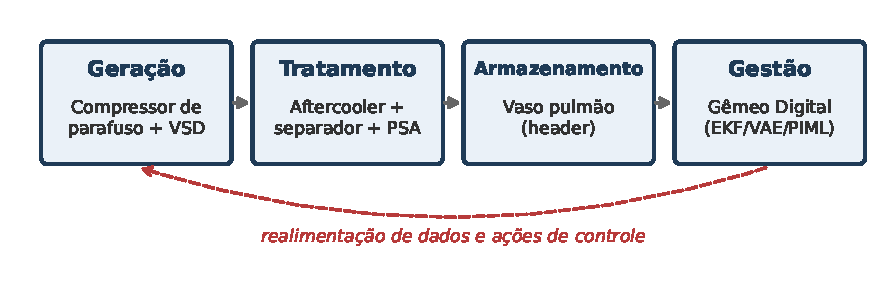
\includegraphics[width=0.75\textwidth]{figuras/fig_2_2_arquitetura.pdf}
		\caption[Diagrama de blocos da arquitetura do sistema]{Diagrama de blocos da arquitetura do sistema: os quatro pilares funcionais e a realimentação do Gêmeo Digital sobre a planta física.}
		\label{fig:2-1}
	\end{figure}

	\subsection{\textbf{Princípio de Funcionamento do Compressor de Parafuso}}
	Antes de qualquer equacionamento, é necessário compreender o princípio físico que gera a compressão: dois rotores helicoidais — o macho, com lóbulos convexos, e a fêmea, com cavidades côncavas — giram engrenados dentro de uma carcaça cilíndrica dupla \cite{hanlon}. A relação de lóbulos mais comum é $4{:}6$ (quatro lóbulos no macho para seis cavidades na fêmea), um perfil assimétrico desenvolvido para minimizar as áreas de vedação e o vazamento interno \cite{lysholm}. A Figura~\ref{fig:2-2} mostra o perfil real desse engrenamento assimétrico (aqui numa relação $5{:}6$, mesmo princípio geométrico) — repare como o contorno de um rotor é o negativo do outro, mantendo contato de vedação contínuo ao longo de toda a rotação.

	\begin{figure}[h!tbp]
		\centering
		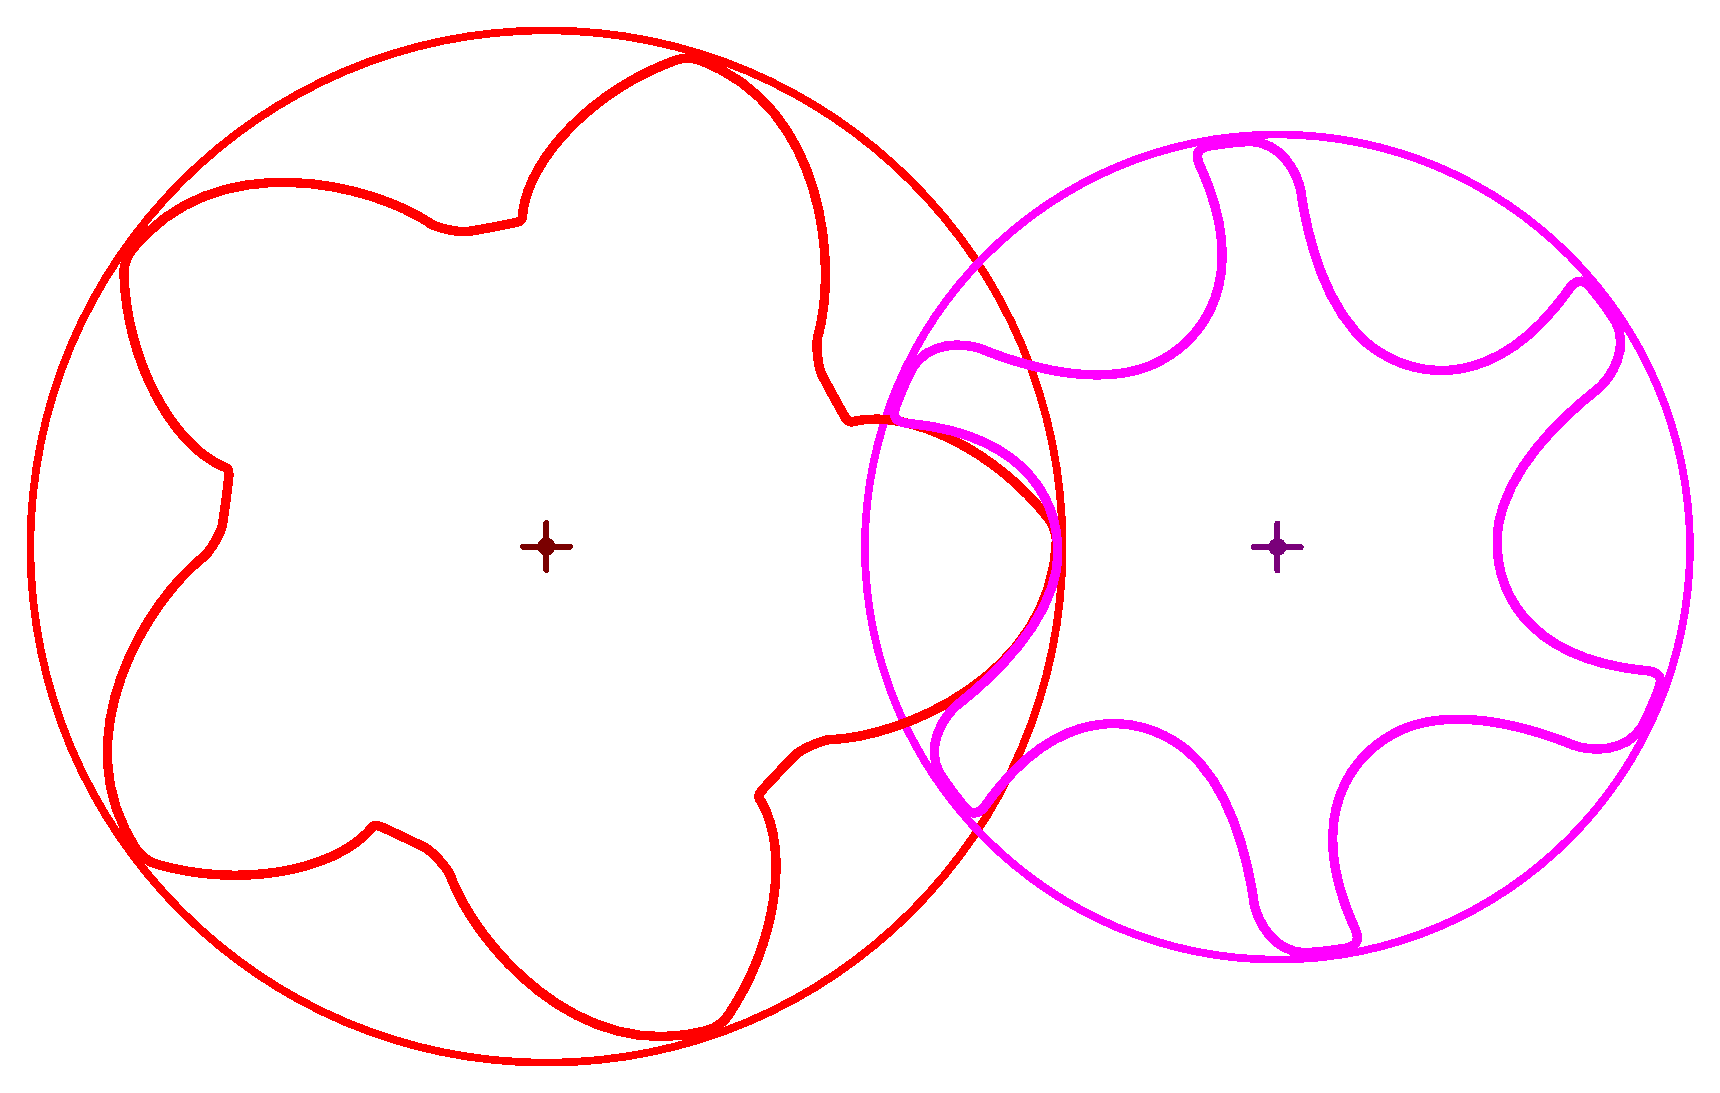
\includegraphics[width=0.60\textwidth]{figuras/fig_2_1_rotores.pdf}
		\caption[Perfil de engrenamento assimétrico de rotores helicoidais]{Perfil de engrenamento assimétrico de rotores helicoidais (relação 5:6), com centros dos eixos indicados. Adaptado de \textit{Asymmetric Screw Compressor Rotor Mesh}, Slashme, Wikimedia Commons, licença CC BY-SA 4.0 (traços reforçados e marcadores de centro adicionados pelo autor).}
		\label{fig:2-2}
	\end{figure}

	O ciclo de trabalho ocorre em três fases sequenciais, repetidas continuamente a cada engrenamento:
	\begin{enumerate}
		\item \textbf{Admissão:} À medida que os rotores giram e se desengrenam na extremidade de sucção, uma câmara em forma de ``V'' se abre entre os lóbulos e a carcaça, e o ar atmosférico preenche esse volume crescente.
		\item \textbf{Compressão:} Conforme a rotação avança, o ponto de engrenamento entre macho e fêmea se desloca ao longo do comprimento helicoidal dos rotores, fechando progressivamente a câmara e reduzindo seu volume — é essa redução puramente geométrica, sem válvulas de admissão ou descarga no sentido alternativo, que caracteriza a compressão como um processo de deslocamento positivo contínuo (ao contrário do compressor alternativo, que comprime em pulsos, ou do centrífugo, que comprime por troca de quantidade de movimento).
		\item \textbf{Descarga:} Quando a câmara em compressão alcança a aresta da porta de descarga — posição fixada pela geometria da carcaça, não por uma válvula —, o volume comprimido é liberado para a linha de descarga. É exatamente essa posição fixa da aresta de descarga que define a razão volumétrica interna $V_i$, detalhada mais adiante neste documento.
	\end{enumerate}
	Nos compressores do escopo deste documento (isentos de óleo), não há filme de óleo na câmara de trabalho para transmitir torque de um rotor ao outro por contato direto; por isso os dois eixos são sincronizados externamente por um par de engrenagens de precisão (\textit{timing gears}), mantendo uma folga constante e sem contato metal-metal entre os lóbulos durante toda a rotação — mecanismo cuja dinâmica é modelada em capítulo posterior.

	\subsection{\textbf{Cadeia de Geração e Compressão}}
	A unidade central é o compressor de parafuso rotativo, classificado como uma máquina de deslocamento positivo.
	\begin{itemize}
		\item \textbf{Rotores Helicoidais:} O par de rotores (macho e fêmea) reduz o volume do ar admitido através do engrenamento contínuo.
		\item \textbf{Motor Elétrico e VSD:} O acionamento é realizado por um motor de indução trifásico. O inversor de frequência (\textit{Variable Speed Drive} - VSD) modula a velocidade angular $\omega$ para parear a vazão produzida com a demanda da planta, operando na faixa de pressão de $7\,\text{bar}$ a $10\,\text{bar}$.
	\end{itemize}

	Para visualizar como esses elementos se conectam fisicamente — do acionamento elétrico até a descarga final de alta pressão —, a Figura~\ref{fig:2-3} apresenta o trem de compressão completo em perspectiva 3D: o motor elétrico aciona a caixa multiplicadora (gearbox) através de um acoplamento flexível; a gearbox distribui a rotação para os dois estágios de compressão (pinhões LP e HP engrenados à coroa central, mesma cinemática detalhada no Capítulo de Engenharia do Trem de Transmissão); o ar atmosférico admitido no estágio de baixa pressão (LP) é resfriado no intercooler antes de seguir para o estágio de alta pressão (HP), de onde é descarregado para o tratamento posterior (aftercooler e secagem, detalhados nos capítulos seguintes). É um esquema ilustrativo, não um desenho de projeto: motor, gearbox e tubulação são representados por formas geométricas simples, enquanto os dois pares de rotores reaproveitam a mesma técnica de varredura helicoidal usada no render do elemento compressor isolado apresentado no capítulo seguinte, em escalas proporcionalmente diferentes entre os estágios LP e HP (o de menor pressão é fisicamente maior, o de maior pressão é mais compacto).

	\begin{figure}[h!tbp]
		\centering
		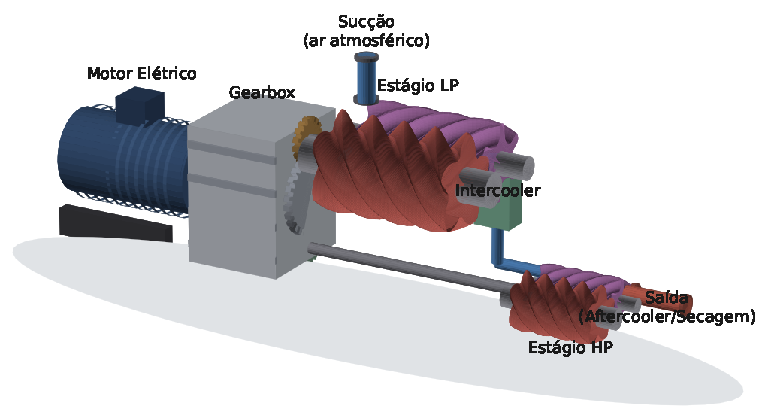
\includegraphics[width=0.80\textwidth]{figuras/fig_2_3_conjunto3d.pdf}
		\caption[Trem de compressão completo em perspectiva 3D]{Trem de compressão completo em perspectiva 3D — do motor elétrico ao estágio HP e à saída para tratamento, passando pela gearbox e pelo intercooler. Esquema ilustrativo; motor, gearbox e tubulação são formas 3D simplificadas, e os pares de rotores reaproveitam a varredura helicoidal do perfil de engrenamento adaptado de \textit{Asymmetric Screw Compressor Rotor Mesh}, Slashme, Wikimedia Commons, licença CC BY-SA 4.0.}
		\label{fig:2-3}
	\end{figure}

	\subsection{\textbf{Subsistema de Resfriamento e Separação}}
	Devido ao processo de compressão ser aproximadamente adiabático, a temperatura do ar na descarga do elemento compressor é elevada.
	\begin{itemize}
		\item \textbf{Aftercooler (Resfriador Posterior):} Trocador de calor que utiliza água do mar ou ar ambiente para reduzir a temperatura do ar comprimido.
		\item \textbf{Separador de Condensado:} Dispositivo que remove a água líquida precipitada após o resfriamento.
	\end{itemize}

	\subsection{\textbf{Invólucro do Pacote (Hood) e Ventilação Forçada}}
	Além do calor rejeitado pelo próprio ar comprimido nos trocadores de processo, o pacote compressor dissipa uma quantidade significativa de calor \textbf{para dentro do seu próprio invólucro} (\textit{hood}/\textit{canopy} acústico): perdas do motor elétrico, do VSD, da caixa multiplicadora e a própria superfície quente do elemento compressor e da tubulação interna aquecem o ar confinado dentro do gabinete. Um exaustor força a saída desse ar quente e a entrada de ar ambiente renovado, evitando que a temperatura interna do invólucro comprometa a eletrônica de potência e o isolamento do motor.
	\begin{itemize}
		\item \textbf{Fontes de Calor Internas ao Invólucro ($\dot{Q}_{\text{gerado}}$):} A soma das perdas térmicas de todos os componentes que dissipam calor para dentro do gabinete, já modeladas individualmente nos capítulos anteriores — perdas do motor, do VSD (Equação~\eqref{eq:s4-3}), da gearbox (Equação~\eqref{eq:s5-2}) e a convecção/radiação da carcaça quente do elemento compressor ($\dot{Q}_{\text{casco}}$), conforme a Equação~\eqref{eq:s2-1}:
		\begin{equation}\label{eq:s2-1}
\dot{Q}_{\text{gerado}} = \dot{W}_{\text{mot}}(1 - \eta_{\text{mot}}) + P_{\text{loss,VSD}} + P_{\text{loss,gb}} + \dot{Q}_{\text{casco}}
\end{equation}
		\item \textbf{Capacidade de Remoção do Exaustor ($\dot{Q}_{\text{hood}}$):} A Equação~\eqref{eq:s2-2} calcula quanto calor o exaustor efetivamente remove, em função da vazão mássica de ar de ventilação forçada pelo exaustor ($\dot{m}_{\text{vent}}$) e do aumento de temperatura entre a admissão de ar renovado e a exaustão do ar quente:
		\begin{equation}\label{eq:s2-2}
\dot{Q}_{\text{hood}} = \dot{m}_{\text{vent}} \cdot c_p \cdot (T_{\text{exaustão}} - T_{\text{amb}})
\end{equation}
		Em regime permanente, o invólucro só mantém temperatura interna estável se $\dot{Q}_{\text{hood}} \ge \dot{Q}_{\text{gerado}}$; a folga entre os dois lados dessa desigualdade é a margem de projeto da ventilação forçada.
		\item \textbf{Mecanismo de Falha:} Obstrução do filtro de admissão do exaustor, pá do ventilador danificada, motor do exaustor em falha, ou obstrução das venezianas de exaustão por sujeira/sal — qualquer um reduz $\dot{m}_{\text{vent}}$ e desequilibra a Equação~\eqref{eq:s2-2}.
		\item \textbf{Detecção:} Aumento progressivo de $T_{\text{exaustão}}$ para a mesma carga térmica interna estimada é o indicador primário; o Gêmeo Digital deve correlacionar esse aumento com o fator de desclassificação (\textit{derating}) do VSD (Capítulo de Subsistema Elétrico) e com a degradação acelerada do isolamento do motor pela Equação de Arrhenius (Equação~\eqref{eq:s4-7}) — ambos amplificados por uma falha silenciosa de ventilação do invólucro.
		\item \textbf{Função Acústica do Invólucro:} O mesmo gabinete modelado termicamente acima cumpre, simultaneamente, o papel de barreira de ruído — daí o qualificativo \textit{canopy acústico} usado desde a abertura desta seção. O nível de pressão sonora garantido do pacote é medido e declarado segundo a ISO 2151 \cite{iso2151}, código de ensaio específico para compressores e bombas de vácuo (a própria ISO 1217, já citada no Capítulo 1 para o FAD, exclui explicitamente ensaios de ruído do seu escopo e remete a essa norma). O limite típico de exposição ocupacional a bordo é o que dimensiona a atenuação exigida do invólucro — um requisito independente da ventilação forçada, e por vezes conflitante com ela: mais área de abertura para vazão de ar de resfriamento tende a reduzir a atenuação acústica, de modo que o projeto do exaustor não pode ser otimizado isoladamente do requisito de ruído.
	\end{itemize}

	\subsection{\textbf{Tratamento de Ar (Secagem e Filtragem)}}
	Para atender aos padrões de ar de instrumentação, o fluido deve passar por um processo de purificação rigoroso.
	\begin{itemize}
		\item \textbf{Secadora PSA (\textit{Pressure Swing Adsorption}):} Composta por duas torres preenchidas com material dessecante. Enquanto uma torre adsorve a umidade sob alta pressão, a outra regenera-se através da expansão de uma parte do ar seco (purga).
		\item \textbf{Trens de Filtragem:} Filtros coalescentes e de partículas que removem aerossóis de óleo e contaminantes sólidos.
	\end{itemize}
	
	\subsection{\textbf{Vaso de Pressão (Pulmão de Armazenamento)}}
	O reservatório de ar comprimido atua como um amortecedor de pulsações e um buffer de energia.
	\begin{itemize}
		\item \textbf{Função Estabilizadora:} Compensa picos de demanda sem causar quedas bruscas na pressão de linha.
		\item \textbf{Cálculo de Capacidade:} O volume do vaso $V_{\text{res}}$ é dimensionado com base na variação de pressão permitida $\Delta P$, pela Equação~\eqref{eq:s2-3}:
		\begin{equation}\label{eq:s2-3}
 V_{\text{res}} = \frac{t \cdot (\dot{V}_{\text{consumo}} - \dot{V}_{\text{comp}}) \cdot P_{\text{atm}}}{\Delta P} 
\end{equation}
		Onde $t$ é o tempo de autonomia desejado (intervalo em que o vaso deve sustentar sozinho o déficit entre consumo e produção antes que $\Delta P$ seja excedido).
	\end{itemize}
	
	\subsection{\textbf{Gestor de Pressão e Monitoramento de Consumo}}
	A gestão do sistema é realizada por um controlador lógico que atua como a interface primária para o Gêmeo Digital.
	\begin{itemize}
		\item \textbf{Transdutores de Pressão:} Instalados em pontos estratégicos para monitorar perdas de carga ($\Delta P_{\text{filtros}}$).
		\item \textbf{Medidores de Vazão:} Sensores que quantificam o consumo real da plataforma.
		\item \textbf{Lógica de Controle:} Mantém a pressão de rede em um \textit{setpoint} ajustando a rampa do VSD.
	\end{itemize}

	\subsection{\textbf{Fechamento Térmico do Invólucro}}
	As Equações~\eqref{eq:s2-1} e~\eqref{eq:s2-2} definem, respectivamente, a carga térmica gerada dentro do invólucro e a capacidade do exaustor de removê-la, mas nenhuma das duas fecha qual temperatura de regime permanente o ar confinado atinge — a mesma lacuna que o Capítulo 9 tinha para a carcaça do estágio LP antes de ser fechada. O caminho de ventilação forçada tem uma \textbf{entrada}, de ar externo renovado admitido pelo exaustor à temperatura ambiente $T_{amb}$, e uma \textbf{saída}, do mesmo ar já aquecido pela carga térmica interna e descarregado à temperatura $T_{\text{exaustão}}$ — as duas pontas já presentes na própria Equação~\eqref{eq:s2-2}. Assumindo mistura completa do ar confinado (o ar de exaustão representa a própria temperatura interna do invólucro, $T_{\text{hood}} \equiv T_{\text{exaustão}}$) e substituindo a Equação~\eqref{eq:s2-1} na~\eqref{eq:s2-2} em regime permanente ($\dot Q_{\text{hood}} = \dot Q_{\text{gerado}}$, a condição de estabilidade já discutida ali), chega-se à Equação~\eqref{eq:s2-4}:
	\begin{equation}\label{eq:s2-4}
 T_{\text{hood}} = T_{amb} + \frac{\dot{Q}_{\text{gerado}}}{\dot{m}_{\text{vent}} \cdot c_p}
\end{equation}
	Essa é a temperatura que efetivamente banha todo equipamento confinado no mesmo invólucro — motor, VSD, gearbox e a carcaça do elemento compressor —, não $T_{amb}$ externo. Isso importa diretamente para o fechamento do balanço térmico da carcaça feito no Capítulo 9 (Equações~\eqref{eq:s9-14}--\eqref{eq:s9-17}): aquelas equações usam $T_{amb}$ como referência de convecção, o que é correto apenas para uma instalação a céu aberto, sem invólucro. No arranjo mais comum em plantas offshore por restrição de ruído — motor, gearbox e os dois estágios de compressão dentro do mesmo \textit{canopy} acústico, como descrito na abertura desta seção —, a referência correta nas Equações~\eqref{eq:s9-15}--\eqref{eq:s9-17} é $T_{\text{hood}}$ da Equação~\eqref{eq:s2-4}, não a temperatura ambiente externa.

	Isso também resolve uma aparente circularidade entre os dois capítulos: o termo $\dot{Q}_{\text{casco}}$ da Equação~\eqref{eq:s2-1} é a mesma grandeza física que o Capítulo 9 soma como $\dot{Q}_{\text{ext}} + \dot{Q}_{\text{arref}}$ — o calor que a carcaça entrega ao ar do invólucro por convecção (natural mais forçada). Em regime permanente esse total iguala $\dot{Q}_{\text{int}}$ (Equação~\eqref{eq:s9-14}, pela própria Equação~\eqref{eq:s9-6}), de modo que $\dot{Q}_{\text{casco}} = \dot{Q}_{\text{int}}$ pode ser calculado diretamente a partir da perda mecânica do estágio LP, sem exigir $T_c$ como entrada. A ordem de cálculo correta é, portanto, sequencial e não simultânea: (1) $\dot{Q}_{\text{int}}$ pela Equação~\eqref{eq:s9-14}, a partir do ponto de operação; (2) $\dot{Q}_{\text{gerado}}$ (Equação~\eqref{eq:s2-1}, usando $\dot{Q}_{\text{casco}}=\dot{Q}_{\text{int}}$) e $T_{\text{hood}}$ (Equação~\eqref{eq:s2-4}); (3) $T_c$ (Equação~\eqref{eq:s9-16}, agora referenciada a $T_{\text{hood}}$). Para instalações sem invólucro — compressor a céu aberto —, esta subseção inteira não se aplica: a carcaça convecciona diretamente para $T_{amb}$, como nas Equações~\eqref{eq:s9-15}--\eqref{eq:s9-17} originais.

	\vspace{1em}
	\hrule
	\vspace{1em}

	\textbf{Diretriz Técnica Final:} A arquitetura descrita aqui — geração por parafuso isento de óleo, tratamento por resfriamento/secagem e armazenamento em vaso pulmão — define os quatro blocos físicos que o Gêmeo Digital deve modelar de forma acoplada; tratar qualquer um isoladamente (por exemplo, otimizar o compressor sem considerar o impacto na secadora a jusante) produz um modelo incompleto e recomendações potencialmente contraditórias. A Equação~\eqref{eq:s2-4} acrescenta uma consequência prática direta para instalações com invólucro acústico: qualquer equação térmica de um componente interno (Equação~\eqref{eq:s9-6} da carcaça, entre outras) só está correta se referenciada a $T_{\text{hood}}$, não à ambiente externa — usar $T_{amb}$ nesse contexto subestima sistematicamente a temperatura real de operação.

	% --- Fim do Capítulo 2 ---
	
	% --- Início do Capítulo 3 ---
	
	\clearpage
	\section{\textbf{Detalhamento de Componentes, Acessórios e Instrumentação}}
	
	Antes de detalhar cada subsistema individualmente, é útil visualizar o coração do pacote: o elemento compressor (airend), onde os dois rotores helicoidais executam fisicamente a compressão. A Figura~\ref{fig:3-1} apresenta o par de rotores em perspectiva tridimensional, obtida por varredura helicoidal do mesmo perfil de engrenamento assimétrico $5{:}6$ já apresentado na Figura~\ref{fig:2-2}: o rotor macho (à direita) recebe uma torção total de $300^\circ$ ao longo do comprimento, enquanto a fêmea gira em sentido contrário com hélice oposta, na razão $5/6$ da torção do macho — exatamente a relação cinemática que mantém o contato de vedação contínuo durante a rotação. Os tocos de eixo nas extremidades são os assentos dos rolamentos e, no lado de acionamento, a interface com a caixa multiplicadora (gearbox). As subseções seguintes detalham os blocos que cercam esse núcleo — motor elétrico, acoplamento, gearbox e acessórios — e sua instrumentação associada, seguindo a mesma organização por subsistema já consolidada na literatura de referência sobre tecnologia de compressores \cite{bloch}.

	\begin{figure}[h!tbp]
		\centering
		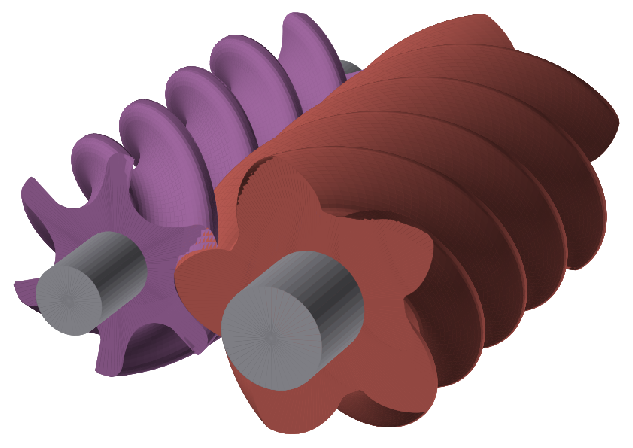
\includegraphics[width=0.80\textwidth]{figuras/fig_3_1_parafuso3d.pdf}
		\caption[Par de rotores helicoidais do elemento compressor (3D)]{Par de rotores helicoidais do elemento compressor (airend) em perspectiva 3D, gerado por varredura helicoidal do perfil de engrenamento da Figura~\ref{fig:2-2} (torção de $300^\circ$ no rotor macho, relação $5{:}6$, hélices opostas). Elaboração 3D original do autor; perfil 2D adaptado de \textit{Asymmetric Screw Compressor Rotor Mesh}, Slashme, Wikimedia Commons, licença CC BY-SA 4.0.}
		\label{fig:3-1}
	\end{figure}

	\subsection{\textbf{Subsistema de Potência e Acionamento}}
	\begin{itemize}
		\item \textbf{Painel Elétrico e VSD:} O painel elétrico é o ponto de entrega de energia do pacote — recebe a alimentação de média/baixa tensão da plataforma, protege o circuito com relés de disparo (detalhados no Capítulo de Subsistema Elétrico) e abriga o Inversor de Frequência (\textit{Variable Speed Drive}, VSD). O VSD converte a frequência fixa da rede numa frequência variável, permitindo modular a velocidade angular $\omega$ do motor para casar a vazão produzida com a demanda da planta em vez de operar sempre a rotação nominal. O efeito colateral desse chaveamento eletrônico de alta frequência é a distorção harmônica total de corrente ($\text{THD}_i$) injetada na rede — quanto maior a distorção, maior o aquecimento adicional no motor e a interferência em outros equipamentos sensíveis da rede elétrica isolada da plataforma, por isso ela é monitorada e mitigada (filtros de linha, técnicas de modulação PWM).
		\item \textbf{Motor Elétrico:} Motor de indução trifásico responsável por converter a energia elétrica recebida do VSD em energia mecânica no eixo, entregue ao trem de potência (Capítulo de Trem de Potência). A eficiência de conversão $\eta_{\text{mot}}$ é a razão entre a potência mecânica efetivamente disponível no eixo e a potência elétrica consumida — a diferença entre as duas é dissipada como calor nos enrolamentos e no núcleo, e é justamente essa parcela de perda que aquece o motor e limita sua vida útil. O circuito equivalente completo, o escorregamento e os mecanismos de falha elétrica (incluindo desbalanço entre fases) são modelados em detalhe no Capítulo de Subsistema Elétrico.
	\end{itemize}
	
	\subsection{\textbf{Unidade Compressora e Circuito de Óleo}}
	\begin{itemize}
		\item \textbf{Elemento Compressor:} É o próprio par de rotores helicoidais (\textit{airend}) apresentado na Figura~\ref{fig:3-1} — o núcleo físico onde a compressão de fato acontece, por redução geométrica contínua do volume entre os lóbulos em engrenamento (ciclo já descrito no Capítulo de Arquitetura). A vazão mássica teórica que ele entrega, Equação~\eqref{eq:s3-1}, é o produto da densidade do ar de sucção pelo volume deslocado pelo par de rotores a cada rotação completa ($V_{\text{disp}}$, fixado pela geometria do perfil helicoidal — comprimento, diâmetro e ângulo de hélice dos rotores) e pela rotação, corrigido pela eficiência volumétrica real $\eta_{\text{vol}}$:
		\begin{equation}\label{eq:s3-1}
 \dot{m} = \rho \cdot V_{\text{disp}} \cdot \frac{\omega}{2\pi} \cdot \eta_{\text{vol}}
\end{equation}
		O termo $\eta_{\text{vol}}$ é o que separa a vazão teórica (puramente geométrica) da vazão real: parte do ar comprimido escapa de volta para câmaras de pressão mais baixa através das folgas microscópicas entre rotores e carcaça, um mecanismo detalhado no Capítulo de Termodinâmica do Estágio LP. Quanto maior o desgaste dessas folgas ao longo da vida do equipamento, menor $\eta_{\text{vol}}$ e maior o desvio entre a vazão prevista por esta equação e a vazão real entregue à rede.
		\item \textbf{Separador de Ar/Óleo (Deaeração do Circuito de Lubrificação):} Como o compressor deste documento é isento de óleo na câmara de compressão (não há óleo em contato com o ar de processo), este separador não atua no ar comprimido em si, mas no óleo de lubrificação da gearbox e dos mancais: o óleo que retorna ao cárter após lubrificar engrenagens e mancais chega aerado (com bolhas de ar incorporadas pelo respingo/turbulência do engrenamento), e precisa liberar esse ar antes de ser recirculado pela bomba — óleo aerado perde capacidade de sustentar o filme lubrificante e de dissipar calor. A perda de carga que esse separador impõe ao próprio óleo, $\Delta P_{\text{sep}}$, é monitorada porque seu aumento progressivo indica saturação ou obstrução do elemento.
	\end{itemize}
	
	\subsection{\textbf{Resfriamento e Drenagem}}
	\begin{itemize}
		\item \textbf{Aftercooler:} É o trocador de calor final do pacote, posicionado logo após a descarga do último estágio de compressão (HP) e antes da filtragem/secagem. Sua função é reduzir a temperatura do ar — tipicamente acima de $100\,^{\circ}\text{C}$ na saída do estágio HP — para um patamar compatível com os elementos filtrantes e, principalmente, para forçar a condensação da umidade que o ar carrega antes que ela chegue ao secador PSA (detalhado no Capítulo de Secagem). Normalmente é resfriado a água do mar ou a ar ambiente, conforme a disponibilidade na plataforma. Sua taxa de rejeição térmica, Equação~\eqref{eq:s3-2}, segue a forma clássica de projeto de trocadores — coeficiente global de transferência ($U$, que piora com incrustação/\textit{fouling}) vezes área de troca ($A$, fixa por projeto) vezes a diferença de temperatura média logarítmica ($\Delta T_{\text{LMTD}}$, detalhada no Capítulo de Dinâmica do Intercooler):
		\begin{equation}\label{eq:s3-2}
 \dot{Q} = U \cdot A \cdot \Delta T_{\text{LMTD}}
\end{equation}
		Como $A$ é fixa, qualquer queda na taxa de calor removido para a mesma vazão e mesma diferença de temperatura de entrada só pode ser explicada por uma queda em $U$ — é esse raciocínio que permite ao Gêmeo Digital atribuir uma perda de performance térmica à incrustação do trocador, e não a outra causa.
		\item \textbf{Drenos Automáticos:} Válvulas que removem periodicamente a água líquida que se acumula no fundo do vaso separador de condensado, logo após o aftercooler — o mesmo condensado quantificado no Capítulo de Intercooler. Podem ser acionadas por um sensor de nível (abrem só quando há líquido acumulado, mais eficiente) ou por temporizador (abrem em ciclos fixos, mais simples porém desperdiça ar comprimido a cada purga). Um dreno que trava aberto perde ar de processo continuamente; um que trava fechado permite que a água se acumule e seja arrastada para os estágios seguintes — ambos os modos de falha são detalhados no Capítulo de Aftercooler e Filtragem.
	\end{itemize}
	
	\subsection{\textbf{Purificação e Secagem (Sistema PSA)}}
	\begin{itemize}
		\item \textbf{Torres de Adsorção:} Duas colunas cilíndricas preenchidas com material dessecante (tipicamente \textbf{Alumina Ativada} ou peneira molecular) que retém fisicamente as moléculas de vapor d'água na superfície de seus grãos porosos à medida que o ar úmido passa por elas sob pressão. O princípio de adsorção por oscilação de pressão (\textit{Pressure Swing Adsorption}, PSA) alterna as duas torres entre dois papéis: enquanto uma seca o ar de processo, a outra é regenerada — o ciclo completo, a cinética de saturação do leito e o cálculo do ponto de orvalho resultante são detalhados no Capítulo de Sistema de Secagem.
		\item \textbf{Resistências de Aquecimento:} Utilizadas nos ciclos de regeneração térmica dos secadores que precisam de calor externo para ``expulsar'' a umidade retida no dessecante saturado (ao contrário dos secadores PSA a frio, que regeneram apenas por expansão do ar de purga). A Equação~\eqref{eq:s3-3} calcula a potência elétrica necessária como a vazão mássica de ar de purga vezes o calor específico do ar vezes o salto de temperatura imposto a esse ar de regeneração:
		\begin{equation}\label{eq:s3-3}
 P_{\text{term}} = \dot{m}_{\text{purge}} \cdot c_p \cdot \Delta T
\end{equation}
		Esse consumo elétrico de regeneração é significativo o suficiente para justificar a recuperação de calor residual de outras partes do pacote (aftercooler, óleo, exaustão do invólucro), estratégia detalhada no Capítulo de Sistema de Secagem.
		\item \textbf{Válvulas de Comutação:} Válvulas solenoides que alternam o caminho do fluxo de ar entre as duas torres a cada ciclo — direcionando o ar úmido de processo para a torre em adsorção e o ar de purga (ou o ar quente de regeneração) para a torre que está sendo regenerada. Uma falha de comutação (válvula presa ou com vazamento entre torres) compromete a secagem mesmo com o leito dessecante em boas condições, por isso é diagnosticada separadamente da saturação do próprio material.
	\end{itemize}
	
	\subsection{\textbf{Filtragem e Válvulas de Linha}}
	\begin{itemize}
		\item \textbf{Filtros Coalescentes:} Elementos filtrantes de meio fibroso instalados a jusante do aftercooler que capturam aerossóis finos de óleo (do circuito de lubrificação) e partículas sólidas residuais, protegendo o leito dessecante do secador PSA — o material adsorvente é facilmente contaminado e perde capacidade permanentemente se exposto a óleo. À medida que o meio filtrante retém contaminantes, a perda de carga que ele impõe ao escoamento cresce; a Equação~\eqref{eq:s3-4} modela essa perda pela forma clássica de perda de carga localizada — coeficiente de perda do elemento filtrante ($\zeta$, que cresce com a saturação) vezes a pressão dinâmica do escoamento:
		\begin{equation}\label{eq:s3-4}
 \Delta P = \zeta \cdot \frac{\rho v^2}{2}
\end{equation}
		Como $\rho$ e $v$ variam com a condição de operação, o Gêmeo Digital normaliza $\Delta P$ medido por essas duas variáveis antes de comparar contra o limite de substituição do elemento — comparar $\Delta P$ bruto entre duas condições de carga distintas levaria a falsos alarmes.
		\item \textbf{Válvulas de Bloqueio e Retenção:} Duas famílias com papéis distintos: as válvulas de \textbf{bloqueio} (manuais ou motorizadas) isolam trechos da tubulação para manutenção sem despressurizar todo o sistema; as válvulas de \textbf{retenção} (\textit{check valves}) permitem o fluxo em um único sentido e impedem que o ar armazenado no vaso pulmão reflua para o compressor quando este for parado ou perder pressão — sem elas, a parada de uma unidade em operação em frota (Capítulo de Distribuição e Armazenamento) despressurizaria seu próprio circuito através da rede comum.
	\end{itemize}
	
	\subsection{\textbf{Armazenamento e Segurança}}
	\begin{itemize}
		\item \textbf{Vaso de Pressão (Pulmão):} Reservatório cilíndrico de ar já seco e filtrado, dimensionado conforme ASME Seção VIII Div. 1 para operar até aproximadamente $10\,\text{bar}$. Funciona como um amortecedor de pulsações e um buffer de energia entre a produção (descontínua, sujeita a ciclos de carga/alívio do compressor) e o consumo da planta — sem ele, cada oscilação de demanda se propagaria diretamente para a pressão de rede. Sua dinâmica de pressão interna, Equação~\eqref{eq:s3-5}, é proporcional ao desbalanço instantâneo entre a vazão que entra (produção) e a que sai (consumo da planta):
		\begin{equation}\label{eq:s3-5}
 \frac{dP_{\text{res}}}{dt} = \frac{R T}{V} \Delta \dot{m}
\end{equation}
		Quando $\Delta \dot{m} = 0$ (produção e consumo equilibrados), a pressão do vaso permanece constante; um $\Delta \dot{m}$ persistentemente negativo (consumo maior que produção) é o sinal precoce de que a rede está prestes a atingir um nível de alarme de pressão baixa (Capítulo de Distribuição e Armazenamento).
		\item \textbf{PSV (Válvula de Segurança):} \textit{Pressure Safety Valve} — dispositivo puramente mecânico, independente de qualquer lógica de controle ou instrumentação eletrônica, que abre automaticamente por ação de mola quando a pressão interna excede um limite pré-ajustado, aliviando o excesso para a atmosfera. É a última camada de proteção contra sobrepressão do vaso, exigida pela norma ASME VIII como redundância física ao controle de pressão normal do sistema — mesmo que toda a lógica de controle do Gêmeo Digital falhe, a PSV continua protegendo o equipamento. \textbf{Nota de escopo:} o dimensionamento do orifício de alívio (área mínima de passagem exigida pela ASME VIII Div. 1 \cite{asme8} para a condição de sobrepressão de projeto) é matéria de projeto do vaso, resolvida uma única vez na especificação do equipamento — não uma grandeza que o Gêmeo Digital calcula ou monitora em operação. O papel do modelo aqui se limita a detectar os dois modos de falha operacional da PSV já instrumentada (travada aberta ou fechada), não a substituir o cálculo de dimensionamento.
	\end{itemize}
	
	\subsection{\textbf{Instrumentação}}
	\begin{itemize}
		\item \textbf{Transdutores e Sensores:} O conjunto de pontos de medição distribuídos ao longo de todo o trem descrito neste capítulo — pressão ($P$) em cada estágio e no vaso pulmão, temperatura ($T$) na descarga de cada trocador, umidade relativa ($\phi$) e ponto de orvalho sob pressão ($T_{dp}$) na saída do secador. Nenhuma das equações apresentadas neste capítulo é calculável pelo Gêmeo Digital sem que a variável correspondente esteja de fato instrumentada em campo — é por isso que a Diretriz Técnica Final abaixo trata a cobertura de instrumentação como um limite físico do modelo, não um detalhe de implementação.
	\end{itemize}

	\vspace{1em}
	\hrule
	\vspace{1em}

	\textbf{Diretriz Técnica Final:} Cada componente listado neste capítulo é, ao mesmo tempo, um ponto físico de instrumentação e uma entrada do modelo matemático desenvolvido nos capítulos seguintes — a qualidade do Gêmeo Digital é limitada pela cobertura e pela taxa de amostragem desses sensores, não apenas pela sofisticação do equacionamento.

	% --- Fim do Capítulo 3 ---
	
	% --- Início do Capítulo 4: Subsistema Elétrico e Acionamento Dinâmico ---
	
	\clearpage
	\section{\textbf{Subsistema Elétrico e Acionamento Dinâmico}}
	
	Este capítulo detalha a modelagem do fluxo de energia desde o painel de distribuição até o eixo do compressor, integrando eletrônica de potência, eletromagnetismo e a modelagem matemática de modos de falha para o Gêmeo Digital.
	
	\subsection{\textbf{Painel Elétrico e Lógica de Proteção (Relés)}}
	O painel elétrico offshore atua como a interface de segurança primária. Os relés de proteção digitais monitoram a integridade do sistema através de curvas de tempo inverso, que devem ser replicadas no Gêmeo Digital para prever disparos (\textit{trips}) indesejados.
	
	\begin{itemize}
		\item \textbf{Equacionamento de Disparo (Norma IEC 60255 \cite{iec60255}):}
		O tempo de atuação $t_{\text{trip}}$ é modelado pela Equação~\eqref{eq:s4-1} para detectar sobrecargas térmicas antes que ocorram danos permanentes:
		\begin{equation}\label{eq:s4-1}
 t_{\text{trip}} = \frac{k_{\text{relé}} \cdot \beta}{\left( \frac{I}{I_s} \right)^\alpha - 1} 
\end{equation}
		Onde:
		\begin{itemize}
			\item $I$: Corrente de carga medida em tempo real.
			\item $I_s$: Corrente de ajuste (setpoint).
			\item $\alpha, \beta, k_{\text{relé}}$: Constantes que definem a curva (Normalmente Inversa, Muito Inversa ou Extremamente Inversa); $k_{\text{relé}}$ é subscrito para não colidir com o índice de tempo discreto $k$ usado nos capítulos de EKF/MPC/PSO.
		\end{itemize}
		\item \textbf{Mecanismos de Falha no Painel:} O Gêmeo Digital monitora a resistência de contato e a temperatura nos barramentos. Um aumento na temperatura $T_{\text{contato}}$ sem aumento de corrente indica oxidação ou afrouxamento mecânico por vibração.
	\end{itemize}
	
	\subsection{\textbf{Inversor de Frequência (VSD - Variable Speed Drive)}}
	O VSD é o elemento de controle que modula a velocidade angular $\omega$ do motor. Ele é modelado como um conversor de potência com perdas não lineares.
	
	\begin{itemize}
		\item \textbf{Controle V/f (Tensão/Frequência):} Para manter o fluxo magnético constante no motor e evitar a saturação do núcleo, o VSD eleva a tensão de saída ($V_{\text{out}}$) na mesma proporção em que eleva a frequência ($f_{\text{out}}$), mantendo a razão entre as duas praticamente fixa em toda a faixa de rotação — relação conhecida como Equação~\eqref{eq:s4-2}:
		\begin{equation}\label{eq:s4-2}
 \frac{V_{\text{out}}}{f_{\text{out}}} \approx \text{constante}
\end{equation}
		\item \textbf{Eficiência e Perdas Térmicas:} A potência dissipada no VSD ($P_{\text{loss,VSD}}$) é fundamental para o prognóstico de falha dos módulos IGBT. A Equação~\eqref{eq:s4-3} decompõe essa dissipação em duas parcelas de origem física distinta: $P_{\text{switching}}$, a perda toda vez que o IGBT liga/desliga (proporcional à frequência de chaveamento), e $P_{\text{conduction}}$, a perda resistiva enquanto o IGBT permanece conduzindo corrente:
		\begin{equation}\label{eq:s4-3}
 P_{\text{loss,VSD}} = P_{\text{switching}} + P_{\text{conduction}}
\end{equation}
		A eficiência instantânea é dada por $\eta_{\text{vsd}} = \frac{P_{\text{out}}}{P_{\text{in}}}$. O Gêmeo Digital utiliza a distorção harmônica total ($\text{THD}_i$) para calcular o fator de desclassificação (\textit{derating}) do motor.
	\end{itemize}
	
	\subsection{\textbf{Motor Elétrico de Indução Trifásico}}
	O motor é modelado através de seu circuito equivalente em regime permanente, permitindo a detecção de anomalias eletromagnéticas; a determinação de perdas e rendimento a partir de ensaios segue a metodologia normatizada pela IEC 60034-2-1 \cite{iec60034}.
	
	\begin{itemize}
		\item \textbf{Cinemática e Escorregamento ($s$):}
		A rotação síncrona $n_s$ e o escorregamento $s$ são calculados pela Equação~\eqref{eq:s4-4} para determinar a carga real no compressor:
		\begin{equation}\label{eq:s4-4}
 n_s = \frac{120 \cdot f}{p} \quad \text{e} \quad s = \frac{n_s - N_{mot}}{n_s} 
\end{equation}
		Onde $p$ é o número de polos e $N_{mot}$ é a rotação medida do motor (RPM), pelo encoder ou estimada via corrente — mesma grandeza referenciada como $N_{mot}$ nos capítulos de trem de potência (não confundir com o índice politrópico $n$, usado sem subscrito nos capítulos de termodinâmica).
		\item \textbf{Torque Eletromagnético ($\tau_{em}$):}
		O torque gerado, considerando o equivalente de Thevenin do estator ($V_{th}, R_{th}, X_{th}$), é dado pela Equação~\eqref{eq:s4-5}:
		\begin{equation}\label{eq:s4-5}
 \tau_{em} = \frac{3 \cdot V_{th}^2 \cdot R_r / s}{\omega_s \cdot \left[ (R_{th} + R_r / s)^2 + (X_{th} + X_r)^2 \right]} 
\end{equation}
		Onde $R_r$ e $X_r$ são a resistência e a reatância do rotor referidas ao estator (parâmetros de placa/ensaio do motor), e $\omega_s = 2\pi n_s/60$ é a velocidade angular síncrona correspondente à rotação síncrona $n_s$ definida na Equação~\eqref{eq:s4-4}.
	\end{itemize}
	
	\subsection{\textbf{Mecanismos de Falha e Correlações para o Gêmeo Digital}}
	O diferencial do Gêmeo Digital é a capacidade de introduzir variáveis de degradação no equacionamento:
	
	\begin{enumerate}
		\item \textbf{Quebra de Barras do Rotor:} Introduz uma modulação na corrente de estator. O modelo de diagnóstico busca por bandas laterais no espectro de frequência, previstas pela Equação~\eqref{eq:s4-6}:
		\begin{equation}\label{eq:s4-6}
 f_{\text{sideband}} = f_1 (1 \pm 2js) 
\end{equation}
		Onde $f_1$ é a frequência fundamental de alimentação (rede/VSD) e $j = 1, 2, 3, \dots$ é a ordem do harmônico da banda lateral monitorada (usa-se $j$ em vez de $k$ para não colidir com a constante do relé e o índice de tempo discreto usados em outros capítulos).
		\item \textbf{Degradação do Isolamento Térmico:} Utiliza a Equação de Arrhenius, na forma da Equação~\eqref{eq:s4-7}, para estimar a vida útil residual ($L$) baseada na temperatura medida nos enrolamentos ($T_{\text{enrol}}$):
		\begin{equation}\label{eq:s4-7}
 L = L_0 \cdot \exp \left( \frac{E_a}{R \cdot T_{\text{enrol}}} \right) 
\end{equation}
		\item \textbf{Excentricidade e Falhas de Rolamento:} Modeladas como um aumento no torque de atrito parasita $\tau_{\text{fric}}$, que desvia o consumo elétrico da curva teórica de compressão.
		\item \textbf{Desbalanço de Tensão/Corrente entre Fases e Sobreaquecimento Localizado:} Por ser um motor trifásico, um pequeno desbalanço entre as três tensões de linha de alimentação ($V_{L,1}, V_{L,2}, V_{L,3}$) — comum em redes elétricas isoladas offshore sujeitas a flutuações de carga (Capítulo 1) — já é suficiente para produzir um desbalanço de corrente desproporcionalmente maior entre as três fases ($I_1, I_2, I_3$), por causa da baixa impedância de sequência negativa do motor: a fase mais carregada sobreaquece localmente mesmo que a corrente de linha única ($I$, Equação~\eqref{eq:s4-1}) pareça normal. O Gêmeo Digital monitora essa condição pelos dois índices adimensionais de desbalanço, na definição padronizada pela NEMA MG1 \cite{nemamg1} — o desvio máximo de cada grandeza em relação à média das três fases, normalizado pela própria média — complementados pelo espalhamento entre as três temperaturas de enrolamento medidas por RTD dedicado por fase ($T_1, T_2, T_3$), conforme a Equação~\eqref{eq:s4-8}:
		\begin{equation}\label{eq:s4-8}
		\begin{aligned}
			VU &= 100 \cdot \frac{\max_i |V_{L,i} - \bar{V}_L|}{\bar{V}_L} \\[6pt]
			IU &= 100 \cdot \frac{\max_i |I_i - \bar{I}|}{\bar{I}} \\[6pt]
			\Delta T_{\text{fases}} &= \max(T_1, T_2, T_3) - \min(T_1, T_2, T_3)
		\end{aligned}
		\end{equation}
		Onde $\bar{V}_L$ e $\bar{I}$ são as médias das três tensões de linha e das três correntes de fase, respectivamente. Um $IU$ persistente acima de poucos pontos percentuais mesmo com $VU$ pequeno — sintoma que a corrente de linha agregada sozinha não capta — já justifica investigação de curto entre espiras ou conexão frouxa no painel.
		\item \textbf{Correntes de Eixo por Descarga Eletrostática (EDM) em Motor Acionado por VSD:} O chaveamento PWM de alta frequência do VSD (Capítulo de Subsistema Elétrico) não é eletricamente simétrico entre as três fases em cada instante de comutação, o que induz uma tensão de modo comum residual no barramento — e, por acoplamento capacitivo entre estator e rotor, uma tensão parasita no próprio eixo do motor. Quando essa tensão de eixo excede a rigidez dielétrica do filme de óleo lubrificante que separa as esferas/roletes das pistas do rolamento, o filme rompe e a energia armazenada se descarrega como um pulso de corrente — a corrente de descarga eletromagnética (EDM, \textit{Electrical Discharge Machining}) — que erode a pista a cada evento. É o mecanismo de falha elétrica mais característico de motores de alta potência com acionamento por inversor \cite{erdman}, distinto e adicional à degradação térmica do isolamento já modelada pela Equação~\eqref{eq:s4-7}: enquanto a Equação~\eqref{eq:s4-7} governa a vida do enrolamento, a EDM governa a vida do rolamento — as duas vias dominantes de mortalidade prematura de motor com VSD.
		\begin{itemize}
			\item \textbf{Indicador:} Padrão de craterização (\textit{fluting}) visível em inspeção de pista de rolamento; em campo, pico recorrente de corrente de eixo medido por sonda de corrente dedicada (\textit{shaft grounding} instrumentado), cuja progressão acompanha o histórico de operação do VSD (tempo em carga, frequência de chaveamento).
			\item \textbf{Mitigação (acessórios):} Rolamento isolado eletricamente no lado oposto ao acoplamento (\textit{Non-Drive End}), anel de aterramento de eixo (\textit{shaft grounding ring}) que oferece um caminho de descarga de baixa impedância alternativo ao rolamento, e filtro de modo comum na saída do VSD.
		\end{itemize}
		\item \textbf{Aquecedores Anticondensação (\textit{Space Heaters}):} Resistências de baixa potência instaladas no enrolamento do motor, energizadas somente com a máquina parada, cuja função é manter o enrolamento acima do ponto de orvalho do ar ambiente circundante — em atmosfera offshore salina e saturada, um motor parado e frio condensa umidade internamente a cada ciclo de resfriamento noturno, degradando o isolamento por via elétrica (trilhas de umidade, corrosão dos contatos) muito antes que a via térmica da Equação~\eqref{eq:s4-7} se torne relevante. É o acessório que protege especificamente a unidade em \textit{standby} da frota (Capítulo 16): quanto mais tempo uma máquina permanece parada aguardando comando de partida, maior a janela de exposição à condensação, e é exatamente nesse cenário — parada prolongada em atmosfera salina saturada — que o aquecedor anticondensação atua.
	\end{enumerate}

	\subsection{\textbf{Equação de Acoplamento Global}}
	A integração final que o Gêmeo Digital resolve para o subsistema elétrico é a Equação~\eqref{eq:s4-9}:
	\begin{equation}\label{eq:s4-9}
 P_{\text{rede}} = \frac{1}{\eta_{\text{vsd}}} \left[ \frac{\tau_{\text{compressão}}(\theta, P) \cdot \omega}{\eta_{\text{mot}}(s, T)} + P_{\text{perdas\_mec}} \right]
\end{equation}
	Esta equação correlaciona a pressão de armazenamento (até $10\,\text{bar}$) com a corrente consumida no painel, permitindo identificar se um aumento de consumo é devido a uma falha elétrica ou a um aumento de demanda/fuga no sistema pneumático.

	\subsection{\textbf{Fechamento das Perdas do Motor}}
	A Equação~\eqref{eq:s4-9} usa $\eta_{\text{mot}}(s,T)$ como um número — diferente do VSD (Equação~\eqref{eq:s4-3}) e da gearbox (Equação~\eqref{eq:s5-2}, Capítulo de Trem de Potência), cujas perdas já entram decompostas por mecanismo físico. Fechar essa decomposição para o motor segue o mesmo método de perdas segregadas da IEC 60034-2-1, já citada na abertura desta seção como referência normativa de ensaio. A potência que atravessa o entreferro liga diretamente duas grandezas já definidas neste capítulo — o torque eletromagnético (Equação~\eqref{eq:s4-5}) e a velocidade síncrona (Equação~\eqref{eq:s4-4}) —, na forma da Equação~\eqref{eq:s4-10}:
	\begin{equation}\label{eq:s4-10}
 P_{ag} = \tau_{em} \cdot \omega_s
\end{equation}
	Da potência de entreferro, a fração $s$ é dissipada como perda Joule no rotor — relação clássica de máquina de indução, e a única componente de perda cuja dependência da carga o modelo já captura explicitamente via $s$. As demais quatro categorias do método segregado (Joule no estator, núcleo/ferro, atrito e ventilação do próprio motor, e perdas suplementares) variam pouco com a carga e são obtidas por ensaio a vazio/rotor bloqueado — agregadas aqui numa única constante de projeto $P_{\text{fixas}}$, pela Equação~\eqref{eq:s4-11}:
	\begin{equation}\label{eq:s4-11}
 P_{\text{perdas,mot}} = \underbrace{s \cdot P_{ag}}_{\text{Joule rotor (varia com a carga)}} + \underbrace{P_{\text{fixas}}}_{\text{estator + núcleo + atrito/ventilação + suplementares}}
\end{equation}
	A eficiência que a Equação~\eqref{eq:s4-9} usa como $\eta_{\text{mot}}(s,T)$ fecha, então, como a potência mecânica de eixo — o que sobra da potência de entreferro depois da fração perdida no rotor — dividida pela potência elétrica de entrada, aproximada pela soma da própria potência de entreferro com as perdas fixas — Equação~\eqref{eq:s4-12}:
	\begin{equation}\label{eq:s4-12}
 \eta_{\text{mot}}(s,T) = \frac{P_{ag} \cdot (1-s)}{P_{ag} + P_{\text{fixas}}}
\end{equation}
	A dependência de $T$ já registrada na notação $\eta_{\text{mot}}(s,T)$ não aparece como um termo à parte nesta equação — ela entra pela mesma via já modelada na Equação~\eqref{eq:s4-5}: a resistência do rotor $R_r$ cresce com a temperatura de operação, alterando o torque eletromagnético $\tau_{em}$ (e, por extensão, $P_{ag}$) para o mesmo escorregamento medido. $P_{\text{fixas}}$ é um valor de placa/ensaio do fabricante, não uma grandeza calculada pelo Gêmeo Digital — mas, uma vez conhecida, a Equação~\eqref{eq:s4-11} isola a única parcela de perda que realmente se desloca com o ponto de operação, permitindo distinguir um motor operando normalmente em carga mais alta (mais perda de rotor, esperada) de um motor com perdas fixas degradadas (núcleo ou mancais do próprio motor, por exemplo) para a mesma carga.

	\vspace{1em}
	\hrule
	\vspace{1em}

	\textbf{Diretriz Técnica Final:} A Equação~\eqref{eq:s4-9} é o elo que impede diagnósticos ambíguos entre falha elétrica e falha pneumática — sem ela, um aumento de corrente no painel seria indistinguível de um aumento real de demanda de ar, levando a decisões erradas de manutenção. O desbalanço de fase da Equação~\eqref{eq:s4-8} cobre a lacuna complementar: uma falha que se manifesta \textbf{entre} fases pode não alterar a corrente de linha agregada nem a potência total consumida, permanecendo invisível para a Equação~\eqref{eq:s4-9} até se agravar. A Equação~\eqref{eq:s4-12} fecha $\eta_{\text{mot}}(s,T)$ no mesmo nível de detalhe já disponível para VSD e gearbox: um $\eta_{\text{mot}}$ medido abaixo do esperado só é sintoma de degradação depois de descontada a parcela de perda de rotor que a própria carga ($s$) já explica — o resíduo depois desse desconto é que aponta para $P_{\text{fixas}}$ fora da faixa de ensaio original.

	% --- Fim do Capítulo 4 ---
	
	% --- Início do Capítulo 5: Trem de Potência, Compressão em Dois Estágios e Termofluídica ---
	
	\clearpage
	\section{\textbf{Trem de Potência, Compressão em Dois Estágios e Termofluídica}}
	
	Este capítulo detalha a conversão de energia mecânica em pneumática, o gerenciamento térmico interestágios e os sistemas de suporte (lubrificação e drenagem), fundamentais para a integridade do Gêmeo Digital.
	
	\subsection{\textbf{Trem de Potência e Transmissão}}
	A interface entre o motor e os rotores envolve o acoplamento flexível e a caixa multiplicadora (\textit{gearbox}).
	\begin{itemize}
		\item \textbf{Acoplamento Flexível:} Transmite o torque $\tau_{\text{mot}}$ para a entrada da caixa de engrenagens. A Equação~\eqref{eq:s5-1} mostra que o torque efetivamente entregue à gearbox ($\tau_{\text{gb,in}}$) é o torque do motor descontado da eficiência do acoplamento ($\eta_{\text{acopl}}$) e de um termo inercial — o produto do momento de inércia do acoplamento ($I_{\text{acopl}}$) pela aceleração angular ($d\omega/dt$), relevante apenas durante transientes de partida ou variação de rotação do VSD:
		\begin{equation}\label{eq:s5-1}
 \tau_{\text{gb,in}} = \tau_{\text{mot}} \cdot \eta_{\text{acopl}} - I_{\text{acopl}} \cdot \frac{d\omega}{dt}
\end{equation}
		\item \textbf{Caixa Multiplicadora (Gearbox):} Eleva a rotação para a velocidade ótima dos rotores ($\omega_{\text{rotor}} = \omega_{\text{mot}} \cdot G$). A Equação~\eqref{eq:s5-2} soma as três fontes independentes de perda de potência dentro da gearbox — atrito de engrenamento entre dentes ($P_{\text{mesh}}$), arrasto do óleo lubrificante contra as engrenagens em rotação ($P_{\text{windage}}$) e atrito viscoso nos mancais de suporte ($P_{\text{bearing}}$):
		\begin{equation}\label{eq:s5-2}
 P_{\text{loss,gb}} = P_{\text{mesh}} + P_{\text{windage}} + P_{\text{bearing}}
\end{equation}
		\item \textbf{Mecanismo de Falha:} Desgaste de dentes (\textit{pitting}), fadiga e desalinhamento.
		\item \textbf{Detecção:} Picos de vibração em $1 \times \text{RPM}$ e na frequência de engrenamento ($GMF$).
	\end{itemize}
	
	\subsection{\textbf{Sistema de Lubrificação e Arrefecimento de Óleo}}
	Mesmo em compressores isentos de óleo (\textit{oil-free}), a lubrificação é vital para engrenagens e rolamentos \cite{hamrock}.
	\begin{itemize}
		\item \textbf{Bomba de Óleo:} Garante o fluxo $\dot{V}_{\text{óleo}}$ sob pressão $\Delta P_{\text{óleo}}$. A potência hidráulica ideal (vazão vezes pressão) é dividida pela eficiência da bomba ($\eta_{\text{bomba}}$) para chegar à potência elétrica realmente consumida, conforme a Equação~\eqref{eq:s5-3}:
		\begin{equation}\label{eq:s5-3}
 \dot{W}_{\text{bomba}} = \frac{\dot{V}_{\text{óleo}} \cdot \Delta P_{\text{óleo}}}{\eta_{\text{bomba}}}
\end{equation}
		\item \textbf{Resfriador de Óleo:} Mantém a viscosidade $\mu(T)$ adequada para a proteção dos mancais.
		\item \textbf{Mecanismo de Falha:} Degradação térmica do lubrificante, perda de viscosidade ou colmatagem do filtro de óleo.
		\item \textbf{Detecção:} Monitoramento da pressão diferencial ($\Delta P_{\text{filtro\_óleo}}$) e temperatura de entrada nos mancais.
	\end{itemize}
	
	\subsection{\textbf{Sistema de Admissão e Filtragem de Ar}}
	\begin{itemize}
		\item \textbf{Filtro de Admissão:} Protege os rotores contra a salinidade e particulados offshore. A perda de carga que ele impõe ao escoamento segue a forma clássica de perda de carga localizada — proporcional ao coeficiente de perda do elemento filtrante ($\zeta$) e à pressão dinâmica do ar ($\rho v^2/2$, função da densidade $\rho$ e da velocidade $v$ através do meio filtrante) \cite{white}, conforme a Equação~\eqref{eq:s5-4}:
		\begin{equation}\label{eq:s5-4}
 \Delta P_{\text{filt}} = \zeta \cdot \frac{\rho \cdot v^2}{2}
\end{equation}
		\item \textbf{Mecanismo de Falha:} Colmatagem por partículas ou saturação por umidade.
		\item \textbf{Detecção:} Queda na pressão de sucção ($P_{\text{suc}}$) medida por transdutor de vácuo.
		\item \textbf{Silenciador de Admissão:} Acessório acústico normalmente integrado ao duto de entrada, a montante ou combinado ao próprio filtro de admissão, atenuando o ruído de pulsação gerado pela abertura/fechamento cíclico das câmaras de compressão antes que ele se propague para o ambiente — parte do requisito de nível de pressão sonora do pacote (Capítulo de Arquitetura, ISO 2151). Fisicamente, é mais um elemento resistivo no caminho do escoamento de admissão: sua perda de carga soma-se à do filtro na mesma forma da Equação~\eqref{eq:s5-4}, com o coeficiente de perda $\zeta$ do silenciador em série com o do elemento filtrante.
	\end{itemize}

	\subsection{\textbf{Compressão em Dois Estágios (LP e HP)}}
	A compressão é dividida para reduzir o trabalho total e as temperaturas de descarga, aproximando o ciclo da isoterma. O modelo politrópico generaliza a compressão adiabática reversível ($PV^{\gamma} = \text{const.}$) permitindo um índice $n \neq \gamma$ que absorve as trocas de calor e irreversibilidades reais do processo — tratamento clássico consolidado nos textos modernos de termodinâmica aplicada \cite{cengel, moran}.
	\begin{itemize}
		\item \textbf{Trabalho Politrópico por Estágio ($i$):} A Equação~\eqref{eq:s5-5} calcula a potência necessária para comprimir a vazão de entrada ($\dot{V}_{\text{in},i}$) da pressão de sucção ($P_{\text{in},i}$) até a pressão de descarga do estágio ($P_{\text{out},i}$), usando o índice politrópico $n$ no lugar do $\gamma$ ideal para refletir as trocas de calor reais do processo, e dividida pela eficiência mecânica ($\eta_{\text{mec}}$) para incluir as perdas de atrito do próprio elemento compressor:
		\begin{equation}\label{eq:s5-5}
 \dot{W}_i = \frac{n}{n-1} P_{\text{in},i} \cdot \dot{V}_{\text{in},i} \left[ \left( \frac{P_{\text{out},i}}{P_{\text{in},i}} \right)^{\frac{n-1}{n}} - 1 \right] \cdot \frac{1}{\eta_{\text{mec}}}
\end{equation}
		\item \textbf{Mecanismo de Falha:} Desgaste de selos de labirinto (aumento de folgas) e perda de revestimento dos rotores.
		\item \textbf{Detecção:} Redução da eficiência volumétrica $\eta_{\text{vol}}$ e aumento da temperatura de descarga $T_{\text{out}}$.
	\end{itemize}

	\subsection{\textbf{Razão Volumétrica Interna (\texorpdfstring{$V_i$}{Vi}) e Perdas por Sub- e Sobrecompressão}}
	A física interna do compressor de parafuso é definida pela \textbf{razão volumétrica interna} $V_i$, conceito estabelecido junto com o próprio perfil de rotor assimétrico por Alf Lysholm na SRM sueca \cite{lysholm} e detalhado nas análises termodinâmicas clássicas de compressores de parafuso \cite{fleming}. Trata-se de um parâmetro fixo pela geometria do rotor e pela posição da aresta de descarga (\textit{discharge port}), e não pela pressão de descarga da rede — Equação~\eqref{eq:s5-6}:
	\begin{equation}\label{eq:s5-6}
 V_i = \frac{V_1}{V_2} 
\end{equation}
	Onde $V_1$ é o volume da câmara no fechamento da admissão e $V_2$ o volume no instante em que a aresta de descarga se abre. Como o gás é comprimido internamente antes de qualquer comunicação com a linha de descarga, $V_i$ define uma \textbf{razão de pressão interna ideal}, pela Equação~\eqref{eq:s5-7}:
	\begin{equation}\label{eq:s5-7}
 \pi_i = V_i^{\,n} 
\end{equation}
	Onde $n$ é o índice politrópico do processo interno de compressão. O ponto central para o Gêmeo Digital é que $V_i$ é \textbf{fixo pelo projeto do rotor}, enquanto a razão de pressão real do sistema ($\pi = P_2/P_1$) varia com a demanda da planta. O descasamento entre $\pi_i$ e $\pi$ gera duas perdas termodinâmicas distintas, inexistentes em máquinas de razão de compressão variável:
	\begin{itemize}
		\item \textbf{Subcompressão ($\pi > \pi_i$):} A aresta de descarga abre antes que o gás atinja a pressão da rede ($P_i = P_1 \pi_i < P_2$). O gás da linha de descarga reflui abruptamente para dentro da câmara, gerando uma compressão irreversível adicional, quantificada na Equação~\eqref{eq:s5-8}:
		\begin{equation}\label{eq:s5-8}
 \Delta \dot{W}_{\text{sub}} = \dot{V}_2 \cdot (P_2 - P_i) 
\end{equation}
		\item \textbf{Sobrecompressão ($\pi < \pi_i$):} O gás é comprimido internamente além da pressão da rede antes que a aresta de descarga se abra. O excesso de trabalho realizado é dissipado irreversivelmente na expansão súbita para a linha de descarga, pela Equação~\eqref{eq:s5-9}:
		\begin{equation}\label{eq:s5-9}
 \Delta \dot{W}_{\text{sobre}} = \dot{V}_2 \cdot (P_i - P_2) 
\end{equation}
	\end{itemize}
	A Figura~\ref{fig:5-1} plota as Equações~\eqref{eq:s5-8} e \eqref{eq:s5-9} em função da razão $\pi/\pi_i$: a perda é sempre mínima (idealmente nula) exatamente no ponto de projeto $\pi=\pi_i$, e cresce em ambas as direções conforme a pressão de rede se afasta desse ponto — visualmente, é um ``V'' de perda com vértice no ponto de casamento perfeito entre a geometria do rotor e a demanda da planta.

	\begin{figure}[h!tbp]
		\centering
		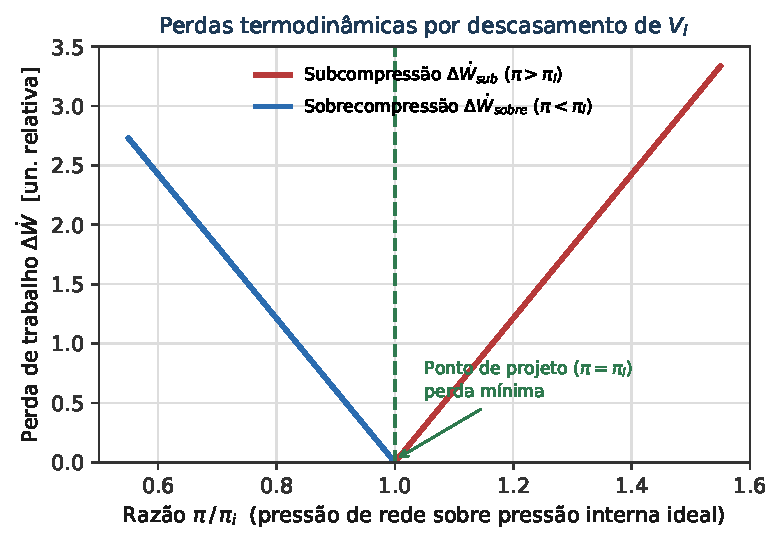
\includegraphics[width=0.60\textwidth]{figuras/fig_5_1_vi_perdas.pdf}
		\caption[Perdas termodinâmicas por sub e sobrecompressão]{Perdas termodinâmicas por sub/sobrecompressão em função do descasamento entre a razão de pressão real e a razão interna ideal do rotor.}
		\label{fig:5-1}
	\end{figure}

	O Gêmeo Digital deve computar continuamente qual regime está ativo comparando $\pi$ medido com $\pi_i$ de projeto, pois essa perda — e não apenas o vazamento por folgas já modelado adiante — é responsável por parte significativa do desvio entre a eficiência isentrópica real e a ideal em condições de operação fora do ponto de projeto (ex.: variação sazonal da contrapressão de rede ou operação em carga parcial).

	\subsection{\textbf{Resfriamento e Separação de Condensado}}
	\begin{itemize}
		\item \textbf{Intercooler e Aftercooler:} Trocadores de calor que removem a energia térmica da compressão. A taxa de calor removido, na Equação~\eqref{eq:s5-10}, segue a forma padrão de projeto de trocadores: coeficiente global de transferência ($U$) vezes área de troca térmica ($A$) vezes a diferença de temperatura média logarítmica ($\Delta T_{\text{LMTD}}$, detalhada no Capítulo de Dinâmica do Intercooler):
		\begin{equation}\label{eq:s5-10}
 \dot{Q} = U \cdot A \cdot \Delta T_{\text{LMTD}}
\end{equation}
		\item \textbf{Drenagem de Condensado:} A umidade removida ($\dot{m}_{\text{cond}}$) é calculada pela variação da razão de umidade $W_h$, na Equação~\eqref{eq:s5-11}:
		\begin{equation}\label{eq:s5-11}
 \dot{m}_{\text{cond}} = \dot{m}_{\text{ar}} \cdot (W_{h,\text{in}} - W_{h,\text{out}}) 
\end{equation}
		\item \textbf{Mecanismo de Falha:} Dreno travado (arraste de água para o estágio seguinte) ou \textit{fouling} (incrustação) no trocador.
		\item \textbf{Detecção:} Sensores de nível capacitivos e queda no coeficiente global de transferência de calor $U$.
	\end{itemize}
	
	\subsection{\textbf{Válvulas de Controle e Segurança}}
	\begin{itemize}
		\item \textbf{Válvula de Retenção (Check Valve):} Impede o fluxo reverso do reservatório para o compressor na parada.
		\item \textbf{Válvula de Alívio (Blow-down):} Despressuriza o sistema interno para permitir a partida em vazio (\textit{unloaded start}).
	\end{itemize}
	
	\subsection{\textbf{Equacionamento Integrado e Balanço de Potência}}
	A potência total consumida pelo sistema, monitorada pelo Gêmeo Digital para detecção de desvios, é a soma das demandas termodinâmicas e perdas mecânicas, dada pela Equação~\eqref{eq:s5-12}:

	\begin{equation}\label{eq:s5-12}
	\dot{W}_{\text{total}} = \underbrace{\dot{W}_{\text{LP}} + \dot{W}_{\text{HP}}}_{\text{Trabalho de Compressão}} + \underbrace{P_{\text{loss,gb}}}_{\text{Perdas na Gearbox}} + \underbrace{\dot{W}_{\text{bomba}}}_{\text{Potência de Lubrificação}} + \underbrace{P_{\text{fric}}}_{\text{Atrito nos Mancais}}
\end{equation}
	
	Onde:
	\begin{itemize}
		\item $\dot{W}_{\text{LP}}$ e $\dot{W}_{\text{HP}}$: Trabalho termodinâmico nos estágios de baixa e alta pressão.
		\item $P_{\text{loss,gb}}$: Perdas por engrenamento e ventilação na caixa multiplicadora.
		\item $\dot{W}_{\text{bomba}}$: Potência consumida pela bomba de óleo lubrificante.
		\item $P_{\text{fric}}$: Perdas mecânicas por atrito viscoso nos rolamentos e selos.
	\end{itemize}
	
	\vspace{1em}
	\textbf{Eficiência Global do Sistema:} A Equação~\eqref{eq:s5-13} compara o trabalho mínimo teórico de uma compressão isotérmica ideal (o limite termodinâmico, sem nenhuma perda) contra o trabalho total realmente consumido pelo trem de potência (Equação~\eqref{eq:s5-12}) — quanto mais próximo de 1, mais perto do ideal termodinâmico a máquina está operando:
	\begin{equation}\label{eq:s5-13}
 \eta_{\text{global}} = \frac{\dot{W}_{\text{isotérmico\_ideal}}}{\dot{W}_{\text{total}}}
\end{equation}

	\subsection{\textbf{Pressão Intermediária Ótima entre Estágios}}
	A Equação~\eqref{eq:s5-5} modela o trabalho de cada estágio isoladamente, mas não responde a uma pergunta de projeto e de diagnóstico igualmente relevante: dada uma pressão de sucção $P_1$ fixa e uma pressão de descarga final $P_2$ fixa, em que pressão intermediária $P_{\text{int}}$ o trabalho total dos dois estágios é mínimo? A resposta é a formulação clássica de compressão multiestágio \cite{cengel, moran, hanlon}, obtida somando a Equação~\eqref{eq:s5-5} para os estágios LP e HP e minimizando o trabalho total em relação a $P_{\text{int}}$: com resfriamento intermediário \textbf{perfeito} (o intercooler devolve o ar à mesma temperatura de sucção do estágio LP, $T_{HP,\text{in}} = T_{LP,\text{in}}$) e mesmo índice politrópico $n$ nos dois estágios, o mínimo ocorre exatamente quando as duas razões de pressão são iguais — condição que se resolve na média geométrica das pressões extremas, pela Equação~\eqref{eq:s5-14}:
	\begin{equation}\label{eq:s5-14}
 P_{\text{int}}^{*} = \sqrt{P_1 \cdot P_2}
\end{equation}
	Nesse ponto ótimo, $P_{\text{int}}^{*}$ nada mais é do que a pressão interestágio já instrumentada na matriz do Capítulo 18 — a descarga do estágio LP e a sucção do estágio HP são o mesmo ponto físico, $P_{d,lp} = P_{s,hp}$ (ponto C/D da Tabela~\ref{tab:18-1}) — de modo que a Equação~\eqref{eq:s5-14} não introduz variável nova a instrumentar, apenas um valor de referência contra o qual comparar a leitura existente.

	Na prática, o resfriamento intermediário nunca é perfeito: o intercooler degradado modelado pela Equação~\eqref{eq:s10-5} (queda de $U$ por incrustação) entrega o ar ao estágio HP mais quente do que o projeto original previa ($T_{HP,\text{in}} > T_{LP,\text{in}}$). Isso encarece relativamente o trabalho do estágio HP para qualquer razão de pressão fixada nele — a mesma física da penalidade térmica já quantificada na Equação~\eqref{eq:s10-4} — e desloca o ponto de mínimo para longe da média geométrica simples da Equação~\eqref{eq:s5-14}. O Gêmeo Digital ganha, com isso, um critério adicional e independente de desvio: comparar a pressão interestágio efetivamente operada contra $P_{\text{int}}^{*}$ não diagnostica apenas um estágio isoladamente, mas se a \textbf{alocação de carga} entre LP e HP ainda corresponde ao ponto de projeto de fábrica — um sintoma que nenhum dos dois estágios, olhado sozinho, revela.

	\subsection{\textbf{Perda de Carga na Tubulação Interestágios}}
	Todo o equacionamento deste capítulo até aqui trata $P_{\text{int}}$ como um único valor, comum à descarga do estágio LP, à entrada e à saída do intercooler e à sucção do estágio HP — como se os trechos de tubulação que interligam esses pontos não impusessem queda de pressão própria. Essa simplificação ignora o atrito distribuído do escoamento contra a parede do tubo, mecanismo distinto da perda localizada já modelada para filtro e silenciador (Equação~\eqref{eq:s5-4}): ali a perda vem de uma restrição concentrada num único elemento; aqui vem do comprimento inteiro da linha. A forma clássica de Darcy-Weisbach isola essa diferença mantendo a mesma pressão dinâmica $\rho v^2/2$ já usada na Equação~\eqref{eq:s5-4}, agora multiplicada pela razão comprimento/diâmetro da linha em vez de um coeficiente de perda localizada \cite{white} — Equação~\eqref{eq:s5-15}:
	\begin{equation}\label{eq:s5-15}
 \Delta P_{\text{linha}} = f_D \cdot \frac{L_{\text{linha}}}{D_{\text{linha}}} \cdot \frac{\rho \, v^2}{2}
\end{equation}
	Onde $f_D$ é o fator de atrito de Darcy (função do número de Reynolds e da rugosidade relativa da tubulação \cite{white}), $L_{\text{linha}}$ o comprimento do trecho e $D_{\text{linha}}$ seu diâmetro interno. Cada trecho interestágios (descarga LP$\to$intercooler, intercooler$\to$sucção HP, descarga HP$\to$aftercooler) tem sua própria Equação~\eqref{eq:s5-15}, com $f_D$, $L_{\text{linha}}$ e $D_{\text{linha}}$ específicos daquele trecho. O efeito prático é uma pequena correção à pressão usada nas Equações~\eqref{eq:s5-5}, \eqref{eq:s5-8}/\eqref{eq:s5-9} e~\eqref{eq:s5-14}: a pressão de sucção do estágio seguinte é a pressão de descarga do estágio anterior \textbf{menos} a Equação~\eqref{eq:s5-15} do trecho que os liga, não o mesmo valor de $P_{\text{int}}$ usado até aqui por simplificação. Em linhas curtas e bem dimensionadas dentro do próprio pacote (\textit{skid}), essa correção costuma ser pequena frente às demais perdas do capítulo — mas cresce com o desgaste (rugosidade interna por corrosão/incrustação, que eleva $f_D$ ao longo da vida da instalação) e deve ser tratada como mais um sintoma rastreável pelo Gêmeo Digital, não descartada por ser pequena no comissionamento.

	\subsection{\textbf{Perda de Carga Parametrizada em Válvulas de Alívio e Retenção}}

	O catálogo de mecanismos de falha do Capítulo 28 (Seção~28.3) trata a válvula de \textit{blow-off}, a válvula de retenção (\textit{check valve}) e a válvula de segurança e alívio (PSV) como mecanismos \textbf{binários}: a válvula funciona dentro da especificação ou falhou (trava aberta, trava fechada, vaza acima do assento). Essa simplificação deixa de fora o regime intermediário que, na prática, costuma preceder a falha binária — o assento desgasta, a mola perde rigidez por fadiga ou corrosão, ou depósitos se acumulam na sede, e a perda de carga que a válvula impõe ao escoamento cresce de forma gradual muito antes de qualquer travamento. É o mesmo padrão de degradação já modelado para o filtro de admissão (Equação~\eqref{eq:s5-4}) e para a tubulação interestágios (Equação~\eqref{eq:s5-15}) — e a mesma forma clássica de perda de carga localizada se aplica, com um coeficiente próprio de cada válvula, $\zeta_{\text{valv}}$, na Equação~\eqref{eq:s5-16}:

	\begin{equation}\label{eq:s5-16}
	\Delta P_{\text{valv}} = \zeta_{\text{valv}} \cdot \frac{\rho \, v^2}{2}
	\end{equation}

	Como no filtro (Equação~\eqref{eq:s5-4}), $\zeta_{\text{valv}}$ cresce a partir de um valor de referência limpo/novo ($\zeta_{\text{valv,ref}}$) conforme a válvula degrada — mas, diferente do filtro, cuja perda é permanentemente exposta ao escoamento principal, cada válvula deste grupo só é atravessada por vazão em condições específicas (a PSV só abre acima da pressão de ajuste; a de retenção conduz continuamente, mas em um único sentido; o \textit{blow-off} só atua durante alívio de partida ou parada). O sinal de degradação, portanto, não é uma leitura contínua como $\Delta P_{ic}$ do intercooler (ponto D da Tabela~\ref{tab:18-1}), mas o desvio entre a perda de carga observada no instante em que a válvula efetivamente conduz e o valor de referência esperado para aquela vazão — exigindo, tal qual $\zeta_{\text{ref}}$ do filtro (Seção~28.2), um canal de medição de pressão diferencial dedicado, hoje ausente da matriz da Tabela~\ref{tab:18-1}.

	Com esse coeficiente definido, a mesma técnica de estimação conjunta de estado e parâmetro que identifica $K$, $\eta_{\text{mec}}$ e $\zeta_{\text{ref}}$ (Seção~28.1) se estende naturalmente a $\zeta_{\text{valv}}$: basta incluí-lo no vetor $\Lambda$ da Equação~\eqref{eq:s28-1}, desde que exista, para aquela válvula específica, a medição de $\Delta P_{\text{valv}}$ que torna o parâmetro observável — a mesma condição discutida na Seção de Condição de Observabilidade do Capítulo 21, agora aplicada a um quarto parâmetro estático em vez dos três originais.

	\vspace{1em}
	\hrule
	\vspace{1em}

	\textbf{Diretriz Técnica Final:} A Equação~\eqref{eq:s5-13} consolida todo o capítulo em um único KPI de eficiência global — mas seu valor só é confiável se cada termo de perda (folga interna via $V_i$, gearbox, bomba de óleo) estiver sendo medido ou estimado corretamente; um $\eta_{\text{global}}$ isolado sem essa rastreabilidade componente-a-componente é apenas um número, não um diagnóstico. A Equação~\eqref{eq:s5-14} acrescenta um segundo eixo de leitura, ortogonal ao primeiro: mesmo com $\eta_{\text{global}}$ nominal, uma pressão interestágio deslocada do ótimo indica que a carga entre os dois estágios está mal balanceada — tipicamente o primeiro sinal observável de um intercooler em degradação, antes mesmo que a Equação~\eqref{eq:s10-4} feche o diagnóstico. A Equação~\eqref{eq:s5-15} fecha a última lacuna de perda de carga do trem primário: uma tendência de alta em $f_D$ para o mesmo ponto de operação, isolada da leitura de $P_{\text{int}}$, é sintoma de degradação da própria tubulação (corrosão, incrustação interna), independente de qualquer coisa que esteja acontecendo no intercooler ou nos estágios. A Equação~\eqref{eq:s5-16} estende essa mesma lógica de perda de carga localizada às válvulas de alívio e retenção, hoje tratadas como falha binária no catálogo do Capítulo 28 — uma tendência de alta em $\zeta_{\text{valv}}$ é o análogo, para essas válvulas, do que a tendência de alta em $\zeta_{\text{ref}}$ já representa para o filtro de admissão.

	% --- Fim do Capítulo 5 ---
	
	% --- Início do Capítulo 6: Engenharia do Trem de Transmissão e Matriz de Confiabilidade ---
	
	\clearpage
	\section{\textbf{Engenharia do Trem de Transmissão e Matriz de Confiabilidade}}
	
	Este capítulo detalha a modelagem física do sistema de transmissão de potência, integrando a cinemática da caixa multiplicadora com a dinâmica de falhas mecânicas. O objetivo é estabelecer o modelo de referência para o Gêmeo Digital, permitindo o isolamento entre perdas mecânicas e termodinâmicas.
	
	\subsection{\textbf{Cinemática e Fluxo de Potência}}
	A transferência de energia do motor para os rotores de compressão (LP e HP) é governada pela conservação do momento angular e pelas eficiências de interface.
	\begin{itemize}
		\item \textbf{Balanço de Potência Instantânea:} A Equação~\eqref{eq:s6-1} afirma que toda a potência entregue pelo motor (já descontada a perda no acoplamento) é distribuída entre o trabalho de compressão nos dois estágios ($P_{\text{LP}}$, $P_{\text{HP}}$), as perdas da gearbox e um termo de aceleração angular do sistema — este último relevante apenas em transientes, pois some quando a rotação é constante ($d\omega/dt = 0$):
		\begin{equation}\label{eq:s6-1}
 P_{\text{mot}} \cdot \eta_{\text{acopl}} = P_{\text{LP}} + P_{\text{HP}} + P_{\text{loss,gb}} + I_{\text{sys}} \cdot \omega \cdot \frac{d\omega}{dt}
\end{equation}
		Onde $P_{\text{loss,gb}}$ é a potência dissipada na caixa multiplicadora e $I_{\text{sys}}$ é o momento de inércia equivalente referido ao eixo do motor.
		\item \textbf{Relação de Transmissão e Velocidades:} A razão de engrenamento entre coroa e pinhão eleva a rotação do motor até a velocidade de operação dos rotores, conforme a Equação~\eqref{eq:s6-2}:
		\begin{equation}\label{eq:s6-2}
 \omega_{\text{rotor}} = \omega_{\text{mot}} \cdot \frac{Z_{\text{coroa}}}{Z_{\text{pinhão}}} 
\end{equation}
	\end{itemize}
	
	\subsection{\textbf{Modelagem de Perdas Parasitas na Gearbox}}
	As perdas na caixa multiplicadora variam dinamicamente com a carga, rotação e viscosidade do óleo $\mu(T)$.
	\begin{itemize}
		\item \textbf{Perdas por Engrenamento ($P_{\text{mesh}}$):} A Equação~\eqref{eq:s6-3} modela a fração da potência transmitida ($P_{\text{trans}}$) que se converte em atrito no contato entre os dentes, escalada pelo coeficiente de atrito e por um termo geométrico dependente do ângulo de pressão da engrenagem:
		\begin{equation}\label{eq:s6-3}
 P_{\text{mesh}} = f_{\text{fric}} \cdot P_{\text{trans}} \cdot \cos^{-1}(\phi)
\end{equation}
		Onde $f_{\text{fric}}$ é o coeficiente de atrito (função da rugosidade e lubrificação) e $\phi$ é o ângulo de pressão.
		\item \textbf{Perdas por Agitação e Ventilação ($P_{\text{windage}}$):} O arrasto viscoso do óleo contra as engrenagens em rotação cresce com o cubo da velocidade angular, pela Equação~\eqref{eq:s6-4}:
		\begin{equation}\label{eq:s6-4}
 P_{\text{windage}} = C_w \cdot \rho_{\text{óleo}} \cdot \omega^3 \cdot D^5 
\end{equation}
		Onde $C_w$ é o coeficiente de arrasto e $D$ o diâmetro das engrenagens.
	\end{itemize}
	
	\subsection{\textbf{Matriz de Mecanismos de Falha e Indicadores Digitais}}
	A Tabela~\ref{tab:6-1} correlaciona cada componente físico da caixa multiplicadora ao seu modo de falha característico e ao indicador digital que permite detectá-lo. A leitura é por linha: o componente identifica \textit{onde} a falha ocorre; o mecanismo descreve \textit{como} ela progride fisicamente; e o indicador digital é a grandeza — medida ou inferida — cujo desvio denuncia a progressão antes que ela atinja o limite funcional. Essa estrutura de três colunas se repete nas matrizes de falha dos capítulos seguintes, e é o que permite ao Gêmeo Digital passar de um diagnóstico genérico (``vibração alta'') para uma hipótese de causa raiz específica.
	
	\begin{table}[h!tbp]
		\centering
		\resizebox{\textwidth}{!}{
		\begin{tabular}{l l l l}
			\toprule
			\textbf{Componente} & \textbf{Mecanismo de Falha} & \textbf{Causa Raiz} & \textbf{Indicador Digital} \\ \midrule
			Acoplamento & Desalinhamento & Assentamento / Térmico & Pico em $2 \times \text{RPM}$ \\
			Acoplamento & Fadiga do Elemento & Sobrecarga & Resíduo de torque $r_{\tau}$ \\
			Engrenagens & \textit{Pitting} (Fadiga) & Carga cíclica & Bandas laterais em $GMF$ \\
			Engrenagens & \textit{Scuffing} & Falha de filme de óleo & $\uparrow T$ óleo de retorno \\
			Mancais & Desgaste de Metal & Contaminação & $\downarrow P_{\text{óleo}}$ e vibração \\
			Selos & Desgaste Labirinto & Vibração excessiva & $\downarrow \eta_{\text{vol}}$ e $\uparrow T_{\text{suc}}$ \\ \bottomrule
		\end{tabular}
		}
		\caption[Mecanismos de falha da caixa multiplicadora]{Mecanismos de falha do acoplamento, engrenagens, mancais e selos da caixa multiplicadora, com o respectivo indicador digital monitorado pelo Gêmeo Digital.}
		\label{tab:6-1}
	\end{table}
	
	\subsection{\textbf{Dinâmica de Eixos e Sincronismo (Timing)}}
	Em compressores isentos de óleo, as engrenagens de sincronismo garantem que os rotores mantenham a folga nominal sem contato físico.
	\begin{itemize}
		\item \textbf{Rigidez Torcional do Eixo ($k_t$):} A Equação~\eqref{eq:s6-5} estima a torção angular ($\Delta \theta$) que o eixo sofre ao transmitir um torque $\tau$ ao longo de um comprimento $L$, em função da rigidez do material — módulo de cisalhamento $G$ e momento polar de inércia da seção transversal $J$ (ambos parâmetros geométricos/de material fixos do eixo):
		\begin{equation}\label{eq:s6-5}
 \Delta \theta = \frac{\tau \cdot L}{G \cdot J}
\end{equation}
		\item \textbf{Risco Crítico:} Se $\Delta \theta$ exceder o \textit{backlash} de projeto, ocorre contato metal-metal. O Gêmeo Digital detecta isso via \textit{Motor Current Signature Analysis} (MCSA).
	\end{itemize}
	
	\subsection{\textbf{Diagnóstico por Resíduos de Potência}}
	O Gêmeo Digital calcula o resíduo mecânico ($r_{\text{mec}}$) para isolar anomalias, pela Equação~\eqref{eq:s6-6}:
	\begin{equation}\label{eq:s6-6}
 r_{\text{mec}} = P_{\text{real}} - \left( \frac{\dot{W}_{\text{LP}} + \dot{W}_{\text{HP}}}{\eta_{\text{mec,modelo}}} \right) 
\end{equation}
	\begin{itemize}
		\item $r_{\text{mec}} > 0$: Indica aumento de atrito (falha de rolamento ou engrenagem).
		\item $r_{\text{mec}} < 0$: Indica erro de calibração ou fuga interna massiva.
	\end{itemize}
	
	\subsection{\textbf{Frequências de Monitoramento}}
	As frequências características usadas ao longo deste documento como referência de diagnóstico espectral seguem diretamente da cinemática do trem de potência — a Equação~\eqref{eq:s6-7} converte a rotação medida (RPM) na frequência de giro do eixo ($f_r$) e, a partir dela, na frequência de engrenamento ($GMF$, aqui $f_g$) pelo número de dentes $Z$:
	\begin{equation}\label{eq:s6-7}
 f_r = \frac{\text{RPM}}{60} \quad ; \quad f_g = f_r \cdot Z
\end{equation}

	\vspace{1em}
	\textbf{Equação de Torque de Referência:} A Equação~\eqref{eq:s6-8} sintetiza tudo o que foi apresentado neste capítulo em um único torque teórico esperado no eixo do motor: soma o trabalho politrópico de compressão dos dois estágios (LP e HP) com as perdas da gearbox, e converte de potência para torque dividindo pela rotação do motor e pela eficiência da caixa multiplicadora — este é o valor de referência contra o qual o torque real medido é comparado no resíduo mecânico $r_{\text{mec}}$ da Equação~\eqref{eq:s6-6}:
	\begin{equation}\label{eq:s6-8}
 \boxed{\tau_{\text{ref}} = \frac{1}{\omega_{\text{mot}} \cdot \eta_{\text{gb}}} \left[ \sum_{i=1}^{2} \left( \frac{n}{n-1} P_{\text{in},i} \dot{V}_{\text{in},i} \left( \pi_i^{\frac{n-1}{n}} - 1 \right) \right) + P_{\text{loss,gb}} \right]}
\end{equation}

	\vspace{1em}
	\hrule
	\vspace{1em}

	\textbf{Diretriz Técnica Final:} O torque de referência da Equação~\eqref{eq:s6-8} é o valor teórico esperado a partir das condições de processo; o resíduo mecânico ($r_{\text{mec}}$) desta seção só é um diagnóstico útil se comparado continuamente contra esse torque de referência recalculado em tempo real — nunca contra um valor de projeto fixo.

	% --- Fim do Capítulo 6 ---
	
	% --- Início do Capítulo 7: Sistema de Lubrificação e Dinâmica de Mancais (Versão Expandida) ---
	
	\clearpage
	\section{\textbf{Sistema de Lubrificação, Arrefecimento de Óleo e Dinâmica de Mancais}}
	
	Este capítulo detalha a modelagem do sistema de suporte vital dos componentes rotativos. Em compressores isentos de óleo, o lubrificante é responsável pela integridade da caixa multiplicadora e dos mancais de alta rotação, atuando como o principal meio de transporte de calor dissipado por atrito mecânico.
	
	\subsection{\textbf{Acionamento e Consumo Energético da Bomba de Óleo}}
	O sistema utiliza uma bomba de deslocamento positivo acionada por um motor elétrico independente, permitindo as funções críticas de pré-lubrificação e pós-lubrificação (\textit{standby cooling}).
	\begin{itemize}
		\item \textbf{Potência Elétrica Consumida ($P_{\text{elec,pump}}$):} A Equação~\eqref{eq:s7-1} iguala duas formas de calcular a mesma potência — o lado elétrico (tensão $V$, corrente $I$ e fator de potência $\cos\phi$ trifásicos, medidos no painel) e o lado hidráulico (vazão de óleo vezes o diferencial de pressão da bomba, dividido pela eficiência total). Comparar os dois lados é justamente o que permite detectar falha antes que ela se manifeste mecanicamente:
		\begin{equation}\label{eq:s7-1}
 P_{\text{elec,pump}} = \sqrt{3} \cdot V \cdot I \cdot \cos \phi = \frac{\dot{V}_{\text{oil}} \cdot \Delta P_{\text{pump}}}{\eta_{\text{total,pump}}}
\end{equation}
		\item \textbf{Indicador de Saúde:} O Gêmeo Digital monitora o desvio de corrente $\Delta I = I_{\text{medido}} - I_{\text{modelo}}(T_{\text{oil}})$. Um aumento em $\Delta I$ sem aumento de pressão indica falha iminente no enrolamento do motor ou travamento mecânico da bomba.
	\end{itemize}
	
	\subsection{\textbf{Reologia do Lubrificante e Perda de Carga no Circuito}}
	A viscosidade dinâmica $\mu(T)$ é o parâmetro central para o cálculo de perdas e proteção de película.
	\begin{itemize}
		\item \textbf{Equação de Vogel \cite{vogel} para Viscosidade:} A Equação~\eqref{eq:s7-2} descreve a queda não linear da viscosidade dinâmica com a temperatura:
		\begin{equation}\label{eq:s7-2}
 \mu(T) = a \cdot \exp \left( \frac{b}{T - c} \right) 
\end{equation}
		Onde $a$, $b$ e $c$ são constantes empíricas obtidas por ajuste de curva aos dados do fabricante do lubrificante (não possuem significado físico individual — apenas a combinação reproduz a curva $\mu \times T$ medida). A Figura~\ref{fig:7-1} ilustra a forma típica dessa curva: a viscosidade cai de forma acentuadamente não linear com o aumento da temperatura, e é justamente essa não linearidade que torna a Equação~\eqref{eq:s7-2} necessária em vez de uma simples interpolação linear.

		\begin{figure}[h!tbp]
			\centering
			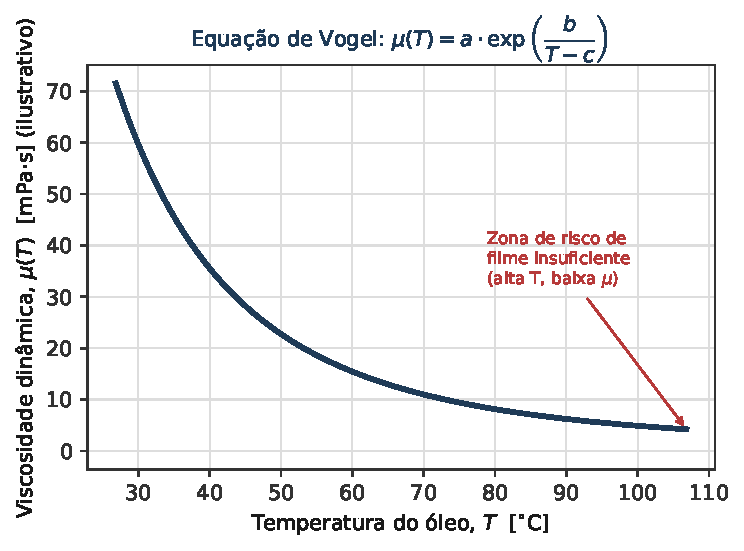
\includegraphics[width=0.60\textwidth]{figuras/fig_7_1_vogel.pdf}
			\caption[Curva de viscosidade de Vogel]{Curva de viscosidade de Vogel — queda não linear da viscosidade com a temperatura (valores ilustrativos).}
			\label{fig:7-1}
		\end{figure}

		\item \textbf{Perda de Carga no Filtro ($\Delta P_{\text{filt}}$):} Modelada pela lei de Darcy-Forchheimer para meios porosos, na Equação~\eqref{eq:s7-3}:
		\begin{equation}\label{eq:s7-3}
 \Delta P_{\text{filt}} = \underbrace{A \cdot \mu \cdot v}_{\text{Componente Viscosa}} + \underbrace{B \cdot \rho \cdot v^2}_{\text{Componente Inercial}} 
\end{equation}
		Onde $A$ e $B$ são coeficientes de permeabilidade e inércia do elemento filtrante.
	\end{itemize}
	
	\subsection{\textbf{Dinâmica de Mancais e Balanço Térmico}}
	Os mancais de alta rotação dissipam energia por cisalhamento viscoso, elevando a temperatura do óleo.
	\begin{itemize}
		\item \textbf{Potência de Atrito nos Mancais ($P_{\text{fric,brg}}$):} A Equação~\eqref{eq:s7-4} descreve a dissipação viscosa dentro do filme de óleo do mancal: cresce com a viscosidade $\mu$, com o quadrado da velocidade angular $\omega$, com o cubo do raio do mancal $R$ e com o comprimento axial $L$, mas é inversamente proporcional à espessura do filme lubrificante $e_{\text{filme}}$ — um filme mais fino dissipa mais energia por atrito, com $\xi$ como coeficiente de forma do mancal:
		\begin{equation}\label{eq:s7-4}
 P_{\text{fric,brg}} = \xi \cdot \frac{\mu \cdot \omega^2 \cdot R^3 \cdot L}{e_{\text{filme}}}
\end{equation}
		Onde $e_{\text{filme}}$ é a espessura da película lubrificante (usa-se $e_{\text{filme}}$ em vez de $h$ para não colidir com a entalpia específica dos capítulos de termodinâmica).
		\item \textbf{Elevação de Temperatura do Óleo ($\Delta T_{\text{oil}}$):} A Equação~\eqref{eq:s7-5} converte a potência de atrito total num aumento de temperatura, via vazão mássica e calor específico do óleo:
		\begin{equation}\label{eq:s7-5}
 \Delta T_{\text{oil}} = \frac{P_{\text{fric,total}}}{\dot{m}_{\text{oil}} \cdot c_{p,\text{oil}}} 
\end{equation}
		O Gêmeo Digital utiliza este balanço para validar se o fluxo de óleo ($\dot{m}_{\text{oil}}$) está adequado para a carga térmica atual.
	\end{itemize}
	
	\subsection{\textbf{Gerenciamento Térmico e Válvula Termostática}}
	O controle da temperatura é realizado via trocador de calor e uma válvula termostática de três vias.
	\begin{itemize}
		\item \textbf{Efetividade do Resfriador ($\epsilon$):} A Equação~\eqref{eq:s7-6} mede quanto da queda de temperatura teoricamente possível o resfriador realmente entrega — a razão entre a queda real do óleo ($T_{\text{oil,in}} - T_{\text{oil,out}}$) e a máxima queda termodinamicamente possível, limitada pela temperatura de entrada da água de resfriamento ($T_{\text{oil,in}} - T_{\text{water,in}}$):
		\begin{equation}\label{eq:s7-6}
 \epsilon = \frac{T_{\text{oil,in}} - T_{\text{oil,out}}}{T_{\text{oil,in}} - T_{\text{water,in}}}
\end{equation}
		\item \textbf{Lógica da Válvula Termostática:} O modelo prevê a posição da válvula baseada no \textit{setpoint} de operação. Se $T_{\text{oil}}$ sobe e a válvula está 100\% aberta para o resfriador sem queda de temperatura, o modelo identifica \textit{fouling} (incrustação) no trocador.
	\end{itemize}
	
	\subsection{\textbf{Matriz de Mecanismos de Falha do Sistema de Óleo}}
	A Tabela~\ref{tab:7-1} associa cada componente do circuito de lubrificação ao seu modo de falha típico e ao indicador digital correspondente, usado pelo Gêmeo Digital para diagnóstico automático.
	\begin{table}[h!tbp]
		\centering
		\small
		\renewcommand{\arraystretch}{1.5}
		\begin{tabular}{l l l}
			\toprule
			\textbf{Componente} & \textbf{Mecanismo de Falha} & \textbf{Indicador no Gêmeo Digital} \\ \midrule
			\textbf{Motor da Bomba} & Sobrecarga / Curto-circuito & $\uparrow I_{\text{pump}}$ (Resíduo de Corrente) \\
			\textbf{Bomba de Óleo} & Cavitação ou Desgaste & $\downarrow P_{\text{oil}}$ vs $\uparrow \text{RPM}$ da Bomba \\
			\textbf{Filtro de Óleo} & Colmatagem (Saturação) & $\uparrow \Delta P_{\text{filt}}$ (Normalizado pela viscosidade) \\
			\textbf{Resfriador} & Incrustação (\textit{Fouling}) & $\downarrow \epsilon$ (Queda na Efetividade Térmica) \\
			\textbf{Mancais} & Desgaste de Metal Patente & $\uparrow T_{\text{brg}}$ e $\uparrow$ Vibração de Alta Frequência \\ \bottomrule
		\end{tabular}
		\caption[Mecanismos de falha do sistema de lubrificação]{Matriz de mecanismos de falha do sistema de lubrificação (bomba, filtro, resfriador e mancais).}
		\label{tab:7-1}
	\end{table}
	
	\subsection{\textbf{Equacionamento de Diagnóstico por Resíduos}}
	O isolamento de falhas é realizado através do cálculo de resíduos em tempo real:
	\begin{itemize}
		\item \textbf{Resíduo de Pressão ($r_{\Delta P}$):} $ \Delta P_{\text{real}} - \Delta P_{\text{modelo}}(\dot{V}, \mu) $
		\item \textbf{Resíduo de Potência da Bomba ($r_{P}$):} $ P_{\text{elec,medido}} - P_{\text{hidráulico,calc}} $
		\item \textbf{Resíduo Térmico ($r_{\epsilon}$):} $ \epsilon_{\text{real}} - \epsilon_{\text{modelo}} $
	\end{itemize}
	
	\vspace{1em}
	\textbf{Estado de Saúde do Sistema de Óleo ($SOH_{\text{oil}}$):} A Equação~\eqref{eq:s7-7} consolida três razões normalizadas — viscosidade real sobre nominal, limite de perda de carga sobre perda real no filtro, e efetividade real sobre nominal do resfriador — cada uma variando entre 0 (crítico) e 1 (saudável), e toma o menor valor entre as três como saúde global do sistema:
	\begin{equation}\label{eq:s7-7}
 \boxed{SOH_{\text{oil}} = \min \left( \frac{\mu_{\text{real}}}{\mu_{\text{nom}}}, \frac{\Delta P_{\text{lim}}}{\Delta P_{\text{real}}}, \frac{\epsilon_{\text{real}}}{\epsilon_{\text{nom}}} \right)}
\end{equation}

	\subsection{\textbf{Análise Físico-Química do Óleo (Canal Laboratorial \textit{Offline})}}
	As três entradas da Equação~\eqref{eq:s7-7} — viscosidade, perda de carga e efetividade térmica — têm em comum o fato de serem todas medidas \textbf{online}, em tempo real, por sensores permanentes de campo. Esse canal é rápido, mas cego a um tipo de degradação: a deterioração química do próprio óleo, que só se manifesta na viscosidade ou no $\Delta P$ depois de já ter avançado o suficiente para alterar as propriedades físicas do fluido. A prática consolidada de manutenção preditiva \cite{mobley} complementa o monitoramento online com uma tríade laboratorial \textbf{offline}, amostrada periodicamente:
	\begin{itemize}
		\item \textbf{Número de Acidez Total (TAN):} Medido por titulação potenciométrica \cite{astmd664}, quantifica os subprodutos ácidos da oxidação do óleo em serviço. Uma tendência de alta do TAN antecede a queda de viscosidade e a formação de vernizes/borras que eventualmente entopem o filtro — é o primeiro sinal químico de que o óleo está no fim da vida útil, ainda quando $SOH_{\text{oil}}$ da Equação~\eqref{eq:s7-7} continua em 1.
		\item \textbf{Água no Óleo:} Medida por titulação coulométrica de Karl Fischer \cite{astmd6304}, quantifica a contaminação por umidade — relevante mesmo em circuito fechado, pois condensação interna (partida a frio, variação de temperatura ambiente offshore) introduz água sem qualquer falha de vedação externa. Água dissolvida acelera a própria oxidação que o TAN mede, tornando os dois ensaios complementares, não redundantes.
		\item \textbf{Contagem de Partículas (Código ISO 4406):} Reporta a concentração de partículas sólidas em três faixas de tamanho ($\ge 4\,\mu\text{m}$, $\ge 6\,\mu\text{m}$, $\ge 14\,\mu\text{m}$) como um código de três números \cite{iso4406}. É o canal que detecta desgaste abrasivo incipiente de engrenagens e rolamentos — partículas metálicas no óleo — antes que esse desgaste produza qualquer assinatura vibracional detectável pelos acelerômetros já instrumentados no ponto B da Tabela~\ref{tab:18-1}.
	\end{itemize}
	Os três ensaios entram no Gêmeo Digital como tendências de baixa frequência (tipicamente uma amostra a cada troca programada ou intervalo fixo, não em tempo real), alimentando o mesmo princípio de variável \textit{real} versus \textit{virtual} já estabelecido na matriz do Capítulo 18 — mas como uma terceira categoria, intermediária entre as duas: medição real, porém de baixíssima taxa de amostragem, o que exige do modelo uma lógica de interpolação/extrapolação de tendência distinta da usada para os sensores contínuos.

	\vspace{1em}
	\hrule
	\vspace{1em}

	\textbf{Diretriz Técnica Final:} O uso do operador $\min(\cdot)$ na Equação~\eqref{eq:s7-7} é deliberado — o Estado de Saúde do sistema de óleo é sempre ditado pelo pior indicador entre viscosidade, perda de carga e efetividade térmica, nunca por uma média entre eles, refletindo que uma única falha isolada já compromete a lubrificação como um todo. A tríade laboratorial desta seção não substitui $SOH_{\text{oil}}$ — ela o antecede: TAN, água e contagem de partículas tipicamente sinalizam degradação química e desgaste abrasivo semanas ou meses antes que a Equação~\eqref{eq:s7-7} caia, porque medem a causa quando o canal online ainda só vê o efeito.

	% --- Fim do Capítulo 7 ---
	
	% --- Início do Capítulo 8: Dinâmica de Transmissão e Sincronismo (Versão Integral) ---
	
	\clearpage
	\section{\textbf{Dinâmica de Transmissão, Sincronismo e Integridade de Engrenamentos}}
	
	Este capítulo detalha a modelagem física da transmissão de potência em compressores de múltiplos estágios, focando na cinemática de engrenamento, na integridade estrutural dos dentes, na dinâmica de rolamentos de precisão e nos efeitos de desalinhamento.
	
	\subsection{\textbf{Cinemática da Transmissão e Relações de Velocidade}}
	Em uma configuração de motor único com caixa integrada, a coroa principal (\textit{Bull Gear}) aciona simultaneamente os pinhões dos estágios de Baixa Pressão (LP) e Alta Pressão (HP). O sincronismo interno de cada par de rotores é garantido por engrenagens de \textit{timing} dedicadas. A Figura~\ref{fig:8-1} esquematiza essa cinemática: a coroa central, acionada pelo motor, engrena simultaneamente com os dois pinhões (LP e HP), cada um girando a uma velocidade diferente conforme sua própria relação de dentes — exatamente a lógica capturada pela Equação~\eqref{eq:s8-1} a seguir.

	\begin{figure}[h!tbp]
		\centering
		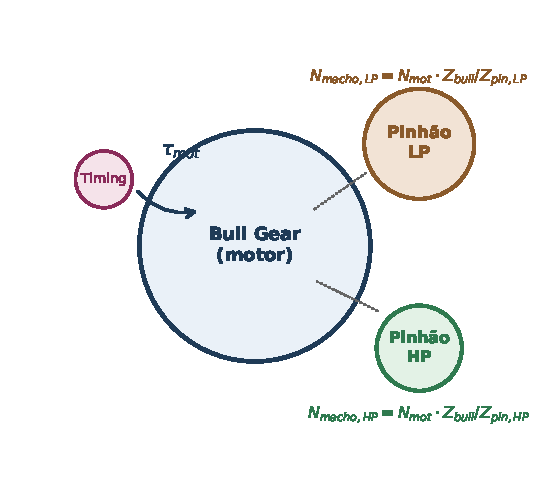
\includegraphics[width=0.75\textwidth]{figuras/fig_8_1_gearbox.pdf}
		\caption[Esquema cinemático da caixa multiplicadora]{Esquema cinemático simplificado da caixa multiplicadora: coroa (\textit{bull gear}) acionando os pinhões LP e HP, com engrenagem de sincronismo (\textit{timing}).}
		\label{fig:8-1}
	\end{figure}

	\begin{itemize}
		\item \textbf{Relação de Multiplicação dos Estágios ($i$):}
		A rotação do rotor macho de cada estágio ($N_{\text{macho}}$) é determinada pela geometria da \textit{gearbox}:
		\begin{equation}\label{eq:s8-1}
 N_{\text{macho,LP}} = N_{\text{mot}} \cdot \left( \frac{Z_{\text{bull}}}{Z_{\text{pin,LP}}} \right) \quad ; \quad N_{\text{macho,HP}} = N_{\text{mot}} \cdot \left( \frac{Z_{\text{bull}}}{Z_{\text{pin,HP}}} \right) 
\end{equation}
		Onde $Z_{\text{bull}}$ é o número de dentes da coroa e $Z_{\text{pin}}$ o do pinhão.
		
		\item \textbf{Sincronismo Interno (Relação Macho-Fêmea):}
		As engrenagens de sincronismo (\textit{timing gears}) impõem a relação de velocidades necessária para evitar o contato entre os lóbulos, pela Equação~\eqref{eq:s8-2}:
		\begin{equation}\label{eq:s8-2}
 N_{\text{fêmea}} = N_{\text{macho}} \cdot \left( \frac{Z_{\text{sync,macho}}}{Z_{\text{sync,fêmea}}} \right) 
\end{equation}
		O Gêmeo Digital monitora o erro de fase angular $\Delta \phi = \theta_{\text{macho}} - G_s \theta_{\text{fêmea}}$ para prever colisões.
	\end{itemize}
	
	\subsection{\textbf{Equacionamento de Torque e Balanço de Potência}}
	O torque total fornecido pelo motor ($\tau_{\text{mot}}$) é distribuído entre os estágios, considerando as eficiências de engrenamento ($\eta_{\text{gb}}$).
	\begin{itemize}
		\item \textbf{Balanço de Torque no Eixo da Coroa:} A Equação~\eqref{eq:s8-3} reparte o torque do motor (já descontada a eficiência de engrenamento $\eta_{\text{gb}}$) entre os dois pinhões, cada torque de estágio dividido pela sua respectiva relação de transmissão ($i_{\text{LP}}$, $i_{\text{HP}}$):
		\begin{equation}\label{eq:s8-3}
 \tau_{\text{mot}} \cdot \eta_{\text{gb}} = \frac{\tau_{\text{LP}}}{i_{\text{LP}}} + \frac{\tau_{\text{HP}}}{i_{\text{HP}}}
\end{equation}
		Onde $\tau_{\text{LP}}$ e $\tau_{\text{HP}}$ são os torques requeridos pela compressão. Desvios neste balanço indicam anomalias mecânicas (ex: atrito excessivo em selos) ou depósitos nos rotores.
	\end{itemize}
	
	\subsection{\textbf{Dinâmica de Rolamentos e Diagnóstico de Vida Útil}}
	Os pinhões de alta velocidade são suportados por rolamentos de precisão, cuja vida útil nominal ($L_{10h}$) é modelada em função da carga equivalente $P$:
	\begin{itemize}
		\item \textbf{Carga Equivalente e Vida Útil:} A Equação~\eqref{eq:s8-4} combina as cargas radial e axial reais em uma única carga equivalente $P$ (norma ISO 281), e usa essa carga equivalente para projetar quantas horas de operação o rolamento suporta antes de 10\% da população falhar por fadiga:
		\begin{equation}\label{eq:s8-4}
 P = X \cdot F_r + Y \cdot F_a \implies L_{10h} = \frac{10^6}{60 \cdot N_{\text{rot}}} \left( \frac{C}{P} \right)^p
\end{equation}
		Onde $F_r$ e $F_a$ são as cargas radial e axial medidas/estimadas no rolamento, $X$ e $Y$ são os fatores radial e axial de carga dinâmica (tabelados pelo fabricante do rolamento em função da razão $F_a/F_r$), $N_{\text{rot}}$ é a rotação do eixo em RPM (para não colidir com $N$ usado como número de compressores na frota, Cap. 14), $C$ é a capacidade de carga dinâmica e $p$ é o expoente de vida (3 para esferas, 10/3 para rolos). Por ser uma lei de potência com expoente $p=3$, a vida do rolamento é extremamente sensível à carga — a Figura~\ref{fig:8-3} mostra que dobrar a carga reduz a vida a aproximadamente 1/8, motivo pelo qual pequenos desalinhamentos ou desbalanceamentos que elevam $P$ têm impacto desproporcional na confiabilidade do mancal.

		\begin{figure}[h!tbp]
			\centering
			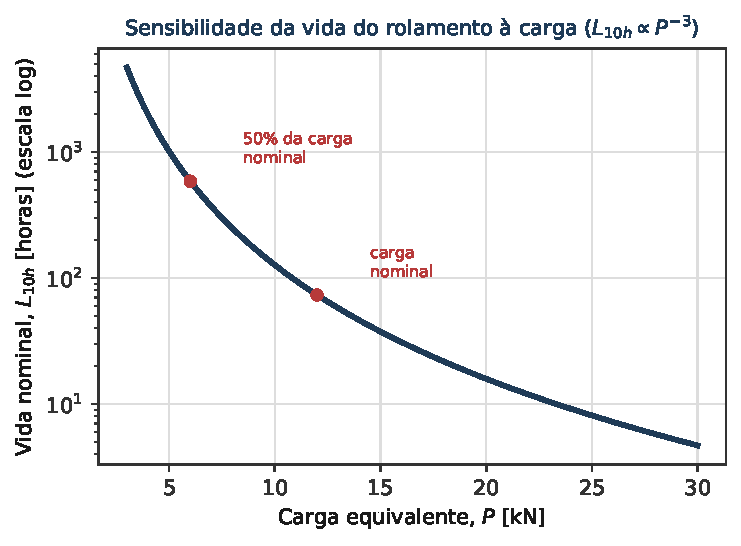
\includegraphics[width=0.60\textwidth]{figuras/fig_8_3_l10h.pdf}
			\caption[Sensibilidade da vida do rolamento à carga]{Sensibilidade da vida nominal do rolamento ($L_{10h}$) à carga equivalente — note a escala logarítmica no eixo vertical.}
			\label{fig:8-3}
		\end{figure}

		\item \textbf{Indicadores de Falha:} O modelo monitora frequências de pista externa (BPFO), interna (BPFI) e elementos rolantes (BSF), utilizando a \textit{Curtose} e o \textit{Fator de Crista} para identificar o início de \textit{spalling}.
	\end{itemize}

	\subsection{\textbf{Rotordinâmica e Velocidade Crítica}}
	A vida útil dos rolamentos (Equação~\eqref{eq:s8-4}) descreve o desgaste por fadiga de contato, mas não protege por si só contra o modo de falha mais súbito de eixos de alta rotação: a ressonância lateral. Os pinhões do estágio HP operam tipicamente acima da primeira velocidade crítica, exigindo que o Gêmeo Digital trate o eixo como um sistema rotordinâmico, não apenas como uma carga estática sobre o mancal.
	\begin{itemize}
		\item \textbf{Velocidade Crítica (Modelo de Jeffcott):} Aproximando o conjunto eixo-pinhão como um rotor de Jeffcott (massa concentrada $m$ sobre um eixo de rigidez lateral $k_s$, apoiado em mancais de rigidez $k_b$), a primeira velocidade crítica é dada pela Equação~\eqref{eq:s8-5}:
		\begin{equation}\label{eq:s8-5}
 \omega_{cr} = \sqrt{\frac{k_{eq}}{m}} \quad \text{onde} \quad \frac{1}{k_{eq}} = \frac{1}{k_s} + \frac{2}{k_b} 
\end{equation}
		A rigidez de mancal $k_b$ não é constante: em mancais hidrodinâmicos ela varia com a viscosidade $\mu(T)$ e a excentricidade, de modo que $\omega_{cr}$ se desloca com a temperatura de óleo e a carga — o Gêmeo Digital deve recalcular $\omega_{cr}$ em tempo real a partir de $T_{\text{oil}}$ e não tratá-la como constante de projeto.
		\item \textbf{Margem de Separação (API 684 \cite{api684}):} A norma exige margem mínima entre a velocidade de operação $\omega_{op}$ e qualquer velocidade crítica dentro da faixa de operação do VSD, formalizada na Equação~\eqref{eq:s8-6}:
		\begin{equation}\label{eq:s8-6}
 \left| \frac{\omega_{op} - \omega_{cr}}{\omega_{cr}} \right| \geq 0.20 \quad \text{(tipicamente } \pm 20\% \text{)} 
\end{equation}
		Como o VSD varre continuamente a faixa de rotação para casar a vazão com a demanda, o Gêmeo Digital deve verificar essa margem em cada ponto de operação comandado, e não apenas no projeto original — evitando que uma rampa de aceleração/desaceleração estacione o eixo em ressonância.
		\item \textbf{Diagnóstico via Diagrama de Campbell:} O cruzamento entre as linhas de excitação ($1\times$ RPM, $2\times$ RPM, frequência de engrenamento $GMF$) e as velocidades críticas identificadas por impacto ou \textit{run-up} é mapeado em um Diagrama de Campbell digital, atualizado com os dados de vibração em tempo real, permitindo detectar o deslocamento de $\omega_{cr}$ por desgaste de mancal antes que a margem de separação seja violada. A Figura~\ref{fig:8-2} exemplifica esse diagrama: as retas de excitação crescem linearmente com a rotação, a velocidade crítica é uma reta horizontal, e a faixa de operação do VSD (sombreada) deve evitar a zona de risco ao redor do cruzamento — exatamente o critério formalizado na Equação~\eqref{eq:s8-6}.
	\end{itemize}

	\begin{figure}[h!tbp]
		\centering
		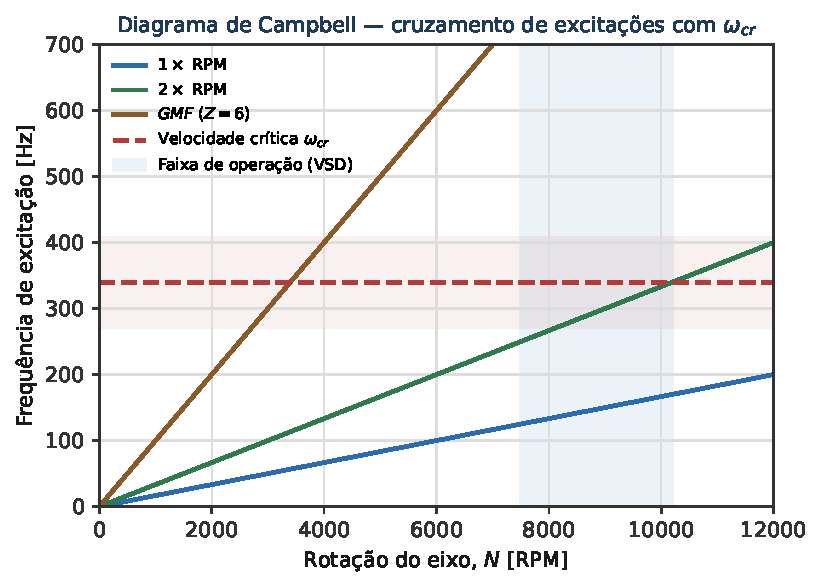
\includegraphics[width=0.75\textwidth]{figuras/fig_8_2_campbell.pdf}
		\caption[Diagrama de Campbell]{Diagrama de Campbell ilustrativo: cruzamento das linhas de excitação ($1\times$, $2\times$ RPM, GMF) com a velocidade crítica $\omega_{cr}$ e a faixa de operação do VSD.}
		\label{fig:8-2}
	\end{figure}

	\subsection{\textbf{Integridade dos Dentes e Modos de Falha de Engrenamento}}
	A saúde das engrenagens é avaliada através de modelos de fadiga de superfície e flexão.
	\begin{itemize}
		\item \textbf{Fadiga de Flexão (Tensão na Raiz - Lewis):} A Equação~\eqref{eq:s8-7} estima a tensão de flexão na base do dente da engrenagem — a força tangencial transmitida, dividida pela área efetiva da raiz do dente ($b \cdot m$) e pelo fator de forma de Lewis, e então ampliada por dois fatores de correção que penalizam efeitos dinâmicos ($K_v$) e distribuição desigual de carga ao longo da face ($K_m$):
		\begin{equation}\label{eq:s8-7}
 \sigma_b = \frac{W_t}{b \cdot m \cdot Y} \cdot K_v \cdot K_m
\end{equation}
		Onde $W_t$ é a força tangencial transmitida no dente, $b$ a largura de face da engrenagem, $m$ o módulo (geometria do dente), $Y$ é o fator de forma de Lewis, $K_v$ o fator dinâmico (velocidade de engrenamento) e $K_m$ o fator de distribuição de carga. A forma é a equação de flexão de Lewis, desenvolvida no capítulo de engrenagens cilíndricas e helicoidais de Shigley \cite[Cap.~14]{shigley}, com os fatores de correção na definição normalizada pela AGMA \cite{agma2001}. Uma trinca na raiz altera a rigidez, gerando impactos cíclicos no envelope de vibração.
		\item \textbf{Dano Adesivo (Scuffing):} O modelo calcula a Temperatura de Flash ($T_{\text{flash}}$) no contato instantâneo. Se $T_{\text{flash}} > T_{\text{crítica}}$, o sistema sinaliza falha iminente de lubrificação.
	\end{itemize}
	
	\subsection{\textbf{Desalinhamento e Arquiteturas de Acionamento}}
	\begin{itemize}
		\item \textbf{Desalinhamento:} Identificado por vibrações em $1 \times$ e $2 \times$ RPM (axial/radial). O desalinhamento interno eleva o fator $K_m$, concentrando tensões e reduzindo a vida útil das engrenagens.
		\item \textbf{Arquitetura Multi-Drive (Motores Independentes):} Elimina a \textit{gearbox} central, mas exige sincronismo eletrônico via VFD. A potência total é a soma individual, pela Equação~\eqref{eq:s8-8}:
		\begin{equation}\label{eq:s8-8}
 P_{\text{total}} = \sum \frac{\tau_i \cdot \omega_i}{\eta_{\text{mot},i}} 
\end{equation}
	\end{itemize}
	
	\subsection{\textbf{Matriz de Falhas de Transmissão}}
	A Tabela~\ref{tab:8-1} resume os principais modos de falha do trem de transmissão (rolamentos, dentes, sincronismo), suas causas raiz e o respectivo indicador digital de detecção.
	\begin{table}[h!tbp]
		\centering
		\small
		\renewcommand{\arraystretch}{1.5}
		\begin{tabular}{l l l}
			\toprule
			\textbf{Falha} & \textbf{Causa Raiz} & \textbf{Indicador Digital} \\ \midrule
			Desgaste de Rolamento & Fadiga / Contaminação & Picos em BPFO/BPFI e $\uparrow$ Curtose \\
			Pitting nos Dentes & Sobrecarga Cíclica & Bandas laterais na $GMF$ \\
			Quebra de Dente & Fadiga de Raiz (Lewis) & Impactos no envelope de vibração \\
			Desalinhamento & Montagem / Térmico & Vibração $2 \times \text{RPM}$ e $\uparrow K_m$ \\
			\textit{Scuffing} & Falha de Lubrificação & $\uparrow T$ de Flash e Partículas no Óleo \\
			Erro de Sincronismo & Desgaste \textit{Timing Gears} & Desvio de fase $\Delta \phi$ e oscilação de torque \\ \bottomrule
		\end{tabular}
		\caption[Matriz de falhas do trem de transmissão]{Matriz de falhas do trem de transmissão: rolamentos, dentes de engrenagem, alinhamento e sincronismo.}
		\label{tab:8-1}
	\end{table}
	
	\vspace{1em}
	\textbf{Condição de Estabilidade Mecânica:} A Equação~\eqref{eq:s8-9} resume, em duas desigualdades simultâneas, o critério de saúde de todo o trem de transmissão: a tensão real na raiz do dente (Equação~\eqref{eq:s8-7}) deve permanecer abaixo da tensão admissível do material, e o erro de fase entre os rotores de sincronismo deve permanecer menor que a folga de \textit{backlash} de projeto — a violação de qualquer uma indica risco iminente de quebra de dente ou contato metal-metal:
	\begin{equation}\label{eq:s8-9}
 \boxed{\sigma_{b, \text{real}} < \sigma_{b, \text{adm}} \quad \text{e} \quad \Delta \theta_{\text{sync}} < \theta_{\text{backlash}}}
\end{equation}

	\subsection{\textbf{Análise Torcional do Trem Completo}}
	A velocidade crítica $\omega_{cr}$ da Equação~\eqref{eq:s8-5} e a margem de separação da Equação~\eqref{eq:s8-6} tratam apenas do modo \textbf{lateral} de vibração do eixo — o rotor de Jeffcott flexiona transversalmente. Mas o conjunto motor–acoplamento–gearbox–rotores forma também um sistema massa-mola \textbf{torcional}, com seus próprios modos de ressonância em torção pura, independentes da rigidez lateral. Máquinas de alta potência exigem essa análise separadamente \cite{api684}: a rigidez torcional do eixo já calculada na Equação~\eqref{eq:s6-5} entra aqui como um dos elementos de um sistema de múltiplas inércias, não mais como um cálculo isolado de torção estática.

	Na aproximação de duas inércias — o rotor do motor ($I_1$) contra a inércia equivalente do trem de compressão referida ao eixo do motor ($I_2$, mesma referência já usada para $I_{\text{sys}}$ na Equação~\eqref{eq:s6-1}), conectadas pela rigidez torcional equivalente $k_{t,\text{eq}}$ (a associação em série da rigidez do eixo $k_t$ da Equação~\eqref{eq:s6-5} com a do acoplamento) — a frequência natural torcional fundamental é dada pela Equação~\eqref{eq:s8-10}:
	\begin{equation}\label{eq:s8-10}
 \omega_{cr,t} = \sqrt{k_{t,\text{eq}} \left( \frac{1}{I_1} + \frac{1}{I_2} \right)}
\end{equation}
	O critério de projeto exige a mesma lógica de margem de separação da Equação~\eqref{eq:s8-6}, mas contra um conjunto de excitações distinto: enquanto a ressonância lateral responde a $1\times$ RPM e $2\times$ RPM, a ressonância torcional é excitada também pela frequência de passagem de lóbulos ($f_{bp}$), pela frequência de engrenamento ($GMF$) e pelos harmônicos de torque gerados pelo chaveamento PWM do VSD (mesma origem física da distorção harmônica de corrente $\text{THD}_i$ já discutida no Capítulo de Subsistema Elétrico, agora manifestada como oscilação de torque em vez de corrente). Diferente da vibração lateral — que se manifesta como deslocamento radial detectável por acelerômetro — uma ressonância torcional pode não aparecer na carcaça: sua assinatura mais confiável é a oscilação cíclica do torque calculado, $\tau_{\text{ref}}$ da Equação~\eqref{eq:s6-8}, na frequência de $\omega_{cr,t}$.

	\vspace{1em}
	\hrule
	\vspace{1em}

	\textbf{Diretriz Técnica Final:} A Equação~\eqref{eq:s8-9} reúne as duas condições independentes de integridade do trem de transmissão — estrutural (fadiga do dente) e cinemática (sincronismo) — que devem ser satisfeitas simultaneamente; a violação de qualquer uma delas isoladamente já justifica a parada preventiva da máquina, mesmo que a outra permaneça dentro do limite. A Equação~\eqref{eq:s8-10} cobre um terceiro eixo de risco que nenhuma das duas anteriores captura: a ressonância torcional não quebra um dente nem desalinha o sincronismo diretamente, mas fadiga o próprio eixo e o acoplamento por ciclos de torque — e, ao contrário da vibração lateral já instrumentada no ponto B da Tabela~\ref{tab:18-1}, seu único sinal observável em campo costuma ser a oscilação do torque estimado, não uma leitura direta de sensor.

	% --- Fim do Capítulo 8 ---
	
	% --- Início do Capítulo 9: Termodinâmica do Estágio LP e Dinâmica de Folgas (Versão Integral) ---
	
	\clearpage
	\section{\textbf{Termodinâmica do Estágio LP, Dinâmica de Folgas e Resposta Vibracional}}
	\markboth{Termodinâmica do Estágio LP, Dinâmica de Folgas}{}

	Este capítulo detalha a física da compressão no primeiro estágio (LP), integrando a cinemática de engrenamento, o impacto das folgas micrométricas, o fenômeno de superaquecimento da carcaça e a assinatura vibracional resultante \cite{bently}. O modelo aqui descrito é a base para a detecção precoce de degradação nos rotores.
	
	\subsection{\textbf{Geometria de Engrenamento e Linha de Vedação}}
	O processo de compressão é definido pela variação volumétrica das câmaras formadas pela interação dos perfis dos rotores macho e fêmea.
	\begin{itemize}
		\item \textbf{Variação Volumétrica:} O volume $V$ é uma função do ângulo de rotação $\theta$. A taxa de variação temporal é dada pela Equação~\eqref{eq:s9-1}:
		\begin{equation}\label{eq:s9-1}
 \frac{dV}{dt} = \frac{dV}{d\theta} \cdot \omega 
\end{equation}
		\item \textbf{Área de Fuga Total ($A_{\text{leak}}$):} Representa a soma das passagens parasitas que permitem o retorno do gás entre câmaras de pressões distintas, pela Equação~\eqref{eq:s9-2}:
		\begin{equation}\label{eq:s9-2}
 A_{\text{leak}}(\theta) = L_{\text{seal}} \cdot \delta_f + L_{\text{tip}} \cdot \delta_r + A_{bh} 
\end{equation}
		Onde $L_{\text{seal}}$ é o comprimento da linha de vedação, $\delta_f$ a folga de flanco, $\delta_r$ a folga radial e $A_{bh}$ a área do triângulo de fuga (\textit{blow-hole}).
	\end{itemize}
	
	\subsection{\textbf{Dinâmica de Fugas e Razão de Pressão (\texorpdfstring{$\Pi$}{Pi})}}
	As folgas determinam a capacidade do estágio de sustentar a pressão e a eficiência volumétrica ($\eta_v$).
	\begin{itemize}
		\item \textbf{Eficiência Volumétrica e Folga:} O aumento da folga $\delta$ reduz a pressão efetiva de descarga $P_2$ para uma mesma rotação $\omega$, conforme a Equação~\eqref{eq:s9-3}:
		\begin{equation}\label{eq:s9-3}
 \eta_v = 1 - K \cdot \left( \frac{\delta}{L} \right) \cdot \sqrt{\frac{P_2}{P_1}} 
\end{equation}
		Onde $L$ é o comprimento de referência do rotor (normaliza a folga $\delta$) e $K$ é uma constante empírica de vazamento, calibrada por ensaio de desempenho da máquina (agrega efeitos de geometria do perfil e coeficiente de descarga não capturados explicitamente pelos demais termos). A Figura~\ref{fig:9-1} mostra que a queda de $\eta_v$ com o desgaste da folga é mais acentuada quanto maior a razão de pressão do estágio — ou seja, o mesmo desgaste físico penaliza proporcionalmente mais um estágio HP do que um estágio LP.

		\begin{figure}[h!tbp]
			\centering
			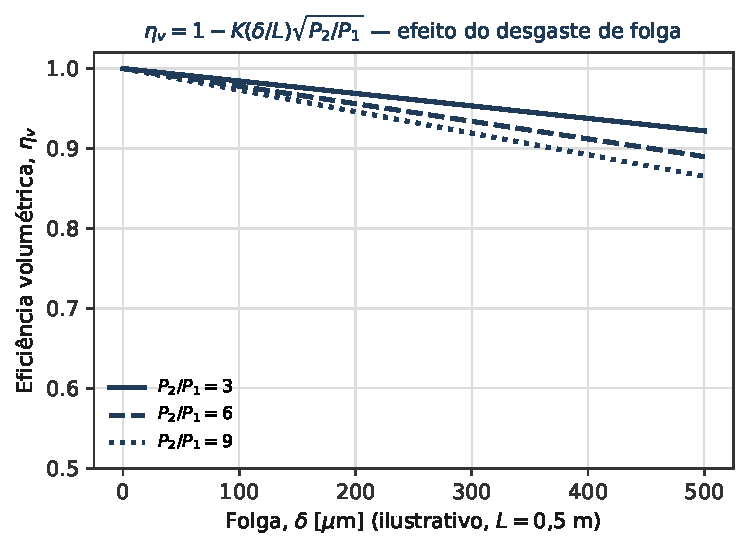
\includegraphics[width=0.60\textwidth]{figuras/fig_9_1_etav.pdf}
			\caption[Eficiência volumétrica em função da folga]{Eficiência volumétrica em função da folga do rotor, para diferentes razões de pressão do estágio.}
			\label{fig:9-1}
		\end{figure}
		\item \textbf{Fluxo de Massa de Fuga ($\dot{m}_{\text{leak}}$):} Modelado como escoamento compressível através de orifícios. O ar que retorna das câmaras de alta pressão reaquece o ar de sucção (\textit{pre-heating}), pela Equação~\eqref{eq:s9-4}:
		\begin{equation}\label{eq:s9-4}
 T_{\text{suc,eff}} = \frac{\dot{m}_{\text{in}} T_{\text{in}} + \dot{m}_{\text{leak}} T_{\text{leak}}}{\dot{m}_{\text{in}} + \dot{m}_{\text{leak}}} 
\end{equation}
		\item \textbf{Índice Politrópico ($n$):} O desvio da compressão adiabática ideal é monitorado pelo índice $n$, definido na Equação~\eqref{eq:s9-5}:
		\begin{equation}\label{eq:s9-5}
 n = \frac{\ln(P_2/P_1)}{\ln(P_2/P_1) - \ln(T_2/T_1)} 
\end{equation}
	\end{itemize}
	
	\subsection{\textbf{Superaquecimento da Carcaça e Dilatação Térmica}}
	A carcaça atua como dissipador térmico. O superaquecimento altera as folgas críticas por dilatação diferencial entre estator e rotor.
	\begin{itemize}
		\item \textbf{Balanço Térmico da Carcaça:} A Equação~\eqref{eq:s9-6} descreve como a temperatura da carcaça ($T_c$) evolui no tempo: sua capacidade térmica (massa $M_c$ vezes calor específico $c_c$) acumula a diferença entre o calor gerado internamente pela compressão ($\dot{Q}_{\text{int}}$) e o calor que consegue escapar — por convecção externa ($\dot{Q}_{\text{ext}}$) e pelo sistema de arrefecimento ($\dot{Q}_{\text{arref}}$):
		\begin{equation}\label{eq:s9-6}
 M_c c_c \frac{dT_c}{dt} = \dot{Q}_{\text{int}} - \dot{Q}_{\text{ext}} - \dot{Q}_{\text{arref}}
\end{equation}
		\item \textbf{Folga Residual Real ($\delta_{\text{real}}$):} O Gêmeo Digital calcula a folga instantânea considerando a expansão térmica dos rotores ($r$) e da carcaça ($c$), pela Equação~\eqref{eq:s9-7}:
		\begin{equation}\label{eq:s9-7}
 \delta_{\text{real}} = \delta_{\text{nom}} - (\alpha_r L_r \Delta T_r - \alpha_c L_c \Delta T_c) 
\end{equation}
		Se $\delta_{\text{real}} \to 0$, o modelo sinaliza risco iminente de contato (\textit{rubbing}).
	\end{itemize}
	
	\subsection{\textbf{Acoplamento Fluido-Estrutural e Resposta Vibracional}}
	A alteração nas folgas e na pressão interna gera forças de excitação mecânica detectáveis no espectro de frequência.
	\begin{itemize}
		\item \textbf{Frequência de Passagem dos Lóbulos ($f_{bp}$):} Assinatura principal do engrenamento — cada vez que um lóbulo do rotor macho passa por uma posição fixa da carcaça, ele gera um pulso de pressão. A Equação~\eqref{eq:s9-8} calcula a frequência desses pulsos multiplicando a frequência de giro do rotor macho pelo seu número de lóbulos ($Z_{\text{macho}}$). Como a rotação $N_{\text{macho}}$ é medida em RPM e $f_{bp}$ é expressa em Hz, é obrigatória a divisão por 60 — a mesma conversão já formalizada na Equação~\eqref{eq:s6-7}, e a fonte de erro mais comum ao configurar a faixa de análise espectral do sistema de monitoramento:
		\begin{equation}\label{eq:s9-8}
 f_{bp} = \frac{N_{\text{macho}}}{60} \cdot Z_{\text{macho}} = f_{r,\text{macho}} \cdot Z_{\text{macho}}
\end{equation}
		\item \textbf{Diagnóstico Vibracional:}
		\begin{itemize}
			\item \textbf{Aumento de Folgas:} Reduz o amortecimento pneumático entre rotores, elevando a amplitude em $f_{bp}$ e gerando pulsações de pressão na descarga.
			\item \textbf{Desalinhamento Térmico:} O gradiente de temperatura na carcaça causa empenamento (\textit{casing distortion}), resultando em picos em $1 \times$ e $2 \times$ RPM e aumento da vibração axial.
			\item \textbf{Contato (\textit{Rubbing}):} Caracterizado por emissões acústicas de alta frequência, picos não-harmônicos e aumento do ruído de fundo (\textit{noise floor}).
		\end{itemize}
	\end{itemize}
	
	\subsection{\textbf{Potência Real e Eficiência Isentrópica}}
	A potência absorvida pelo estágio LP ($\dot{W}_{\text{LP}}$) integra as perdas por fuga e calor. A eficiência isentrópica $\eta_{is}$ é o principal KPI de saúde, na Equação~\eqref{eq:s9-9}:
	\begin{equation}\label{eq:s9-9}
 \dot{W}_{\text{LP}} = \frac{\dot{m} \cdot c_p \cdot T_1}{\eta_{is}} \left[ \left( \frac{P_2}{P_1} \right)^{\frac{\gamma - 1}{\gamma}} - 1 \right] 
\end{equation}
	
	\subsection{\textbf{Matriz de Falhas Integrada do Estágio LP}}
	A Tabela~\ref{tab:9-1} integra os modos de falha do estágio LP com seus indicadores digitais e a assinatura vibracional correspondente, permitindo diferenciar causas puramente térmicas de causas mecânicas.
	\begin{table}[h!tbp]
		\centering
		\renewcommand{\arraystretch}{1.5}
		\resizebox{\textwidth}{!}{
		\begin{tabular}{l l l l}
			\toprule
			\textbf{Falha} & \textbf{Causa Raiz} & \textbf{Indicador Digital} & \textbf{Resposta Vibracional} \\ \midrule
			Desgaste de Folgas & Erosão / Particulados & $\downarrow \Pi$ e $\downarrow \eta_v$ & $\uparrow$ Amplitude em $f_{bp}$ \\
			Superaquecimento & Falha Arrefecimento & $\uparrow T_c$ e $\uparrow T_2$ & $\uparrow$ Vibração Axial \\
			Contato (\textit{Rubbing}) & Dilatação Térmica & $\uparrow \uparrow T_2$ súbito & Picos HF / Emissão Acústica \\
			Perda de \textit{Coating} & Ciclos Térmicos & $\uparrow n$ (Politrópico) & $\uparrow$ Ruído de fundo \\
			Erosão do Perfil & Contaminação & $\uparrow A_{\text{leak}}$ calculado & Bandas laterais em $f_{bp}$ \\
			Desalinhamento & Falha Sincronismo & Oscilação de Torque & Picos em $1 \times$ e $2 \times$ RPM \\ \bottomrule
		\end{tabular}
		}
		\caption[Matriz de falhas integrada do estágio LP]{Matriz de falhas integrada do estágio LP: causa raiz, indicador digital e assinatura vibracional.}
		\label{tab:9-1}
	\end{table}
	
	\vspace{1em}
	\textbf{Condição de Alerta de Saúde do Estágio:} A Equação~\eqref{eq:s9-10} consolida os quatro sintomas discutidos neste capítulo — desvio na razão de pressão ($\Delta\Pi$), queda na eficiência isentrópica ($\Delta\eta_{is}$), aumento de vibração ($\Delta\text{Vib}$) e redução da folga residual ($\delta_{\text{real}}$) — em uma única função de saúde do estágio LP:
	\begin{equation}\label{eq:s9-10}
 \boxed{Health\_Index = f(\Delta \Pi, \Delta \eta_{is}, \Delta \text{Vib}, \delta_{\text{real}})}
\end{equation}

	\subsection{\textbf{Relação entre Eficiência Politrópica e Isentrópica}}
	Este capítulo usa $\eta_{is}$ (Equação~\eqref{eq:s9-9}) como KPI de saúde do estágio, e o índice politrópico $n$ (mesmo índice da Equação~\eqref{eq:s5-5}) como parâmetro do processo real de compressão — mas nunca a relação entre os dois. A distinção importa porque folhas de dados de fabricante de máquinas de alta potência frequentemente especificam a eficiência \textbf{politrópica} ($\eta_p$), não a isentrópica, e sem a conversão o Gêmeo Digital não consegue confrontar o modelo diretamente contra a garantia contratual do equipamento. A eficiência politrópica é definida a partir do próprio índice $n$ e do $\gamma$ do ar \cite{moran, cengel, hanlon}, pela Equação~\eqref{eq:s9-11}:
	\begin{equation}\label{eq:s9-11}
 \eta_p = \frac{\gamma - 1}{\gamma} \cdot \frac{n}{n - 1}, \qquad
 \eta_{is} = \frac{\Pi^{(\gamma-1)/\gamma} - 1}{\Pi^{(\gamma-1)/(\gamma\,\eta_p)} - 1}
\end{equation}
	A diferença física entre as duas eficiências é o que torna a Equação~\eqref{eq:s9-11} necessária, e não apenas uma curiosidade algébrica: $\eta_p$ é uma propriedade essencialmente \textbf{local} do processo de compressão (praticamente constante ao longo do mapa de operação da máquina, pois depende só de $n$ e $\gamma$), enquanto $\eta_{is}$ compara o processo real contra um caminho isentrópico fixo entre a mesma sucção e a mesma descarga — e por isso varia com a razão de pressão $\Pi$ mesmo que a máquina não tenha degradado nada. As duas eficiências não são intercambiáveis: um $\eta_{is}$ que cai ao operar em $\Pi$ mais alto não é, por si só, evidência de degradação — pode ser simplesmente a assinatura esperada de $\eta_p$ constante sob razão de pressão maior. O Gêmeo Digital deve monitorar $\eta_p$ (via Equação~\eqref{eq:s9-11}, invertida a partir de $n$ medido) como o indicador limpo de degradação real do estágio, e reservar $\eta_{is}$ para comparação direta com a garantia de fábrica na condição de projeto.

	\subsection{\textbf{Velocidade Periférica e Número de Mach na Ponta do Rotor}}
	As Equações~\eqref{eq:s9-2} e~\eqref{eq:s9-3} tratam a fuga através das folgas em função da geometria estática ($A_{\text{leak}}$) e da razão de pressão, mas nunca amarram esse escoamento à rotação do rotor — o parâmetro que efetivamente determina o regime do escoamento de fuga pela folga é a velocidade da própria superfície por onde o gás escapa. A velocidade periférica da ponta do rotor macho é dada pela Equação~\eqref{eq:s9-12}:
	\begin{equation}\label{eq:s9-12}
 u_{\text{tip}} = \frac{\pi \cdot D_{\text{macho}} \cdot N_{\text{macho}}}{60}
\end{equation}
	Onde $N_{\text{macho}}$ é a mesma rotação (RPM) do rotor macho já usada na Equação~\eqref{eq:s9-8} para a frequência de passagem de lóbulos, e o fator $60$ cumpre a mesma função de conversão para segundos. Comparando $u_{\text{tip}}$ com a velocidade do som local $a = \sqrt{\gamma R T}$ obtém-se o número de Mach na ponta, pela Equação~\eqref{eq:s9-13}:
	\begin{equation}\label{eq:s9-13}
 M_{\text{tip}} = \frac{u_{\text{tip}}}{a}
\end{equation}
	O papel de $M_{\text{tip}}$ é duplo. No vazamento pela folga (Equações~\eqref{eq:s9-2}--\eqref{eq:s9-3}), ele indica se o escoamento de fuga se aproxima do regime compressível/sônico — condição em que a vazão de fuga deixa de crescer proporcionalmente com $\Delta P$ e satura, alterando a forma esperada da própria Equação~\eqref{eq:s9-3}. No projeto do rotor, $M_{\text{tip}}$ é o limite físico que a geometria assimétrica de perfil precisa respeitar para manter a operação isenta de óleo estável e silenciosa \cite{fleming, hanlon} — velocidades de ponta elevadas demais aumentam perdas aerodinâmicas e ruído independentemente de qualquer degradação, de modo que um $M_{\text{tip}}$ crescente ao longo do tempo para a mesma rotação nominal é, em si, um sintoma a investigar (deriva de $D_{\text{macho}}$ efetivo por desgaste, ou erro de calibração de $T$ na estimativa de $a$).

	\subsection{\textbf{Fechamento do Balanço Térmico da Carcaça}}
	A Equação~\eqref{eq:s9-6} descreve como $T_c$ evolui no tempo, mas nenhum de seus três termos ($\dot{Q}_{\text{int}}$, $\dot{Q}_{\text{ext}}$, $\dot{Q}_{\text{arref}}$) foi, até aqui, expresso em função de grandezas já medidas ou já calculadas pelo Gêmeo Digital — a mesma lacuna que a Equação~\eqref{eq:s10-7} fechou para $P_{\text{sat}}(T)$ no capítulo seguinte. Fechar essa lacuna é o que permite estimar $T_c$ (e, por extensão, avaliar o risco de contato da Equação~\eqref{eq:s9-7}) mesmo em plantas offshore sem instrumentação dedicada de temperatura de carcaça.

	O calor gerado internamente é dominado pela mesma perda mecânica já contabilizada no denominador $\eta_{\text{mec}}$ da Equação~\eqref{eq:s5-5} — atrito de rotores e mancais que não se converte em trabalho de compressão e permanece na máquina como calor, pela Equação~\eqref{eq:s9-14}:
	\begin{equation}\label{eq:s9-14}
 \dot{Q}_{\text{int}} = \dot{W}_{\text{LP}} \cdot (1 - \eta_{\text{mec}})
\end{equation}
	O calor que escapa da carcaça segue dois caminhos independentes, ambos regidos pela lei de Newton do resfriamento — proporcionais à diferença entre a temperatura da carcaça e a do ambiente ($T_c - T_{amb}$) — cada um com sua própria condutância térmica agregada: convecção natural pela superfície exposta da carcaça ($G_{\text{ext}}$) e o sistema de arrefecimento ativo do invólucro, tipicamente a ventilação forçada do \textit{hood} já descrita no Capítulo 2 ($G_{\text{arref}}$) — Equação~\eqref{eq:s9-15}:
	\begin{equation}\label{eq:s9-15}
 \dot{Q}_{\text{ext}} = G_{\text{ext}} \cdot (T_c - T_{amb}), \qquad
 \dot{Q}_{\text{arref}} = G_{\text{arref}} \cdot (T_c - T_{amb})
\end{equation}
	Substituindo as Equações~\eqref{eq:s9-14} e~\eqref{eq:s9-15} na Equação~\eqref{eq:s9-6} e resolvendo em regime permanente ($dT_c/dt=0$, a condição típica de operação estabilizada, sem evento transiente recente de carga), a temperatura de carcaça se torna uma função direta de grandezas já calculadas neste capítulo, pela Equação~\eqref{eq:s9-16}:
	\begin{equation}\label{eq:s9-16}
 T_{c} = T_{amb} + \frac{\dot{Q}_{\text{int}}}{G_{\text{ext}} + G_{\text{arref}}}
\end{equation}
	A rapidez com que a carcaça reage a uma mudança de carga (partida, alívio, evento de pico de demanda) é dada pela constante de tempo do sistema de primeira ordem definido pela linearização acima — razão entre a capacidade térmica da carcaça ($M_c$, $c_c$, já introduzidos na Equação~\eqref{eq:s9-6}) e a condutância total de dissipação — Equação~\eqref{eq:s9-17}:
	\begin{equation}\label{eq:s9-17}
 \tau_c = \frac{M_c \, c_c}{G_{\text{ext}} + G_{\text{arref}}}
\end{equation}
	Fora do regime permanente, a mesma linearização dá a solução transiente de primeira ordem $T_c(t) = T_{c} + (T_{c,0} - T_{c}) \cdot e^{-t/\tau_c}$, com $T_c$ da Equação~\eqref{eq:s9-16} e $T_{c,0}$ a condição inicial — a aproximação exponencial ao regime permanente após um degrau de $\dot{Q}_{\text{int}}$, forma idêntica à já usada para a resposta em rampa do inversor de frequência (Capítulo 13).

	Esse fechamento não substitui a Equação~\eqref{eq:s9-7}: mesmo com $T_c$ calculável, a folga residual $\delta_{\text{real}}$ segue dependendo da temperatura do próprio rotor ($T_r$), que este documento não modela por um balanço térmico equivalente — permanece, por ora, uma grandeza a ser medida ou estimada por um modelo à parte, fora do escopo fechado por esta seção.

	\textbf{Ressalva sobre $T_{amb}$ em instalações com invólucro:} as Equações~\eqref{eq:s9-15}--\eqref{eq:s9-17} usam $T_{amb}$ como referência de convecção da carcaça, o que só é fisicamente correto para um compressor a céu aberto. Quando o elemento compressor está confinado no mesmo invólucro acústico que o motor, o VSD e a gearbox — arranjo comum em pacotes offshore por restrição de ruído, cobrindo às vezes o trem inteiro até a saída do 2º estágio (Capítulo 2) —, o ar que efetivamente banha a carcaça não é o ambiente externo, e sim o ar interno do invólucro, já aquecido pelas demais fontes de calor confinadas. Nesse caso, $T_{amb}$ nas três equações acima deve ser lido como $T_{\text{hood}}$, fechado pela Equação~\eqref{eq:s2-4} do Capítulo 2 — não como reescrita das equações (a forma matemática é idêntica), mas como reinterpretação do termo de referência. A ordem de cálculo correta está detalhada naquela seção.

	\vspace{1em}
	\hrule
	\vspace{1em}

	\textbf{Diretriz Técnica Final:} O Índice de Saúde da Equação~\eqref{eq:s9-10} só é interpretável se cada uma de suas quatro entradas ($\Pi$, $\eta_{is}$, vibração, $\delta_{\text{real}}$) for rastreada individualmente na Matriz de Falhas apresentada acima — reduzir tudo a um único número sem manter o detalhamento por causa raiz transforma um diagnóstico acionável em apenas mais um alarme genérico. A Equação~\eqref{eq:s9-11} adiciona a mesma cautela ao próprio $\Delta\eta_{is}$ que alimenta esse índice: antes de contar uma queda de $\eta_{is}$ como sintoma de falha, o Gêmeo Digital deve descontar a parcela que é apenas o efeito esperado de operar em razão de pressão distinta do ponto de garantia — só o resíduo depois desse desconto é degradação real. As Equações~\eqref{eq:s9-14}--\eqref{eq:s9-17} fecham o último elo puramente conceitual do capítulo: com elas, $T_c$ deixa de ser uma grandeza que só um sensor de carcaça poderia fornecer e passa a ser calculável a partir do próprio ponto de operação — mas a Equação~\eqref{eq:s9-17} também é um lembrete de escala: $\tau_c$ tipicamente responde em minutos a dezenas de minutos, ordem de grandeza muito maior que a dinâmica de pressão da rede (Capítulo 13) — um alarme de superaquecimento de carcaça nunca deve ser dimensionado com a mesma constante de tempo usada para a resposta do VSD.

	% --- Fim do Capítulo 9 ---
	
	% --- Início do Capítulo 10: Intercooler, Condensado e Distúrbios de Rede ---
	
	\clearpage
	\section{\textbf{Dinâmica do Intercooler, Gestão de Condensado e Distúrbios de Rede}}
	
	Este capítulo detalha a modelagem do resfriamento intermediário, integrando a termodinâmica de troca térmica, a psicrometria de condensação e a distinção entre falhas internas e distúrbios operacionais externos, como o impacto térmico de operações de \textit{offloading}.
	
	\subsection{\textbf{Termodinâmica de Troca Térmica e Efetividade}}
	O intercooler opera como um trocador de calor de correntes cruzadas ou contracorrente. A taxa de transferência de calor ($\dot{Q}$) é governada pelo balanço de energia e pela equação de transferência global, na Equação~\eqref{eq:s10-1}:

	\begin{equation}\label{eq:s10-1}
	\begin{aligned}
		\dot{Q} &= \dot{m}_a \cdot c_{p,a} \cdot (T_{LP,\text{out}} - T_{HP,\text{in}}) \\[4pt]
		\dot{Q} &= U \cdot A \cdot \Delta T_{lm} \cdot F
	\end{aligned}
\end{equation}
	
	Onde $\Delta T_{lm}$ é a Diferença de Temperatura Média Logarítmica (LMTD), forma fechada clássica para a força motriz térmica em trocadores de calor \cite{cengel, incropera}, dada pela Equação~\eqref{eq:s10-2}:

	\begin{equation}\label{eq:s10-2}
	\Delta T_{lm} = \frac{(T_{LP,\text{out}} - T_{w,\text{out}}) - (T_{HP,\text{in}} - T_{w,\text{in}})}{\ln \left( \frac{T_{LP,\text{out}} - T_{w,\text{out}}}{T_{HP,\text{in}} - T_{w,\text{in}}} \right)}
\end{equation}

	A origem física dessa expressão logarítmica fica clara ao observar o perfil de temperatura ao longo do trocador (Figura~\ref{fig:10-1}): como a diferença de temperatura entre os dois fluidos ($\Delta T_1$ na entrada, $\Delta T_2$ na saída) varia continuamente ao longo do comprimento, a força motriz térmica ``média'' correta não é a média aritmética simples, e sim a média logarítmica dessas duas diferenças extremas.

	\begin{figure}[h!tbp]
		\centering
		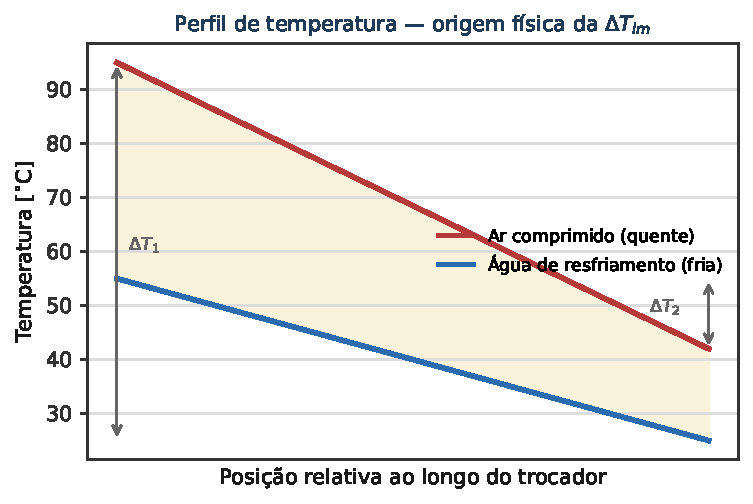
\includegraphics[width=0.60\textwidth]{figuras/fig_10_1_lmtd.pdf}
		\caption[Perfil de temperatura e origem física da LMTD]{Perfil de temperatura ao longo de um trocador em contracorrente — origem física da LMTD.}
		\label{fig:10-1}
	\end{figure}

	Para isolar a performance do ativo das flutuações da planta, o Gêmeo Digital monitora a Efetividade ($\epsilon$), pela Equação~\eqref{eq:s10-3}:

	\begin{equation}\label{eq:s10-3}
	\epsilon = \frac{T_{LP,\text{out}} - T_{HP,\text{in}}}{T_{LP,\text{out}} - T_{w,\text{in}}}
\end{equation}
	
	\subsection{\textbf{Mecanismo de Falha Externa: Sobrecarga Térmica (\textit{Offloading})}}
	Durante operações de \textit{offloading}, a temperatura da água de resfriamento ($T_{w,\text{in}}$) aumenta devido à demanda de outros consumidores. O Gêmeo Digital quantifica a penalidade de potência no estágio HP resultante deste distúrbio, pela Equação~\eqref{eq:s10-4}:

	\begin{equation}\label{eq:s10-4}
	\begin{aligned}
		\Delta \dot{W}_{\text{penalty}} &= \dot{W}_{HP}(T_{w,\text{in,atual}}) - \dot{W}_{HP}(T_{w,\text{in,nominal}}) \\[4pt]
		\dot{W}_{HP} &= \frac{\dot{m} \cdot R \cdot T_{HP,\text{in}}}{\eta_{is}} \cdot \left( \frac{n}{n-1} \right) \cdot \left[ \left( \frac{P_{HP,\text{out}}}{P_{HP,\text{in}}} \right)^{\frac{n-1}{n}} - 1 \right]
	\end{aligned}
\end{equation}
	
	\textbf{Diagnóstico:} Se $\epsilon$ permanece constante enquanto $T_{HP,\text{in}}$ e $\dot{W}_{HP}$ aumentam, o modelo classifica o evento como \textit{External Thermal Disturbance}.
	
	\subsection{\textbf{Mecanismo de Falha Interna: Incrustação (\textit{Fouling})}}
	A degradação interna é modelada pelo acúmulo de resistência térmica adicional ($R_f$). O coeficiente global de transferência real ($U_{\text{real}}$) é comparado ao valor de projeto ($U_{\text{clean}}$). A Equação~\eqref{eq:s10-5} nada mais é que a definição de resistência térmica global em série \cite[Cap.~11]{incropera}, escrita de modo que a incrustação apareça como uma resistência acrescentada ao caminho térmico limpo — e, na forma isolada à direita, como grandeza calculável a partir de medições de campo:
	
	\begin{equation}\label{eq:s10-5}
	\frac{1}{U_{\text{real}}} = \frac{1}{U_{\text{clean}}} + R_f \implies R_f = \frac{A \cdot \Delta T_{lm}}{\dot{Q}} - \frac{1}{U_{\text{clean}}}
\end{equation}
	
	O Gêmeo Digital utiliza a tendência de $R_f$ para prever a saturação térmica do trocador.
	
	\subsection{\textbf{Psicrometria e Extração de Condensado}}
	O resfriamento do ar comprimido frequentemente atinge o ponto de orvalho. A massa de água líquida gerada ($\dot{m}_{\text{cond}}$) é calculada pela variação da umidade específica ($W$ — convenção ASHRAE \cite{ashrae} para razão de umidade, evitando colisão com a velocidade angular $\omega$), pela Equação~\eqref{eq:s10-6}:

	\begin{equation}\label{eq:s10-6}
	\begin{aligned}
		W &= 0.622 \cdot \frac{\phi \cdot P_{\text{sat}}(T)}{P - \phi \cdot P_{\text{sat}}(T)} \\[4pt]
		\dot{m}_{\text{cond}} &= \dot{m}_a \cdot (W_{\text{in}} - W_{\text{out}})
	\end{aligned}
\end{equation}

	Até este ponto do documento, $P_{\text{sat}}(T)$ é referenciada como variável de processo, mas nunca definida como função constitutiva — o que impede o Gêmeo Digital de calculá-la a partir de $T$ medida. Para o intervalo de temperaturas típico do resfriamento de ar comprimido offshore ($0\,^{\circ}\text{C}$ a $80\,^{\circ}\text{C}$), a correlação de Arden Buck \cite{buck}, na Equação~\eqref{eq:s10-7}, oferece precisão adequada sem exigir tabelas de vapor:
	\begin{equation}\label{eq:s10-7}
 P_{\text{sat}}(T) = 0.61121 \, \exp\left[ \left( 18.678 - \frac{T}{234.5} \right) \left( \frac{T}{257.14 + T} \right) \right] \quad [\text{kPa}, \; T \text{ em } ^{\circ}\text{C}]
\end{equation}
	A Figura~\ref{fig:10-2} mostra essa correlação em escala logarítmica: a pressão de saturação praticamente dobra a cada 10-12$^{\circ}$C de aumento de temperatura, o que explica por que uma pequena falha de resfriamento no aftercooler tem efeito desproporcional na quantidade de água que chega ao secador PSA a jusante.

	\begin{figure}[h!tbp]
		\centering
		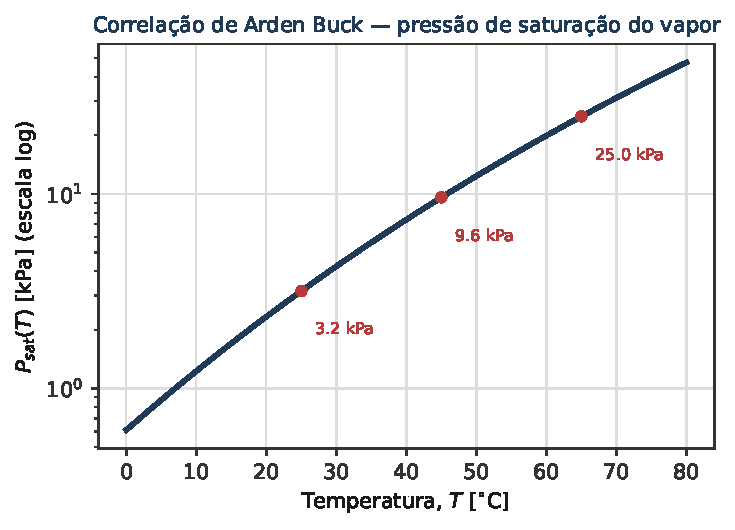
\includegraphics[width=0.60\textwidth]{figuras/fig_10_2_psat.pdf}
		\caption[Correlação de Arden Buck]{Correlação de Arden Buck para a pressão de saturação do vapor d'água em função da temperatura.}
		\label{fig:10-2}
	\end{figure}

	De forma análoga, o calor específico do ar úmido ($c_{p,\text{úmido}}$), usado implicitamente nas equações de $\dot{Q}$ e $\Delta T_{\text{oil}}$ ao longo deste capítulo, não é uma constante — ele deve incorporar a fração mássica de vapor d'água via $W$, pela Equação~\eqref{eq:s10-8}:
	\begin{equation}\label{eq:s10-8}
 c_{p,\text{úmido}} = c_{p,\text{ar seco}} + W \cdot c_{p,\text{vapor}} \approx 1005 + W \cdot 1860 \quad [\text{J}\,\text{kg}^{-1}\,\text{K}^{-1}] 
\end{equation}
	Ignorar essa correção introduz um viés sistemático nos balanços de energia dos trocadores em condições de alta umidade relativa offshore, justamente o cenário mais crítico para o dimensionamento do secador PSA a jusante.

	\textbf{Falha de Drenagem e Arraste:} A falha no sistema de purga resulta em acúmulo de líquido, identificado pelo aumento da perda de carga ($\Delta P_{\text{ar}}$) e pela assinatura vibracional de alta frequência no estágio HP — Equação~\eqref{eq:s10-9}:

	\begin{equation}\label{eq:s10-9}
	\Delta P_{\text{ar,real}} = f(\dot{m}_a, \rho) + \Delta P_{\text{obstrução}}
\end{equation}
	
	\subsection{\textbf{Matriz de Falhas Integrada do Sistema Intermediário}}

	A Tabela~\ref{tab:10-1} diferencia os distúrbios externos (\textit{offloading}, baixo fluxo de água) das falhas internas do próprio intercooler (\textit{fouling}, drenagem), cada um com sua variável de controle e ação recomendada.
	\begin{table}[h!tbp]
		\centering
		\renewcommand{\arraystretch}{1.5}
		\resizebox{\textwidth}{!}{
		\begin{tabular}{l l l l}
			\toprule
			\textbf{Mecanismo} & \textbf{Indicador Primário} & \textbf{Variável de Controle} & \textbf{Ação do Gêmeo} \\ \midrule
			\textit{Offloading} & $\uparrow T_{w,\text{in}}$ & $\epsilon \approx \text{constante}$ & Alerta de Rede Externa \\
			\textit{Fouling} & $\downarrow \epsilon$ e $\uparrow R_f$ & $U_{\text{real}} < U_{\text{limit}}$ & Sugestão de Limpeza \\
			Baixo Fluxo Água & $\uparrow \Delta T_{w}$ & $\downarrow \Delta P_{w}$ & Checar Bombas/Válvulas \\
			Falha Drenagem & $\uparrow \Delta P_{\text{ar}}$ & $\text{Vib}_{\text{HF,HP}} > \text{limit}$ & Alerta de Arraste/Erosão \\ \bottomrule
		\end{tabular}
		}
		\caption[Matriz de falhas do intercooler]{Matriz de falhas do intercooler: distúrbios externos versus falhas internas do trocador.}
		\label{tab:10-1}
	\end{table}
	
	\subsection{\textbf{Lógica de Predição de Trip e Saúde do Ativo}}
	O Índice de Saúde do Intercooler ($HI_{\text{IC}}$) e a predição de temperatura de descarga são calculados continuamente, pela Equação~\eqref{eq:s10-10}:

	\begin{equation}\label{eq:s10-10}
	\begin{cases}
		HI_{\text{IC}} = \omega_1 \cdot \left( \frac{\epsilon_{\text{real}}}{\epsilon_{\text{nom}}} \right) + \omega_2 \cdot \left( \frac{\Delta P_{\text{nom}}}{\Delta P_{\text{real}}} \right) \\[10pt]
		T_{HP,\text{out,pred}} = T_{HP,\text{in}} \cdot \Pi^{\frac{n-1}{n}}
	\end{cases}
\end{equation}
	
	Se $T_{HP,\text{out,pred}} \ge T_{\text{trip}}$, o Gêmeo Digital emite uma ordem de alívio de carga (\textit{load shedding}).

	\vspace{1em}
	\hrule
	\vspace{1em}

	\textbf{Diretriz Técnica Final:} A predição da Equação~\eqref{eq:s10-10} só tem valor preventivo se calculada com antecedência suficiente ao \textit{trip} — o Gêmeo Digital deve acionar o alívio de carga a partir da tendência projetada de $T_{HP,\text{out,pred}}$, não apenas quando o limite já tiver sido atingido pela medição real.

	% --- Fim do Capítulo 10 ---
	
	% --- Início do Capítulo 11: Estágio HP, Sincronismo e Integridade Mecânica ---
	
	\clearpage
	\section{\textbf{Estágio de Alta Pressão (HP), Sincronismo e Integridade Mecânica}}
	
	O estágio de Alta Pressão (HP) representa o maior desafio para o Gêmeo Digital, operando sob condições extremas de temperatura e pressão diferencial ($\Delta P$). Neste estágio, as folgas são reduzidas e qualquer desvio mecânico ou térmico pode resultar em falhas catastróficas.
	
	\subsection{\textbf{Termodinâmica e Performance do Estágio HP}}
	A compressão no estágio HP é modelada como um processo politrópico real, onde o índice $n$ reflete as perdas internas e a eficiência do resfriamento da carcaça. As duas equações que abrem esta seção não são correlações empíricas de fabricante: ambas descendem da expressão do trabalho de escoamento em processo internamente reversível, $w = \int v\,dP$, aplicada à relação politrópica $P v^{n} = \text{const.}$ — desenvolvimento clássico apresentado por Moran e colaboradores nos capítulos de entropia e de sistemas de potência a gás \cite[Cap.~6 e 9]{moran}.
	
	\begin{itemize}
		\item \textbf{Temperatura de Descarga Final ($T_{HP,\text{out}}$):} Aplicando a relação politrópica de temperatura-pressão à razão de compressão do estágio HP, a Equação~\eqref{eq:s11-1} projeta a temperatura de descarga a partir da temperatura de sucção e da razão entre as pressões de saída e entrada, elevada ao expoente politrópico:
		\begin{equation}\label{eq:s11-1}
 T_{HP,\text{out}} = T_{HP,\text{in}} \cdot \left( \frac{P_{HP,\text{out}}}{P_{HP,\text{in}}} \right)^{\frac{n-1}{n}}
\end{equation}
		
		\item \textbf{Potência Total Absorvida ($\dot{W}_{HP,\text{tot}}$):}
		A potência integra o trabalho termodinâmico e as perdas mecânicas nos rolamentos e engrenagens de sincronismo, pela Equação~\eqref{eq:s11-2}:
		\begin{equation}\label{eq:s11-2}
 \dot{W}_{HP,\text{tot}} = \frac{\dot{m} \cdot R \cdot T_{HP,\text{in}}}{\eta_{is}} \left( \frac{\gamma}{\gamma-1} \right) \left[ \left( \frac{P_{HP,\text{out}}}{P_{HP,\text{in}}} \right)^{\frac{\gamma-1}{\gamma}} - 1 \right] + \dot{W}_{\text{fric,rol}} + \dot{W}_{\text{eng}} 
\end{equation}
		
		\item \textbf{Eficiência Volumétrica ($\eta_{v,HP}$):}
		É extremamente sensível às folgas internas ($\delta$) e à pressão diferencial. A forma da Equação~\eqref{eq:s11-3} vem de tratar cada folga como um \textbf{orifício de descarga}: o produto $C_d \cdot A_{\text{gap}}(\delta) \cdot \sqrt{2 \rho \Delta P}$ é a vazão mássica de Bernoulli através de uma restrição de área $A_{\text{gap}}$, corrigida pelo coeficiente de descarga $C_d$, que absorve a contração da veia fluida e o desvio em relação ao escoamento ideal. É daí que vem uma consequência prática pouco intuitiva: a fuga cresce com a \textit{raiz} da pressão diferencial, não linearmente — dobrar $\Delta P$ aumenta o vazamento em cerca de $41\%$, não em $100\%$. O tratamento de referência para desempenho de compressores de deslocamento positivo, com seção dedicada aos de parafuso, está no \textit{Compressor Handbook} \cite[Cap.~1 e 2]{hanlon}:
		\begin{equation}\label{eq:s11-3}
 \eta_{v,HP} = 1 - \frac{\dot{m}_{\text{leak}}}{\dot{m}_{\text{th}}} = 1 - \frac{C_d \cdot A_{\text{gap}}(\delta) \cdot \sqrt{2 \rho \Delta P}}{\dot{m}_{\text{th}}} 
\end{equation}
	\end{itemize}
	
	\subsection{\textbf{Dinâmica de Sincronismo e Cargas Mecânicas}}
	As engrenagens de sincronismo (\textit{timing gears}) e os rolamentos garantem a operação isenta de óleo (\textit{oil-free}) mantendo os rotores sem contato.
	
	\begin{itemize}
		\item \textbf{Engrenagens de Sincronismo:}
		O erro de transmissão e o \textit{backlash} ($\theta_b$) são monitorados para evitar o contato entre os lobos. O \textit{backlash} é a folga angular deliberadamente deixada entre os flancos dos dentes para acomodar dilatação térmica e o filme de lubrificante; seu crescimento por desgaste é o que degrada o sincronismo. A Equação~\eqref{eq:s11-4} expressa a folga de flanco residual como função dessa folga angular e do desgaste acumulado, sobre a mesma base de projeto de engrenagens que fornece a tensão de Lewis da Equação~\eqref{eq:s8-7} \cite[Cap.~13 e 14]{shigley}:
		\begin{equation}\label{eq:s11-4}
 \delta_{\text{flanco}} = f(\theta_b, \text{desgaste}) 
\end{equation}
		
		\item \textbf{Cargas nos Rolamentos de Escora (\textit{Thrust Bearings}):}
		O estágio HP gera um empuxo axial ($F_a$) massivo que deve ser equilibrado para evitar a colisão do rotor com a placa de descarga, pela Equação~\eqref{eq:s11-5}:
		\begin{equation}\label{eq:s11-5}
 F_a = (P_{HP,\text{out}} - P_{HP,\text{in}}) \cdot A_{\text{rotor}}
\end{equation}
		A Equação~\eqref{eq:s11-5} é um modelo — o sensor que fecha a malha entre esse modelo e a realidade física do mancal de escora é a sonda de proximidade de \textbf{posição axial} ($\delta_{ax}$), instrumentação de proximidade cuja prática a própria API 619 \cite{api619} referencia para máquinas desta classe de potência. O motivo de instrumentar posição, e não apenas vibração, é temporal: o desgaste do rolamento de escora se manifesta primeiro como uma deriva lenta e progressiva de $\delta_{ax}$ (o rotor ``caminha'' axialmente à medida que as pistas desgastam), muito antes de qualquer excitação vibratória mensurável aparecer — por isso $\delta_{ax}$ funciona como indicador de condição precoce para o mesmo modo de falha que a Equação~\eqref{eq:s11-6} projeta em horas restantes de vida.

		\item \textbf{Vida Útil Remanescente ($L_{10h}$):} Mesma formulação da vida nominal de rolamento apresentada na Equação~\eqref{eq:s8-4}, agora aplicada à carga axial equivalente do estágio HP ($P_{eq}$) e à rotação do eixo do estágio HP ($N_{\text{rot,HP}}$) — a Equação~\eqref{eq:s11-6} projeta as horas restantes de operação do rolamento de escora antes da falha por fadiga:
		\begin{equation}\label{eq:s11-6}
 L_{10h} = \left( \frac{C}{P_{eq}} \right)^p \cdot \frac{10^6}{60 \cdot N_{\text{rot,HP}}}
\end{equation}
		A rotação entra aqui em RPM, como em toda a família de equações de vida de rolamento deste documento — o fator $60$ do denominador é justamente a conversão para horas, e substituí-la pela velocidade angular $\omega$ (rad\,s$^{-1}$) produziria um resultado sem significado dimensional.
	\end{itemize}
	
	\subsection{\textbf{Mecanismos de Falha Detalhados}}
	
	\begin{enumerate}
		\item \textbf{Dilatação Térmica Diferencial e \textit{Rubbing}:}
		O aumento de $T_{w,\text{in}}$ (\textit{offloading}) eleva $T_{HP,\text{in}}$. A expansão térmica do rotor excede a da carcaça. A folga residual é dada pela Equação~\eqref{eq:s11-7}:
		\begin{equation}\label{eq:s11-7}
 \delta_{\text{res}} = \delta_{\text{nom}} - \alpha \cdot L \cdot (T_{\text{rotor}} - T_{\text{carcaça}}) 
\end{equation}
		Se $\delta_{\text{res}} \le 0$, ocorre contato metálico, detectado por picos de vibração e queda súbita de $\eta_{is}$.
		
		\item \textbf{Desgaste de Engrenagens e Perda de Sincronismo:}
		Causado por fadiga ou falha de lubrificação. O sintoma é o aumento dos harmônicos da frequência de engrenamento — Equação~\eqref{eq:s11-8}, mesma definição cinemática já usada no Capítulo de Engenharia do Trem de Transmissão — e alteração na fase vibracional entre os eixos:
		\begin{equation}\label{eq:s11-8}
 f_{gmf} = Z \cdot f_{\text{rot}}
\end{equation}
		
		\item \textbf{Falha de Selagem e \textit{Blow-by}:}
		Degradação dos selos de labirinto ou anéis de carvão. O Gêmeo Digital monitora o aumento da pressão no cárter ($P_{\text{cárter}}$) e a redução da vazão mássica efetiva.
		
		\item \textbf{Calço Hidráulico por Arraste de Condensado:}
		Falha no dreno do intercooler. O líquido incompressível gera um pico de torque instantâneo ($\Delta \tau$), pela Equação~\eqref{eq:s11-9}:
		\begin{equation}\label{eq:s11-9}
 \Delta \tau = I \cdot \frac{d\omega}{dt} + \tau_{\text{impacto}}
\end{equation}
		Resulta em quebra de dentes de engrenagens ou cisalhamento de chavetas.
		
		\item \textbf{Degradação do Revestimento (\textit{Coating}):}
		Erosão ou alta temperatura causam o aumento progressivo do índice politrópico $n$ e do Consumo de Potência Específica ($SPC$).
	\end{enumerate}
	
	\subsection{\textbf{Matriz de Diagnóstico do Estágio HP}}

	A Tabela~\ref{tab:11-1} resume os cinco modos de falha críticos do estágio HP e seu impacto relativo no Consumo de Potência Específica (SPC), permitindo priorizar a resposta do Gêmeo Digital.
	\begin{table}[h!tbp]
		\centering
		\small
		\renewcommand{\arraystretch}{1.5}
		\begin{tabular}{l l l c}
			\toprule
			\textbf{Falha} & \textbf{Indicador Primário} & \textbf{Variável de Controle} & \textbf{Impacto SPC} \\ \midrule
			\textit{Rubbing} Térmico & $\uparrow$ Vibração Global & $T_{HP,\text{out}} > T_{\text{limit}}$ & $\uparrow \uparrow$ \\
			Desgaste \textit{Gears} & $\uparrow$ Harmônicos $f_{gmf}$ & Erro de Fase & $\uparrow$ \\
			Fadiga Rolamento & $\uparrow T_{\text{mancal}}$ & $L_{10h} \to 0$ & $\uparrow$ \\
			Vazamento Selos & $\uparrow P_{\text{cárter}}$ & $\downarrow \eta_{v,HP}$ & $\uparrow \uparrow$ \\
			Arraste Líquido & $\uparrow$ Emissão Acústica & Picos de Torque $\Delta \tau$ & Crítico \\ \bottomrule
		\end{tabular}
		\caption[Matriz de diagnóstico do estágio HP]{Matriz de diagnóstico do estágio HP e impacto relativo de cada falha no SPC.}
		\label{tab:11-1}
	\end{table}
	
	\subsection{\textbf{Indicador de Saúde Global e KPI Final}}
	O Gêmeo Digital consolida os desvios no Índice de Saúde ($HI_{HP}$), pela Equação~\eqref{eq:s11-10}:
	\begin{equation}\label{eq:s11-10}
 HI_{HP} = w_1 \left( \frac{\eta_{v,\text{real}}}{\eta_{v,\text{nom}}} \right) + w_2 \left( \frac{T_{\text{out,nom}}}{T_{\text{out,real}}} \right) + w_3 \left( \frac{V_{\text{nom}}}{V_{\text{real}}} \right) 
\end{equation}
	
	O Consumo de Potência Específica ($SPC$) é o KPI final, na Equação~\eqref{eq:s11-11}:
	\begin{equation}\label{eq:s11-11}
 \boxed{SPC = \frac{\dot{W}_{LP,\text{tot}} + \dot{W}_{HP,\text{tot}}}{\dot{V}_{\text{free\_air}}}} 
\end{equation}
	Unidade: $\text{kW} \cdotp \text{m}^{-3} \cdotp \text{min}$.

	O denominador da Equação~\eqref{eq:s11-11}, $\dot{V}_{\text{free\_air}}$, não é a vazão volumétrica lida em qualquer condição de linha — é a vazão mássica medida $\dot{m}$, convertida às condições de referência de admissão padronizadas pela ISO 1217:2009/Amd 1:2016 \cite{iso1217} (a mesma norma já citada no Capítulo 1 para $\eta_{is}$): pressão absoluta $P_{\text{ref}} = 1\,\text{bar}$, temperatura $T_{\text{ref}} = 20\,^{\circ}\text{C}$ e umidade relativa nula. A Equação~\eqref{eq:s11-12} formaliza essa conversão:
	\begin{equation}\label{eq:s11-12}
 \dot{V}_{\text{free\_air}} = \frac{\dot{m}}{\rho_{\text{ref}}}, \qquad \rho_{\text{ref}} = \frac{P_{\text{ref}}}{R \cdot T_{\text{ref}}}
\end{equation}
	É essa normalização — não a vazão bruta de um instrumento de campo qualquer — que torna o $SPC$ comparável entre um dia quente e um frio, entre plataformas com pressão atmosférica local distinta, e contra a folha de dados do fabricante, que reporta o FAD nominal exatamente nessas mesmas condições de referência.

	\vspace{1em}
	\hrule
	\vspace{1em}

	\textbf{Diretriz Técnica Final:} O SPC da Equação~\eqref{eq:s11-11} é o KPI comercial que a operação enxerga, mas sua causa raiz — quando se degrada — está quase sempre em um dos termos do Índice de Saúde da Equação~\eqref{eq:s11-10}; o Gêmeo Digital deve sempre apresentar os dois juntos, nunca o SPC isolado sem a decomposição por componente.

	% --- Fim do Capítulo 11 ---
	
	% --- Início do Capítulo 12: Sistema de Lubrificação e Gestão Térmica ---
	
	\clearpage
	\section{\textbf{Sistema de Lubrificação e Gestão Térmica}}

	Este capítulo revisita o circuito de óleo já introduzido no Capítulo de Trem de Potência e detalhado no Capítulo de Sistema de Lubrificação, agora sob a ótica específica da gestão térmica do conjunto gearbox/mancais em condições de carga do estágio HP. Como o compressor deste documento é isento de óleo na câmara de compressão (nenhum óleo entra em contato com o ar de processo — ver Capítulo de Arquitetura), o papel do óleo aqui é exclusivamente remover o calor gerado por atrito na caixa multiplicadora e nos mancais e devolvê-lo já resfriado ao circuito; o Gêmeo Digital monitora esse balanço térmico e a integridade do elemento deaerador em tempo real.

	\subsection{\textbf{Balanço de Energia do Circuito de Óleo}}
	A taxa de calor que o óleo remove do conjunto gearbox/mancais ($\dot{Q}_{\text{óleo}}$) é a mesma potência de atrito dissipada nesses componentes (Equações~\eqref{eq:s6-3}, \eqref{eq:s6-4} e \eqref{eq:s7-4}) — é fundamental mantê-la dentro da capacidade do resfriador para não elevar a temperatura de operação dos mancais além do limite do lubrificante — Equação~\eqref{eq:s12-1}:
	\begin{equation}\label{eq:s12-1}
 \dot{Q}_{\text{óleo}} = \dot{m}_{\text{óleo}} \cdotp c_{p,\text{óleo}} \cdotp (T_{\text{óleo,ret}} - T_{\text{óleo,sup}})
\end{equation}
	Onde $\dot{m}_{\text{óleo}}$ é a vazão mássica de óleo, $T_{\text{óleo,ret}}$ é a temperatura de retorno do óleo (já aquecido, saindo da gearbox/mancais) e $T_{\text{óleo,sup}}$ é a temperatura de suprimento após passar pelo resfriador de óleo — a mesma elevação de temperatura já modelada pelo balanço térmico do Capítulo de Sistema de Lubrificação (Equação~\eqref{eq:s7-5}), aqui reorganizada para isolar $\dot{Q}_{\text{óleo}}$ como a grandeza monitorada.

	\subsection{\textbf{Perda de Carga no Deaerador e Pressão de Suprimento aos Mancais}}
	Antes de alimentar os mancais e o engrenamento, o óleo de retorno passa por um separador de ar (deaerador) que libera as bolhas de ar incorporadas por respingo/turbulência durante a lubrificação — óleo aerado não sustenta o filme lubrificante nem dissipa calor com a mesma eficácia (ver Capítulo de Detalhamento de Componentes). A perda de carga nesse elemento ($\Delta P_{\text{sep}}$) cresce com a saturação e o tempo de uso; o modelo prevê a pressão que efetivamente chega aos mancais subtraindo essa perda da pressão de descarga da bomba de óleo ($P_{\text{bomba}}$, mantida pela bomba através da pressão $\Delta P_{\text{óleo}}$ já introduzida na Equação~\eqref{eq:s5-3}), pela Equação~\eqref{eq:s12-2}:
	\begin{equation}\label{eq:s12-2}
 P_{\text{sup,óleo}} = P_{\text{bomba}} - \Delta P_{\text{sep}}
\end{equation}
	Onde $\Delta P_{\text{sep}}$ é modelado em função da vazão volumétrica e da viscosidade cinemática do óleo $\nu(T)$. Uma queda de $P_{\text{sup,óleo}}$ abaixo do mínimo de projeto arrisca lubrificação insuficiente do engrenamento e dos mancais, mesmo que a vazão de óleo na saída da bomba esteja nominal.

	\subsection{\textbf{Capacidade do Resfriador: por que a Efetividade Não Basta}}
	O Capítulo 7 introduziu a efetividade $\epsilon$ (Equação~\eqref{eq:s7-6}) como indicador de saúde do resfriador de óleo, e ela cumpre bem esse papel enquanto as condições de contorno permanecem estáveis. Sob a carga do estágio HP em uma unidade offshore, porém, elas não permanecem estáveis: a temperatura de entrada da água de resfriamento acompanha a temperatura do mar e a carga dos demais consumidores do circuito de água, e a vazão disponível varia com a abertura de válvulas compartilhadas com outros equipamentos da planta. O problema é que $\epsilon$ responde a essas variações externas exatamente como responderia a uma incrustação interna — cai nos dois casos. Um alarme baseado apenas em $\epsilon$ é, portanto, ambíguo: ele não distingue ``o trocador sujou'' de ``a água de resfriamento chegou mais quente ou mais devagar''.

	A saída é monitorar a grandeza que descreve o trocador \textbf{independentemente} das temperaturas de entrada: a condutância térmica global $UA$ (produto do coeficiente global de transferência pela área de troca). Ela é obtida diretamente do calor efetivamente removido — já conhecido pela Equação~\eqref{eq:s12-1} — dividido pela diferença de temperatura média logarítmica entre óleo e água, pela Equação~\eqref{eq:s12-3}:
	\begin{equation}\label{eq:s12-3}
	UA_{\text{real}} = \frac{\dot{Q}_{\text{óleo}}}{\Delta T_{lm}}
	\end{equation}
	Onde $\Delta T_{lm}$ é a mesma LMTD já definida no Capítulo 10 para o intercooler, aqui aplicada ao par óleo/água. O ponto prático é que a Equação~\eqref{eq:s12-3} não exige instrumentação nova: as quatro temperaturas (entrada e saída de óleo, entrada e saída de água) e a vazão de óleo já são necessárias para o balanço da Equação~\eqref{eq:s12-1}.

	A relação entre as duas grandezas passa pelo número de unidades de transferência $NTU$ e pela razão de capacidades térmicas $C_r$, onde $C = \dot{m} \cdot c_p$ é a capacidade térmica de cada corrente. Para um trocador em contracorrente, a efetividade é uma função fechada dessas duas quantidades \cite{incropera}, conforme a Equação~\eqref{eq:s12-4}:
	\begin{equation}\label{eq:s12-4}
	\epsilon = \frac{1 - \exp\left[-NTU\,(1 - C_r)\right]}{1 - C_r \cdot \exp\left[-NTU\,(1 - C_r)\right]}, \qquad NTU = \frac{UA}{C_{\min}}, \qquad C_r = \frac{C_{\min}}{C_{\max}}
	\end{equation}
	A leitura diagnóstica da Equação~\eqref{eq:s12-4} é o que interessa ao Gêmeo Digital. A efetividade depende de $UA$, mas também de $C_{\min}$ — ou seja, das vazões. Uma redução na vazão de água de resfriamento derruba $\epsilon$ sem alterar em nada o estado físico do trocador. Já $UA$ só cai quando a superfície de troca de fato degrada: incrustação nos tubos, bolsão de ar retido no casco, tubos obstruídos ou vazamento interno. Normalizando pelo valor de projeto obtém-se um indicador adimensional de degradação, análogo à resistência de incrustação $R_f$ usada para o intercooler na Equação~\eqref{eq:s10-5}, mas expresso como fração da capacidade original — Equação~\eqref{eq:s12-5}:
	\begin{equation}\label{eq:s12-5}
	\eta_{UA} = \frac{UA_{\text{real}}}{UA_{\text{projeto}}}
	\end{equation}
	Um $\eta_{UA}$ estável com $\epsilon$ em queda aponta para fora da máquina — utilidade de água de resfriamento. Um $\eta_{UA}$ em queda sustentada aponta para dentro do trocador, e é ele, não $\epsilon$, que deve disparar a ordem de limpeza.

	\subsection{\textbf{Válvula Termostática e Temperatura de Suprimento}}
	A lógica da válvula termostática de três vias foi descrita qualitativamente no Capítulo 7; aqui ela é modelada, porque a mesma temperatura de suprimento pode resultar de posições de válvula muito diferentes, e essa distinção é diagnóstica. A válvula divide o óleo de retorno em dois ramos — um que atravessa o resfriador e outro que o desvia (\textit{bypass}) — e recombina os dois antes do suprimento aos mancais. Sendo $a_{tv}$ a fração da vazão enviada ao resfriador ($a_{tv}=1$: todo o óleo é resfriado; $a_{tv}=0$: todo o óleo desvia), a mistura resultante obedece à Equação~\eqref{eq:s12-6}:
	\begin{equation}\label{eq:s12-6}
	T_{\text{óleo,sup}} = a_{tv} \cdot T_{\text{óleo,fria}} + (1 - a_{tv}) \cdot T_{\text{óleo,ret}}
	\end{equation}
	Onde $T_{\text{óleo,fria}}$ é a temperatura na saída do resfriador e $T_{\text{óleo,ret}}$ a do óleo quente que retorna da gearbox. Como as três temperaturas são medidas, a equação pode ser invertida para \textbf{inferir} a posição efetiva da válvula, e o resíduo entre essa posição inferida e a posição comandada pelo controlador é o indicador direto de válvula travada — uma informação que a temperatura de suprimento sozinha não fornece, já que uma válvula presa pode, por coincidência de carga, entregar momentaneamente a temperatura correta.

	As duas formas de travamento têm consequências opostas e igualmente indesejáveis. Presa no \textit{bypass}, a válvula deixa o óleo aquecer sem controle, e a viscosidade despenca pela curva de Vogel da Equação~\eqref{eq:s7-2}, afinando o filme lubrificante dos mancais. Presa no resfriador, ela mantém o óleo frio demais na partida: a viscosidade excessiva eleva a potência de atrito da Equação~\eqref{eq:s7-4} e retarda o estabelecimento do filme hidrodinâmico justamente no momento de maior risco de contato metal-metal. O Gêmeo Digital trata os dois casos como falhas distintas, não como um alarme genérico de temperatura.

	\subsection{\textbf{Inércia Térmica e Tempo de Resposta do Circuito}}
	O circuito de óleo não responde instantaneamente. A massa de óleo em circulação armazena calor, e a temperatura de suprimento persegue o equilíbrio entre o calor gerado por atrito e o calor rejeitado pelo resfriador segundo o balanço transiente da Equação~\eqref{eq:s12-7}, cuja constante de tempo $\tau_{th}$ é a razão entre a capacidade térmica armazenada e a condutância do resfriador:
	\begin{equation}\label{eq:s12-7}
	M_{\text{óleo}} \cdot c_{p,\text{óleo}} \cdot \frac{dT_{\text{óleo,sup}}}{dt} = \dot{Q}_{\text{óleo}} - UA_{\text{real}} \cdot \Delta T_{lm}, \qquad \tau_{th} = \frac{M_{\text{óleo}} \cdot c_{p,\text{óleo}}}{UA_{\text{real}}}
	\end{equation}
	Onde $M_{\text{óleo}}$ é a massa de óleo do circuito (reservatório mais tubulação). O subscrito em $\tau_{th}$ evita colisão com o torque $\tau$ dos capítulos de transmissão, seguindo a convenção de desambiguação já adotada no documento.

	Essa constante de tempo tem duas consequências operacionais diretas. A primeira é de sintonia de alarme: após uma mudança de carga, a temperatura de óleo leva da ordem de $3\tau_{th}$ para acomodar no novo patamar, e um limiar de temperatura sem atraso mínimo dessa ordem transforma toda transição de carga em alarme falso. A segunda é diagnóstica e menos óbvia: $\tau_{th}$ é proporcional à massa de óleo do circuito. Se a resposta térmica observada fica sistematicamente \textbf{mais rápida} que a prevista, com $UA_{\text{real}}$ inalterado, a explicação física é que $M_{\text{óleo}}$ diminuiu — perda de carga de óleo por vazamento ou consumo. Esse é justamente o cenário ``Baixo Nível de Óleo'' da matriz a seguir, que por sintomas de regime permanente é ambíguo, mas pelo transiente é inequívoco.

	\subsection{\textbf{Mecanismos de Falha Térmica}}
	\begin{itemize}
		\item \textbf{Obstrução do Trocador de Calor:} Detectada pela queda sustentada de $\eta_{UA}$ (Equação~\eqref{eq:s12-5}), e não pela simples elevação da temperatura de suprimento — o resfriador deixou de rejeitar o calor esperado para a mesma carga térmica, com as condições de água inalteradas.
		\item \textbf{Degradação do Óleo:} Monitorada via desvio na condutividade térmica e aumento da temperatura de retorno do óleo para a mesma potência de atrito dissipada. Manifesta-se também como deriva dos coeficientes da curva de Vogel (Equação~\eqref{eq:s7-2}) ajustada aos dados de operação, já que o óleo oxidado não segue mais a curva $\mu \times T$ do lubrificante novo.
		\item \textbf{Travamento da Válvula Termostática:} Isolada pelo resíduo entre a posição $a_{tv}$ inferida da Equação~\eqref{eq:s12-6} e a posição comandada, com as duas direções de travamento produzindo falhas de natureza diferente (óleo quente demais em regime, ou frio e viscoso demais na partida).
		\item \textbf{Perda de Carga de Óleo:} Revelada pela redução da constante de tempo térmica $\tau_{th}$ (Equação~\eqref{eq:s12-7}) sem queda correspondente em $UA_{\text{real}}$ — um circuito com menos óleo aquece e esfria mais rápido do que o modelo prevê.
	\end{itemize}

	\subsection{\textbf{Matriz de Diagnóstico Térmico}}
	A Tabela~\ref{tab:12-1} cruza os sintomas de temperatura do óleo e perda de carga no deaerador para distinguir entre quatro causas raiz distintas de degradação térmica. A quarta coluna traz a grandeza modelada neste capítulo que confirma cada hipótese: as duas primeiras colunas levantam a suspeita, mas são as três últimas subseções que fecham o diagnóstico.
	\begin{table}[H]
		\centering
		\resizebox{\textwidth}{!}{
			\begin{tabular}{l c c c l}
				\toprule
				\textbf{Falha} & \textbf{Sintoma $T_{\text{óleo,ret}}$} & \textbf{Sintoma $\Delta P_{\text{sep}}$} & \textbf{Confirmação Quantitativa} & \textbf{Diagnóstico Digital} \\ \midrule
				Trocador Obstruído & $\uparrow \uparrow$ & Nominal & $\eta_{UA} \downarrow$ sustentado & \textbf{Falha no Arrefecimento} \\
				Deaerador Saturado & Nominal & $\uparrow \uparrow$ & $\eta_{UA}$ nominal & \textbf{Troca de Elemento Filtrante} \\
				Baixo Nível de Óleo & $\uparrow$ (Instável) & $\downarrow$ & $\tau_{th} \downarrow$ com $UA_{\text{real}}$ nominal & \textbf{Risco de Cavitação / Desgaste} \\
				Válvula Termostática Presa & $\uparrow$ ou $\downarrow$ & Nominal & Resíduo de $a_{tv}$ não nulo & \textbf{Falha de Controle Térmico} \\ \bottomrule
			\end{tabular}
		}
		\caption[Matriz de diagnóstico térmico do circuito de óleo]{Matriz de diagnóstico térmico do sistema de lubrificação e resfriamento, com a grandeza que confirma cada causa raiz.}
		\label{tab:12-1}
	\end{table}

	\subsection{\textbf{Balanço do Lado da Água: Soft-Sensor de Vazão}}
	A Equação~\eqref{eq:s12-4} calcula a efetividade $\epsilon$ a partir de $C_{\min}$, que depende da vazão de \textbf{ambos} os lados do trocador — mas o lado do óleo é sempre conhecido (o mesmo $\dot{m}_{\text{óleo}}$ da Equação~\eqref{eq:s12-1}) enquanto a vazão de água de resfriamento ($\dot{m}_w$) frequentemente não tem medidor dedicado em campo, por ser um utilidade compartilhada entre vários consumidores da planta. Sem $\dot{m}_w$ medido, não é possível determinar sequer qual dos dois lados é $C_{\min}$ na Equação~\eqref{eq:s12-4} — a mesma lacuna de observabilidade discutida na Diretriz Técnica Final do Capítulo 18 para outras grandezas.

	A saída, coerente com a filosofia de variáveis reais/virtuais já estabelecida na matriz do Capítulo 18, é tratar $\dot{m}_w$ como um \textbf{soft-sensor}: como $\dot{Q}_{\text{óleo}}$ já é conhecido pelo lado do óleo (Equação~\eqref{eq:s12-1}), e as duas temperaturas de água (entrada e saída do resfriador) são de instrumentação barata e comum, o próprio balanço de energia do lado da água pode ser invertido para inferir a vazão, pela Equação~\eqref{eq:s12-8}:
	\begin{equation}\label{eq:s12-8}
 \dot{m}_w = \frac{\dot{Q}_{\text{óleo}}}{c_{p,w} \cdot (T_{w,\text{out}} - T_{w,\text{in}})}
\end{equation}
	Esse $\dot{m}_w$ inferido não é redundante com um eventual medidor físico — é o substituto dele quando ele não existe, fechando a Equação~\eqref{eq:s12-4} e permitindo calcular $\eta_{UA}$ e distinguir incrustação interna de degradação da utilidade de água mesmo em pacotes sem instrumentação de vazão de água dedicada.

	\vspace{1em}
	\hrule
	\vspace{1em}

	\textbf{Diretriz Técnica Final:} A distinção entre os quatro cenários da matriz acima depende de observar $T_{\text{óleo,ret}}$ e $\Delta P_{\text{sep}}$ \textbf{simultaneamente} — isoladamente, cada sintoma é compatível com mais de uma causa raiz, e é justamente o cruzamento das variáveis que o Gêmeo Digital usa para eliminar a ambiguidade diagnóstica. O princípio que organiza este capítulo é mais geral e vale para qualquer subsistema térmico do compressor: sempre que um indicador de desempenho depender simultaneamente do equipamento e de suas condições de contorno — como $\epsilon$ depende de $UA$ e das vazões — ele serve para \textbf{detectar} o desvio, mas nunca para \textbf{atribuir} a causa. A atribuição exige uma grandeza invariante às condições externas ($UA$ para a superfície de troca, $a_{tv}$ para o atuador, $\tau_{th}$ para o inventário de óleo), e é por isso que o modelo do Gêmeo Digital precisa carregar a física do trocador, e não apenas seus limiares de alarme.

	% --- Início do Capítulo 13: Sistema de Controle, Válvulas e Estratégias de Modulação ---
	
	\clearpage
	\section{\textbf{Sistema de Controle, Válvulas e Estratégias de Modulação}}
	
	Este capítulo descreve a inteligência operacional do compressor, modelando a resposta dinâmica das válvulas e a lógica de controle para otimizar o consumo energético, operando com ou sem instrumentação de vazão.
	
	\subsection{\textbf{Dinâmica da Válvula de Admissão (\textit{Intake Valve})}}
	A válvula de admissão é o elemento que decide quanto ar entra na máquina, e por isso é o atuador primário de qualquer estratégia de modulação. Fisicamente ela se comporta como um orifício de área variável, comandado pelo solenoide de carga: o ar atmosférico é acelerado ao atravessar a restrição, e a vazão mássica resultante ($\dot{m}_{\text{in}}$) depende da área efetiva aberta, das condições do ar a montante e — de forma não linear — da razão entre a pressão a jusante e a pressão atmosférica. A Equação~\eqref{eq:s13-1} organiza esses três grupos de fatores, separando o que é geometria ($C_d \cdot A_v$), o que é estado do ar admitido ($P_{\text{atm}}$, $T_{\text{atm}}$) e o que é efeito de compressibilidade (a função de escoamento $\Phi(r)$):
	\begin{equation}\label{eq:s13-1}
 \dot{m}_{\text{in}} = C_d \cdotp A_v \cdotp P_{\text{atm}} \cdotp \sqrt{\frac{2}{R \cdotp T_{\text{atm}}}} \cdotp \Phi(r)
\end{equation}
	Onde $C_d$ é o coeficiente de descarga do orifício (perdas reais em relação ao escoamento isentrópico ideal, tipicamente obtido do ensaio da própria válvula), $A_v$ é a área efetiva de passagem comandada pelo atuador e $r = P_{\text{suc}}/P_{\text{atm}}$ é a razão de pressões através da válvula.

	A função $\Phi(r)$ merece atenção porque é onde reside o comportamento que distingue esse escoamento de um simples orifício hidráulico. Enquanto a pressão a jusante não cai muito, o escoamento é subsônico e a vazão cresce à medida que a diferença de pressão aumenta. A partir de certo ponto, porém, a velocidade na garganta atinge a do som e o escoamento \textbf{bloqueia} (\textit{choked flow}): reduzir ainda mais a pressão a jusante não aumenta mais a vazão, porque a informação da queda de pressão não consegue se propagar contra um escoamento sônico. A Equação~\eqref{eq:s13-2} expressa esses dois regimes, com a transição na razão crítica $r_{cr}$:
	\begin{equation}\label{eq:s13-2}
	\Phi(r) = \begin{cases}
	\sqrt{\dfrac{\gamma}{\gamma - 1}\left(r^{2/\gamma} - r^{(\gamma+1)/\gamma}\right)}, & r > r_{cr} \quad \text{(subsônico)} \\[1.4em]
	\sqrt{\dfrac{\gamma}{2}}\left(\dfrac{2}{\gamma+1}\right)^{\frac{\gamma+1}{2(\gamma-1)}}, & r \leq r_{cr} \quad \text{(bloqueado)}
	\end{cases}
	\qquad r_{cr} = \left(\frac{2}{\gamma+1}\right)^{\frac{\gamma}{\gamma-1}}
	\end{equation}
	Para o ar ($\gamma = 1{,}4$), $r_{cr} \approx 0{,}528$. A consequência prática para o Gêmeo Digital é importante: na partida em vazio e nos primeiros instantes de carga, a válvula opera na região bloqueada, e nesse regime a vazão admitida é função apenas de $A_v$ e das condições atmosféricas — o modelo não pode usar a pressão de sucção para inferir vazão nessa faixa, porque ela deixou de carregar essa informação. Ignorar esse detalhe é uma das causas clássicas de o sensor virtual da subseção seguinte divergir justamente nos transientes.

	\subsection{\textbf{Determinação da Vazão Mássica (\texorpdfstring{$\dot{m}$}{ṁ}): Sensor Virtual}}
	O Gêmeo Digital resolve a ausência de medidores físicos através de dois métodos redundantes:
	\begin{enumerate}
		\item \textbf{Método 1 (Eficiência Volumétrica):} Baseado na cinemática e na razão de pressão ($\Pi$), a Equação~\eqref{eq:s13-3} estima a vazão sem sensor de vazão físico: parte do deslocamento teórico do rotor (densidade de sucção vezes volume deslocado vezes rotação) e corrige pelo termo entre chaves, que é a própria eficiência volumétrica $\eta_v$ — decrescente com a razão de pressão $\Pi$ através do fator de vazamento $\lambda$:
		\begin{equation}\label{eq:s13-3}
 \dot{m}_{\text{est}} = \rho_{\text{suc}} \cdotp V_{\text{disp}} \cdotp \left( \frac{\omega}{2\pi} \right) \cdotp \underbrace{[1 - \lambda (\Pi^{1/n} - 1)]}_{\eta_v}
\end{equation}
		\item \textbf{Método 2 (Diferencial de Pressão no Reservatório):} Mede a vazão de demanda da planta pela taxa de subida de pressão no reservatório ($V_{\text{net}}$) durante o ciclo de carga, pela Equação~\eqref{eq:s13-4}:
		\begin{equation}\label{eq:s13-4}
 \dot{m}_{\text{comp}} - \dot{m}_{\text{demanda}} = \frac{V_{\text{net}}}{R \cdotp T} \cdotp \frac{dP_{\text{net}}}{dt} 
\end{equation}
	\end{enumerate}
	
	\subsection{\textbf{Dinâmica de \textit{Blow-down} e Modulação VFD}}
	Quando a máquina passa para alívio, a válvula de \textit{blow-down} despressuriza o volume interno entre o elemento compressor e a válvula de retenção. Esse esvaziamento não é instantâneo: o ar escoa por um orifício de área fixa, e a pressão decai de forma aproximadamente exponencial a partir do valor de operação até a pressão de alívio residual, conforme a Equação~\eqref{eq:s13-5}. A constante de tempo $\tau_{bd}$ agrega a geometria do orifício de descarga e o volume a despressurizar — quanto maior o volume interno ou menor o orifício, mais lento o alívio:
	\begin{equation}\label{eq:s13-5}
 P(t) = P_{\text{alívio}} + (P_{\text{max}} - P_{\text{alívio}}) \cdotp e^{-t/\tau_{bd}}
\end{equation}
	O subscrito em $\tau_{bd}$ evita colisão com o torque $\tau$ dos capítulos de transmissão. Essa constante de tempo é diagnóstica por si só: um $\tau_{bd}$ que cresce ao longo dos meses indica orifício de \textit{blow-down} parcialmente obstruído, e a máquina passa a consumir potência comprimindo contra uma pressão interna que deveria já ter sido aliviada — perda energética que não aparece em nenhum indicador de regime permanente, apenas na transição.

	Para sistemas com inversor de frequência, a potência absorvida é descrita em função da frequência normalizada $\bar{f} = f/f_{\text{nom}}$ pela Equação~\eqref{eq:s13-6}:
	\begin{equation}\label{eq:s13-6}
 \dot{W}_{\text{vfd}} = \dot{W}_{\text{nominal}} \cdotp (a \cdotp \bar{f}^2 + b \cdotp \bar{f} + c)
\end{equation}
	Onde $a$, $b$ e $c$ são coeficientes ajustados aos dados da própria máquina. Cabe aqui uma advertência que é fonte recorrente de erro de modelagem: essa forma quadrática \textbf{não} é a lei de afinidade das turbomáquinas. Em um ventilador ou bomba centrífuga a potência varia com o cubo da rotação, e reduzir 20\% da velocidade economiza cerca de metade da energia. Um compressor de parafuso é uma máquina de deslocamento positivo: a vazão é proporcional à rotação e o trabalho específico de compressão praticamente não depende dela, de modo que a potência varia de forma \textbf{aproximadamente linear} com $\bar{f}$. O termo quadrático da Equação~\eqref{eq:s13-6} não representa a compressão em si — ele captura os desvios de segunda ordem: a variação de rendimento do motor e do inversor fora do ponto nominal, o aumento relativo das perdas por vazamento interno em baixa rotação (o tempo de contato por volta cresce, e a folga $\delta$ tem mais tempo para fugir ar) e as perdas mecânicas de atrito. Transportar a lei cúbica para este equipamento superestima grosseiramente a economia esperada de um VSD e leva a decisões de investimento erradas.

	\subsection{\textbf{Estratégias de Modulação em Comparação}}
	O título deste capítulo promete estratégias de modulação, e é aqui que elas se separam quantitativamente. A métrica correta para compará-las não é a potência absoluta, mas a \textbf{potência específica} — energia gasta por unidade de ar efetivamente entregue. Trata-se do mesmo $SPC$ definido como KPI global na Equação~\eqref{eq:s11-11}, aqui escrito como função da fração de carga para expor o que aquela forma agregada esconde. Sendo $x_c$ a fração da capacidade nominal realmente demandada pela planta ($x_c = \dot{V}_{\text{demanda}}/\dot{V}_{\text{nom}}$), a Equação~\eqref{eq:s13-7} define a potência específica e as duas leis de consumo que a alimentam:
	\begin{equation}\label{eq:s13-7}
	\text{SPC}(x_c) = \frac{\dot{W}(x_c)}{x_c \cdot \dot{V}_{\text{nom}}}, \qquad
	\begin{aligned}
	\dot{W}_{\text{c/a}}(x_c) &= \dot{W}_{\text{nom}} \left[ x_c + (1 - x_c) \, k_{ul} \right] \\
	\dot{W}_{\text{vsd}}(x_c) &\approx \dot{W}_{\text{nom}} \, \frac{x_c}{\eta_{vsd}(x_c)}
	\end{aligned}
	\end{equation}
	Onde $k_{ul} = \dot{W}_{\text{unload}}/\dot{W}_{\text{nom}}$ é a fração da potência nominal que a máquina continua consumindo em alívio, e $\eta_{vsd}(x_c)$ é o rendimento combinado de motor e inversor na carga parcial correspondente. Note que $k_{ul}$ não é um valor de tabela: ele é uma característica medida da máquina específica, e o Gêmeo Digital o extrai diretamente do histórico de operação, cruzando os períodos com $\delta = 0$ na Equação~\eqref{eq:s13-10} com a potência elétrica registrada no mesmo intervalo.

	A leitura da Equação~\eqref{eq:s13-7} explica por que a escolha de estratégia importa tanto. Na operação em carga/alívio, o numerador tem um piso — a máquina em alívio nunca consome zero — enquanto o denominador vai a zero com a demanda. A potência específica, portanto, \textbf{diverge} em baixa carga: uma planta operando cronicamente a 30\% da capacidade paga por cada metro cúbico um múltiplo do que pagaria em plena carga. Já na modulação por velocidade, numerador e denominador caem juntos, e a potência específica permanece aproximadamente plana até o limite inferior de rotação da máquina — abaixo do qual a lubrificação dos mancais e o resfriamento deixam de ser adequados, e a máquina precisa alternar para carga/alívio de qualquer forma. Esse limite inferior, e não a curva teórica, é o que define o ganho real do VSD em uma instalação concreta.

	\subsection{\textbf{Ciclagem, Banda Morta e Volume de Reservatório}}
	Uma máquina em carga/alívio não escolhe livremente sua frequência de ciclagem: ela é imposta pela demanda, pelo volume de rede disponível e pela banda morta de pressão configurada. Durante a carga, a rede pressuriza com a diferença entre o que o compressor entrega e o que a planta consome; durante o alívio, despressuriza apenas com o consumo. Aplicando a Equação~\eqref{eq:s13-4} a cada um dos dois trechos e somando as durações, obtém-se a frequência de ciclagem da Equação~\eqref{eq:s13-8}:
	\begin{equation}\label{eq:s13-8}
	f_{\text{ciclo}} = \frac{1}{t_{\text{carga}} + t_{\text{alívio}}} = \frac{R \cdot T \cdot \dot{m}_{\text{demanda}} \left( \dot{m}_{\text{comp}} - \dot{m}_{\text{demanda}} \right)}{V_{\text{net}} \cdot \Delta P_{db} \cdot \dot{m}_{\text{comp}}}
	\end{equation}
	Onde $\Delta P_{db}$ é a banda morta entre as pressões de corte e de religamento. A expressão tem um máximo em $\dot{m}_{\text{demanda}} = \dot{m}_{\text{comp}}/2$, isto é, a ciclagem é mais severa exatamente na demanda igual à metade da capacidade — não nos extremos, como a intuição sugeriria. Esse resultado é o que amarra este capítulo ao dimensionamento dos vasos pulmão: como $f_{\text{ciclo}}$ é inversamente proporcional a $V_{\text{net}}$ e a $\Delta P_{db}$, respeitar o número máximo de partidas por hora admitido pelo motor e pelo atuador da válvula é uma restrição que se satisfaz aumentando o volume de rede ou alargando a banda morta — e alargar a banda morta custa energia, pela sensibilidade que a subseção seguinte quantifica.

	\subsection{\textbf{Sensibilidade do Consumo ao \textit{Setpoint} de Pressão}}
	Toda decisão de controle que eleve a pressão de descarga — uma banda morta mais larga, uma margem de segurança adicional sobre a pressão mínima do processo — se paga em energia, e o Gêmeo Digital precisa quantificar esse custo antes de propor o ajuste. Partindo da potência de compressão politrópica, o consumo é proporcional a $\left(\Pi^{(n-1)/n} - 1\right)$, e a sensibilidade relativa da potência a uma variação relativa da razão de pressão é a elasticidade da Equação~\eqref{eq:s13-9}:
	\begin{equation}\label{eq:s13-9}
	E_{\Pi} = \frac{\partial \dot{W}/\dot{W}}{\partial \Pi/\Pi} = \frac{\dfrac{n-1}{n} \cdot \Pi^{(n-1)/n}}{\Pi^{(n-1)/n} - 1}
	\end{equation}
	O comportamento dessa elasticidade é o que torna a Equação~\eqref{eq:s13-9} útil na prática. Para uma razão de pressão global $\Pi = 8$ e índice politrópico $n = 1{,}35$, ela vale aproximadamente $0{,}62$: cada 1\% de aumento na pressão de descarga custa $0{,}62\%$ de potência adicional. Traduzido para a unidade com que o operador raciocina, elevar a descarga de $8$ para $9$ bar absolutos — um aumento de $12{,}5\%$ — custa cerca de $7\%$ a mais de energia, valor que se mantém entre $7{,}2\%$ e $7{,}6\%$ para $n$ entre $1{,}3$ e $1{,}4$, e que reproduz a regra prática de campo de ``aproximadamente 7\% por bar''. A diferença é que aqui ela não é uma regra decorada: é uma consequência calculável da termodinâmica do estágio, válida na faixa em que foi avaliada e recalculável pelo Gêmeo Digital para a condição real da máquina. Note ainda que $E_{\Pi}$ \textbf{cresce} conforme $\Pi$ diminui — em uma rede operando em pressão mais baixa, cada bar excedente pesa proporcionalmente mais, o que reforça a busca pelo \textit{setpoint} mínimo compatível com o processo.

	\subsection{\textbf{Matriz de Diagnóstico de Controle}}
	A Tabela~\ref{tab:13-1} cruza o comportamento da taxa de pressurização ($dP/dt$) com o consumo elétrico para localizar a origem de uma perda de eficiência pneumática — distinguindo vazamento interno, falha de válvula, filtro obstruído e vazamento externo à máquina.
	\begin{table}[H]
		\centering
		\resizebox{\textwidth}{!}{
			\begin{tabular}{l c c l}
				\toprule
				\textbf{Falha} & \textbf{Comportamento $dP/dt$} & \textbf{Consumo Elétrico} & \textbf{Diagnóstico Digital} \\ \midrule
				Vazamento \textit{Blow-off} & Baixo na Carga & $\uparrow$ SPC & \textbf{Perda de Eficiência Pneumática} \\
				Válvula Admissão Presa & Zero (não sobe) & $\downarrow$ (Vazio) & \textbf{Falha Mecânica no Atuador} \\
				Filtro Obstruído & Lento & $\downarrow$ Torque & \textbf{Manutenção Preventiva Filtro} \\
				Vazamento na Rede & Baixo (Carga/Alívio) & Constante & \textbf{Vazamento Externo à Máquina} \\ \bottomrule
			\end{tabular}
		}
		\caption[Matriz de diagnóstico do sistema de controle]{Matriz de diagnóstico do sistema de controle e válvulas de modulação.}
		\label{tab:13-1}
	\end{table}
	
	\subsection{\textbf{KPI Energético: Custo de Ciclo}}
	O custo operacional é integrado com base no estado binário da válvula de admissão $\delta$ (1 para Carga, 0 para Alívio), pela Equação~\eqref{eq:s13-10}:
	\begin{equation}\label{eq:s13-10}
 \boxed{C_{op} = \int_{t_1}^{t_2} (\dot{W}_{\text{load}} \cdotp \delta + \dot{W}_{\text{unload}} \cdotp (1 - \delta)) dt}
\end{equation}

	\vspace{1em}
	\hrule
	\vspace{1em}

	\textbf{Diretriz Técnica Final:} O custo de ciclo da Equação~\eqref{eq:s13-10} é a métrica que conecta a estratégia de modulação (carga/alívio) diretamente ao custo energético — qualquer ajuste de \textit{setpoint} de pressão proposto pelo Gêmeo Digital deve ser avaliado por seu impacto em $C_{op}$, não apenas pela estabilidade de pressão que produz. As três grandezas deste capítulo que tornam esse julgamento possível são a potência específica em carga parcial (Equação~\eqref{eq:s13-7}), a frequência de ciclagem imposta pelo par volume/banda morta (Equação~\eqref{eq:s13-8}) e a elasticidade do consumo à pressão de descarga (Equação~\eqref{eq:s13-9}) — e elas frequentemente puxam em direções opostas: alargar a banda morta protege o atuador da ciclagem excessiva, mas eleva a pressão média e o consumo. O papel do Gêmeo Digital não é otimizar uma delas isoladamente, e sim expor esse conflito quantificado ao MPC do Capítulo 24, que decide com todas as restrições à vista.

	\clearpage
	\section{Aftercooler, Filtragem Primária e Gestão de Condensado}
	
	Este capítulo detalha a modelagem do resfriamento posterior e da remoção de contaminantes líquidos. O Gêmeo Digital atua nesta etapa para garantir que o ar entregue à secadora PSA esteja dentro dos limites de temperatura e saturação, protegendo a integridade do material dessecante.
	
	\subsection{Termodinâmica do Aftercooler (Resfriador Posterior)}
	O aftercooler é o trocador de calor final do processo de geração. Sua função é reduzir a temperatura de descarga do estágio HP ($T_{d,hp}$) para níveis compatíveis com os elementos de filtragem e secagem. As duas grandezas que o descrevem — a efetividade e o coeficiente global de transferência — não são específicas deste equipamento: são as do método $\epsilon$--NTU e da definição de resistência térmica global, formulação-padrão de análise de trocadores de calor \cite[Cap.~11]{incropera}, aqui apenas particularizada para o par ar comprimido/água de resfriamento.
	
	\begin{itemize}
		\item \textbf{Efetividade Térmica ($\epsilon_{ac}$):} Mesma lógica de efetividade já usada no intercooler e no resfriador de óleo: a Equação~\eqref{eq:s14-1} compara a queda de temperatura real do ar ($T_{d,hp} - T_{ac,out}$) com a máxima queda teoricamente possível, limitada pela temperatura de entrada da água de resfriamento ($T_{d,hp} - T_{w,in}$):
		\begin{equation}\label{eq:s14-1}
 \epsilon_{ac} = \frac{T_{d,hp} - T_{ac,out}}{T_{d,hp} - T_{w,in}}
\end{equation}
		\item \textbf{Coeficiente Global de Transferência ($U$):} O modelo monitora a degradação por incrustação (\textit{fouling}), comum em ambientes offshore devido à salinidade, pela Equação~\eqref{eq:s14-2}:
		\begin{equation}\label{eq:s14-2}
 \dot{Q} = U \cdot A \cdot \Delta T_{LMTD} 
\end{equation}
		Onde $\Delta T_{LMTD}$ é a diferença de temperatura média logarítmica. Um desvio negativo persistente em $U$ sinaliza a necessidade de manutenção preditiva no trocador \cite{mobley}.
	\end{itemize}
	
	\subsection{Modelagem da Condensação e Separação de Umidade}
	A redução da temperatura sob alta pressão provoca a transição de fase do vapor d'água para o estado líquido.
	\begin{itemize}
		\item \textbf{Taxa de Condensação Mássica ($\dot{m}_{cond}$):} Toda a água que o ar carregava na entrada, acima do que ele ainda consegue reter na saturação à temperatura de saída, precipita como líquido — a Equação~\eqref{eq:s14-3} calcula essa massa de condensado como a vazão de ar seco vezes a queda na razão de umidade:
		\begin{equation}\label{eq:s14-3}
 \dot{m}_{cond} = \dot{m}_a \cdot (W_{in} - W_{sat,out})
\end{equation}
		Onde $W$ é a razão de umidade (kg de água por kg de ar seco). O Gêmeo Digital calcula $W_{sat,out}$ utilizando a pressão de saturação do vapor na temperatura de saída $T_{ac,out}$.
		\item \textbf{Eficiência de Separação ($\eta_{sep}$):} O separador mecânico (ciclone) deve remover a fase líquida. O arraste de gotículas (\textit{carry-over}) é modelado como uma falha de separação por excesso de velocidade, pela Equação~\eqref{eq:s14-4}:
		\begin{equation}\label{eq:s14-4}
 \dot{m}_{arraste} = \dot{m}_{cond} \cdot (1 - \eta_{sep}) 
\end{equation}
	\end{itemize}
	
	\subsection{Dinâmica de Filtragem Coalescente}
	Os pré-filtros removem aerossóis de óleo e particulados. A perda de carga ($\Delta P$) é monitorada e normalizada pela densidade e vazão.
	\begin{itemize}
		\item \textbf{Equação de Perda de Carga:} Mesma forma de perda de carga localizada já usada para o filtro de admissão (Equação~\eqref{eq:s5-4}), agora aplicada ao filtro coalescente \cite{atlascopco}: proporcional ao coeficiente do elemento filtrante $K_{filt}$ e à pressão dinâmica do escoamento, pela Equação~\eqref{eq:s14-5}:
		\begin{equation}\label{eq:s14-5}
 \Delta P_{filt} = K_{filt} \cdot \frac{\rho \cdot v^2}{2}
\end{equation}
		\item \textbf{Diagnóstico de Saturação:} O modelo diferencia a perda de carga nominal da saturação por óleo ou água. Se $\Delta P_{filt} > \Delta P_{limit}$, o Gêmeo Digital emite um alerta de substituição para evitar o colapso do meio filtrante e a contaminação da secadora.
	\end{itemize}
	
	\subsection{Gestão de Drenos Automáticos e Purga}
	Os drenos são componentes críticos com alta taxa de falha mecânica em plataformas.
	\begin{itemize}
		\item \textbf{Falha Travado Aberto (\textit{Stuck Open}):} Causa perda de ar comprimido, elevando o consumo específico ($SPC$). Como a razão entre a pressão de rede e a atmosférica ultrapassa a razão crítica, o escoamento pelo orifício do dreno satura em regime sônico (\textit{choked flow}): a vazão mássica deixa de depender da pressão a jusante e passa a ser função apenas das condições a montante, seguindo a forma clássica de escoamento compressível em bocais convergentes \cite{white}, pela Equação~\eqref{eq:s14-6}:
		\begin{equation}\label{eq:s14-6}
 \dot{m}_{perda} = C_d \cdot A_{dreno} \cdot \sqrt{\gamma \rho P \left( \frac{2}{\gamma+1} \right)^{\frac{\gamma+1}{\gamma-1}}}
\end{equation}
		Onde $C_d$ é o coeficiente de descarga do orifício, $A_{dreno}$ sua área efetiva, e $\rho$, $P$ e $\gamma$ a densidade, pressão absoluta e razão de calores específicos do ar na rede a montante do dreno. A Equação~\eqref{eq:s14-6} é o ramo bloqueado da função de escoamento $\Phi(r)$ da Equação~\eqref{eq:s13-2}, particularizado para o caso do dreno, em que a razão de pressões está sempre muito abaixo da crítica ($r_{cr} \approx 0{,}528$ para o ar) porque a descarga se dá diretamente na atmosfera.
		\item \textbf{Falha Travado Fechado (\textit{Stuck Closed}):} Causa o alagamento do separador e arraste de água líquida para a secadora PSA, degradando o dessecante instantaneamente.
	\end{itemize}
	
	\subsection{Matriz de Diagnóstico de Tratamento Primário}
	A Tabela~\ref{tab:14-1} cruza os sintomas de temperatura, perda de carga nos filtros e umidade de saída para diferenciar incrustação do aftercooler, saturação de filtro e falha de dreno (aberto ou fechado).

	\begin{table}[h!tbp]
		\centering
		\resizebox{\textwidth}{!}{
		\begin{tabular}{l l l l l}
			\toprule
			\textbf{Evento} & \textbf{Temperatura Saída} & \textbf{$\Delta P$ Filtros} & \textbf{Umidade Saída} & \textbf{Diagnóstico Digital} \\
			\midrule
			Incrustação AC & $\uparrow$ (Elevada) & Nominal & $\uparrow$ (Vapor) & \textbf{Baixa Troca Térmica} \\
			Filtro Saturado & Nominal & $\uparrow \uparrow$ & Nominal & \textbf{Troca de Elemento} \\
			Dreno Aberto & Nominal & $\downarrow$ & Nominal & \textbf{Vazamento de Ar} \\
			Dreno Fechado & Nominal & $\uparrow$ (Oscilante) & $\uparrow \uparrow$ (Líquida) & \textbf{Risco de Alagamento} \\
			\bottomrule
		\end{tabular}
		}
		\caption[Matriz de diagnóstico de tratamento primário]{Matriz de diagnóstico de tratamento primário.}
		\label{tab:14-1}
	\end{table}

	\subsection{KPI de Performance de Tratamento (\texorpdfstring{$KPI_{treat}$}{KPI treat})}
	O indicador de saúde deste estágio, na Equação~\eqref{eq:s14-7}, valida se o ar está sendo resfriado o suficiente para maximizar a remoção de água antes da secagem química:
	\begin{equation}\label{eq:s14-7}
 \boxed{KPI_{treat} = \frac{T_{ac,out} - T_{dew,actual}}{T_{ac,out} - T_{w,in}}}
\end{equation}

	\vspace{1em}
	\hrule
	\vspace{1em}

	\textbf{Diretriz Técnica Final:} Um $KPI_{treat}$ próximo de 1 na Equação~\eqref{eq:s14-7} indica que o aftercooler está resfriando o ar até próximo da temperatura da água de resfriamento — condição necessária para proteger o leito dessecante do secador PSA a jusante; valores decrescentes aqui devem disparar investigação \textbf{antes} que o ponto de orvalho no secador seja afetado, não depois.

		\clearpage
		\section{\textbf{Sistema de Secagem por Adsorção (PSA e Tambor Rotativo)}}
		
		O sistema de secagem representa o estágio final de tratamento no Gêmeo Digital, monitorando a remoção de vapor de água para atingir o Ponto de Orvalho sob Pressão ($PDP$). O sistema integra torres de adsorção oscilante (\textbf{PSA}) e secadores de \textbf{tambor rotativo} por calor de compressão (HOC). A Figura~\ref{fig:15-1} ilustra o princípio de operação alternada das duas torres: enquanto uma adsorve umidade do ar de processo (A), a outra é regenerada (D) pela expansão de parte do ar já seco, e os papéis se invertem ciclicamente — o ar úmido entra (I), o ar seco sai (O) e a purga de regeneração é exaurida (E).

		\begin{figure}[h!tbp]
			\centering
			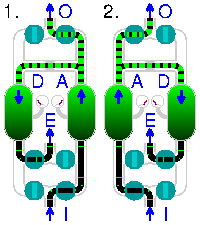
\includegraphics[width=0.75\textwidth]{figuras/fig_15_1_psa.pdf}
			\caption[Princípio de operação das torres PSA]{Princípio de operação das torres PSA em ciclos alternados de adsorção (A) e regeneração/dessorção (D). I = entrada de ar úmido, O = saída de ar seco, E = exaustão da purga. Fonte: \textit{Pressure swing adsorption principle}, Cmglee, Wikimedia Commons, licença CC BY-SA 4.0.}
			\label{fig:15-1}
		\end{figure}

		\subsection{\textbf{Cinética de Adsorção e Balanço de Massa}}
		
		O Gêmeo Digital modela a Zona de Transferência de Massa (MTZ) para prever a saturação do leito dessecante.
		
		\begin{itemize}
			\item \textbf{Capacidade de Adsorção Dinâmica ($q_d$):} A Equação~\eqref{eq:s15-1} descreve como a capacidade do leito dessecante de reter umidade decai exponencialmente ao longo do ciclo de adsorção, partindo da capacidade de equilíbrio e caindo à medida que a razão entre o tempo já decorrido e o tempo de residência do ar no leito aumenta:
			\begin{equation}\label{eq:s15-1}
q_d = q_{eq} \cdot \exp \left( -k_{ads} \cdot \frac{t_{ads}}{t_{res}} \right)
\end{equation}
			Onde $q_{eq}$ é a capacidade de adsorção em equilíbrio (isoterma do dessecante), $t_{ads}$ o tempo decorrido de adsorção, $t_{res}$ o tempo de residência do ar no leito, e $k_{ads}$ é a constante de taxa de adsorção do material dessecante (obtida experimentalmente, específica da alumina ativada ou peneira molecular empregada; subscrito para não colidir com $k$ do relé IEC 60255 ou o índice de tempo discreto usado nos capítulos de EKF/MPC/PSO). A Figura~\ref{fig:15-2} mostra como um $k_{ads}$ maior — leito mais fino, mais contaminado ou material dessecante degradado — acelera drasticamente a saturação, esgotando a capacidade útil do leito muito antes do fim do ciclo programado.

			\begin{figure}[h!tbp]
				\centering
				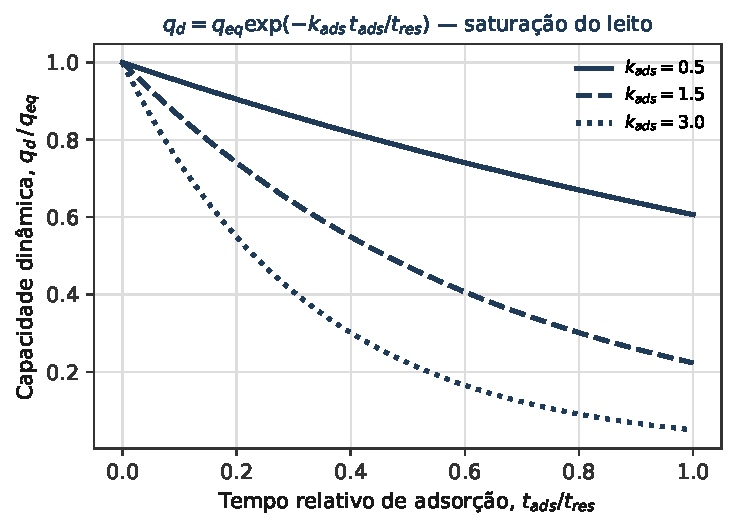
\includegraphics[width=0.60\textwidth]{figuras/fig_15_2_adsorcao.pdf}
				\caption[Capacidade de adsorção dinâmica normalizada]{Capacidade de adsorção dinâmica normalizada em função do tempo relativo de adsorção, para diferentes constantes de taxa $k_{ads}$.}
				\label{fig:15-2}
			\end{figure}

			\item \textbf{Vazão de Purga de Regeneração ($\dot{m}_{purge}$):}
			Calculada pela Equação~\eqref{eq:s15-2} para compensar a histerese de adsorção com o fator $\phi$:
			\begin{equation}\label{eq:s15-2}
\dot{m}_{purge} = \dot{m}_{in} \cdot \left( \frac{P_{low}}{P_{high}} \right) \cdot \phi
\end{equation}
			
			\item \textbf{Balanço de Umidade Acumulada:} A Equação~\eqref{eq:s15-3} encadeia três grandezas: primeiro a queda na razão de umidade entre entrada e saída do leito ($\Delta W$), depois a vazão mássica de água efetivamente retida ($\dot{m}_{water}$, obtida multiplicando $\Delta W$ pela vazão de ar seco), e por fim a massa total de água acumulada no leito ($M_{ads}$) integrando essa vazão ao longo de todo o ciclo de adsorção — usada para prever quando o leito se aproxima da saturação:
			\begin{equation}\label{eq:s15-3}
			\begin{aligned}
				\Delta W &= W_{in} - W_{out} \\[4pt]
				\dot{m}_{water} &= \dot{m}_a \cdot (W_{in} - W_{out}) \\[4pt]
				M_{ads}(t) &= \int_0^{t_{cycle}} \dot{m}_{water} \, dt
			\end{aligned}
\end{equation}
		\end{itemize}
		
		\subsection{\textbf{Termodinâmica do Secador de Tambor Rotativo (HOC)}}
		
		Este subsistema utiliza o calor residual do estágio de alta pressão ($HP$) para regenerar a matriz dessecante.
		
		\begin{itemize}
			\item \textbf{Efetividade de Regeneração Térmica ($\eta_{reg}$):} Mesmo princípio de efetividade usado nos trocadores de calor do documento: a Equação~\eqref{eq:s15-4} compara a queda real de temperatura do ar de regeneração com a máxima queda possível, limitada pela temperatura ambiente:
			\begin{equation}\label{eq:s15-4}
\eta_{reg} = \frac{T_{reg,in} - T_{reg,out}}{T_{reg,in} - T_{amb}}
\end{equation}
			
			\item \textbf{Velocidade de Rotação Crítica ($\omega_{drum}$):}
			Ajustada dinamicamente pela Equação~\eqref{eq:s15-5} para evitar o \textit{carry-over} de umidade:
			\begin{equation}\label{eq:s15-5}
\omega_{drum} \propto \frac{\dot{m}_a}{\rho_a \cdot C_p \cdot \Delta T_{ads}}
\end{equation}
		\end{itemize}

		\subsection{\textbf{Aproveitamento de Calor Rejeitado na Regeneração}}
		O ciclo HOC já aproveita o calor residual do próprio ar de descarga do estágio HP para aquecer o dessecante, mas esse não é o único calor rejeitado disponível na planta: o aftercooler (Equação~\eqref{eq:s14-2}), o resfriador de óleo (Capítulo de Sistema de Lubrificação e Gestão Térmica) e agora a exaustão forçada do invólucro do pacote (Equação~\eqref{eq:s2-2}) rejeitam calor de baixa/média qualidade que hoje é simplesmente descartado para o ambiente ou para a água de resfriamento. Recuperar parte desse calor para pré-aquecer o ar de regeneração reduz diretamente a potência elétrica que o aquecedor resistivo precisa fornecer.
		\begin{itemize}
			\item \textbf{Calor Residual Disponível para Recuperação ($\dot{Q}_{\text{disp}}$):} A soma das rejeições térmicas das correntes candidatas a um trocador de recuperação de calor, pela Equação~\eqref{eq:s15-10}:
			\begin{equation}\label{eq:s15-10}
\dot{Q}_{\text{disp}} = \dot{Q}_{\text{aftercooler}} + \dot{Q}_{\text{óleo}} + \dot{Q}_{\text{hood}}
\end{equation}
			\item \textbf{Potência do Aquecedor com Recuperação:} A Equação~\eqref{eq:s15-11} reduz a demanda do aquecedor elétrico de regeneração na proporção do calor efetivamente recuperado, limitada pela efetividade do trocador de recuperação ($\epsilon_{\text{recup}}$, mesma definição de efetividade da Equação~\eqref{eq:s15-4}) e nunca abaixo de zero:
			\begin{equation}\label{eq:s15-11}
\dot{W}_{\text{heater,real}} = \max\left(0,\; \dot{W}_{\text{heater,nom}} - \epsilon_{\text{recup}} \cdot \dot{Q}_{\text{disp}}\right)
\end{equation}
			Substituindo $\dot{W}_{\text{heater}}$ por $\dot{W}_{\text{heater,real}}$ na Equação~\eqref{eq:s15-6}, o Gêmeo Digital quantifica em tempo real quanto a recuperação de calor está reduzindo o $SEC_{dry}$ — e pode sinalizar quando o trocador de recuperação está subdimensionado ou incrustado, caso $\epsilon_{\text{recup}}$ medido caia abaixo do valor de projeto sem justificativa de carga térmica.
		\end{itemize}

		\subsection{\textbf{Matriz de Diagnóstico de Falhas}}
		A Tabela~\ref{tab:15-1} relaciona as falhas típicas do secador PSA/tambor rotativo (saturação do leito, falha de chaveamento, degradação térmica e desgaste mecânico) aos seus indicadores primários e à ação prescrita pelo Gêmeo Digital.
		\begin{table}[h!tbp]
			\centering
			\resizebox{\textwidth}{!}{
			\renewcommand{\arraystretch}{1.5}
			\begin{tabular}{llll}
				\toprule
				\textbf{Falha} & \textbf{Indicador Primário} & \textbf{Causa Provável} & \textbf{Ação Digital Twin} \\ \midrule
				Breakthrough & $\uparrow PDP$ & Saturação / Vazão $\uparrow$ & Redução de Carga \\
				Falha Chaveamento & $\Delta P$ Constante & Válvula Solenoide & Alarme Redundância \\
				Degradação Térmica & $\downarrow \Delta T$ Reg. & Envelhecimento (Fouling) & Recalibração $HI_{dryer}$ \\
				Desgaste Tambor & $\uparrow$ Torque Motor & Atrito nos Selos & Manutenção Preditiva \\ \bottomrule
			\end{tabular}
			}
			\caption[Matriz de falhas do secador PSA e do tambor rotativo]{Matriz de diagnóstico de falhas do secador PSA e do tambor rotativo (HOC).}
			\label{tab:15-1}
		\end{table}
		
		\subsection{\textbf{Indicadores Globais de Performance (KPIs)}}
		
		\begin{itemize}
			\item \textbf{Consumo Energético Específico ($SEC_{dry}$):} A Equação~\eqref{eq:s15-6} soma a potência do aquecedor de regeneração e a potência do motor do tambor rotativo, e divide pela vazão de ar seco produzida — o custo energético de secar cada quilograma de ar:
			\begin{equation}\label{eq:s15-6}
SEC_{dry} = \frac{\dot{W}_{heater} + \dot{W}_{drum}}{\dot{m}_{dry}}
\end{equation}

			\item \textbf{Índice de Saúde do Dessecante ($HI_{des}$):} A Equação~\eqref{eq:s15-7} multiplica duas razões normalizadas — perda de carga nominal sobre perda de carga real, e ponto de orvalho alvo sobre ponto de orvalho real — de modo que o índice se degrada tanto se o leito colmatar (aumentando $\Delta P_{real}$) quanto se perder capacidade de secagem (piorando $PDP_{real}$). A razão de ponto de orvalho precisa ser calculada em \textbf{Kelvin}, não em Celsius: como o $PDP$ é negativo na convenção deste documento (ex.: $-40\,^{\circ}$C na Classe 2), tomar a razão diretamente em Celsius inverte o sentido do índice — um $PDP_{real}$ pior (mais próximo de $0\,^{\circ}$C ou positivo) produziria um $HI_{des}$ \textit{maior}, o oposto do pretendido. A conversão ($+273{,}15$) é, portanto, obrigatória:
			\begin{equation}\label{eq:s15-7}
HI_{des} = \frac{\Delta P_{nom}}{\Delta P_{real}} \cdot \frac{PDP_{target} + 273{,}15}{PDP_{real} + 273{,}15}
\end{equation}

			\item \textbf{Perda de Eficiência por Purga ($\eta_{purge}$):} Todo o ar de purga usado para regenerar a torre saturada (Equação~\eqref{eq:s15-2}) é ar já comprimido a alto custo energético e depois descartado sem realizar trabalho útil na planta — em secadores PSA a frio, tipicamente entre 10\% e 18\% de toda a produção do compressor. A Equação~\eqref{eq:s15-9} expressa essa perda como uma eficiência: a fração da vazão total produzida que efetivamente chega ao consumidor final, descontada a purga:
			\begin{equation}\label{eq:s15-9}
\eta_{purge} = 1 - \frac{\dot{m}_{purge}}{\dot{m}_{total}}
\end{equation}
			O Gêmeo Digital deve reportar $\eta_{purge}$ junto ao $SPC$ (Equação~\eqref{eq:s11-11}): um SPC aparentemente saudável pode mascarar uma purga excessiva — por exemplo, um ciclo de regeneração mal ajustado ou uma válvula solenoide vazando entre torres — que já está sendo paga em consumo elétrico antes mesmo de chegar ao consumidor.
		\end{itemize}
		
		\vspace{1em}
		\hrule
		\vspace{1em}
		
		\textbf{Diretriz Técnica Final:} A otimização da purga é realizada em tempo real para minimizar perdas operacionais, pela Equação~\eqref{eq:s15-8}:
		\begin{equation}\label{eq:s15-8}
\boxed{\dot{m}_{purge,opt} = f(W_{in}, \dot{m}_a, P_{in})}
\end{equation}
	
	
\clearpage
\section{Distribuição e Armazenamento (Header e Vasos Pulmão)}

Nesta etapa, o Gêmeo Digital gerencia a integração de múltiplos compressores operando em paralelo e a distribuição do ar comprimido para os diferentes setores da unidade offshore. O sistema utiliza uma lógica de controle escalonada para garantir que, em cenários de perda de geração ou vazamentos críticos, o suprimento para os sistemas de segurança seja preservado através do fechamento seletivo de ramais.

\subsection{Dinâmica de Fluxo e Header de Distribuição Setorizada}

O header principal ramifica-se em três linhas com prioridades distintas. O Gêmeo Digital monitora a pressão no vaso pulmão ($P_{tank}$) e comanda válvulas de isolamento automáticas baseadas em setpoints de segurança:

\begin{itemize}
	\item \textbf{Linha de Emergência (Instrumentação):} Prioridade Máxima. Alimenta sistemas de segurança e válvulas ESD. É a última linha a ser isolada para garantir a integridade da planta.
	\item \textbf{Linha de Processo:} Prioridade Média. Alimenta a produção e extração. É isolada quando a pressão atinge o nível de alerta crítico para preservar o inventário.
	\item \textbf{Linha de Serviços (Utilidades):} Prioridade Baixa. Alimenta ferramentas pneumáticas e limpeza. É a primeira linha a sofrer restrição (\textit{load shedding}).
	\item \textbf{Balanço de Massa com Variáveis de Estado ($\delta$):} A vazão total da frota se reparte entre as três linhas de prioridade conforme o estado das válvulas de isolamento, pela Equação~\eqref{eq:s16-1}:
	\begin{equation}\label{eq:s16-1}
\dot{m}_{total} = \sum_{i=1}^{N_{\text{frota}}} \dot{m}_{comp,i} = \dot{m}_{emerg} + \delta_{proc} \cdotp \dot{m}_{proc} + \delta_{serv} \cdotp \dot{m}_{serv}
\end{equation}
	Onde $N_{\text{frota}}$ é o número de compressores ativos na frota (subscrito para não colidir com $N_{\text{rot}}$, rotação em RPM nos capítulos de rolamentos) e $\delta \in \{0, 1\}$ representa o estado (aberto/fechado) da válvula de isolamento de cada ramal.
\end{itemize}

\subsection{Pulsação de Pressão e Ressonância Acústica na Tubulação}
O balanço de massa da Equação~\eqref{eq:s16-1} descreve o nível médio de pressão no header, mas não captura as flutuações de alta frequência geradas pela passagem dos lóbulos do rotor ($f_{bp}$, Equação~\eqref{eq:s9-8}) e pelo engrenamento (GMF). Em compressores de deslocamento positivo, essas pulsações se propagam pela tubulação de descarga e podem excitar um modo acústico do sistema vaso-tubulação, risco não coberto pelo balanço de massa quase-estático já modelado.
\begin{itemize}
	\item \textbf{Frequência Acústica Natural (Ressonador de Helmholtz):} O trecho de tubulação conectando o compressor ao vaso pulmão se comporta como um ressonador de Helmholtz, cuja frequência natural é dada pela Equação~\eqref{eq:s16-2}:
	\begin{equation}\label{eq:s16-2}
 f_H = \frac{c}{2\pi} \sqrt{\frac{A_{\text{tubo}}}{V_{\text{tank}} \cdot L_{\text{eff}}}} 
\end{equation}
	Onde $c$ é a velocidade do som no ar comprimido (função de $T$ e da umidade), $A_{\text{tubo}}$ a área da seção do tubo, $V_{\text{tank}}$ o volume do vaso pulmão e $L_{\text{eff}}$ o comprimento efetivo do trecho (comprimento físico acrescido de correção de extremidade).
	\item \textbf{Critério de Risco de Ressonância:} O Gêmeo Digital compara $f_H$ com as frequências de excitação mecânica conhecidas do trem de compressão, pelo critério da Equação~\eqref{eq:s16-3}:
	\begin{equation}\label{eq:s16-3}
 \text{Risco de Ressonância se} \quad \left| \frac{f_H - f_{bp}}{f_H} \right| < 0.10 \quad \text{ou} \quad \left| \frac{f_H - GMF}{f_H} \right| < 0.10 
\end{equation}
	seguindo a mesma lógica de margem de separação usada na análise rotordinâmica dos eixos (Equação~\eqref{eq:s8-6}, Capítulo de Dinâmica de Transmissão), mas aplicada ao domínio acústico da tubulação, conforme a prática de projeto da API 618 \cite{api618}.
	\item \textbf{Consequência Operacional:} Ressonância sustentada amplifica a amplitude de pulsação na linha, acelerando fadiga em conexões soldadas e instrumentação de pressão, e pode ser confundida em campo com falha mecânica do próprio compressor — daí a necessidade de o modelo distinguir explicitamente pulsação acústica de vibração de origem mecânica.
	\item \textbf{Mitigação de Projeto:} Quando o critério da Equação~\eqref{eq:s16-3} indica risco, a resposta não é apenas operacional — a mesma prática da API 618 \cite{api618} que fundamenta o critério de risco trata do acessório físico correspondente: um amortecedor de pulsação (\textit{volume bottle}), instalado o mais próximo possível da descarga do compressor, que desloca $f_H$ deliberadamente para fora da faixa de excitação ao alterar o volume efetivo $V_{\text{tank}}$ e o comprimento $L_{\text{eff}}$ da Equação~\eqref{eq:s16-2}. É uma decisão de projeto, não de operação — mas o Gêmeo Digital deve registrar sua presença (ou ausência) como parâmetro fixo do sistema ao avaliar a Equação~\eqref{eq:s16-3} para cada unidade da frota.
\end{itemize}

\subsection{Lógica Escalonada de Alarmes e Proteção}

O Gêmeo Digital atua preventivamente, escalonando ações conforme a pressão do vaso pulmão declina devido a falhas na geração ou demanda excessiva:

\begin{itemize}
	\item \textbf{Nível 1 (Alerta de Pressão Baixa - $P_{L}$):} Disparo de alarme visual/sonoro e verificação automática do status de partida dos compressores em \textit{standby}.
	\item \textbf{Nível 2 (Corte de Serviços - $P_{LL}$):} Fechamento automático da válvula da Linha de Serviços ($\delta_{serv} = 0$) para estancar a queda de pressão.
	\item \textbf{Nível 3 (Corte de Processo - $P_{LLL}$):} Fechamento da válvula da Linha de Processo ($\delta_{proc} = 0$). O inventário de ar restante é dedicado exclusivamente à Emergência.
	\item \textbf{Nível 4 (Trip de Emergência - $P_{ESD}$):} Atingimento da pressão mínima de segurança para instrumentação, disparando o ESD (\textit{Emergency Shutdown}) da planta.
\end{itemize}

\subsection{Modelagem Termodinâmica e Autonomia}

\begin{itemize}
	\item \textbf{Taxa de Variação de Pressão ($\frac{dP}{dt}$):}
	Calculada em tempo real pela Equação~\eqref{eq:s16-4} para prever o comportamento da rede:
	\begin{equation}\label{eq:s16-4}
\frac{dP}{dt} = \frac{R \cdotp T}{V_{tank}} \cdotp \left( \sum \dot{m}_{in} - \sum \dot{m}_{out} \right)
\end{equation}
	\item \textbf{Tempo de Autonomia por Setor ($t_{to\_cut}$):}
	Predição do tempo restante, pela Equação~\eqref{eq:s16-5}, antes que o sistema atinja o próximo nível de corte:
	\begin{equation}\label{eq:s16-5}
t_{to\_cut} = \frac{V_{tank} \cdotp (P_{actual} - P_{threshold})}{\dot{V}_{demand} \cdotp P_{atm}}
\end{equation}
\end{itemize}

\subsection{Matriz de Diagnóstico de Falhas (Frota e Distribuição)}

A operação com múltiplos compressores em paralelo introduz riscos específicos de frota (refluxo, sobrepressão por travamento de PSV, falha de sequenciamento) que a Tabela~\ref{tab:16-1} resume junto ao indicador primário e à ação correspondente do Gêmeo Digital.
\begin{table}[h!tbp]
\centering
\noindent\resizebox{\textwidth}{!}{
	\begin{tabular}{l l l l}
		\toprule
		\textbf{Falha} & \textbf{Indicador Primário} & \textbf{Causa Provável} & \textbf{Ação Digital Twin} \\ \midrule
		\textbf{PSV Travada (Fechada)} & $P > P_{set}$ sem alívio & Corrosão / Travamento & Trip de Emergência da Frota \\
		\textbf{Falha de Sequenciamento} & $\downarrow P_{tank}$ (Standby ativo) & Erro de lógica / Partida falha & Comando forçado de partida \\
		\textbf{Vazamento Crítico} & $\frac{dP}{dt} \ll 0$ (Gradiente alto) & Ruptura de linha principal & Antecipação do corte de ramais \\
		\textbf{Falha na Check Valve} & $\dot{m}_i < 0$ (Refluxo) & Quebra da portinhola & Isolamento da Unidade $i$ \\
		\textbf{PSV Travada (Aberta)} & Disparo prematuro & Fadiga da mola / Sujeira & Alarme de perda de eficiência \\ \bottomrule
	\end{tabular}
}
\caption[Matriz de diagnóstico de falhas de frota e distribuição]{Matriz de diagnóstico de falhas de frota e distribuição (header e vasos pulmão).}
\label{tab:16-1}
\end{table}

\subsection{Indicadores Globais de Performance (KPIs)}

\begin{itemize}
	\item \textbf{Índice de Confiabilidade de Pressão ($R_p$):} Porcentagem do tempo de operação em que $P_{tank} > P_{LL}$.
	\item \textbf{Eficiência de Resposta de Carga ($E_{resp}$):} Tempo decorrido entre a detecção da queda de pressão e a efetivação do corte do ramal.
	\item \textbf{Consumo Específico da Frota ($SPC_{fleet}$):} Cada $\dot{V}_{free\_air,i}$ é a vazão da unidade $i$ já convertida às condições de referência da Equação~\eqref{eq:s11-12} — sem essa normalização por máquina, a soma da frota misturaria vazões medidas em condições de sucção potencialmente distintas entre unidades, como soma a Equação~\eqref{eq:s16-6}:
	\begin{equation}\label{eq:s16-6}
SPC_{fleet} = \frac{\sum_{i=1}^{N_{\text{frota}}} \dot{W}_{tot,i}}{\sum_{i=1}^{N_{\text{frota}}} \dot{V}_{free\_air,i}} \quad [\text{kW} \cdotp \text{s} \cdotp \text{m}^{-3}]
\end{equation}
\end{itemize}

\vspace{1em}
\hrule
\vspace{1em}

\textbf{Diretriz Técnica Final:} A integridade do sistema depende da correta calibração dos níveis de alarme e da resposta das válvulas de isolamento. A falha da PSV em não abrir permanece como o risco mais crítico de sobrepressão, exigindo que o Gêmeo Digital monitore o gradiente positivo de pressão em relação à capacidade de alívio nominal, pela Equação~\eqref{eq:s16-7}:

\begin{equation}\label{eq:s16-7}
\boxed{\dot{m}_{leak} = \frac{V_{tank}}{R \cdotp T} \cdotp \left( \frac{dP}{dt} \right)_{static}}
\end{equation}



\clearpage
\section{Modelagem Digital Twin: IA, Exergia e Sustentabilidade}

A modelagem do Gêmeo Digital consolida o fluxo de dados massivo proveniente da rede de automação e do PI System, integrando variáveis críticas de processo com algoritmos de Inteligência Artificial e termodinâmica de segunda lei. O sistema monitora a performance mecânica, a qualidade do ar e o impacto ambiental em tempo real.

\subsection{Aquisição de Dados e Variáveis Críticas de Automação}

O Gêmeo Digital processa o vetor de estado $z(t)$ extraído continuamente da instrumentação de campo. As variáveis fundamentais para a fidelidade do modelo e proteção dos equipamentos clientes são:

\begin{itemize}
	\item \textbf{Pressões ($P$):} Sucção, descarga de estágios e pressão no header de distribuição.
	\item \textbf{Temperaturas ($T$):} Entrada e saída de compressores e trocadores de calor.
	\item \textbf{Diferenciais de Pressão ($\Delta P$):} Queda de carga em filtros e secadores (indicadores de colmatação).
	\item \textbf{Vazão ($\dot{m}$):} Medição direta ou estimada para balanço de massa e energia.
	\item \textbf{Ponto de Orvalho ($T_{dp}$):} Variável crítica para conformidade com a classe de umidade contratada da ISO 8573-1 \cite{iso8573}, evitando condensação e corrosão nos equipamentos clientes.
	\item \textbf{Vetor de Entrada Global ($z$):} As variáveis acima se organizam no vetor de entrada da Equação~\eqref{eq:s17-1}:
	\begin{equation}\label{eq:s17-1}
z = [P, T, \Delta P, \dot{m}, T_{dp}, I, V]^T
\end{equation}
\end{itemize}

\subsection{IA para Detecção Prematura e Qualidade do Ar}

Utilizando redes neurais do tipo Autoencoders e LSTMs, o Gêmeo Digital identifica desvios sutis que precedem falhas operacionais ou perda de qualidade do ar (umidade excessiva).

\begin{itemize}
	\item \textbf{Erro de Reconstrução ($E_{rec}$):}
	O modelo aprende as correlações nominais entre as variáveis. Desvios em $T_{dp}$ ou $\Delta P$ geram um aumento no resíduo da Equação~\eqref{eq:s17-2}:
	\begin{equation}\label{eq:s17-2}
E_{rec} = \sum_{j=1}^{M} (z_j - \hat{z}_j)^2
\end{equation}
	
	\item \textbf{Predição de Breakthrough:} A IA analisa a taxa de variação $\frac{dT_{dp}}{dt}$ para antecipar a saturação do leito dessecante nos secadores PSA antes que o limite normativo seja atingido.
\end{itemize}

\subsection{Otimização de Processos via Exergia}

\textbf{Da entropia à exergia — uma explicação conceitual:} A Segunda Lei da Termodinâmica estabelece que a entropia de um sistema isolado nunca diminui: todo processo real — atrito, transferência de calor sob diferença finita de temperatura, ou um gás escoando livremente por um vazamento — gera entropia ($\dot{S}_{gen} \ge 0$), e esse aumento é irreversível, não há como ``desfazê-lo'' sem gastar ainda mais energia em outro lugar. A Primeira Lei garante que a energia total se conserva (nunca é destruída), mas a Segunda Lei revela algo que a Primeira não enxerga: a \textit{qualidade} dessa energia — sua capacidade de realizar trabalho útil — se degrada continuamente à medida que a entropia aumenta. É exatamente essa perda de qualidade, invisível para um balanço de energia comum, que a \textbf{exergia} foi criada para medir.

Formalmente, exergia é o trabalho útil máximo que poderia ser extraído de um fluxo de energia ou matéria, levando-o reversivelmente até o equilíbrio com o ambiente de referência (pressão e temperatura atmosféricas, $P_0$ e $T_0$). A energia nunca é destruída; a exergia, sim — e a quantidade destruída é diretamente proporcional à entropia gerada pelo processo, $\dot{I} = T_0 \cdot \dot{S}_{gen}$: essa é a mesma relação que abre a Equação~\eqref{eq:s17-3} logo abaixo, destruição de exergia é, literalmente, entropia gerada multiplicada pela temperatura ambiente — uma forma de converter a ``desordem'' termodinâmica (um conceito abstrato, medido em J/K) em uma grandeza concreta e comparável, medida em Watts.

\textbf{Exemplo aplicado a este documento:} um vazamento interno entre os rotores do compressor (a folga $\delta$ discutida nos capítulos anteriores) deixa o ar de alta pressão escoar para uma câmara de baixa pressão sem produzir nenhum trabalho útil. A energia contida nesse ar não desaparece — ela permanece no sistema, agora dissipada como calor e turbulência —, então um balanço de energia convencional não acusaria perda alguma. A exergia é o que revela o prejuízo real: o \textit{potencial} daquele ar pressurizado de realizar trabalho foi destruído de forma permanente, e $\dot{I}$ quantifica exatamente quantos Watts esse potencial valia. É essa mesma unidade (Watts de exergia destruída) que permite comparar, lado a lado e na mesma régua, o vazamento por folga interna, a incrustação no trocador de calor e o atrito no mancal — e assim priorizar qual intervenção realmente devolve mais eficiência à máquina.

O conceito estende a noção de ``energia disponível'' de Gibbs e Keenan, formalizada sob o termo \textit{exergia} por Zoran Rant em 1956 e consolidada como ferramenta de otimização de processos industriais nas décadas seguintes \cite{bejan}.

\begin{itemize}
	\item \textbf{Taxa de Destruição de Exergia ($\dot{I}$):} Formalizada na Equação~\eqref{eq:s17-3} como balanço de exergia entre entrada, saída e trabalho de eixo:
	\begin{equation}\label{eq:s17-3}
\dot{I} = T_0 \cdotp \dot{S}_{gen} = \sum \dot{m}_{in} \psi_{in} - \sum \dot{m}_{out} \psi_{out} - \dot{W}_{shaft}
\end{equation}
	Onde $\psi = (h - h_0) - T_0 \cdotp (s - s_0)$ é a exergia específica de fluxo — o trabalho útil máximo extraível de cada kg de fluido, definida por unidade de massa para poder ser multiplicada pela vazão $\dot{m}$ em cada termo da equação acima (notação de Kotas \cite{bejan}; usa-se $\psi$ em vez de $b$ para não colidir com a largura de dente da engrenagem, usada no modelo de Lewis, e com o expoente de Basquin, usado na Regra de Miner).
	
	\item \textbf{Eficiência Exergética Global ($\eta_{ex}$):}
	O Gêmeo Digital busca maximizar este índice, definido na Equação~\eqref{eq:s17-4}, para garantir a operação próxima ao limite termodinâmico:
	\begin{equation}\label{eq:s17-4}
\eta_{ex} = 1 - \frac{\dot{I}_{comp} + \dot{I}_{cool} + \dot{I}_{dry}}{\dot{W}_{real}}
\end{equation}
\end{itemize}

\subsection{Redução de Consumo e Emissões de GEE}

A redução das emissões de Gases de Efeito Estufa (GEE) é tratada como uma consequência direta da eficiência exergética. O sistema executa uma otimização multiobjetivo para equilibrar performance e sustentabilidade.

\begin{itemize}
	\item \textbf{Taxa de Emissão de $CO_2$ ($\dot{m}_{CO_2}$):} A Equação~\eqref{eq:s17-5} converte a potência elétrica total consumida pelo sistema em massa de $CO_2$ emitida, multiplicando pelo fator de emissão da matriz elétrica local ($EF_{carbon}$, em kg de $CO_2$ por kWh) — quanto mais exergia é destruída (mais potência é necessária para o mesmo trabalho útil), maior essa emissão:
	\begin{equation}\label{eq:s17-5}
\dot{m}_{CO_2} = \dot{W}_{total} \cdotp EF_{carbon} \quad [\text{kg} \cdotp \text{h}^{-1}]
\end{equation}
	
	\item \textbf{Função de Custo Ambiental ($J$):}
	O sistema ajusta setpoints para minimizar $J$, definido na Equação~\eqref{eq:s17-6}:
	\begin{equation}\label{eq:s17-6}
J = w_1 \cdotp \dot{I} + w_2 \cdotp \dot{m}_{CO_2} + w_3 \cdotp (T_{dp} - T_{dp,set})^2
\end{equation}
\end{itemize}

\subsection{Matriz de Diagnóstico, Normas e Sustentabilidade}

A Tabela~\ref{tab:17-1} conecta cada variável crítica de automação ao indicador de IA correspondente, à norma ou risco associado e à ação que o Gêmeo Digital deve tomar automaticamente.
\begin{table}[h!tbp]
\centering
\noindent\resizebox{\textwidth}{!}{
	\begin{tabular}{l l l l}
		\toprule
		\textbf{Variável PI} & \textbf{Indicador IA} & \textbf{Risco / Norma} & \textbf{Ação Gêmeo Digital} \\ \midrule
		\textbf{$T_{dp}$ (Orvalho)} & $\uparrow$ Resíduo & ISO 8573-1 / Corrosão & Antecipar ciclo de secagem \\
		\textbf{$\Delta P$ Filtros} & $\uparrow E_{rec}$ & Perda de Carga & Alarme de manutenção preditiva \\
		\textbf{$P, T$ Estágio} & Desvio de Curva & $\uparrow$ Consumo / $\uparrow$ GEE & Ajuste de carga e rotação \\
		\textbf{$\dot{m}$ (Vazão)} & Balanço de Massa & Vazamento de Inventário & Localizar perda mássica \\ \bottomrule
	\end{tabular}
}
\caption[Matriz de diagnóstico e sustentabilidade do Gêmeo Digital]{Matriz de diagnóstico, normas associadas e ações de sustentabilidade do Gêmeo Digital.}
\label{tab:17-1}
\end{table}

\vspace{1em}
\hrule
\vspace{1em}

\textbf{Diretriz Técnica Final:} A integração do ponto de orvalho como variável crítica garante a proteção dos equipamentos clientes e o atendimento às normas internacionais. O Gêmeo Digital opera no Ponto de Máxima Sustentabilidade, onde a redução de emissões é alcançada pela minimização da geração de entropia, condição formalizada na Equação~\eqref{eq:s17-7}:

\begin{equation}\label{eq:s17-7}
\boxed{\text{Min } \dot{S}_{gen} \implies \text{Min } \dot{m}_{CO_2} \quad \text{com } T_{dp} < T_{dp,limit}}
\end{equation}




\clearpage
\section{Unificação do Modelo Matemático e Matriz Global de Variáveis}

Este capítulo estabelece a síntese definitiva do Gêmeo Digital, integrando a totalidade das equações físicas, modelos estocásticos e algoritmos de inteligência artificial desenvolvidos ao longo deste estudo. A unificação abrange o fluxo completo de energia e massa, desde o relé de proteção no MCC até o header de distribuição final, consolidando a governança de dados para integridade mecânica, eficiência exergética e conformidade normativa.

\subsection{Matriz Abrangente de Variáveis, Localização e Instrumentação}

A observabilidade total do sistema — condição necessária para que o Filtro de Kalman Estendido do Capítulo 21 consiga estimar o estado interno da máquina — é garantida pelo monitoramento combinado de variáveis \textbf{reais}, lidas diretamente de um sensor físico, e \textbf{virtuais} (\textit{soft-sensors}), calculadas pelo modelo a partir das primeiras. A Tabela~\ref{tab:18-1} consolida esse mapeamento completo em seis colunas: o \textbf{ponto} de instalação (rotulado de A a I ao longo do trem de compressão, do MCC ao \textit{header} de distribuição), o \textbf{subsistema} correspondente, a \textbf{grandeza} monitorada, o \textbf{símbolo} usado no equacionamento deste documento, a \textbf{unidade} SI adotada e a \textbf{função} daquela medição no diagnóstico.

Duas leituras dessa tabela são úteis. Na horizontal, ela funciona como especificação de instrumentação: cada linha corresponde a um requisito de projeto verificável na lista de instrumentos da planta. Na vertical, agrupada por ponto, ela revela a densidade de medição de cada subsistema — e é aí que se identificam as lacunas de observabilidade, isto é, os pontos onde o Gêmeo Digital depende inteiramente de inferência por modelo porque não há sensor físico disponível. Essas lacunas não são falhas de projeto: instrumentar diretamente a câmara de compressão de um rotor girando a milhares de RPM é impraticável, e é justamente por isso que o \textit{soft-sensor} existe. Mas elas precisam estar explícitas, porque determinam onde a incerteza do modelo (Capítulo 25) é maior e onde a validação física do PIML (Capítulo 23) é mais crítica.

\begin{table}[h!tbp]
	\centering
	\resizebox{\textwidth}{!}{
		\begin{tabular}{c l l c l l}
			\toprule
			\textbf{Ponto} & \textbf{Localização} & \textbf{Variável} & \textbf{Tag} & \textbf{Unidade} & \textbf{Definição / Função} \\ \midrule
			\textbf{A} & \textbf{MCC / Relé} & Tensão de Linha & $V_L$ & $\text{V}$ & Potencial elétrico de alimentação \\ \cline{3-6} 
			& & Corrente de Fase & $I$ & $\text{A}$ & Carga elétrica do motor principal \\ \cline{3-6} 
			& & Frequência & $f$ & $\text{Hz}$ & Ciclo da rede / Velocidade do VFD \\ \cline{3-6} 
			& & Fator de Potência & $\cos \phi$ & $-$ & Eficiência da conversão elétrica \\
			\textbf{B} & \textbf{Transmissão} & Velocidade Angular & $\omega$ & $\text{rad}\,\cdotp\,\text{s}^{-1}$ & Rotação real do eixo primário \\ \cline{3-6} 
			& & Torque no Eixo & $\tau$ & $\text{N}\,\cdotp\,\text{m}$ & Momento torsor transmitido \\ \cline{3-6} 
			& & Vibração Global & $v_{\text{rms}}$ & $\text{mm}\,\cdotp\,\text{s}^{-1}$ & Severidade vibratória (base API 619/OEM) \\ \cline{3-6}
			& & Tensão no Dente & $\sigma_b$ & $\text{MPa}$ & Esforço na raiz da engrenagem \\
			\textbf{C} & \textbf{Estágio LP} & Pressão Sucção & $P_{s,lp}$ & $\text{bar}$ & Pressão de entrada (atmosférica) \\ \cline{3-6} 
			& & Temp. Descarga & $T_{d,lp}$ & $^{\circ}\text{C}$ & Calor de compressão do 1º estágio \\ \cline{3-6} 
			& & Folga Interna & $\delta_{lp}$ & $\mu\text{m}$ & Espaço residual entre parafusos \\
			\textbf{D} & \textbf{Intercooler} & Temp. Água In & $T_{w,in}$ & $^{\circ}\text{C}$ & Temperatura do fluido de resfriamento \\ \cline{3-6} 
			& & Delta Pressão & $\Delta P_{ic}$ & $\text{bar}$ & Perda de carga no trocador \\ \cline{3-6} 
			& & Vazão Condensado & $\dot{m}_{c}$ & $\text{kg}\,\cdotp\,\text{h}^{-1}$ & Taxa de remoção de umidade \\
			\textbf{E} & \textbf{Estágio HP} & Pressão Descarga & $P_{d,hp}$ & $\text{bar}$ & Pressão final de compressão \\ \cline{3-6}
			& & Temp. Descarga & $T_{d,hp}$ & $^{\circ}\text{C}$ & Temperatura crítica do 2º estágio \\ \cline{3-6}
			& & Folga Interna & $\delta_{hp}$ & $\mu\text{m}$ & Desgaste/Dilatação térmica HP \\ \cline{3-6}
			& & Posição Axial & $\delta_{ax}$ & $\mu\text{m}$ & Desgaste do mancal de escora, precede vibração \\
			\textbf{F} & \textbf{Aftercooler} & Temp. Saída & $T_{ac,out}$ & $^{\circ}\text{C}$ & Temperatura pré-secagem \\
			\textbf{G} & \textbf{Secador PSA} & Ponto de Orvalho & $T_{dp}$ & $^{\circ}\text{C}$ & Umidade residual (ISO 8573-1) \\ \cline{3-6} 
			& & Vazão de Purga & $\dot{m}_{p}$ & $\text{kg}\,\cdotp\,\text{s}^{-1}$ & Ar perdido na regeneração \\
			\textbf{H} & \textbf{Vaso Pulmão} & Pressão Vaso & $P_{tk}$ & $\text{bar}$ & Energia potencial acumulada \\ \cline{3-6} 
			& & Nível Condensado & $L_{tk}$ & $\%$ & Acúmulo de líquido no pulmão \\
			\textbf{I} & \textbf{Header} & Vazão de Demanda & $\dot{m}_{tot}$ & $\text{kg}\,\cdotp\,\text{s}^{-1}$ & Consumo real da unidade offshore \\ \cline{3-6} 
			& & Status Ramal & $\delta_{i}$ & $\text{bin}$ & Lógica de corte (Serviço/Processo) \\ \bottomrule
		\end{tabular}
	}
	\caption[Matriz de variáveis e instrumentação do Gêmeo Digital]{Matriz completa de variáveis e instrumentação do Gêmeo Digital.}
	\label{tab:18-1}
\end{table}

\subsection{Consolidação do Motor de Cálculo Unificado}

O processamento matemático do Gêmeo Digital é executado através da integração de cinco domínios fundamentais, operando em tempo real sobre os dados do PI System:

\textbf{1. Domínio Eletromecânico e Fadiga Estrutural (Pontos A e B):} A Equação~\eqref{eq:s18-1} encadeia os pontos A e B da matriz acima: a potência elétrica trifásica medida no painel ($\dot{W}_{\text{elec}}$) determina o torque no eixo ($\tau_{\text{shaft}}$), que por sua vez alimenta o cálculo de tensão na raiz do dente ($\sigma_b$, mesmo modelo de Lewis da Equação~\eqref{eq:s8-7}) sob a restrição de sincronismo já vista na Equação~\eqref{eq:s8-9}:
\begin{equation}\label{eq:s18-1}
\begin{aligned}
	\dot{W}_{\text{elec}} &= \sqrt{3} \cdotp V_L \cdotp I \cdotp \cos \phi \\[8pt]
	\tau_{\text{shaft}} &= \frac{\dot{W}_{\text{elec}} \cdotp \eta_m}{\omega} \\[8pt]
	\sigma_b &= \frac{F_t}{b \cdotp m \cdotp Y} \cdotp K_v \cdotp K_o \cdotp K_s \quad \text{com} \quad \Delta \theta_{\text{sync}} < \theta_{\text{backlash}}
\end{aligned}
\end{equation}

\textbf{2. Domínio Termoflutuídico e Eficiência de Compressão (Pontos C, D e E):} A Equação~\eqref{eq:s18-2} encadeia os pontos C a E: a eficiência volumétrica ($\eta_v$, função da folga $\delta$) determina a temperatura de descarga real, e ambas alimentam o cálculo do trabalho de compressão somado sobre os dois estágios — a mesma física dos Capítulos de Termodinâmica LP e HP, agora vista como um único bloco de cálculo:
\begin{equation}\label{eq:s18-2}
\begin{aligned}
	\eta_{v} &= 1 - \frac{C_d \cdotp A_{\text{gap}}(\delta) \cdotp \sqrt{2\rho (P_d - P_s)}}{\dot{m}_{\text{th}}} \\[8pt]
	T_{\text{out}} &= T_{\text{in}} \cdotp \left( \frac{P_{\text{out}}}{P_{\text{in}}} \right)^{\frac{n-1}{n}} \\[8pt]
	\dot{W}_{\text{comp}} &= \sum_{i=1}^{2} \left[ \frac{\dot{m}_i \cdotp R \cdotp T_{s,i}}{\eta_{is,i}} \left( \frac{\gamma}{\gamma - 1} \right) \left( \left( \frac{P_{d,i}}{P_{s,i}} \right)^{\frac{\gamma-1}{\gamma}} - 1 \right) \right]
\end{aligned}
\end{equation}

\textbf{3. Domínio de Exergia e Sustentabilidade Ambiental (Global):} A Equação~\eqref{eq:s18-3} retoma a destruição de exergia introduzida na Equação~\eqref{eq:s17-3} — aqui escrita em termos de entropia de fluxo ($s$) de entrada e saída mais a troca de calor com o ambiente — e a propaga para a eficiência exergética global e, a partir dela, para a taxa de emissão de $CO_2$:
\begin{equation}\label{eq:s18-3}
\begin{aligned}
	\dot{I} &= T_0 \left[ \sum (\dot{m}s)_{\text{out}} - \sum (\dot{m}s)_{\text{in}} - \frac{\dot{Q}}{T_{\text{surr}}} \right] \\[8pt]
	\eta_{\text{ex}} &= 1 - \frac{\dot{I}}{\dot{W}_{\text{elec}}} \\[8pt]
	\dot{m}_{\text{CO}_2} &= \dot{W}_{\text{elec}} \cdotp EF_{\text{carbon}} \cdotp (1 - \eta_{\text{ex}})
\end{aligned}
\end{equation}

\textbf{4. Domínio de Qualidade do Ar e Tratamento (Pontos F e G):} A Equação~\eqref{eq:s18-4} reúne a taxa de condensação (mesma forma da Equação~\eqref{eq:s14-3}) com a degradação do coeficiente de troca térmica por incrustação (mesma relação da Equação~\eqref{eq:s10-5}) — os dois mecanismos que juntos determinam se o ar chega seco o suficiente ao secador PSA:
\begin{equation}\label{eq:s18-4}
\begin{aligned}
	\dot{m}_{\text{cond}} &= \dot{m}_a \cdotp (W_{\text{in}} - W_{\text{sat,out}}) \\[8pt]
	\epsilon_{\text{hex}} &= \frac{T_{h,in} - T_{h,out}}{T_{h,in} - T_{c,in}} \implies \frac{1}{U_{\text{real}}} = \frac{1}{U_{\text{clean}}} + R_f
\end{aligned}
\end{equation}

\textbf{5. Domínio de Dinâmica de Inventário e Autonomia (Pontos H e I):} Fechando o motor de cálculo, a Equação~\eqref{eq:s18-5} retoma a dinâmica de pressão do vaso pulmão (mesma forma da Equação~\eqref{eq:s16-4}) e a propaga para o tempo de autonomia até a pressão crítica — a última etapa antes da lógica de alarmes global apresentada a seguir:
\begin{equation}\label{eq:s18-5}
\begin{aligned}
	\frac{dP_{tk}}{dt} &= \frac{R \cdotp T}{V_{tk}} \cdotp (\dot{m}_{\text{in}} - \dot{m}_{\text{out}}) \\[8pt]
	t_{\text{hold}} &= \frac{V_{tk} \cdotp (P_{tk} - P_{\text{crit}})}{\dot{V}_{\text{demand}} \cdotp P_{\text{atm}}}
\end{aligned}
\end{equation}

\subsection{Matriz Global de Alarmes e Lógica de Decisão}

A lógica de proteção e otimização do Gêmeo Digital não se apoia em indicadores isolados, mas na correlação entre grandezas medidas diretamente por sensor e grandezas inferidas pelo modelo. A Tabela~\ref{tab:18-2} organiza essa lógica em cinco colunas: o \textbf{indicador crítico} monitorado; sua \textbf{tag} no sistema de automação; o \textbf{nível} de severidade na convenção ISA \cite{isa51} (H = alarme alto, que exige ação corretiva mas permite operação continuada; HH = desligamento por valor alto; LL = desligamento por valor baixo); a \textbf{condição de gatilho}, isto é, a inequação que o Gêmeo Digital avalia a cada ciclo de varredura; e a \textbf{ação automática} disparada. Note que os quatro primeiros indicadores são grandezas físicas medidas ou calculadas por primeiros princípios, enquanto os três últimos ($E_{\text{rec}}$, $\dot{I}$ e $\dot{m}_{\text{CO}_2}$) são indicadores virtuais que só existem porque há um modelo por trás — é essa combinação que distingue a matriz de um intertravamento convencional.

\begin{table}[h!tbp]
	\centering
	\resizebox{\textwidth}{!}{
		\begin{tabular}{l c c l l}
			\toprule
			\textbf{Indicador Crítico} & \textbf{Tag} & \textbf{Nível} & \textbf{Condição de Gatilho} & \textbf{Ação Automática} \\ \midrule
			\textbf{Ponto de Orvalho} & $T_{dp}$ & \textbf{H} & $T_{dp} > -40^{\circ}\text{C}$ (Classe 2) & Antecipar regeneração PSA / Alarme de classe ISO 8573-1 \\
			\textbf{Pressão do Vaso} & $P_{tk}$ & \textbf{LL} & $P < P_{\text{min}}$ & Corte de Linha de Serviços ($\delta_{\text{serv}}=0$) \\
			\textbf{Tensão no Dente} & $\sigma_b$ & \textbf{H} & $\sigma_b > 0.85 \sigma_{\text{adm}}$ & Limitação de torque via VFD / Unload \\
			\textbf{Vibração Global} & $v_{\text{rms}}$ & \textbf{HH} & $v_{\text{rms}} > v_{\text{trip}}$ (base da máquina) & Trip Mecânico Imediato (ESD) \\
			\textbf{Erro de Reconstrução} & $E_{\text{rec}}$ & \textbf{H} & $E > \tau_{\text{limiar}}$ & Diagnóstico de falha incipiente (Mancais) \\
			\textbf{Destruição Exergética} & $\dot{I}$ & \textbf{H} & $\uparrow$ Tendência ($+15\%$) & Ajuste de setpoint de resfriamento e purga \\
			\textbf{Emissões GEE} & $\dot{m}_{\text{CO}_2}$ & \textbf{H} & $\dot{m} > \dot{m}_{\text{target}}$ & Rebalanceamento de carga da frota \\ \bottomrule
		\end{tabular}
	}
	\caption[Matriz de decisão, alarmes e ações de controle do Gêmeo Digital]{Matriz de decisão, alarmes e ações de controle do Gêmeo Digital.}
	\label{tab:18-2}
\end{table}

Dois gatilhos da Tabela~\ref{tab:18-2} merecem qualificação normativa explícita, porque são frequentemente citados como se fossem números universais — e não são.

O primeiro é o \textbf{ponto de orvalho}. A ISO 8573-1 \cite{iso8573} não estabelece um valor único de $T_{dp}$ para ar comprimido: ela define \textit{classes de pureza}, e a classe de umidade é fixada por um ponto de orvalho sob pressão (PDP) máximo — Classe 1 para $T_{dp} \le -70\,^{\circ}$C, Classe 2 para $T_{dp} \le -40\,^{\circ}$C, Classe 3 para $T_{dp} \le -20\,^{\circ}$C, e assim por diante em direção a valores positivos. O limite de $-40\,^{\circ}$C adotado neste documento corresponde, portanto, à \textbf{Classe 2}, escolhida como requisito de projeto por ser a prática consolidada para ar de instrumentação em unidades offshore, onde a linha pode atravessar regiões não aquecidas e a margem entre o PDP e a menor temperatura de parede precisa ser generosa. Ao especificar essa restrição, o Gêmeo Digital deve registrar não só o valor, mas também o \textbf{ponto de medição} (saída do secador, a jusante do filtro de partículas) e a \textbf{pressão de referência} — um ponto de orvalho medido sob pressão de linha e outro medido após expansão à atmosfera não são a mesma grandeza, e confundi-los produz uma falsa conformidade.

O segundo é o \textbf{limiar de vibração global}. É comum encontrar o valor de $7{,}1\,\text{mm}\cdot\text{s}^{-1}$ aplicado indistintamente a qualquer máquina rotativa, por extensão da família ISO 10816/20816 \cite{iso10816, iso20816}. Essa extensão é indevida no caso presente: a ISO 20816-3 \cite{iso20816}, que substituiu a ISO 10816-3 para máquinas industriais acima de $15\,\text{kW}$, \textbf{exclui explicitamente de seu escopo os compressores rotativos de deslocamento positivo}, citando os compressores de parafuso como exemplo. A razão é física, não burocrática: a assinatura vibratória de um compressor de parafuso é dominada pela frequência de passagem de lóbulos e por pulsação de gás na descarga — componentes que elevam a vibração global sem que isso represente, por si só, degradação mecânica. Um limiar calibrado para turbomáquinas rejeitaria máquinas saudáveis e, o que é pior, poderia mascarar uma degradação real que se manifeste abaixo dele.

O critério correto para $v_{\text{trip}}$ vem de três fontes, nesta ordem de precedência: (i) o valor contratual de aceitação e alarme definido pela API 619 \cite{api619} e pelos requisitos do fabricante (OEM) para aquela carcaça específica; (ii) a \textbf{linha de base da própria máquina}, levantada no comissionamento sob condição de carga conhecida e usada como referência de tendência; e (iii) quando o componente e a montagem se enquadrarem no escopo (o motor elétrico de acionamento, por exemplo, é uma máquina industrial coberta pela ISO 20816-3), o critério da norma aplicado apenas àquele componente. Essa é, aliás, a filosofia do próprio Gêmeo Digital: o desvio relevante é o afastamento da assinatura individual da máquina, não a ultrapassagem de um número tabelado por uma norma que nunca a teve em vista.

\subsection{Sensores Portáteis e Wireless: Complemento à Instrumentação Fixa}

A Tabela~\ref{tab:18-1} assume, em todas as suas linhas, um sensor \textbf{permanentemente instalado} — cabeado até o sistema de automação, amostrando em taxa constante. Essa é a premissa correta para qualquer grandeza que alimente o intertravamento da Tabela~\ref{tab:18-2} ou o ciclo de predição-correção do EKF em tempo real (Equação~\eqref{eq:s21-4}), mas não é a única forma de instrumentação que um Gêmeo Digital pode consumir. Duas categorias de sensor \textbf{não permanente} complementam a matriz fixa sem substituí-la: o instrumento \textbf{portátil}, operado por um técnico em rondas periódicas (analisador de vibração de mão, câmera termográfica portátil, detector ultrassônico de vazamento de ar comprimido), e o nó \textbf{wireless} de retrofit — um sensor sem fio, alimentado por bateria, instalado temporária ou permanentemente num ponto que não justificava o custo de cabeamento até o painel (WirelessHART e ISA100.11a são os dois protocolos consolidados para esse retrofit industrial, ambos padronizados internacionalmente como IEC 62591 e IEC 62734 respectivamente). Ambos preenchem a mesma lacuna: pontos onde uma leitura periódica de baixo custo já entrega valor diagnóstico suficiente, sem justificar uma instalação permanente.

A Tabela~\ref{tab:18-3} lista os casos de uso mais diretos para este trem de compressão, todos complementares a um ponto já existente na Tabela~\ref{tab:18-1}, nunca substitutos de uma medição que já alimenta o intertravamento.

\begin{table}[h!tbp]
	\centering
	\resizebox{\textwidth}{!}{
		\begin{tabular}{l l l l}
			\toprule
			\textbf{Sensor} & \textbf{Ponto/grandeza complementada} & \textbf{Modo} & \textbf{Uso} \\ \midrule
			Analisador de vibração de mão & $v_{\text{rms}}$ (ponto B) & Portátil, ronda periódica & Validação cruzada do acelerômetro fixo; pontos sem acelerômetro \\
			Câmera/pistola termográfica & Carcaças, mancais, painel elétrico & Portátil, ronda periódica & Ponto quente incipiente fora da matriz fixa \\
			Detector ultrassônico de vazamento & Header e ramais (ponto I) & Portátil, ronda periódica & Perda não contabilizada em $\dot{m}_{tot}$ \\
			Contador de partículas de óleo & Circuito de lubrificação & Portátil, amostragem pontual & Complementa a série ISO 4406 já periódica (Cap. 12) \\
			Nó \textit{wireless} de vibração/temperatura & Pontos sem cabeamento viável & Wireless, retrofit & Cobertura de lacuna sem custo de cabeamento novo \\ \bottomrule
		\end{tabular}
	}
	\caption[Instrumentação portátil e wireless complementar à matriz fixa]{Instrumentação portátil e wireless complementar à matriz fixa da Tabela~\ref{tab:18-1}.}
	\label{tab:18-3}
\end{table}

O ciclo de predição-correção do EKF (Equação~\eqref{eq:s21-4}) já lida naturalmente com a irregularidade temporal dessas leituras — a etapa de predição é parametrizada pelo intervalo $\Delta t$ decorrido desde a última medição, seja ele constante (sensor fixo) ou variável (ronda semanal, nó \textit{wireless} de baixa taxa de amostragem para economizar bateria). O que o ciclo \textbf{não} ajusta sozinho é a confiança relativa depositada em cada leitura: uma medição portátil carrega ruído adicional que a fixa não tem — variabilidade de posicionamento da sonda entre rondas, ausência de um ponto de fixação calibrado, e, no caso \textit{wireless}, latência e perda ocasional de pacote. A covariância de ruído de medição $\mathcal{R}$ da Equação~\eqref{eq:s21-1} deve refletir essa diferença, inflada por um fator $\kappa_{\text{port}}$ em relação ao mesmo canal medido de forma fixa, conforme a Equação~\eqref{eq:s18-6}:

\begin{equation}\label{eq:s18-6}
\mathcal{R}_{\text{port}} = \kappa_{\text{port}} \cdot \mathcal{R}_{\text{fixo}}, \qquad \kappa_{\text{port}} > 1
\end{equation}

Ignorar essa inflação — tratar uma leitura de ronda mensal como se tivesse a mesma confiabilidade de um sensor fixo amostrado a cada segundo — tem o mesmo efeito diagnosticado pelo NIS da Equação~\eqref{eq:s21-7}: o filtro passa a confiar demais numa medição ruidosa, e a estimativa diverge da realidade de forma silenciosa, sem que nenhum alarme dispare.

\vspace{1em}
\hrule
\vspace{1em}

\textbf{Diretriz Técnica Final:} A unificação matemática, formalizada na Equação~\eqref{eq:s18-7}, permite que o Gêmeo Digital opere em um ponto de ótimo multiobjetivo, onde a segurança operacional é a restrição fundamental e a sustentabilidade é a meta de performance:

\begin{equation}\label{eq:s18-7}
\begin{aligned}
	\text{Minimizar } J &= \int_{t}^{t+\Delta t} \left( \sum \dot{I} + \beta \sum \dot{m}_{\text{CO}_2} \right) \, dt \\[10pt]
	\text{Sujeito a: } & \begin{cases} T_{dp} \le T_{dp,\text{limit}} \quad (\text{Qualidade}) \\ \sigma_{b} < \sigma_{\text{adm}} \quad (\text{Integridade}) \\ P_{tk} \ge P_{\text{crit}} \quad (\text{Disponibilidade}) \\ \Delta \theta_{\text{sync}} < \theta_{\text{backlash}} \quad (\text{Sincronismo}) \end{cases}
\end{aligned}
\end{equation}

A inflação de $\mathcal{R}$ da Equação~\eqref{eq:s18-6} completa essa unificação num eixo que as quatro restrições anteriores não cobrem: a \textbf{origem} do dado, não só o seu valor. Um Gêmeo Digital que trata uma leitura de ronda mensal e uma leitura de sensor fixo amostrada a cada segundo com a mesma covariância de medição está, na prática, inflando artificialmente sua própria confiança — o mesmo risco silencioso que o NIS da Equação~\eqref{eq:s21-7} existe para detectar.

\clearpage
\thispagestyle{empty}
\phantomsection
\addcontentsline{toc}{part}{II\hspace{1em}Metodologia do Gêmeo Digital e Equacionamento Integrado}
\vspace*{\fill}
\begin{center}
	{\Huge\bfseries PARTE II}\\[2em]
	{\huge\bfseries Metodologia do Gêmeo Digital e Equacionamento Integrado}
\end{center}
\vspace*{\fill}
\clearpage

\clearpage
\section{Modelos de Solução, Acompanhamento e Redução de Dimensionalidade}

Este capítulo descreve a engenharia de integração do Gêmeo Digital, detalhando como o vasto equacionamento multidisciplinar é fundido em um motor de inferência robusto e como a complexidade de dados é tratada para diagnósticos de alta fidelidade. A abordagem proposta transcende o monitoramento convencional ao integrar modelos de primeira ordem com algoritmos de aprendizado profundo.

\subsection{Integração Híbrida: Physics-Informed Machine Learning (PIML)}

Para integrar as equações de termodinâmica, exergia e fadiga em um único modelo de solução, a abordagem adotada é o \textbf{PIML}. Diferente de modelos puramente estatísticos (caixa-preta), o PIML utiliza as leis da física como restrições fundamentais no treinamento e na execução dos algoritmos.

\begin{enumerate}
	\item \textbf{Estrutura do Modelo:}
	As equações diferenciais e algébricas (DAEs) desenvolvidas nos capítulos anteriores são incorporadas diretamente à função de perda ($Loss$) do modelo de inteligência artificial. A Equação~\eqref{eq:s19-1} soma dois termos ponderados: $L_{\text{data}}$, o erro convencional contra os dados medidos, e $L_{\text{physics}}$, a penalidade por violar as leis físicas — os pesos $\omega_1$ e $\omega_2$ controlam o equilíbrio entre ``confiar nos dados'' e ``confiar na física'':
	\begin{equation}\label{eq:s19-1}
 L_{\text{total}} = \omega_1 L_{\text{data}} + \omega_2 L_{\text{physics}}
\end{equation}

	\item \textbf{Componente Físico ($L_{\text{physics}}$):}
	Este termo garante que o modelo respeite o balanço de massa e a Segunda Lei da Termodinâmica, penalizando predições que violem a conservação de energia. A Equação~\eqref{eq:s19-2} soma dois resíduos ao quadrado: o desequilíbrio entre vazão de entrada, saída e variação de massa acumulada (violação da conservação de massa), e a diferença entre o trabalho de compressão previsto e o trabalho termodinâmico teórico (violação da física do processo):
	\begin{equation}\label{eq:s19-2}
 L_{\text{physics}} = \| \dot{m}_{\text{in}} - \dot{m}_{\text{out}} - \frac{dm}{dt} \|^2 + \| \dot{W}_{\text{comp}} - \dot{W}_{\text{th}} \|^2
\end{equation}
	
	\item \textbf{Vantagem Operacional:}
	O modelo torna-se resiliente a sensores ruidosos ou falhas parciais de telemetria, pois o conhecimento físico preenche as lacunas de dados, permitindo a estimação de estados não medidos.
\end{enumerate}

\subsection{Redução de Dimensionalidade: O Modelo de Espaço Latente}

Monitorar 28 variáveis simultaneamente introduz a ``maldição da dimensionalidade'' e problemas de colinearidade. O modelo adotado para simplificar esta estrutura sem perda de informação crítica é o \textbf{Autoencoder Variacional (VAE)}.

\begin{itemize}
	\item \textbf{Limitação do PCA:} A Análise de Componentes Principais (PCA) é linear e falha ao capturar relações complexas, como a variação da viscosidade do óleo ou a dinâmica não linear da compressão politrópica.
	\item \textbf{Arquitetura do Autoencoder:}
	\begin{itemize}
		\item \textbf{Encoder ($q_{\phi}$):} Comprime o vetor de 28 variáveis ($z$) em um vetor reduzido ($\ell$) de 3 ou 4 dimensões, denominado Espaço Latente.
		\item \textbf{Bottleneck (Gargalo):} Força a rede a aprender apenas as características essenciais, ou a ``assinatura de saúde'' do compressor.
		\item \textbf{Decoder ($p_{\theta}$):} Reconstrói o vetor original ($\hat{z}$) a partir do espaço latente para validação.
	\end{itemize}
	\item \textbf{Diagnóstico por Resíduo:}
	O acompanhamento é realizado através do vetor de resíduos ($r$) — a Equação~\eqref{eq:s19-3} é simplesmente a diferença absoluta, variável por variável, entre o vetor de entrada real $z$ e a reconstrução $\hat{z}$ que o decoder produz a partir do espaço latente:
	\begin{equation}\label{eq:s19-3}
 r = | z - \hat{z} |
\end{equation}
	Se o resíduo de uma variável específica (ex: $T_{d,hp}$) cresce enquanto as outras permanecem estáveis, o Gêmeo Digital isola a falha naquele componente específico.
\end{itemize}

\subsection{Modelo de Solução: Otimização e Controle Preditivo (MPC)}

Para resolver a função objetivo multiobjetivo em tempo real, o modelo de solução utiliza o \textbf{Controle Preditivo Baseado em Modelo (MPC)} acoplado a algoritmos de otimização heurística.

\begin{enumerate}
	\item \textbf{Fluxo de Solução:}
	O Gêmeo Digital projeta o estado futuro em um horizonte de tempo $H$, buscando a combinação de rotação ($\omega$) e vazão de resfriamento que minimiza a destruição de exergia ($\dot{I}$).
	
	\item \textbf{Função Objetivo Dinâmica:} O MPC minimiza, ao longo do horizonte $H$, a função de custo da Equação~\eqref{eq:s19-4}:
	\begin{equation}\label{eq:s19-4}
 \text{Minimizar } J = \sum_{k=0}^{H} \left[ \dot{I}(k) + \beta \cdotp \dot{m}_{\text{CO}_2}(k) + \gamma \cdotp \Delta u(k)^2 \right] 
\end{equation}
	
	\item \textbf{Restrições de Integridade:}
	A tensão calculada na raiz do dente ($\sigma_b$) atua como uma barreira de segurança: a Equação~\eqref{eq:s19-5} obriga o MPC a rejeitar qualquer solução da função objetivo da Equação~\eqref{eq:s19-4} que projete a tensão acima do limite admissível em qualquer instante $k$ do horizonte de predição — a otimização energética nunca pode violar essa restrição estrutural:
	\begin{equation}\label{eq:s19-5}
 \sigma_b(k) < \sigma_{\text{adm}} \quad \forall k \in [0, H]
\end{equation}
\end{enumerate}

\subsection{Acompanhamento de Performance e Saúde (KPIs de 3ª Geração)}

O acompanhamento evolui de simples leituras de sensores para indicadores sintéticos de alta ordem:

\begin{itemize}
	\item \textbf{Exergetic Health Index (EHI):} Mede a proximidade do sistema em relação à reversibilidade ideal, ponderado pela consistência dos dados. A Equação~\eqref{eq:s19-6} multiplica a razão entre o trabalho mínimo reversível e o trabalho real (a mesma noção de eficiência exergética da Equação~\eqref{eq:s17-4}) por um fator de desconto exponencial no erro de reconstrução do VAE — de modo que o índice só é alto quando a máquina está próxima do ideal termodinâmico \textbf{e} o modelo confia nos dados que sustentam esse cálculo:
	\begin{equation}\label{eq:s19-6}
 EHI = \frac{\dot{W}_{\text{min,rev}}}{\dot{W}_{\text{real}}} \cdotp \exp(-E_{\text{rec}})
\end{equation}
	
	\item \textbf{Remaining Useful Life (RUL) por Acúmulo de Dano (Regra de Miner):} A formulação anterior deste documento estimava o RUL como uma probabilidade adimensional $P(\text{Dano} \ge 1)$, sem unidade de tempo/ciclos e sem base física — não é derivável de nenhuma curva de fadiga real. A substituição fisicamente fundamentada usa a tensão na raiz do dente ($\sigma_b$, já calculada pelo modelo de Lewis na Equação~\eqref{eq:s8-7}, Capítulo de Dinâmica de Transmissão) como entrada de uma contagem de ciclos por \textit{rainflow} sobre o histórico de operação, convertida em dano acumulado pela Regra de Palmgren-Miner \cite{palmgren, miner}, na Equação~\eqref{eq:s19-7}:
	\begin{equation}\label{eq:s19-7}
 D = \sum_{i} \frac{n_i}{N_i(\sigma_i)} 
\end{equation}
	Onde $n_i$ é o número de ciclos observados na amplitude de tensão $\sigma_i$ e $N_i(\sigma_i)$ é o número de ciclos até a falha para essa amplitude, dado pela curva S-N de Basquin \cite{basquin} do material (ou pela curva normativa AGMA 2001 \cite{agma2001} para dentes de engrenagem), pela Equação~\eqref{eq:s19-8}:
	\begin{equation}\label{eq:s19-8}
 \sigma_i^{\,b_f} \cdot N_i = C 
\end{equation}
	com $b_f$ (expoente de Basquin, subscrito para não colidir com a largura de dente $b$ do modelo de Lewis) e $C$ constantes de fadiga do material. Falha é prevista quando $D = 1$. A Figura~\ref{fig:19-1} traça essa curva S-N em escala log-log — cada ponto vermelho representa um par $(\sigma_i, N_i)$ do histórico de ciclos por \textit{rainflow}, e é a soma das razões $n_i/N_i(\sigma_i)$ para todos esses pontos que compõe o dano $D$ da Equação~\eqref{eq:s19-7}.

	\begin{figure}[h!tbp]
		\centering
		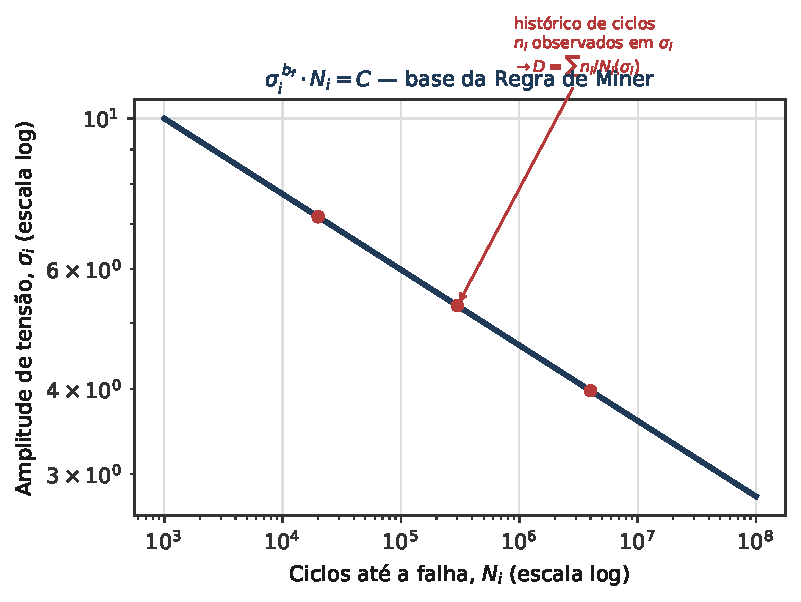
\includegraphics[width=0.60\textwidth]{figuras/fig_20_1_basquin.pdf}
		\caption[Curva S-N de Basquin]{Curva S-N de Basquin (escala log-log) — base da contagem de ciclos da Regra de Palmgren-Miner.}
		\label{fig:19-1}
	\end{figure}

	O RUL — agora expresso em ciclos ou tempo, não em probabilidade adimensional — é obtido, pela Equação~\eqref{eq:s19-9}, projetando o dano restante pela taxa de acúmulo recente $\dot{D}$, estimada a partir da janela móvel de operação:
	\begin{equation}\label{eq:s19-9}
 RUL = \frac{1 - D}{\dot{D}} 
\end{equation}
	A incerteza de $\dot{D}$ (variabilidade de carga futura, dispersão de $C$ do material) é propagada por um Processo Gaussiano (PG) ajustado sobre a série $D(t)$ estimada — um modelo bayesiano não paramétrico que, em vez de ajustar uma única curva a $D(t)$, define uma distribuição sobre todas as curvas compatíveis com o histórico observado, permitindo extrair não só a taxa média de acúmulo mas também sua variância. O PG é definido por uma função de covariância (\textit{kernel}); a mais comum é a exponencial quadrática, que codifica a suposição física central de que instantes de tempo próximos têm dano correlacionado (o dano evolui suavemente, não aos saltos). Dados os pontos já observados de $D(t)$, a média e a variância preditivas da taxa de acúmulo num instante futuro $t_*$ seguem a forma fechada de regressão por Processo Gaussiano \cite{gpml}, Equação~\eqref{eq:s19-10}:
	\begin{equation}\label{eq:s19-10}
	\begin{aligned}
		k_{\text{GP}}(t,t') &= \sigma_f^2 \exp\left( -\frac{(t-t')^2}{2\,\ell_{\text{GP}}^2} \right) \\[6pt]
		\bar{\dot{D}}(t_*) &= \mathbf{k}_{*,\text{GP}}^T \left( K_{\text{GP}} + \sigma_n^2 I \right)^{-1} \mathbf{d} \\[6pt]
		\text{Var}[\dot{D}(t_*)] &= k_{\text{GP}}(t_*,t_*) - \mathbf{k}_{*,\text{GP}}^T \left( K_{\text{GP}} + \sigma_n^2 I \right)^{-1} \mathbf{k}_{*,\text{GP}}
	\end{aligned}
	\end{equation}
	Onde $K_{\text{GP}}$ é a matriz de covariâncias entre os pontos observados de $D(t)$, $\mathbf{k}_{*,\text{GP}}$ é o vetor de covariâncias entre $t_*$ e esses pontos, $\mathbf{d}$ é o vetor das taxas de dano observadas, $\sigma_n^2$ é a variância do ruído de medição e $\ell_{\text{GP}}$ (não confundir com o vetor latente $\ell$ do VAE) é o comprimento de escala do \textit{kernel} — quanto maior, mais suave e mais correlacionada no tempo é a curva de dano assumida. A variância predita entra diretamente na Equação~\eqref{eq:s25-3} (propagação de incerteza, Capítulo de Diretrizes de Desenvolvimento) para produzir um intervalo de confiança em torno do RUL pontual da Equação~\eqref{eq:s19-9}, preservando a camada probabilística da formulação original do documento, mas agora como quantificação de incerteza em torno de um dano fisicamente calculado, e não como substituto da física.
\end{itemize}

\vspace{1em}
\hrule
\vspace{1em}

\textbf{Diretriz Técnica Final:} A solução proposta integra o rigor das equações de primeira ordem com a flexibilidade da inteligência artificial. O modelo resultante compreende a relação causal entre a degradação mecânica ($\sigma_b$) e a ineficiência térmica ($\dot{I}$), permitindo uma manutenção preditiva baseada em evidências exergéticas, consolidada na Equação~\eqref{eq:s19-11}:

\begin{equation}\label{eq:s19-11}
\boxed{\text{Min } J = \int (\dot{I} + \beta \dot{m}_{\text{CO}_2}) \, dt \quad \text{via PIML e Autoencoder}}
\end{equation}

	\clearpage
	\section{Fundamentos Teóricos, Algoritmos e Metodologia do Gêmeo Digital}
	
	Este capítulo estabelece a arquitetura analítica e o rigor metodológico necessários para a implementação do Gêmeo Digital (DT). A abordagem integra a mecânica clássica, a termodinâmica avançada e o aprendizado de máquina para criar um sistema de suporte à decisão prescritiva em operações offshore.
	
	\subsection{Pilares Teóricos da Modelagem Híbrida}
	
	A metodologia baseia-se no conceito de \textbf{Modelagem Gray-Box}, que funde a explicabilidade das leis físicas com a capacidade de generalização dos dados.
	
	\begin{itemize}
		\item \textbf{Estrutura de Decomposição:}
		O estado real do sistema ($y_{\text{real}}$) é modelado, pela Equação~\eqref{eq:s20-1}, como a soma de um componente determinístico e um componente estocástico de erro:
		\begin{equation}\label{eq:s20-1}
 y_{\text{real}} = f_{\text{física}}(x, \theta) + \epsilon_{\text{IA}}(x, \phi) 
\end{equation}
		\begin{itemize}
			\item $f_{\text{física}}$: Representa o conhecimento a priori (ex: equações politrópicas, balanço exergético).
			\item $\epsilon_{\text{IA}}$: Captura a deriva do modelo causada por fenômenos complexos como o desgaste de selos, incrustação (\textit{fouling}) e variações na composição do gás.
		\end{itemize}
		
		\item \textbf{Consistência Termodinâmica:}
		Diferente de modelos de IA puros, o DT é restrito pela \textbf{Segunda Lei da Termodinâmica}, garantindo, pela Equação~\eqref{eq:s20-2}, que a destruição de exergia ($\dot{I}$) seja sempre positiva:
		\begin{equation}\label{eq:s20-2}
 \dot{I} = T_0 \cdotp \dot{S}_{\text{gen}} \ge 0 
\end{equation}
	\end{itemize}
	
	\subsection{Algoritmo de Estimação de Estado: Filtro de Kalman Estendido (EKF)}
	
	O \textbf{EKF} é o algoritmo fundamental para a fusão de dados. Ele permite estimar variáveis de estado ocultas ($x$) a partir de medições ruidosas ($z$) do sistema de supervisão (PI System).
	
	\begin{itemize}
		\item \textbf{Vetor de Estado ($x$):} Inclui parâmetros críticos como a folga residual ($\delta$), a eficiência isentrópica ($\eta_{\text{is}}$) e a resistência térmica de incrustação ($R_f$).
		\item \textbf{Ciclo de Predição e Correção:} A cada passo de tempo $k$, o EKF alterna entre prever o próximo estado usando o modelo físico e corrigir essa previsão contra a medição real, conforme a Equação~\eqref{eq:s20-3} — a mesma estrutura de predição-correção detalhada no Capítulo de Estimação de Estados via EKF:
	\end{itemize}
	\begin{equation}\label{eq:s20-3}
	\begin{aligned}
		\hat{x}_{k|k-1} &= f(\hat{x}_{k-1|k-1}, u_{k-1}) \\[4pt]
		P_{k|k-1} &= F_k P_{k-1|k-1} F_k^T + Q \\[4pt]
		K_k &= P_{k|k-1} G_k^T (G_k P_{k|k-1} G_k^T + \mathcal{R})^{-1} \\[4pt]
		\hat{x}_{k|k} &= \hat{x}_{k|k-1} + K_k (z_k - g(\hat{x}_{k|k-1}))
	\end{aligned}
\end{equation}
	Onde $F_k$ e $G_k$ são as matrizes Jacobianas que linearizam, respectivamente, a dinâmica do compressor ($f$) e a função de observação ($g$); $Q$ é a covariância do ruído de processo e $\mathcal{R}$ (calligráfico, para não confundir com a constante dos gases $R$ usada nos capítulos de termodinâmica) é a covariância do ruído de medição.

	\subsection{Redução de Dimensionalidade: Autoencoder Variacional (VAE)}

	Para gerenciar as 28 variáveis monitoradas, o DT utiliza o \textbf{VAE}, formalizado por Kingma e Welling em 2013 como uma extensão probabilística do autoencoder clássico \cite{vae}, para projetar os dados em um \textbf{Espaço Latente} de baixa dimensão ($\ell \in \mathbb{R}^d$, onde $d \ll 28$; usa-se $\ell$ em vez de $h$ para não colidir com a entalpia específica dos capítulos de termodinâmica).
	
	\begin{itemize}
		\item \textbf{Metodologia de Detecção de Anomalias:}
		\begin{itemize}
			\item O \textbf{Encoder} mapeia as entradas para uma distribuição de probabilidade no espaço latente.
			\item O \textbf{Decoder} reconstrói o estado nominal.
			\item O \textbf{Erro de Reconstrução} ($E_{\text{rec}}$), calculado pela Equação~\eqref{eq:s20-4}, atua como um sensor virtual de saúde:
		\end{itemize}
		\begin{equation}\label{eq:s20-4}
 E_{\text{rec}} = \sum_{i=1}^{M} \frac{(z_i - \hat{z}_i)^2}{\sigma_i^2} 
\end{equation}
		\begin{itemize}
			\item Se $E_{\text{rec}} > \tau$ (limiar estatístico), o algoritmo de diagnóstico é disparado para identificar qual variável causou o desvio.
		\end{itemize}
	\end{itemize}
	
	\subsection{Algoritmo Physics-Informed Machine Learning (PIML)}
	
	O \textbf{PIML} integra o equacionamento de engenharia diretamente na topologia da rede neural. A função de perda ($Loss$) é modificada para penalizar violações físicas.
	
	\begin{itemize}
		\item \textbf{Função de Perda Multiobjetivo:} Mesma estrutura já apresentada na Equação~\eqref{eq:s19-1}, agora nomeando explicitamente cada termo: erro de dados ($L_{\text{data}}$) e resíduo físico ($L_{\text{phys}}$), cada um escalado pelo seu próprio peso ($\lambda_1$, $\lambda_2$), na Equação~\eqref{eq:s20-5}:
		\begin{equation}\label{eq:s20-5}
 L = \lambda_1 \underbrace{\| y - \hat{y} \|^2}_{L_{\text{data}}} + \lambda_2 \underbrace{\| \mathcal{F}(\hat{y}) \|^2}_{L_{\text{phys}}}
\end{equation}
		Onde $\mathcal{F}(\hat{y})$ representa o resíduo das equações diferenciais, como a conservação de massa no estágio HP, na Equação~\eqref{eq:s20-6}:
		\begin{equation}\label{eq:s20-6}
 \mathcal{F} = \dot{m}_{\text{in}} - \dot{m}_{\text{out}} - \frac{d}{dt} (\rho V) 
\end{equation}
	\end{itemize}
	
	\subsection{Otimização e Tomada de Decisão: MPC e PSO}
	
	A camada superior do DT utiliza algoritmos de otimização para prescrever ações operacionais.
	
	\begin{itemize}
		\item \textbf{Controle Preditivo Baseado em Modelo (MPC):}
		O MPC resolve um problema de otimização dinâmica em um horizonte $H$, minimizando o custo operacional ($J$) da Equação~\eqref{eq:s20-7}:
		\begin{equation}\label{eq:s20-7}
 \text{Min } J = \sum_{k=0}^{H} \left[ \dot{W}_{\text{elec}}(k) + \beta \cdotp \dot{I}(k) \right] 
\end{equation}
		Sujeito às duas restrições que o otimizador nunca pode violar, independentemente do quão vantajosa a solução pareça em termos de custo: a tensão real na raiz do dente abaixo do limite admissível (integridade mecânica) e o ponto de orvalho sob pressão abaixo de $-40\,^{\circ}$C, que é o limite da \textbf{Classe 2 de umidade} da ISO 8573-1 \cite{iso8573} adotada como requisito de projeto neste documento (a norma define classes, não um valor único — ver a qualificação no Capítulo 18). Ambas são formalizadas na Equação~\eqref{eq:s20-8}:
		\begin{equation}\label{eq:s20-8}
 \begin{cases} \sigma_{b,\text{real}} < \sigma_{b,\text{adm}} \\ T_{\text{dp}} \le -40\,^{\circ}\text{C} \end{cases}
\end{equation}
		
		\item \textbf{Otimização por Enxame de Partículas (PSO):}
		Utilizado para sintonizar os hiperparâmetros do modelo e encontrar setpoints globais de resfriamento que evitem mínimos locais de eficiência.
	\end{itemize}
	
	\subsection{Metodologia de Fluxo de Trabalho (Workflow)}
	
	A implementação segue quatro etapas críticas:
	\begin{enumerate}
		\item \textbf{Ingestão e Pré-processamento:} Limpeza de dados, remoção de \textit{outliers} e sincronização temporal dos sinais de $P, T, V, I$ e vibração.
		\item \textbf{Inferência e Estimação:} Execução do EKF para determinar o estado de degradação atual e do VAE para filtrar o ruído.
		\item \textbf{Avaliação de Integridade e Exergia:} Cálculo simultâneo da tensão na raiz ($\sigma_b$) e da destruição de exergia ($\dot{I}$).
		\item \textbf{Prognóstico e Prescrição:} Estimativa da Vida Útil Remanescente (RUL) e geração de recomendações de ajuste de carga ou manutenção.
	\end{enumerate}
	
	\vspace{1em}
	\hrule
	\vspace{1em}
	
	\textbf{Diretriz Técnica Final:} A integração desses algoritmos permite que o Gêmeo Digital compreenda a \textbf{causalidade física} por trás dos dados. A metodologia garante que a otimização energética nunca comprometa a integridade estrutural, transformando o DT em um agente ativo de segurança e eficiência, síntese que a Equação~\eqref{eq:s20-9} resume.

	\begin{equation}\label{eq:s20-9}
 \boxed{y_{\text{real}} = f_{\text{física}}(x) + \epsilon_{\text{IA}}(x) \quad \text{via EKF, VAE, PIML e MPC}} 
\end{equation}


	
	\clearpage
	\section{Estimação de Estados via Filtro de Kalman Estendido (EKF)}

	Este capítulo detalha o motor de estimação de estados não observáveis, fundamental para a percepção de variáveis internas do compressor que não possuem instrumentação direta. O filtro de Kalman foi publicado por Rudolf Kalman em 1960 como solução recursiva ótima para estimação linear sob ruído gaussiano \cite{kalman}; sua extensão a sistemas não lineares (EKF), usada aqui, tornou-se padrão em estimação de estado de processos físicos desde então \cite{simon}.
	
	\subsection{Modelagem do Sistema Não Linear}
	O compressor é descrito, na Equação~\eqref{eq:s21-1}, por um sistema de equações de transição de estado ($f$) e de observação ($g$ — usa-se $g$ em vez de $h$ para não colidir com a entalpia específica dos capítulos de termodinâmica), considerando ruídos estocásticos:
	\begin{equation}\label{eq:s21-1}
	\begin{cases}
		x_k = f(x_{k-1}, u_{k-1}) + w_{k-1} \\
		z_k = g(x_k) + v_k
	\end{cases}
\end{equation}
	\begin{itemize}
		\item $x$: Vetor de estados — as grandezas internas que se deseja conhecer mas não se pode medir diretamente.
		\item $z$: Vetor de medições — o que os sensores de campo efetivamente entregam.
		\item $u$: Vetor de entradas conhecidas (comandos ao VSD, posição de válvulas), que o modelo usa para prever a evolução do estado.
		\item $w, v$: Ruídos de processo e medição com matrizes de covariância $Q$ e $\mathcal{R}$ (o $\mathcal{R}$ calligráfico distingue esta matriz da constante dos gases $R$, usada nos capítulos de termofluídica).
	\end{itemize}

	\subsection{Definição Concreta dos Vetores para o Compressor}

	A formulação da Equação~\eqref{eq:s21-1} é genérica; sua utilidade prática depende inteiramente de \textit{quais} grandezas entram em $x$ e em $z$. Essa escolha não é livre — ela é ditada pela Parte I deste documento. Os estados são exatamente as variáveis de degradação que os capítulos de mecanismos de falha identificaram como não instrumentáveis, e as medições são as grandezas que a matriz de instrumentação da Tabela~\ref{tab:18-1} confirma existirem em campo. A Equação~\eqref{eq:s21-2} formaliza essa escolha para o trem de compressão em estudo:

	\begin{equation}\label{eq:s21-2}
	x = \begin{bmatrix} \eta_{is,LP} \\ \eta_{is,HP} \\ \delta \\ R_f \\ \sigma_b \end{bmatrix}, \qquad
	z = \begin{bmatrix} P_{\text{out}} \\ T_{\text{out}} \\ T_{w,\text{out}} \\ I \\ v_{\text{rms}} \end{bmatrix}, \qquad
	u = \begin{bmatrix} f_{\text{VSD}} \\ \dot{V}_{\text{demand}} \end{bmatrix}
\end{equation}

	A leitura física dessa escolha é o ponto central do capítulo. Nenhum sensor mede a folga $\delta$ entre os rotores — instrumentar diretamente uma câmara de compressão em rotação é impraticável — mas a folga governa a fuga interna e, portanto, a eficiência volumétrica, que por sua vez altera a relação entre a pressão de saída medida e a corrente elétrica consumida. O EKF explora exatamente essa cadeia causal: ele não ``mede'' a folga, ele infere qual valor de $\delta$ torna as medições observadas mais prováveis, dado o modelo físico da Parte I. O mesmo raciocínio vale para a resistência de incrustação $R_f$, inferida do descasamento entre a troca térmica prevista pela LMTD e a temperatura de água efetivamente observada na saída do trocador.

	\subsection{Linearização por Jacobianos}
	Dada a natureza não linear dos processos termofluídicos, o algoritmo realiza a linearização em cada passo de tempo. É aqui que reside a aproximação que define o EKF e o distingue do filtro de Kalman original: as funções $f$ e $g$ são substituídas pelos dois primeiros termos de suas séries de Taylor em torno da estimativa corrente, de modo que a máquina linear ótima possa ser aplicada ao sistema linearizado resultante \cite[Cap.~13]{simon}. Os Jacobianos da Equação~\eqref{eq:s21-3} são exatamente os coeficientes desse truncamento de primeira ordem, e é o descarte dos termos de ordem superior que cobra o preço discutido ao fim deste capítulo:
	\begin{equation}\label{eq:s21-3}
	F_k = \left. \frac{\partial f}{\partial x} \right|_{\hat{x}_{k-1|k-1}} \quad \text{e} \quad G_k = \left. \frac{\partial g}{\partial x} \right|_{\hat{x}_{k|k-1}}
\end{equation}

	\subsection{Ciclo de Atualização Recursiva}
	Com os Jacobianos disponíveis, o processo de estimação segue o ciclo de predição e correção na forma consagrada para o caso não linear \cite[Cap.~13]{simon}: a etapa de predição propaga estado e covariância pelo modelo físico, e a de correção pondera essa predição contra a medição recém-chegada por meio do ganho $K_k$, que é justamente a razão entre a confiança no modelo e a confiança no sensor, conforme a Equação~\eqref{eq:s21-4}:
	\begin{equation}\label{eq:s21-4}
	\begin{aligned}
		\text{Predição:} \quad \hat{x}_{k|k-1} &= f(\hat{x}_{k-1|k-1}, u_{k-1}) \\[4pt]
		P_{k|k-1} &= F_k P_{k-1|k-1} F_k^T + Q \\[8pt]
		\text{Correção:} \quad K_k &= P_{k|k-1} G_k^T (G_k P_{k|k-1} G_k^T + \mathcal{R})^{-1} \\[4pt]
		\hat{x}_{k|k} &= \hat{x}_{k|k-1} + K_k (z_k - g(\hat{x}_{k|k-1})) \\[4pt]
		P_{k|k} &= (I - K_k G_k) P_{k|k-1}
	\end{aligned}
\end{equation}

	A Figura~\ref{fig:21-1} ilustra esse ciclo ao longo de vários passos de tempo: a cada nova medição ruidosa $z_k$ (marcadores em X), a estimativa do EKF (linha azul) se aproxima do estado real não observado (linha verde), e a banda sombreada — a covariância $P_{k|k}$ da Equação~\eqref{eq:s21-4} — se estreita a cada correção, representando a redução da incerteza sobre o estado estimado.

	\begin{figure}[h!tbp]
		\centering
		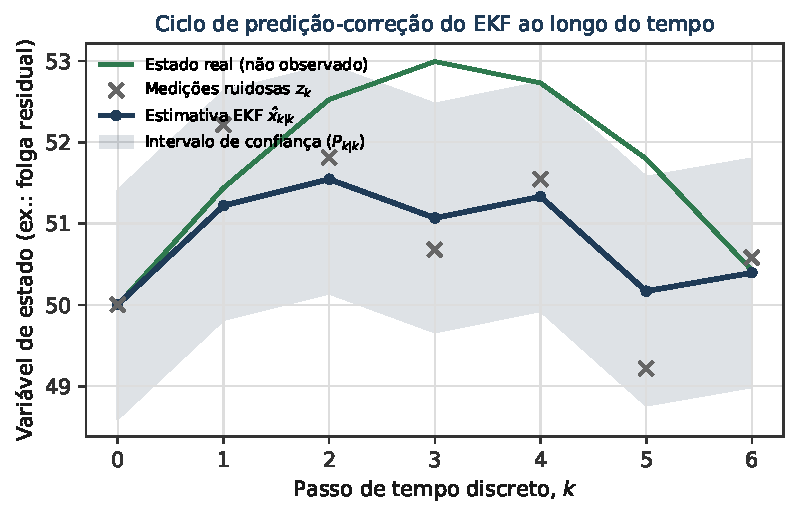
\includegraphics[width=0.60\textwidth]{figuras/fig_21_1_ekf.pdf}
		\caption[Ciclo de predição-correção do EKF]{Ciclo de predição-correção do EKF: estimativa convergindo para o estado real a partir de medições ruidosas, com banda de incerteza $P_{k|k}$.}
		\label{fig:21-1}
	\end{figure}

	\subsection{Condição de Observabilidade}

	O ciclo da Equação~\eqref{eq:s21-4} pode ser executado indefinidamente sem produzir nada de útil se o estado que se pretende estimar não deixar assinatura nas medições. Um estado \textbf{não observável} é aquele cujas variações não produzem efeito distinguível sobre $z$ — nesse caso o EKF não estima coisa alguma: ele apenas propaga a condição inicial com incerteza crescente, dando aparência de funcionamento enquanto o valor exibido no painel é ficção. Essa é a falha mais perigosa de um Gêmeo Digital, porque é silenciosa. Para o sistema linearizado a cada passo, a condição é a de posto completo da matriz de observabilidade $\mathcal{O}$, construída empilhando o Jacobiano de observação aplicado sucessivamente à dinâmica, conforme a Equação~\eqref{eq:s21-5}:

	\begin{equation}\label{eq:s21-5}
	\mathcal{O} = \begin{bmatrix} G_k \\ G_k F_k \\ G_k F_k^2 \\ \vdots \\ G_k F_k^{n_x-1} \end{bmatrix}, \qquad \text{observável} \iff \text{posto}(\mathcal{O}) = n_x
\end{equation}

	Onde $n_x$ é a dimensão do vetor de estado (cinco, no caso da Equação~\eqref{eq:s21-2}). O subscrito é necessário para não colidir com o índice politrópico $n$ dos capítulos de termodinâmica. Como $F_k$ e $G_k$ são recalculados a cada passo, a observabilidade no caso não linear é uma propriedade \textbf{local}, válida apenas na vizinhança do ponto de operação atual: um estado perfeitamente observável em plena carga pode deixar de sê-lo em carga reduzida, quando o efeito da folga $\delta$ sobre a corrente elétrica se torna pequeno demais para emergir do ruído de medição. Na prática, o Gêmeo Digital deve avaliar o número de condição de $\mathcal{O}$ em tempo de execução — mais informativo que o posto, que é uma resposta binária sobre uma matriz numérica — e sinalizar quando a estimativa de um estado específico deixou de ser sustentada pelos dados, em vez de continuar exibindo um número sem suporte na medição.

	\subsection{Inovação e Validação Estatística do Filtro}

	Existe uma grandeza que permite auditar a saúde do EKF em tempo real sem conhecer o estado verdadeiro: a \textbf{inovação}, definida como a diferença entre o que o sensor mediu e o que o modelo previa que ele mediria. Ela aparece dentro da própria etapa de correção da Equação~\eqref{eq:s21-4}, mas seu valor diagnóstico justifica tratá-la como grandeza de primeira classe, com sua covariância associada $S_k$, conforme a Equação~\eqref{eq:s21-6}:

	\begin{equation}\label{eq:s21-6}
	\tilde{z}_k = z_k - g(\hat{x}_{k|k-1}), \qquad S_k = G_k P_{k|k-1} G_k^T + \mathcal{R}
\end{equation}

	A teoria faz uma previsão forte e verificável sobre essa grandeza: se o modelo físico, as covariâncias $Q$ e $\mathcal{R}$ e as hipóteses de ruído estiverem corretos, a sequência de inovações deve ser um \textbf{ruído branco de média zero} com covariância exatamente $S_k$. Qualquer desvio desse comportamento é evidência de que alguma dessas premissas falhou. O teste padrão é a estatística NIS (\textit{Normalized Innovation Squared}), que normaliza a inovação pela incerteza esperada e cujo valor segue uma distribuição $\chi^2$ com tantos graus de liberdade quanto medições, conforme a Equação~\eqref{eq:s21-7}:

	\begin{equation}\label{eq:s21-7}
	\text{NIS}_k = \tilde{z}_k^T S_k^{-1} \tilde{z}_k \;\sim\; \chi^2_{n_z}
\end{equation}

	Onde $n_z$ é a dimensão do vetor de medições (também cinco aqui), grafada com subscrito para não colidir com o módulo de engrenagem $m$ do Capítulo 8. A interpretação operacional é direta e vale a pena explicitar, porque é ela que transforma uma identidade estatística em ferramenta de manutenção. Um NIS \textbf{consistentemente acima} da faixa esperada significa que o filtro está mais confiante do que deveria: as inovações são maiores do que $S_k$ prevê, indicando ou modelo físico defasado (a máquina degradou de um jeito que o modelo não captura) ou $Q$ subestimada. Um NIS \textbf{consistentemente abaixo} indica o contrário — covariâncias infladas, filtro excessivamente conservador, respondendo devagar demais a mudanças reais. E uma inovação com \textbf{média não nula} denuncia viés: tipicamente um sensor descalibrado ou um erro sistemático no modelo.

	Note que o NIS é calculável a cada passo sem qualquer conhecimento do estado verdadeiro. Isso o torna o único indicador realmente disponível em campo para responder à pergunta ``posso confiar nesta estimativa?'', e é a razão pela qual ele deve ser registrado e tendenciado junto com as próprias variáveis estimadas — um EKF sem monitoramento de inovação é um instrumento sem verificação de calibração.

	\subsection{Condicionamento Numérico: a Forma de Joseph}

	A atualização de covariância $P_{k|k} = (I - K_k G_k) P_{k|k-1}$, usada na Equação~\eqref{eq:s21-4} por ser a mais compacta, tem um defeito conhecido em implementações de precisão finita: ela não garante que $P$ permaneça simétrica e positiva definida. Erros de arredondamento acumulados ao longo de milhões de ciclos — e um Gêmeo Digital operando continuamente executa exatamente isso — podem tornar $P$ indefinida, momento em que o filtro diverge de forma abrupta e irrecuperável. A forma de Joseph, algebricamente equivalente mas numericamente estável por ser uma soma de dois termos estruturalmente positivos semidefinidos, é a implementação recomendada em produção, conforme a Equação~\eqref{eq:s21-8}:

	\begin{equation}\label{eq:s21-8}
	P_{k|k} = (I - K_k G_k) P_{k|k-1} (I - K_k G_k)^T + K_k \mathcal{R} K_k^T
\end{equation}

	O custo é um punhado de multiplicações matriciais adicionais por ciclo — irrelevante diante da taxa de amostragem de um compressor industrial, e barato demais para justificar o risco da forma simplificada.

	\subsection{Limites da Linearização e Alternativas}

	O EKF lineariza em torno da estimativa atual, o que embute uma hipótese: a de que a não linearidade do processo é suave o bastante para que o Jacobiano seja uma boa aproximação dentro da região de incerteza. Essa hipótese vale bem para os fenômenos térmicos e de eficiência tratados aqui, cujas curvas são monótonas e de curvatura moderada. Ela se degrada em dois cenários específicos deste equipamento: transientes rápidos de comutação das torres PSA, onde a dinâmica muda de regime em segundos, e a região próxima ao \textit{surge} ou ao travamento de válvula, onde o comportamento é fortemente não linear e a linearização local pode apontar na direção errada.

	Quando esses regimes forem relevantes para a aplicação, duas alternativas se impõem. O \textbf{Filtro de Kalman \textit{Unscented}} (UKF) substitui a linearização analítica pela propagação determinística de um conjunto de pontos amostrais (\textit{sigma points}) através da função não linear, capturando a média e a covariância com precisão de segunda ordem sem calcular Jacobianos — o que também elimina a necessidade de derivar $F_k$ e $G_k$ analiticamente, tarefa trabalhosa e propensa a erro num modelo com dezenas de acoplamentos. A \textbf{Estimação de Horizonte Móvel} (MHE), por sua vez, abandona a recursão de passo único e resolve, a cada instante, um problema de otimização sobre uma janela de medições passadas, o que permite impor \textbf{restrições explícitas} ao estado estimado — por exemplo, que a folga $\delta$ não pode ser negativa nem diminuir com o tempo, uma informação física que o EKF não tem como incorporar. Essa é precisamente a capacidade oferecida pelo \textit{framework} do-mpc discutido no Capítulo 27, e é o caminho natural de evolução deste módulo.

	\vspace{1em}
	\hrule
	\vspace{1em}

	\textbf{Diretriz Técnica Final:} O ciclo de predição-correção da Equação~\eqref{eq:s21-4} só produz estimativas confiáveis se três condições forem verificadas e monitoradas, não assumidas: observabilidade local do estado no ponto de operação corrente (Equação~\eqref{eq:s21-5}), consistência estatística da sequência de inovações via NIS (Equação~\eqref{eq:s21-7}) e estabilidade numérica da covariância via forma de Joseph (Equação~\eqref{eq:s21-8}). Matrizes $Q$ e $\mathcal{R}$ copiadas de outra instalação sem recalibração são a causa mais comum de um EKF que diverge ou passa a ignorar as medições — e o NIS é o instrumento que detecta isso antes que a estimativa errada chegue à decisão de manutenção.

	\clearpage
	\section{Redução de Dimensionalidade via Autoencoder Variacional (VAE)}
	
	A redução de dimensionalidade via VAE permite a compressão de dados complexos em assinaturas de saúde simplificadas, facilitando a detecção precoce de anomalias. A formulação usada aqui é a de Kingma e Welling \cite{vae}, que introduziu o autoencoder variacional como modelo generativo treinável por gradiente.

	\subsection{Por que um VAE, e não PCA ou um Autoencoder Simples}

	A pergunta antecede a matemática e merece resposta explícita, porque as três técnicas fazem redução de dimensionalidade e a escolha entre elas não é indiferente ao propósito de diagnóstico.

	A \textbf{Análise de Componentes Principais} (PCA) encontra a projeção linear que preserva o máximo de variância. É rápida, determinística e interpretável — mas linear. O acoplamento entre folga de rotor, temperatura de descarga e corrente elétrica neste equipamento é governado por relações politrópicas e exponenciais, mapeadas em detalhe na Parte I; forçá-las num subespaço linear descarta exatamente a estrutura que carrega a informação de degradação incipiente.

	O \textbf{autoencoder determinístico} resolve a não linearidade, mas produz um espaço latente sem estrutura garantida: nada impede que ele distribua os dados de treino arbitrariamente, com regiões vazias entre os aglomerados. Um ponto de operação novo, ainda saudável, pode cair numa dessas lacunas e gerar erro de reconstrução alto — um falso alarme.

	O \textbf{VAE} resolve os dois problemas ao impor que o espaço latente siga uma distribuição conhecida. Isso força a continuidade: pontos próximos no espaço latente decodificam para estados físicos próximos, sem lacunas arbitrárias. Para o diagnóstico, essa propriedade é o que permite interpretar a \textit{posição} no espaço latente — e não apenas o erro de reconstrução — como assinatura de saúde da máquina.
	
	\subsection{Arquitetura Probabilística e Espaço Latente}
	O VAE projeta o vetor de 28 variáveis em um espaço latente ($\ell$) modelado por distribuições gaussianas. A Figura~\ref{fig:22-1} ilustra essa arquitetura de ``gargalo'': o encoder comprime progressivamente a entrada $z$ até os poucos parâmetros do espaço latente, e o decoder expande esse gargalo de volta ao tamanho original, produzindo a reconstrução $\hat{z}$ — a diferença entre $z$ e $\hat{z}$ é justamente o erro de reconstrução usado como resíduo de diagnóstico mais adiante neste capítulo.

	\begin{figure}[h!tbp]
		\centering
		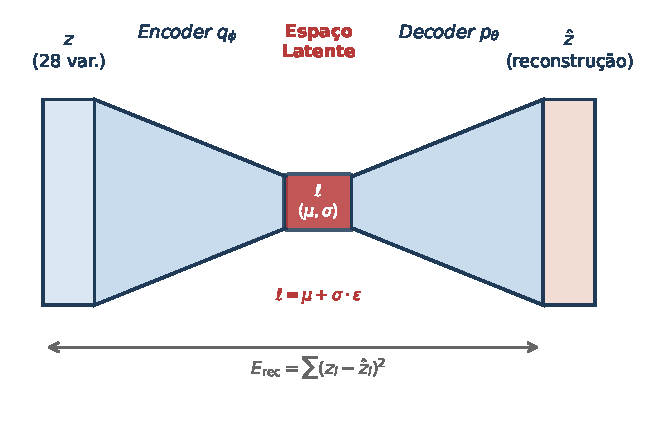
\includegraphics[width=0.75\textwidth]{figuras/fig_22_1_vae.pdf}
		\caption[Arquitetura do Autoencoder Variacional]{Arquitetura do Autoencoder Variacional: o encoder comprime o vetor de entrada $z$ até o espaço latente $\ell$ (parametrizado por $\mu$ e $\sigma$), e o decoder reconstrói $\hat{z}$ a partir dele.}
		\label{fig:22-1}
	\end{figure}

	\begin{itemize}
		\item \textbf{Encoder:} Mapeia a entrada $z$ para os parâmetros $\mu$ (média) e $\sigma$ (desvio padrão).
		\item \textbf{Reparametrização:} Para permitir a retropropagação do gradiente através de uma amostragem estocástica, o vetor latente é obtido deslocando a média por um ruído gaussiano padrão escalado pelo desvio padrão aprendido, conforme a Equação~\eqref{eq:s22-1}:
		\begin{equation}\label{eq:s22-1}
 \ell = \mu + \sigma \cdotp \epsilon, \quad \epsilon \sim \mathcal{N}(0,1)
\end{equation}
	\end{itemize}

	\subsection{Origem da Função de Perda: o Limite Inferior da Evidência}

	A função de perda do VAE não é uma combinação heurística de dois termos convenientes — ela é consequência direta de um problema de inferência bem posto, e entender essa origem é o que permite ajustá-la com critério em vez de por tentativa e erro.

	O objetivo ideal seria maximizar a verossimilhança dos dados observados, $\log p(z)$: encontrar os parâmetros de rede que tornam os dados de operação saudável os mais prováveis possíveis. O problema é que calcular $p(z)$ exige integrar sobre todas as configurações possíveis do espaço latente, uma integral intratável. A saída é introduzir uma distribuição aproximada $q(\ell|z)$ — justamente o que o encoder produz — e maximizar, em vez da verossimilhança, um limite inferior a ela. Esse limite é o ELBO (\textit{Evidence Lower Bound}), estabelecido por Kingma e Welling como objetivo diretamente treinável por gradiente \cite{vae} e formalizado na Equação~\eqref{eq:s22-2}:

	\begin{equation}\label{eq:s22-2}
	\log p(z) \;\ge\; \underbrace{\mathbb{E}_{q(\ell|z)}\left[ \log p(z|\ell) \right]}_{\text{verossimilhança da reconstrução}} \;-\; \underbrace{D_{KL}\left[ q(\ell|z) \parallel p(\ell) \right]}_{\text{afastamento da distribuição-alvo}}
\end{equation}

	Os dois termos do ELBO têm leitura direta. O primeiro pergunta: dado o código latente que o encoder gerou, quão provável é reconstruir a entrada original? Maximizá-lo é minimizar o erro de reconstrução. O segundo mede o quanto a distribuição produzida pelo encoder se afasta da distribuição-alvo $p(\ell) = \mathcal{N}(0,1)$; minimizá-lo é o que impõe a estrutura contínua no espaço latente discutida acima. Maximizar o ELBO é, portanto, exatamente equivalente a minimizar a perda da Equação~\eqref{eq:s22-3} — com o sinal trocado e com um peso $\beta$ acrescentado ao segundo termo.

	\subsection{Função de Perda e Regularização}
	Invertendo o sinal do ELBO e introduzindo o peso $\beta$, o treinamento busca o equilíbrio entre a fidelidade da reconstrução e a organização do espaço latente:
	\begin{equation}\label{eq:s22-3}
	L_{\text{VAE}} = \underbrace{\| z - \hat{z} \|^2}_{\text{Erro de Reconstrução}} + \beta \cdotp \underbrace{D_{KL} [ \mathcal{N}(\mu, \sigma) \parallel \mathcal{N}(0, 1) ]}_{\text{Divergência KL}}
\end{equation}

	O termo de divergência KL, que na forma geral exigiria integração numérica, admite \textbf{forma fechada} quando ambas as distribuições são gaussianas — que é precisamente o caso construído aqui. Essa é a razão prática de se escolher gaussianas: o gradiente sai analítico e o treinamento fica barato. Para um espaço latente de $d$ dimensões, a Equação~\eqref{eq:s22-4} dá a expressão implementada em código:

	\begin{equation}\label{eq:s22-4}
	D_{KL} = -\frac{1}{2} \sum_{j=1}^{d} \left( 1 + \log \sigma_j^2 - \mu_j^2 - \sigma_j^2 \right)
\end{equation}

	Vale notar o comportamento dessa expressão: ela se anula quando $\mu_j = 0$ e $\sigma_j = 1$ para toda dimensão $j$, e cresce conforme o encoder se afasta desse alvo. O parâmetro $\beta$ controla o quanto esse afastamento custa. Com $\beta \to 0$ o VAE degenera no autoencoder determinístico, com todas as patologias de espaço latente descritas anteriormente; com $\beta$ grande demais ocorre o \textit{posterior collapse}, em que o encoder passa a ignorar a entrada e emitir sempre $\mathcal{N}(0,1)$, produzindo reconstruções que são apenas a média dos dados de treino. Ambos os extremos destroem a capacidade de diagnóstico, e o sintoma do segundo é característico: erro de reconstrução alto e uniforme, insensível ao estado real da máquina.

	\subsection{Diagnóstico de Falhas por Resíduo}
	A saúde do sistema é monitorada pelo erro de reconstrução da Equação~\eqref{eq:s22-5}. Desvios em relação ao padrão aprendido indicam degradação mecânica ou térmica:
	\begin{equation}\label{eq:s22-5}
 E_{\text{rec}} = \sum_{i=1}^{M} (z_i - \hat{z}_i)^2
\end{equation}

	\subsection{A Premissa Crítica: Pureza do Conjunto de Treinamento}

	Toda a lógica de diagnóstico acima repousa numa premissa que raramente é enunciada e frequentemente é violada: o VAE deve ser treinado \textbf{exclusivamente com dados de operação saudável}. O erro de reconstrução só funciona como indicador de anomalia porque a rede nunca aprendeu a reconstruir estados degradados — confrontada com um, ela erra, e é esse erro que denuncia a falha.

	A consequência prática é severa. Se o histórico usado no treinamento contiver períodos em que a máquina já operava com mancal degradado ou trocador incrustado, a rede aprenderá esses estados como normais e passará a reconstruí-los com erro baixo. O Gêmeo Digital ficará então estruturalmente cego justamente à falha que mais ocorreu na planta. Como raramente existe garantia de que um histórico longo seja inteiramente saudável, a curadoria do conjunto de treinamento não é etapa preliminar dispensável, e sim requisito de projeto: os períodos devem ser filtrados contra registros de manutenção, e é recomendável usar o \textit{Isolation Forest} do Capítulo 25 como triagem prévia para remover do conjunto de treino os trechos anômalos antes de treinar o VAE.

	\subsection{Definição do Limiar de Disparo}

	O erro de reconstrução da Equação~\eqref{eq:s22-5} é um número sem escala absoluta — não existe valor universal de $E_{\text{rec}}$ que signifique ``falha''. O limiar $\tau_{\text{limiar}}$ precisa ser derivado da distribuição empírica do próprio erro sobre dados saudáveis não usados no treinamento (conjunto de validação), tomando um quantil elevado como corte, conforme a Equação~\eqref{eq:s22-6}:

	\begin{equation}\label{eq:s22-6}
	\tau_{\text{limiar}} = \mathcal{Q}_{1-\alpha}\left( \{ E_{\text{rec}}^{(i)} \}_{i \in \text{validação}} \right)
\end{equation}

	Onde $\mathcal{Q}_{1-\alpha}$ é o quantil de ordem $1-\alpha$ e $\alpha$ é a taxa de falsos alarmes aceita por projeto. A escolha de $\alpha$ é uma decisão de engenharia, não estatística: $\alpha = 0{,}01$ significa aceitar que aproximadamente um a cada cem pontos saudáveis dispare alarme. Numa planta offshore com aquisição a cada segundo, isso equivale a centenas de falsos alarmes por dia — inaceitável. Por isso o disparo deve exigir \textbf{persistência}, isto é, ultrapassagem de $\tau_{\text{limiar}}$ sustentada por uma janela temporal mínima, e não um único ponto isolado.

	\subsection{O Espaço Latente como Assinatura de Saúde}

	O erro de reconstrução responde \textit{se} algo está errado, mas não \textit{o quê}. A posição no espaço latente responde à segunda pergunta, e é aqui que a estrutura contínua imposta pela divergência KL rende seu segundo dividendo. Como modos de falha distintos deslocam a máquina para regiões diferentes do espaço latente, a distância de Mahalanobis entre o código latente atual e a distribuição dos códigos saudáveis fornece um indicador direcional, conforme a Equação~\eqref{eq:s22-7}:

	\begin{equation}\label{eq:s22-7}
	d_M(\ell) = \sqrt{ (\ell - \bar{\ell}_{\text{sadio}})^T \Sigma_{\text{sadio}}^{-1} (\ell - \bar{\ell}_{\text{sadio}}) }
\end{equation}

	Onde $\bar{\ell}_{\text{sadio}}$ e $\Sigma_{\text{sadio}}$ são a média e a covariância dos códigos latentes do conjunto saudável. A utilidade operacional é que, acumulando histórico, as regiões do espaço latente podem ser \textbf{rotuladas} com os modos de falha efetivamente observados na planta — transformando o VAE de detector genérico de anomalia em classificador de causa raiz, alimentado pela mesma matriz de mecanismos de falha construída na Parte I.

	\vspace{1em}
	\hrule
	\vspace{1em}

	\textbf{Diretriz Técnica Final:} O peso $\beta$ na Equação~\eqref{eq:s22-3} controla diretamente a sensibilidade do resíduo da Equação~\eqref{eq:s22-5}: um $\beta$ alto demais organiza o espaço latente às custas da fidelidade de reconstrução, mascarando desvios reais, até o limite do \textit{posterior collapse}; um $\beta$ baixo demais devolve as patologias do autoencoder determinístico. Antes disso, porém, vale a premissa que nenhuma sintonia corrige: um VAE treinado sobre histórico contaminado com operação degradada aprende a falha como normal e fica cego a ela. Curadoria do conjunto de treinamento primeiro, sintonia de $\beta$ depois, e limiar $\tau_{\text{limiar}}$ derivado por quantil da Equação~\eqref{eq:s22-6} com exigência de persistência — nunca um valor absoluto herdado de outra instalação.

	\clearpage
	\section{Aprendizado Informado pela Física (PIML)}

	O aprendizado informado pela física garante que a inteligência artificial opere estritamente dentro dos limites impostos pelas leis termodinâmicas e mecânicas. A formulação de redes neurais informadas pela física (PINNs), que fundamenta o PIML aqui aplicado, foi sistematizada por Raissi, Perdikaris e Karniadakis em 2019 como forma de incorporar equações diferenciais diretamente na função de perda de redes neurais \cite{piml}, e consolidada como campo de pesquisa na revisão abrangente de Karniadakis e colaboradores \cite{piml2}.
	
	\subsection{Integração de Restrições Físicas}
	A rede neural é treinada para minimizar o erro dos dados enquanto satisfaz o resíduo físico $\mathcal{F}$ (mesma notação usada no Capítulo de Fundamentos Teóricos; evita-se $\mathcal{R}$ aqui para não colidir com a covariância de ruído de medição do EKF) derivado de equações diferenciais. A construção é a proposta original de Raissi, Perdikaris e Karniadakis \cite{piml}: escrever a equação diferencial governante na forma de um resíduo que deve se anular e avaliá-lo sobre a própria saída da rede, transformando a lei física em uma parcela da função de perda. A Equação~\eqref{eq:s23-1} dá essa forma genérica:
	\begin{equation}\label{eq:s23-1}
 \mathcal{F} = \frac{\partial \hat{y}}{\partial t} + \mathcal{N}_{\text{phys}}[\hat{y}] = 0
\end{equation}

	\subsection{O Operador Físico Concreto deste Compressor}

	A Equação~\eqref{eq:s23-1} é um esqueleto: o operador $\mathcal{N}_{\text{phys}}$ é abstrato até que se diga quais leis, especificamente, a rede é obrigada a respeitar. Neste documento essa resposta já existe — ela é o conteúdo inteiro da Parte I. O PIML não introduz física nova; ele apenas transporta a física já equacionada componente a componente para dentro da função de perda da rede. A Equação~\eqref{eq:s23-2} explicita os três resíduos efetivamente impostos ao modelo do trem de compressão:

	\begin{equation}\label{eq:s23-2}
	\mathcal{F} = \begin{cases}
		\mathcal{F}_1 = \dot{m}_{\text{in}} - \dot{m}_{\text{out}} - \dfrac{dm_{\text{cv}}}{dt} & \text{(conservação de massa)} \\[10pt]
		\mathcal{F}_2 = \dot{W}_{\text{elec}}\,\eta_{\text{mot}} - \dot{m}\,\Delta h - \dot{Q}_{\text{rej}} - \dfrac{dU_{\text{cv}}}{dt} & \text{(conservação de energia)} \\[10pt]
		\mathcal{F}_3 = \max\left(0,\; -\dot{S}_{gen}\right) & \text{(Segunda Lei)}
	\end{cases}
\end{equation}

	Os dois primeiros resíduos são igualdades: a rede é penalizada proporcionalmente ao quanto sua predição desequilibra o balanço de massa ou de energia do volume de controle. O terceiro é de natureza diferente e merece atenção — é uma \textbf{desigualdade}, imposta pelo operador $\max$, que só penaliza quando a taxa de geração de entropia predita é negativa. Uma rede puramente orientada a dados pode perfeitamente prever, por interpolação entre pontos de treino, uma combinação de temperaturas e pressões que corresponderia a um processo de entropia decrescente — termodinamicamente impossível, mas numericamente plausível para um interpolador. O resíduo $\mathcal{F}_3$ é a barreira que impede essa predição de sobreviver ao treinamento, e é o exemplo mais nítido de por que a Parte I precisou vir antes da Parte II.

	\subsection{Função de Perda Híbrida}
	A função de custo soma o erro nos dados observados à violação dos resíduos da Equação~\eqref{eq:s23-2}, penalizando predições que contrariem a conservação de massa, a conservação de energia ou a Segunda Lei. Essa soma de duas parcelas ponderadas — um termo supervisionado sobre pontos medidos e um termo de resíduo sobre pontos de colocação — é a forma canônica da perda de uma PINN \cite{piml}, formalizada na Equação~\eqref{eq:s23-3}, e é o que a distingue de uma rede convencional treinada apenas em dados:
	\begin{equation}\label{eq:s23-3}
 L_{\text{PIML}} = \frac{1}{N} \sum (y - \hat{y})^2 + \lambda \cdotp \frac{1}{N_f} \sum \| \mathcal{F}(\hat{y}) \|^2
\end{equation}
	Onde $\lambda$ é o peso da consistência física no aprendizado, $N$ o número de pontos de dados medidos e $N_f$ o número de pontos de colocação, definidos a seguir.

	\subsection{Pontos de Colocação e Diferenciação Automática}

	Dois detalhes de implementação distinguem uma PINN de uma rede convencional, e ambos costumam ser omitidos em descrições de alto nível — o que leva à impressão equivocada de que basta ``somar um termo físico'' à perda.

	O primeiro é como as derivadas de $\mathcal{F}$ são obtidas. Elas não são calculadas por diferenças finitas sobre uma malha, como num solver numérico clássico; são obtidas por \textbf{diferenciação automática}, o mesmo mecanismo que a biblioteca já usa para propagar gradientes no treinamento. Como a rede é uma composição de funções analíticas, $\partial \hat{y} / \partial t$ é exata até precisão de máquina, sem erro de truncamento e sem necessidade de discretizar o domínio. É essa propriedade que torna a abordagem viável.

	O segundo é onde o resíduo físico é avaliado. Os \textbf{pontos de colocação} — os $N_f$ pontos do segundo somatório da Equação~\eqref{eq:s23-3} — são posições no domínio de entrada onde se exige que a física seja satisfeita, e são \textbf{independentes dos dados medidos}. Eles não precisam de sensor algum, apenas de coordenadas. A consequência é o que dá ao PIML sua vantagem decisiva neste projeto: é possível impor conservação de energia em regiões do envelope operacional onde \textbf{nunca houve medição} — em razões de pressão que a máquina raramente atinge, em temperaturas ambientes extremas. Uma rede puramente orientada a dados extrapola nessas regiões sem qualquer garantia; a PINN ao menos extrapola sem violar as leis de conservação. Para um equipamento offshore, onde o custo de levar a máquina a condições extremas para coletar dados é proibitivo, essa é a diferença entre um modelo utilizável e um modelo restrito ao ponto de operação nominal.

	\subsection{Balanceamento Adaptativo dos Termos de Perda}

	O peso $\lambda$ fixo da Equação~\eqref{eq:s23-3} esconde um problema numérico real: os dois termos da perda têm escalas físicas completamente diferentes. Um resíduo de conservação de energia expresso em watts e um erro de temperatura expresso em kelvin diferem em ordens de grandeza, e o gradiente do termo maior domina o treinamento, tornando o outro efetivamente invisível ao otimizador. Sintonizar $\lambda$ manualmente contra esse desbalanço é trabalhoso e frágil.

	A alternativa recomendada é ajustar o peso ao longo do treinamento, em função da magnitude relativa dos gradientes de cada termo, conforme a Equação~\eqref{eq:s23-4}:

	\begin{equation}\label{eq:s23-4}
	\lambda^{(t+1)} = (1-\kappa)\,\lambda^{(t)} + \kappa \cdot \frac{\overline{\left| \nabla_\theta L_{\text{dados}} \right|}}{\overline{\left| \nabla_\theta L_{\text{física}} \right|}}
\end{equation}

	Onde $\theta$ são os parâmetros da rede, as barras indicam a média das magnitudes dos gradientes na iteração corrente e $\kappa \in (0,1)$ é um fator de suavização que evita oscilação brusca do peso. O efeito é equalizar automaticamente a influência dos dois termos sobre o passo de otimização, independentemente das unidades em que cada um foi escrito. Além disso, quando os três resíduos da Equação~\eqref{eq:s23-2} têm escalas muito distintas entre si, a prática correta é atribuir um peso próprio a cada um, em vez de um $\lambda$ único para o bloco físico inteiro.

	\subsection{Limitações e Cautelas}

	A revisão de Karniadakis e colaboradores \cite{piml2} — a mesma que consolidou o campo — é explícita quanto às suas limitações, e reproduzi-las aqui é mais honesto do que apresentar o PIML como garantia automática de validade física.

	Primeiro, e mais importante: a penalização é \textbf{fraca}, não uma restrição rígida. Minimizar $\| \mathcal{F} \|^2$ reduz a violação das leis físicas, mas não a zera. A rede treinada produz predições \textit{aproximadamente} conservativas, e a magnitude residual dessa violação precisa ser medida e reportada, não presumida desprezível. Onde a garantia precisar ser dura — numa restrição de segurança, por exemplo — a imposição deve ser feita na camada de otimização com restrições do MPC (Capítulo 24), não na perda da rede.

	Segundo, o treinamento de PINNs é notoriamente mais difícil de convergir que o de redes convencionais. O panorama de otimização é mal condicionado, e patologias de gradiente entre os termos são frequentes — daí a necessidade do balanceamento adaptativo descrito acima.

	Terceiro, o benchmarking do campo ainda é imaturo: comparações justas entre PINNs e solvers numéricos clássicos são escassas, e para problemas em que já existe um solver rápido e confiável, a PINN pode não oferecer vantagem alguma. Neste projeto a justificativa é específica e deve ser mantida à vista: substituir simulações CFD caras por um modelo substituto (\textit{surrogate}) que responde em milissegundos, viabilizando o uso em laço de controle — e não superar o CFD em acurácia.

	\subsection{Divisão de Papéis entre PIML e EKF}

	Uma dúvida legítima surge neste ponto: se o EKF do Capítulo 21 também usa o modelo físico, e o PIML também estima grandezas não medidas, os dois não estariam fazendo a mesma coisa? Não — e a distinção esclarece a arquitetura do Gêmeo Digital.

	O EKF opera \textbf{online}, num único ponto no tempo, e responde: ``dado o modelo físico e a medição que acabou de chegar, qual o estado mais provável agora?''. Sua saída é uma estimativa com incerteza quantificada, atualizada a cada ciclo de varredura. O PIML opera \textbf{offline}, sobre todo o histórico, e responde: ``que função aproxima o comportamento desta máquina em todo o envelope operacional, inclusive onde não há dados, sem violar as leis de conservação?''. Sua saída é um modelo substituto rápido.

	Os dois se compõem em vez de competir: o modelo substituto treinado por PIML pode ser usado \textit{como} a função de transição $f(\cdot)$ do EKF, substituindo um modelo físico analítico caro de avaliar por uma rede que roda em microssegundos — o que permite ao EKF operar em taxa de amostragem alta o suficiente para capturar transientes rápidos. E o mesmo substituto serve de modelo de predição para o MPC do Capítulo 24, onde o custo de avaliação é multiplicado por todo o horizonte de otimização.

	\subsection{Identificação de Parâmetros por Problema Inverso}

	A formulação original de Raissi, Perdikaris e Karniadakis \cite{piml} cobre dois problemas com a mesma máquina matemática: o \textbf{problema direto} — conhecidos os parâmetros físicos, prever o estado — que é o que as subseções anteriores descreveram; e o \textbf{problema inverso} — conhecido o estado, a partir de medições de campo, identificar o parâmetro físico que o produziu. É a mesma pergunta que motiva a Seção~28.1 deste documento (calibração via EKF com estado aumentado), mas resolvida aqui por um mecanismo diferente, mais adequado quando o parâmetro procurado varia com a posição no domínio — não só com o tempo — ou quando não há necessidade de estimativa em tempo real, apenas uma calibração única a partir do histórico acumulado de operação.

	A diferença de formulação é pequena, mas decisiva. Em vez de tratar o parâmetro físico $\Xi$ (ex.: um coeficiente de perda, a condutância de um trocador, a rigidez de um elemento) como constante conhecida dentro do operador $\mathcal{N}_{\text{phys}}$ da Equação~\eqref{eq:s23-1}, ele passa a ser mais uma variável treinável da rede — otimizada junto com os pesos $\theta$, não fixada antes do treinamento, na Equação~\eqref{eq:s23-5}:

	\begin{equation}\label{eq:s23-5}
	\min_{\theta,\, \Xi} \; L_{\text{inv}}(\theta, \Xi) = \frac{1}{N}\sum (y-\hat{y})^2 + \lambda \cdot \frac{1}{N_f}\sum \left\| \mathcal{F}(\hat{y}; \Xi) \right\|^2
	\end{equation}

	A rede aprende simultaneamente a reproduzir os dados medidos e o valor de $\Xi$ que torna essa reprodução consistente com a física — exatamente o mecanismo que a Tabela~\ref{tab:27-1} atribui ao DeepXDE, ferramenta especializada em problemas inversos sobre equações diferenciais, na camada de \textit{PDE Solver} da arquitetura de alta performance do Capítulo 27.

	Essa técnica responde a uma limitação real deste documento: os parâmetros de catálogo usados na Parte I são valores de referência de fabricante, calibrados em condições padronizadas de bancada, e podem variar de forma sistemática de uma instalação real para outra — por qualidade de montagem, tipo de invólucro (Capítulo 2), condições ambientais do sítio ou o lote de fabricação do componente. Um problema inverso resolvido sobre o histórico de operação de \textbf{cada} unidade instalada devolve o valor efetivo daquele parâmetro \textit{para aquele local e aquele tipo de instalação específicos}, em vez de herdar cegamente o valor de catálogo — o mesmo objetivo da Seção~28.1, por um caminho offline e capaz de lidar com parâmetros distribuídos no espaço, não só no tempo.

	\vspace{1em}
	\hrule
	\vspace{1em}

	\textbf{Diretriz Técnica Final:} O peso $\lambda$ na Equação~\eqref{eq:s23-3} deve ser balanceado pela magnitude relativa dos gradientes (Equação~\eqref{eq:s23-4}), não fixado arbitrariamente — $\lambda$ excessivo faz a rede ignorar os dados reais em favor da física idealizada, enquanto $\lambda$ insuficiente permite predições que violam conservação de massa/energia mesmo com baixo erro nos dados de treino. Igualmente importante: a penalização física é fraca, não uma garantia. O resíduo $\| \mathcal{F} \|$ da rede treinada deve ser medido e reportado como métrica de aceitação, e nenhuma restrição de segurança do equipamento deve depender exclusivamente dela — restrições duras pertencem à camada de otimização com restrições do Capítulo 24. A identificação por problema inverso (Equação~\eqref{eq:s23-5}) herda a mesma cautela: um parâmetro $\Xi$ identificado offline deve ser validado contra a faixa plausível de catálogo antes de substituir o valor de referência em produção, pelo mesmo motivo que a Seção~28.2 exige análise de sensibilidade para parâmetros da categoria (iv).

	\clearpage
	\section{Otimização e Controle: MPC e PSO}
	
	A camada de decisão e otimização utiliza algoritmos preditivos e heurísticos para maximizar a eficiência exergética e a vida útil dos componentes.
	
	\subsection{Controle Preditivo Baseado em Modelo (MPC)}
	O MPC, consolidado como referência de controle de processos industriais por Camacho e Bordons \cite{mpc} e formalizado em teoria, computação e projeto por Rawlings, Mayne e Diehl \cite{rawlings}, projeta o comportamento do sistema em um horizonte $H$ para otimizar as variáveis de controle ($u$). A Figura~\ref{fig:24-1} ilustra o princípio de horizonte deslizante (\textit{receding horizon}) que dá nome ao método: a cada instante $k$, o controlador usa o modelo físico para projetar a trajetória futura de $y$ ao longo de todo o horizonte $H$, otimiza toda a sequência de ações de controle, mas aplica apenas a primeira ($u(k)$) — no instante seguinte, com uma nova medição disponível, todo o processo se repete com o horizonte deslocado um passo à frente:

	\begin{figure}[h!tbp]
		\centering
		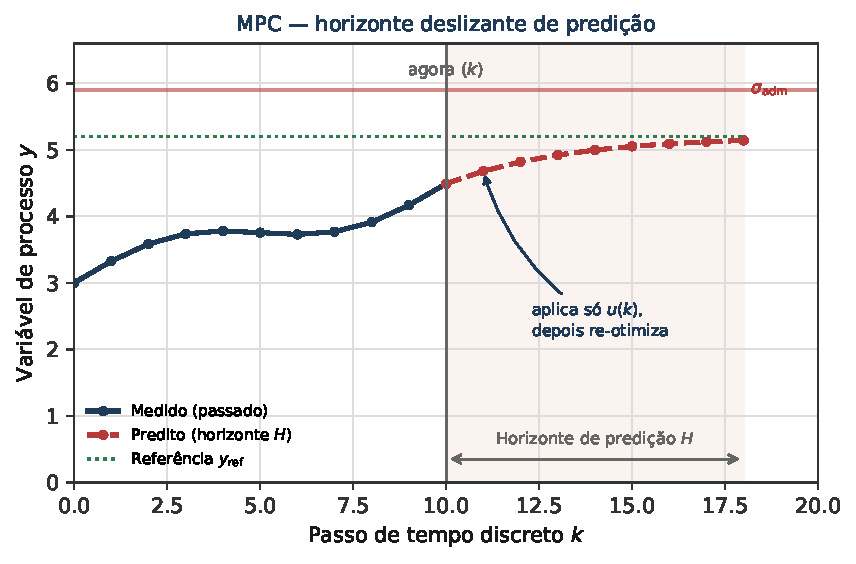
\includegraphics[width=0.60\textwidth]{figuras/fig_24_1_mpc.pdf}
		\caption[Princípio de horizonte deslizante do MPC]{Princípio de horizonte deslizante do MPC: a trajetória prevista (tracejada) é otimizada até o fim do horizonte $H$, mas só a primeira ação de controle é aplicada antes de reotimizar.}
		\label{fig:24-1}
	\end{figure}

	A Equação~\eqref{eq:s24-1} formaliza esse princípio na formulação quadrática padrão do MPC \cite[Cap.~2]{rawlings}: um primeiro somatório penalizando o desvio quadrático da saída em relação à referência ao longo de todo o horizonte, e um segundo penalizando o esforço de controle — ambos sujeitos ao modelo de predição do processo e às restrições de integridade mecânica. A escolha do quadrado não é estética: é ela que torna o problema convexo no caso linear e, portanto, resolúvel de forma confiável dentro do período de amostragem do controlador.

	\begin{equation}\label{eq:s24-1}
	\begin{aligned}
		\text{Minimizar } J &= \sum_{k=1}^{H} [ y(k) - y_{\text{ref}}(k) ]^2 + \rho \sum_{k=0}^{H-1} [ \Delta u(k) ]^2 \\[4pt]
		\text{Sujeito a: } & x_{k+1} = f(x_k, u_k) \\
		& \sigma_b(k) \le \sigma_{\text{adm}}
	\end{aligned}
\end{equation}
	É essa reotimização a cada passo — e não um cálculo único offline — que permite ao MPC reagir a distúrbios reais (uma flutuação de demanda, um desvio de temperatura) sem violar a restrição estrutural $\sigma_b(k) \le \sigma_{\text{adm}}$ em nenhum ponto do horizonte projetado.

	\subsubsection*{Sintonia do horizonte e do peso de esforço}

	Os dois parâmetros livres da Equação~\eqref{eq:s24-1} governam o comportamento do controlador, e ambos têm interpretação física direta neste equipamento.

	O horizonte $H$ deve cobrir a \textbf{dinâmica mais lenta} que o controlador precisa antecipar. Num sistema de ar comprimido, a constante de tempo dominante não é a do compressor, e sim a do vaso pulmão: a Equação~\eqref{eq:s3-5} descreve a dinâmica de pressão desse volume, e é ela que dita quanto tempo o sistema leva para responder a uma mudança de carga. Um horizonte curto demais faz o MPC agir como um PID míope, reagindo à pressão atual sem antecipar o esvaziamento do pulmão; um horizonte longo demais multiplica o custo computacional sem ganho, porque a incerteza da predição cresce e as ações do fim do horizonte são descartadas de qualquer modo. A regra prática é dimensionar $H$ para algo entre uma e duas constantes de tempo do vaso.

	O peso $\rho$ penaliza a \textbf{variação} da ação de controle, $\Delta u$, e não seu valor absoluto — distinção essencial. É ele que impede o controlador de perseguir cada flutuação de pressão com mudanças bruscas de frequência do VSD. Um $\rho$ baixo demais produz ciclagem do inversor: o controlador tecnicamente minimiza o erro, mas ao custo de fadiga térmica no motor e desgaste acelerado, degradando exatamente os componentes cuja vida útil o Gêmeo Digital deveria preservar. Trata-se, portanto, de um parâmetro que acopla o desempenho de controle à integridade mecânica, e sua sintonia deve considerar as duas coisas.

	\subsubsection*{Viabilidade e amolecimento de restrições}

	Há uma falha de projeto que derruba controladores MPC em campo e raramente aparece na formulação teórica: a \textbf{inviabilidade}. Se um distúrbio levar a máquina a um estado a partir do qual nenhuma sequência de ações satisfaz todas as restrições dentro do horizonte, o otimizador não retorna uma solução ruim — ele não retorna solução alguma. O controlador fica sem saída a aplicar, exatamente no momento de maior estresse do sistema.

	A proteção padrão é distinguir restrições \textbf{duras}, que jamais podem ser relaxadas, de restrições \textbf{brandas}, que podem ser violadas temporariamente a um custo alto. Isso se implementa com variáveis de folga $\varsigma \ge 0$ penalizadas na função objetivo, conforme a Equação~\eqref{eq:s24-2}:

	\begin{equation}\label{eq:s24-2}
	\begin{aligned}
		\text{Minimizar } J' &= J + \varrho_s \sum_{k=1}^{H} \varsigma_k^2 \\[4pt]
		\text{Sujeito a: } & \sigma_b(k) \le \sigma_{\text{adm}} && \text{(dura — integridade mecânica)} \\
		& T_{\text{dp}}(k) \le T_{\text{dp,set}} + \varsigma_k && \text{(branda — qualidade do ar)} \\
		& \varsigma_k \ge 0
	\end{aligned}
\end{equation}

	Onde $\varrho_s$ é uma penalidade deliberadamente alta, escolhida de modo que o otimizador só recorra à folga quando não houver alternativa viável. A classificação de cada restrição é uma decisão de engenharia com consequência de segurança, e deve ser explícita: a tensão na raiz do dente é \textbf{dura} porque sua violação é ruptura mecânica, irreversível; o ponto de orvalho é \textbf{brando} porque uma excursão de alguns minutos acima do setpoint durante um transiente de demanda degrada a qualidade do ar temporariamente, sem dano permanente ao equipamento. Confundir as duas categorias — endurecendo tudo — é a receita para um controlador que trava justamente quando é mais necessário.

	\subsubsection*{Modelo de predição e custo computacional}

	A restrição $x_{k+1} = f(x_k, u_k)$ da Equação~\eqref{eq:s24-1} exige avaliar o modelo físico uma vez por passo do horizonte, a cada iteração do otimizador, a cada ciclo de controle — o produto desses três fatores é o que determina a viabilidade em tempo real. Avaliar diretamente o equacionamento completo da Parte I, com suas correlações de troca térmica e psicrometria, é caro demais para essa multiplicação. É precisamente aqui que o modelo substituto treinado por PIML (Capítulo 23) deixa de ser refinamento acadêmico e vira requisito de arquitetura: ele fornece o mesmo $f(\cdot)$ com custo de avaliação ordens de grandeza menor, mantendo consistência física garantida por construção. A alternativa clássica — linearizar o modelo em torno do ponto de operação e resolver um problema quadrático — é mais barata ainda, mas perde validade justamente nos transientes amplos em que o MPC seria mais útil.

	\subsection{Otimização por Enxame de Partículas (PSO)}
	Introduzido por Kennedy e Eberhart em 1995 como metaheurística inspirada no comportamento social de bandos e cardumes \cite{pso}, o PSO é usado aqui para a sintonização de setpoints globais em superfícies de custo não convexas, utilizando a dinâmica de partículas da Equação~\eqref{eq:s24-3}:
	\begin{equation}\label{eq:s24-3}
 v_{i}^{t+1} = w v_{i}^t + c_1 r_1 (p_{\text{best},i} - x_{i}^t) + c_2 r_2 (g_{\text{best}} - x_{i}^t)
\end{equation}
	A Equação~\eqref{eq:s24-3} atualiza apenas a \textbf{velocidade} de cada partícula; o deslocamento propriamente dito vem da Equação~\eqref{eq:s24-4}, que completa a iteração do algoritmo:

	\begin{equation}\label{eq:s24-4}
	x_i^{t+1} = x_i^t + v_i^{t+1}
\end{equation}

	Os termos das duas equações têm leitura direta:
	\begin{itemize}
		\item $p_{\text{best},i}$: Melhor posição já visitada pela partícula $i$ (memória individual).
		\item $g_{\text{best}}$: Melhor posição já encontrada por todo o enxame (memória coletiva).
		\item $w$: Peso de inércia — controla quanto da velocidade anterior é conservado.
		\item $c_1, c_2$: Coeficientes cognitivo e social, que ponderam a atração pela melhor posição própria e pela melhor do grupo.
		\item $r_1, r_2 \sim \mathcal{U}(0,1)$: Números aleatórios sorteados a cada iteração, que introduzem a estocasticidade responsável pela exploração do espaço de busca.
	\end{itemize}

	\subsubsection*{Sintonia dos coeficientes e critério de parada}

	O peso de inércia $w$ governa o compromisso entre exploração e refinamento, e a prática consolidada é não mantê-lo fixo: iniciar alto (tipicamente próximo de $0{,}9$), favorecendo a varredura ampla do espaço de busca, e decair linearmente até um valor baixo (próximo de $0{,}4$) ao longo das iterações, concentrando o enxame em torno da melhor região encontrada. Um $w$ alto demais em regime permanente impede a convergência — as partículas orbitam o ótimo sem se assentar; um $w$ baixo desde o início faz o enxame colapsar prematuramente no primeiro mínimo local que encontrar, anulando a própria razão de se usar uma metaheurística em lugar de um método de gradiente.

	Os coeficientes $c_1$ e $c_2$ são comumente fixados em torno de $2{,}0$ cada. O desbalanço entre eles tem efeito previsível: $c_2 \gg c_1$ acelera a convergência ao custo de perda de diversidade, com o enxame inteiro perseguindo um único ponto e ficando vulnerável a mínimos locais; $c_1 \gg c_2$ produz o oposto, um enxame disperso que explora bem mas converge devagar.

	O critério de parada não deve ser apenas um número máximo de iterações. Duas condições adicionais são mais informativas: \textbf{estagnação} de $g_{\text{best}}$, isto é, ausência de melhoria relativa significativa por um número consecutivo de iterações, e \textbf{colapso de diversidade}, medido pela dispersão das posições das partículas. Este segundo critério merece destaque porque distingue duas situações que o primeiro confunde: um enxame que parou de melhorar \textit{porque convergiu} e um que parou \textit{porque perdeu diversidade cedo demais} e ficou preso. Só o segundo caso justifica reiniciar a busca com nova semeadura.
	A Figura~\ref{fig:24-2} mostra esse comportamento em duas iterações de um enxame sobre uma superfície de custo hipotética: inicialmente as partículas estão espalhadas e suas velocidades (setas) combinam o puxão em direção à melhor posição já visitada por cada uma ($p_{\text{best}}$) com o puxão em direção à melhor posição já vista por todo o enxame ($g_{\text{best}}$); depois de algumas iterações, o enxame converge e se concentra ao redor do mínimo global encontrado.

	\begin{figure}[h!tbp]
		\centering
		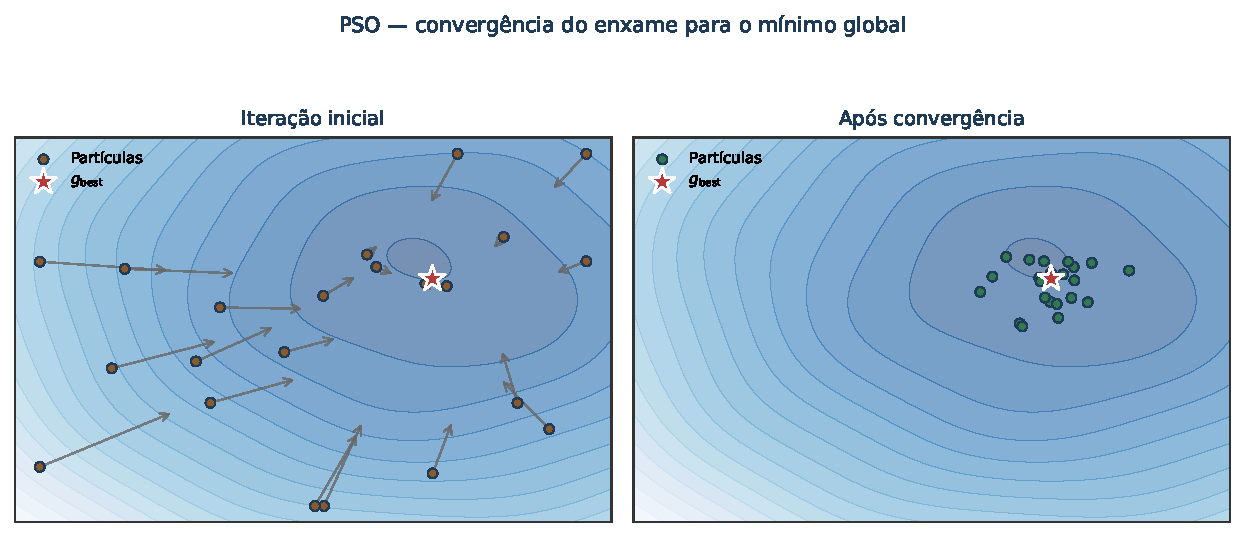
\includegraphics[width=0.75\textwidth]{figuras/fig_24_2_pso.pdf}
		\caption[Convergência do enxame de partículas do PSO]{Convergência do enxame de partículas do PSO sobre uma superfície de custo hipotética: dispersão inicial (esquerda) e concentração em torno do mínimo global $g_{\text{best}}$ após convergência (direita).}
		\label{fig:24-2}
	\end{figure}

	\vspace{1em}
	\hrule
	\vspace{1em}

	\textbf{Diretriz Técnica Final:} MPC e PSO cumprem papéis complementares, não intercambiáveis: o MPC (Equação~\eqref{eq:s24-1}) resolve o controle em tempo real dentro das restrições de integridade, enquanto o PSO é reservado para sintonia de hiperparâmetros e busca de setpoints globais offline — usar PSO no laço de controle em tempo real introduz latência incompatível com a proteção mecânica do compressor. Dois requisitos de projeto decorrem disso e não podem ser omitidos na implementação: o MPC precisa de tratamento explícito de inviabilidade, separando restrições duras de brandas com variáveis de folga (Equação~\eqref{eq:s24-2}), sob pena de o controlador não retornar ação alguma justamente durante o distúrbio que o exigia; e o modelo de predição $f(\cdot)$ deve ser barato o bastante para ser avaliado $H$ vezes por iteração do otimizador, o que na prática torna o substituto treinado por PIML (Capítulo 23) parte da arquitetura de controle, e não um acessório.

	\clearpage
	\section{Diretrizes para o Desenvolvimento e Evolução do Gêmeo Digital}
	
	Este capítulo apresenta recomendações técnicas essenciais para futuros desenvolvedores, focando na robustez, escalabilidade e confiabilidade do sistema em ambientes operacionais offshore.
	
	\subsection{Governança de Dados e Pré-processamento Robusto}
	O sucesso dos algoritmos de inferência, como o EKF e o VAE, depende criticamente da integridade dos sinais de entrada. Em ambientes offshore, a telemetria é frequentemente ruidosa.
	\begin{itemize}
		\item \textbf{Filtragem Adaptativa (Savitzky-Golay):} Diferente de uma média móvel simples — que suaviza o ruído mas também ``arredonda'' picos e mudanças bruscas reais do sinal —, o filtro de Savitzky-Golay \cite{savgol} ajusta um polinômio de grau $p_{\text{SG}}$ por mínimos quadrados dentro de uma janela móvel de $2m_{\text{SG}}+1$ amostras centrada em cada ponto, e usa o valor do polinômio ajustado no centro da janela como a amostra suavizada. Como esse ajuste é linear nos dados de entrada, o resultado se reduz a uma convolução com coeficientes fixos $c_i$ (pré-calculados uma única vez a partir de $p_{\text{SG}}$ e $m_{\text{SG}}$), Equação~\eqref{eq:s25-1}:
		\begin{equation}\label{eq:s25-1}
 y_j^{\text{suav}} = \sum_{i=-m_{\text{SG}}}^{m_{\text{SG}}} c_i \cdotp y_{j+i}
\end{equation}
		É justamente o ajuste polinomial local — em vez de uma média constante — que preserva a amplitude e a largura de transientes reais (como o pico de um impacto mecânico incipiente), ao mesmo tempo em que atenua o ruído de alta frequência da instrumentação; por isso o filtro é preferido à média móvel para os sinais de vibração deste documento.
		\item \textbf{Tratamento de Outliers (\textit{Isolation Forest}):} Ao contrário de métodos que primeiro modelam o que é ``normal'' para depois sinalizar desvios, o \textit{Isolation Forest} \cite{isoforest} explora diretamente a definição de anomalia — pontos raros e diferentes são mais fáceis de isolar. O algoritmo constrói um conjunto de árvores binárias aleatórias (\textit{isolation trees}), cada uma particionando os dados recursivamente por um atributo e um valor de corte escolhidos ao acaso; um ponto anômalo tende a ser isolado em poucas divisões (caminho curto até a raiz da árvore), enquanto um ponto normal exige muitas divisões (caminho longo). O escore de anomalia normaliza o comprimento médio do caminho de isolamento $E[L_{\text{iso}}(x)]$ sobre todas as árvores da floresta pelo comprimento médio esperado numa árvore de busca binária com $n_{\text{IF}}$ pontos, Equação~\eqref{eq:s25-2}:
		\begin{equation}\label{eq:s25-2}
 s_{\text{IF}}(x) = 2^{-\frac{E[L_{\text{iso}}(x)]}{c(n_{\text{IF}})}}, \quad c(n_{\text{IF}}) = 2\left[\ln(n_{\text{IF}}-1) + \gamma_{\text{EM}}\right] - \frac{2(n_{\text{IF}}-1)}{n_{\text{IF}}}
\end{equation}
		Onde $\gamma_{\text{EM}} \approx 0{,}5772$ é a constante de Euler-Mascheroni (subscrita para não colidir com a razão de calores específicos $\gamma$ usada nos capítulos de termodinâmica). Um escore $s_{\text{IF}}$ próximo de 1 indica forte probabilidade de anomalia (caminho de isolamento muito curto); próximo de 0,5, o ponto é indistinguível do comportamento normal. O Gêmeo Digital usa esse escore para filtrar picos espúrios de sensor antes que alimentem o EKF ou o VAE, evitando falsos diagnósticos de falha originados por ruído de instrumentação, não por degradação real do equipamento. A Figura~\ref{fig:25-1} ilustra a ideia geometricamente: um ponto anômalo isolado do resto dos dados é separado do restante em poucos cortes retangulares aleatórios, enquanto um ponto no meio do aglomerado normal só se isola depois de muitos cortes sucessivos.

		\begin{figure}[h!tbp]
			\centering
			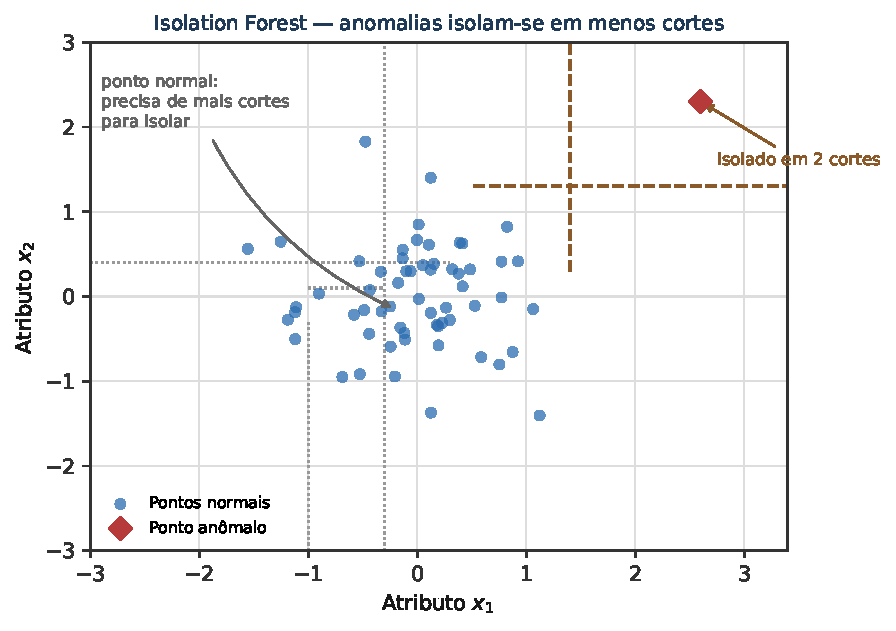
\includegraphics[width=0.60\textwidth]{figuras/fig_25_1_isoforest.pdf}
			\caption[Princípio do \textit{Isolation Forest}]{Princípio do \textit{Isolation Forest}: um ponto anômalo se isola do restante dos dados em poucos cortes aleatórios; um ponto no meio de um aglomerado normal exige muito mais cortes.}
			\label{fig:25-1}
		\end{figure}
	\end{itemize}
	
	\subsection{Quantificação de Incerteza (UQ)}
	Um Gêmeo Digital de missão crítica não deve fornecer apenas valores determinísticos, mas sim intervalos de confiança para suportar a tomada de decisão segura.
	\begin{itemize}
		\item \textbf{Propagação de Erro:} A incerteza dos sensores deve ser propagada para os KPIs globais, como a destruição de exergia ($\dot{I}$). A Equação~\eqref{eq:s25-3} é a fórmula clássica de propagação de incerteza: cada temperatura medida $T_i$ contribui para a incerteza total de $\dot{I}$ na proporção de quão sensível $\dot{I}$ é àquela temperatura específica (a derivada parcial) multiplicada pela incerteza do próprio sensor $u(T_i)$, somadas em quadratura:
		\begin{equation}\label{eq:s25-3}
 u(\dot{I}) = \sqrt{\sum_{i=1}^{n} \left( \frac{\partial \dot{I}}{\partial T_i} \right)^2 u(T_i)^2}
\end{equation}
		\item \textbf{Redes Bayesianas:} Substituição de camadas densas por camadas bayesianas no PIML para obter a variância da predição ($\sigma^2$).
	\end{itemize}
	
	\subsection{Arquitetura de Computação em Borda (Edge Computing)}
	Dada a latência de comunicação via satélite em plataformas, a arquitetura deve ser distribuída para garantir respostas em tempo real.
	\begin{itemize}
		\item \textbf{Processamento Local (Edge):} Algoritmos de alta frequência, como a análise de harmônicos de vibração e o EKF, devem ser executados próximos ao ativo físico.
		\item \textbf{Processamento em Nuvem (Cloud):} O treinamento de modelos pesados (VAE) e a otimização de longo prazo (MPC) devem ser centralizados para aproveitar maior capacidade computacional.
	\end{itemize}
	
	\subsection{Explicabilidade e Interface Humano-Máquina (XAI)}
	Para que o Gêmeo Digital seja aceito pelos operadores, suas decisões devem ser auditáveis e compreensíveis.
	\begin{itemize}
		\item \textbf{Valores de SHAP:} Utilização de \textit{SHapley Additive exPlanations} para quantificar a contribuição de cada sensor em um diagnóstico de falha. A Equação~\eqref{eq:s25-4}, originada da teoria de jogos cooperativos, calcula a contribuição média da variável $x_i$ ($\phi_i$) testando o modelo $f$ com e sem essa variável, em todas as combinações possíveis ($S$) das demais variáveis — o resultado é um ``crédito'' justo de quanto cada sensor pesou na decisão do modelo, permitindo ao operador ver, por exemplo, que um alarme foi disparado principalmente por $T_{dp}$ e não por vibração:
		\begin{equation}\label{eq:s25-4}
 \phi_i(f) = \sum_{S \subseteq \{x_1, \dots, x_n\} \setminus \{x_i\}} \frac{|S|! (n - |S| - 1)!}{n!} [f(S \cup \{x_i\}) - f(S)]
\end{equation}
		\item \textbf{Visualização Latente:} Projeção do espaço latente do VAE em duas dimensões para visualização intuitiva da trajetória de degradação do ativo.
	\end{itemize}
	
	\subsection{Ciclo de Vida e MLOps (Model Drift)}
	O ativo físico sofre modificações estruturais ao longo do tempo (substituição de componentes, novos selos). O modelo digital deve evoluir em sincronia com o físico.
	\begin{itemize}
		\item \textbf{Detecção de Drift:} Monitoramento contínuo do erro de reconstrução do VAE. Se o erro crescer consistentemente após uma manutenção, o modelo deve ser retreinado.
		\item \textbf{Pipeline de Retreinamento:} Automação do fluxo de coleta de dados históricos para ajuste dos pesos sinápticos ($\theta, \phi$) do modelo híbrido.
	\end{itemize}
	
	\vspace{1em}
	\hrule
	\vspace{1em}
	
	\textbf{Diretriz Técnica Final:} O desenvolvedor deve tratar o Gêmeo Digital como um organismo vivo. A calibração contínua via EKF e a consistência física via PIML são os diferenciais que garantem a segurança estrutural e a eficiência exergética em tempo real.
	
	\newpage

	\clearpage
	\section{Implementação Base e Ferramentas Padrão}

	Este capítulo descreve a infraestrutura fundamental e a lógica de programação para a execução do Gêmeo Digital em ambiente de produção, utilizando bibliotecas de código aberto consagradas e integração com sistemas legados.
	
	\subsection{Stack Tecnológica de Referência}
	Para garantir a interoperabilidade entre os modelos físicos e de aprendizado de máquina, recomenda-se a seguinte configuração:
	\begin{itemize}
		\item \textbf{Linguagem Principal:} Python $3.9+$.
		\item \textbf{Ingestão de Dados:} \text{OSIsoft PI Web API} ou \text{MQTT} para comunicação em tempo real.
		\item \textbf{Processamento Numérico:} \text{NumPy} e \text{SciPy} para álgebra linear e integração.
		\item \textbf{Deep Learning (VAE e PIML):} \text{PyTorch} ou \text{TensorFlow}.
		\item \textbf{Otimização e MPC:} \text{CasADi} ou \text{Pyomo} para resolução de problemas de controle ótimo não linear (NLP).
		\item \textbf{Banco de Dados:} \text{InfluxDB} ou \text{TimescaleDB} para armazenamento de séries temporais.
	\end{itemize}
	
	\subsection{Implementação do Filtro de Kalman Estendido (EKF)}
	O EKF é o motor de fusão de dados que estima variáveis ocultas (como a folga residual $\delta$) a partir de medições ruidosas, no ciclo de predição-correção da Equação~\eqref{eq:s26-1}:
	\begin{equation}\label{eq:s26-1}
	\begin{aligned}
		\text{Predição:} \quad \hat{x}_{k|k-1} &= f(\hat{x}_{k-1|k-1}, u_{k-1}) \\[4pt]
		P_{k|k-1} &= F_k P_{k-1|k-1} F_k^T + Q \\[8pt]
		\text{Correção:} \quad K_k &= P_{k|k-1} G_k^T (G_k P_{k|k-1} G_k^T + \mathcal{R})^{-1} \\[4pt]
		\hat{x}_{k|k} &= \hat{x}_{k|k-1} + K_k (z_k - g(\hat{x}_{k|k-1}))
	\end{aligned}
\end{equation}
	
	A implementação abaixo segue as recomendações de robustez numérica do Capítulo 21: a covariância é atualizada pela forma de Joseph (Equação~\eqref{eq:s21-8}) em vez da forma simplificada, e a inovação e o NIS (Equação~\eqref{eq:s21-7}) são devolvidos junto com o estado, para que a camada superior possa auditar a consistência do filtro em tempo real.

	\begin{verbatim}
import numpy as np

def ekf_update(x_hat, P, z, u, Q, R_meas, dt):
    # 1. Predição (modelo físico politrópico)
    x_pred = f_physics(x_hat, u, dt)
    F = compute_jacobian_f(x_hat, u, dt)
    P_pred = F @ P @ F.T + Q

    # 2. Correção (medição de P, T e vazão)
    G = compute_jacobian_g(x_pred)
    y_res = z - g_observation(x_pred)      # inovação
    S = G @ P_pred @ G.T + R_meas          # covariância da inovação
    K = P_pred @ np.linalg.solve(S, G).T   # evita inv(S) explícita

    x_new = x_pred + K @ y_res

    # 3. Covariância pela forma de Joseph (estável)
    I_KG = np.eye(len(x_hat)) - K @ G
    P_new = I_KG @ P_pred @ I_KG.T + K @ R_meas @ K.T
    P_new = 0.5 * (P_new + P_new.T)        # força simetria

    # 4. Auditoria: NIS ~ chi2(n_z) se o filtro estiver consistente
    nis = float(y_res.T @ np.linalg.solve(S, y_res))
    return x_new, P_new, y_res, nis
\end{verbatim}

	Três detalhes desse trecho merecem comentário, porque são justamente os que costumam ser omitidos em implementações de protótipo e cobrados em produção. O uso de \texttt{np.linalg.solve} em lugar de \texttt{np.linalg.inv} resolve o sistema linear sem formar a inversa explicitamente — numericamente mais estável e mais barato, e a diferença se acumula ao longo de milhões de ciclos. A simetrização forçada de \texttt{P\_new} corrige a assimetria residual introduzida por arredondamento, que de outro modo se amplifica a cada iteração. E o retorno do NIS é o que transforma o filtro de caixa-preta em instrumento auditável: sem ele, não há como distinguir em campo um EKF saudável de um que já divergiu silenciosamente.
	
	\subsection{Função de Perda Physics-Informed (PIML)}
	A rede neural é treinada, pela Equação~\eqref{eq:s26-2}, para minimizar o erro dos dados enquanto satisfaz o balanço de energia:
	\begin{equation}\label{eq:s26-2}
 L_{\text{total}} = \text{MSE}_{\text{data}} + \lambda \cdotp \text{MSE}_{\text{phys}} 
\end{equation}
	\begin{verbatim}
import torch

def piml_loss(y_pred, y_true, inputs, lambda_phys):
    data_loss = torch.mean((y_pred - y_true)**2)

    # Resíduo físico: W_dot - m_dot * cp * (T_out - T_in) = 0
    m_dot = inputs[:, 0]
    cp = 1005.0                            # J * kg^-1 * K^-1
    W_dot = compute_power(inputs)
    phys_residual = W_dot - m_dot * cp * (y_pred[:, 3] - y_pred[:, 1])
    phys_loss = torch.mean(phys_residual**2)

    return data_loss + lambda_phys * phys_loss
\end{verbatim}
	
	\subsection{Indicadores Globais de Saúde (KPIs)}
	\begin{itemize}
		\item \textbf{Eficiência Exergética:} Razão entre a exergia efetivamente aproveitada e a exergia total de entrada, conforme a Equação~\eqref{eq:s26-3}:
		\begin{equation}\label{eq:s26-3}
 \eta_{\text{ex}} = 1 - \frac{\dot{I}}{\dot{E}x_{\text{in}}}
\end{equation}
		\item \textbf{Health Index (HI):} Normalização ponderada dos resíduos do VAE e do EKF, definida a seguir.
	\end{itemize}

	O \textit{Health Index} merece definição explícita, por ser o número que efetivamente chega ao operador. Ele condensa indicadores de naturezas distintas — um resíduo estatístico de reconstrução, um estado físico estimado, um desvio de eficiência — numa escala única de $0$ a $1$, onde $1$ representa a máquina em condição de referência. A dificuldade é que esses indicadores têm unidades e faixas incomparáveis, o que exige normalizar cada um pelo seu próprio limiar antes de combinar, conforme a Equação~\eqref{eq:s26-4}:

	\begin{equation}\label{eq:s26-4}
	HI = 1 - \sum_{j} \varpi_j \cdot \min\left( 1,\; \frac{\max(0,\; \Theta_j - \Theta_{j,\text{ref}})}{\Theta_{j,\text{lim}} - \Theta_{j,\text{ref}}} \right), \qquad \sum_j \varpi_j = 1
\end{equation}

	Onde $\Theta_j$ é o $j$-ésimo indicador (erro de reconstrução do VAE, folga estimada pelo EKF, queda de eficiência isentrópica, destruição exergética), $\Theta_{j,\text{ref}}$ seu valor na condição de referência, $\Theta_{j,\text{lim}}$ o valor em que aquele indicador isoladamente caracteriza falha, e $\varpi_j$ o peso atribuído. Os símbolos $\Theta$ e $\varpi$ foram escolhidos por serem os únicos livres nesta faixa do alfabeto grego: $\zeta$ já designa o coeficiente de perda dos filtros e $\omega$ a velocidade angular. As duas saturações não são detalhe cosmético: o $\max(0,\cdot)$ impede que um indicador melhor que a referência compense artificialmente outro degradado — uma máquina com trocador limpo não fica ``saudável'' por isso apesar de um mancal em fim de vida — e o $\min(1,\cdot)$ impede que um único indicador em colapso arraste o índice para valores negativos sem significado.

	Cabe um alerta sobre o uso desse número. O HI é uma ferramenta de \textbf{comunicação e priorização}, útil para ordenar máquinas de uma frota por urgência de intervenção. Ele não é, e não deve ser tratado como, base para decisão de proteção: a agregação ponderada é intrinsecamente uma perda de informação, e um HI de $0{,}8$ não distingue quatro indicadores levemente degradados de um único indicador em situação crítica. As decisões de trip e alarme pertencem à matriz da Tabela~\ref{tab:18-2}, que opera sobre os indicadores individuais.

	\subsection{Requisitos de Passagem para Produção}

	A distância entre o código acima e um Gêmeo Digital em operação contínua é maior do que a extensão dos trechos sugere, e essa distância é composta por itens de engenharia, não de modelagem.

	\begin{itemize}
		\item \textbf{Versionamento conjunto de modelo e dados:} um modelo treinado é a composição de pesos, hiperparâmetros e do conjunto exato que o originou. Reproduzir um diagnóstico emitido meses antes — exigência corriqueira numa investigação de falha — requer os três, versionados juntos.
		\item \textbf{Testes de regressão contra falhas conhecidas:} todo evento de falha documentado na planta deve virar um caso de teste, com o critério de que o modelo o detecte com a antecedência registrada. Uma versão nova que melhora a métrica agregada mas deixa de detectar uma falha antes capturada é uma regressão, ainda que os números globais tenham melhorado.
		\item \textbf{Monitoramento de deriva (\textit{model drift}):} a distribuição dos dados de entrada muda com trocas de peça, mudanças de regime operacional e envelhecimento. Deve haver detecção automática dessa deriva, disparando reavaliação — não retreinamento cego, que reintroduziria o problema de contaminação do conjunto de treino discutido no Capítulo 22.
		\item \textbf{Degradação graciosa:} a perda de um sensor não pode derrubar o Gêmeo Digital. O sistema precisa reconhecer a indisponibilidade, reavaliar a observabilidade dos estados afetados (Equação~\eqref{eq:s21-5}) e sinalizar explicitamente quais estimativas deixaram de ter suporte, em vez de continuar publicando números.
		\item \textbf{Rastreabilidade da decisão:} toda ação automática executada deve registrar as entradas, o estado estimado e a versão de modelo que a produziram. Sem isso não há auditoria de incidente possível — e, num ambiente offshore sujeito a requisitos de segurança de processo, não há como demonstrar a lógica que levou o sistema a agir.
	\end{itemize}

	\subsection{Painel Supervisório de Frota}

	Todo o capítulo até aqui — e o simulador de referência que o acompanha — trata o Gêmeo Digital como um cálculo executado para \textbf{uma} máquina, disparado sob demanda para \textbf{um} cenário: um ponto de operação é montado, os algoritmos rodam uma vez, um diagnóstico sai. Uma instalação offshore real opera $N_{\text{frota}}$ máquinas simultaneamente (Equação~\eqref{eq:s16-1}), continuamente, não sob demanda — e é essa lacuna, entre o protótipo de análise pontual e o \textbf{painel supervisório}, que os cinco requisitos de produção da subseção anterior preparam mas não fecham sozinhos.

	O painel supervisório não introduz algoritmo novo: ele repete, para cada máquina $i \in \{1, \dots, N_{\text{frota}}\}$ e a cada ciclo de varredura $t_k$, exatamente o ciclo já definido neste documento — predição-correção do EKF (Equação~\eqref{eq:s26-1}), atualização do Health Index (Equação~\eqref{eq:s26-4}) e verificação da matriz de alarmes (Tabela~\ref{tab:18-2}) — e acumula o resultado como uma \textbf{série temporal por máquina}, não um número isolado, publicado uma vez e descartado. O trecho abaixo formaliza esse laço, reaproveitando a mesma função \texttt{ekf\_update} já definida nesta seção:

	\begin{verbatim}
def ciclo_supervisorio(frota, t_k):
    painel = []
    for maquina in frota:
        x_new, P_new, y_res, nis = ekf_update(
            maquina.x_hat, maquina.P, maquina.z(t_k),
            maquina.u(t_k), maquina.Q, maquina.R_meas,
            dt=t_k - maquina.t_last)
        maquina.x_hat, maquina.P, maquina.t_last = x_new, P_new, t_k

        hi = health_index(maquina.residuos(x_new))    # Eq. 26.4
        alarmes = verificar_alarmes(maquina.z(t_k))    # Tabela 18.2

        painel.append({"maquina": maquina.id, "t": t_k,
                        "hi": hi, "nis": nis, "alarmes": alarmes})

    # urgencia: alarme ativo primeiro, depois menor HI
    painel.sort(key=lambda m: (not m["alarmes"], m["hi"]))
    return painel
	\end{verbatim}

	Duas decisões desse laço merecem destaque, porque são exatamente onde um painel construído sem cuidado costuma falhar. Primeiro, a \textbf{ordenação por urgência}, não por identificador de máquina: a subseção de Indicadores Globais de Saúde já advertiu que o $HI$ é ferramenta de priorização, não de proteção — o painel aplica esse conselho diretamente, listando primeiro qualquer máquina com alarme ativo (independente do $HI$) e, entre as demais, a de menor $HI$. Segundo, o NIS de cada máquina (Equação~\eqref{eq:s21-7}) é propagado junto com o $HI$, não descartado: um $HI$ baixo sustentado por um filtro já divergente é uma leitura sem valor, e o operador precisa distinguir ``máquina degradando'' de ``estimativa não confiável'' — a mesma distinção que o Capítulo 21 já exige numa única máquina, aqui elevada ao nível do painel inteiro.

	O prognóstico de vida remanescente de cada máquina acompanha o mesmo princípio: a regressão por Processo Gaussiano da Equação~\eqref{eq:s19-10} — a mesma usada pontualmente no Capítulo 29 para $RUL_\delta$ — se recalcula por máquina a cada ciclo, a partir da série acumulada de $\hat\delta_i(t)$ do EKF daquela unidade, em vez de ser recalculada do zero apenas quando um operador decide investigar. A janela de manutenção projetada fica, assim, sempre disponível no painel, não só sob demanda.

	Esta subseção descreve a arquitetura, não uma implementação de referência: o simulador que acompanha este documento (\texttt{aplicativo/}) permanece uma ferramenta de análise pontual — um cenário e uma máquina por execução, sem estado persistente entre sessões do Streamlit e sem mecanismo de agendamento contínuo. Reproduzir o laço acima exige as duas peças, nenhuma presente hoje — candidato natural de evolução, registrado como tal no plano de manutenção do simulador.

	\vspace{1em}
	\hrule
	\vspace{1em}

	\textbf{Diretriz Técnica Final:} A implementação de referência deste capítulo (EKF em NumPy puro, PIML em PyTorch) é suficiente para prototipagem e validação offline; migrar para produção exige, no mínimo, os cinco requisitos listados acima — versionamento conjunto de modelo e dados, testes de regressão contra o histórico de falhas conhecidas, detecção de deriva, degradação graciosa na perda de sensor e rastreabilidade da decisão — mais o pipeline de retreinamento descrito no Capítulo de Diretrizes de Desenvolvimento. Implantar o protótipo diretamente em campo sem essa camada de engenharia de MLOps é o erro mais comum na transição de Gêmeos Digitais de piloto para operação contínua. O painel supervisório fecha esse capítulo com o lembrete complementar: mesmo depois de toda essa engenharia, o valor final para o operador não é o cálculo de uma única máquina, mas a série contínua e ordenada por urgência de toda a frota — é essa visão agregada, não o algoritmo isolado, que transforma um protótipo validado num sistema de operação real.

	\newpage
	
	\clearpage
	\section{Implementação de Alta Performance e Physics-ML}
	
	Este capítulo detalha o uso de frameworks de vanguarda para simulações de alta fidelidade, operadores neurais e visualização avançada em tempo real.
	
	\subsection{Frameworks de Physics-ML (NVIDIA Modulus)}
	O uso do \textbf{NVIDIA Modulus} \cite{modulus} permite a criação de \text{Surrogate Models} baseados em PINNs e Operadores Neurais de Fourier (FNO) que substituem solvers de CFD lentos.
	\begin{itemize}
		\item \textbf{Vantagem:} Redução do tempo de simulação de horas para milissegundos.
		\item \textbf{Funcionalidade:} Integração direta de geometrias CAD e equações de Navier-Stokes.
	\end{itemize}
	
	\subsection{Solvers de PDEs e Problemas Inversos (DeepXDE)}
	O \textbf{DeepXDE} \cite{deepxde} é utilizado para estimar parâmetros de degradação (como rugosidade interna) minimizando o resíduo das equações diferenciais da Equação~\eqref{eq:s27-1}:
	\begin{equation}\label{eq:s27-1}
 \mathcal{R}(\mathbf{u}) = \rho (\mathbf{u} \cdotp \nabla) \mathbf{u} + \nabla p - \mu \nabla^2 \mathbf{u} = 0 
\end{equation}
	
	\subsection{Controle Preditivo e MHE (do-mpc)}
	O pacote \textbf{do-mpc} \cite{dompc} oferece suporte para \text{Moving Horizon Estimation} (MHE), superior ao EKF em lidar com restrições severas e incertezas de modelo, integrando-se nativamente ao CasADi.
	
	\subsection{Exemplo de Implementação: Modulus (PINN)}
	\begin{verbatim}
import modulus
from modulus.models.fourier_net import FourierNetArch

# 1. Equações de Navier-Stokes e da energia
ns = NavierStokes(nu=0.01, rho=1.2, dim=3, time=False)
energy = EnergyEquation(cp=1.005, rho=1.2, dim=3, time=False)

# 2. Arquitetura da rede (neural operator)
flow_net = FourierNetArch(
    input_keys=["x", "y", "z"],
    output_keys=["u", "p", "temp"],
)

# 3. Restrição de domínio
domain.add_constraint(PointwiseProbabilityConstraint(
    nodes=[ns.make_nodes(), energy.make_nodes(), flow_net.make_nodes()],
    geometry=compressor_volute_geo,
    out_map={"continuity": 0, "momentum_x": 0, "energy": 0},
))
\end{verbatim}
	
	\subsection{Orquestração, Cloud e Visualização}
	\begin{itemize}
		\item \textbf{Digital Thread:} Uso de \text{Azure Digital Twins} ou \text{AWS IoT TwinMaker} para gerenciar a topologia do sistema.
		\item \textbf{NVIDIA Omniverse:} Renderização 3D fotorrealista sincronizada via conectores \text{USD} (\text{Universal Scene Description}).
		\item \textbf{Data Streaming:} \text{Apache Kafka} para transporte de dados de alta frequência entre o Edge e a Cloud.
	\end{itemize}
	
	\subsection{Resumo da Stack de Vanguarda}

	As ferramentas discutidas nas subseções anteriores não competem entre si — cada uma ocupa uma camada distinta da arquitetura de execução, e é a composição das quatro que entrega o desempenho pretendido. A Tabela~\ref{tab:27-1} organiza essa divisão de responsabilidades: a coluna \textbf{camada} indica o nível arquitetural, a coluna \textbf{ferramenta} nomeia a implementação de referência adotada neste documento e a coluna \textbf{função} descreve o papel específico daquela camada no Gêmeo Digital. A leitura de cima para baixo acompanha o caminho do dado: o núcleo Physics-ML substitui a simulação CFD cara por um modelo substituto treinado; o solver de EDP resolve os problemas inversos de identificação de parâmetros; a camada de controle consome o estado estimado e produz a ação; e a camada de visualização devolve o resultado ao operador em forma inteligível.

	\begin{table}[h!tbp]
	\centering
	\begin{tabular}{lll}
		\toprule
		\textbf{Camada} & \textbf{Ferramenta} & \textbf{Função} \\ \midrule
		Physics-ML Core & NVIDIA Modulus & PINNs e FNO para substituição de CFD \\
		PDE Solver & DeepXDE & Resolução de problemas inversos \\
		Controle/MPC & do-mpc & MHE e Otimização com restrições \\
		Visualização 3D & NVIDIA Omniverse & Interface operacional fotorrealista \\ \bottomrule
	\end{tabular}
	\caption[Camadas da stack de alta performance]{Divisão de responsabilidades entre as quatro camadas da stack de alta performance do Gêmeo Digital.}
	\label{tab:27-1}
	\end{table}

	\vspace{1em}
	\hrule
	\vspace{1em}

	\textbf{Diretriz Técnica Final:} A transição para frameworks como o \textbf{Modulus} e \textbf{do-mpc} permite que o Gêmeo Digital realize simulações ``What-If'' complexas com precisão física e velocidade de resposta instantânea.

\clearpage
\thispagestyle{empty}
\phantomsection
\addcontentsline{toc}{part}{III\hspace{1em}Estudo de Caso Integrado}
\vspace*{\fill}
\begin{center}
	{\Huge\bfseries PARTE III}\\[2em]
	{\huge\bfseries Estudo de Caso Integrado}
\end{center}
\vspace*{\fill}
\clearpage

% --- Início do Capítulo 28: Metodologia de Calibração de Parâmetros e Catálogo de Detecção ---

\clearpage
\section{Metodologia de Calibração de Parâmetros e Catálogo de Detecção}
\markboth{Metodologia de Calibração e Catálogo de Detecção}{}

Os Capítulos 21 a 27 descreveram como o Gêmeo Digital estima \textbf{estados} que variam com o tempo — folga, incrustação, eficiência isentrópica — a partir de um modelo físico que, até aqui, tratou seus próprios parâmetros como constantes conhecidas. Na prática de campo isso raramente é verdade: a Equação~\eqref{eq:s9-3} já qualifica o coeficiente de vazamento $K$ como algo ``calibrado por ensaio de desempenho da máquina'', mas nenhum capítulo anterior descreveu como fazer esse ensaio de forma sistemática, nem o que fazer quando ele não é possível. Este capítulo fecha essa lacuna metodológica em três passos, na ordem em que um comissionamento real os enfrentaria: primeiro, como calibrar os parâmetros estáticos do modelo a partir de dados de uma janela de operação sabidamente saudável (Seção~28.1); segundo, como registrar de forma explícita e auditável o que continua desconhecido depois dessa calibração, em vez de deixar essa lacuna implícita (Seção~28.2); e terceiro, um catálogo consolidado ligando cada mecanismo de falha já descrito na Parte I ao algoritmo da Parte II mais adequado para detectá-lo (Seção~28.3). O Capítulo 29 aplica as três peças em conjunto, num cenário numérico único.

\subsection{Estimação Conjunta de Estado e Parâmetro (EKF com Estado Aumentado)}

Além de $K$, outros parâmetros do modelo físico da Parte I nunca foram medidos nesta máquina específica: $\eta_{\text{mec}}$ (eficiência mecânica do elemento compressor, Equação~\eqref{eq:s5-5}), o coeficiente de perda de filtro em condição limpa, $\zeta_{\text{ref}}$ (Equações~\eqref{eq:s3-4}/\eqref{eq:s5-4}), e, para as válvulas de alívio e retenção, o coeficiente de perda de referência $\zeta_{\text{valv,ref}}$ (Equação~\eqref{eq:s5-16}) — entram no equacionamento como valores de catálogo ou de literatura — calibrados pelo fabricante em condições padronizadas de bancada, não na instalação real. Essa premissa raramente se sustenta: o próprio $K$ já é descrito, na Equação~\eqref{eq:s9-3}, como calibrado por ensaio de desempenho \textit{da máquina}, precisamente porque agrega efeitos de geometria e usinagem que variam de um lote de rotores para outro; $\eta_{\text{mec}}$ muda com o alinhamento e a lubrificação de campo; $\zeta_{\text{ref}}$ depende do elemento filtrante efetivamente especificado em cada obra, que varia entre plataformas e fornecedores. Determinar esses parâmetros a partir de medições indiretas, em vez de assumi-los fixos, é um \textbf{problema inverso}: no problema direto, conhecidos os parâmetros, calcula-se a resposta do sistema; aqui se observa a resposta (as medições de campo desta instalação específica) e busca-se o parâmetro causal que a produziu — a mesma dualidade que fundamenta a formulação de PINNs do Capítulo 23 \cite{piml}, aplicada aqui por um mecanismo diferente. Esta seção resolve esse problema inverso com a técnica padrão de \textbf{estimação conjunta de estado e parâmetro} (\textit{joint/dual state-parameter estimation}) \cite{simon}: em vez de tratar esses parâmetros como constantes externas ao filtro, eles passam a integrar o próprio vetor de estado do EKF, na Equação~\eqref{eq:s28-1}:

\begin{equation}\label{eq:s28-1}
x_{\text{aug}} = \begin{bmatrix} x \\ \Lambda \end{bmatrix}, \qquad \Lambda = \begin{bmatrix} K \\ \eta_{\text{mec}} \\ \zeta_{\text{ref}} \\ \zeta_{\text{valv}} \end{bmatrix}
\end{equation}

Onde $x$ é o mesmo vetor de estado dinâmico da Equação~\eqref{eq:s21-2} — as variáveis de degradação, que continuam a variar com o tempo — e $\Lambda$ é o vetor dos parâmetros estáticos escolhidos como exemplo para este trem de compressão; a lista não é exaustiva, e qualquer outro parâmetro de catálogo do modelo físico pode ser aumentado da mesma forma, seguindo o protocolo da Seção~28.2 para decidir quais valem a pena. O modelo de transição do estado aumentado, Equação~\eqref{eq:s28-2}, propaga $x$ pela mesma dinâmica não linear $f$ da Equação~\eqref{eq:s21-1} — agora explicitamente parametrizada por $\Lambda$ — e trata os parâmetros estáticos como um passeio aleatório de covariância controlável:

\begin{equation}\label{eq:s28-2}
\begin{bmatrix} x_k \\ \Lambda_k \end{bmatrix} = \begin{bmatrix} f(x_{k-1}, \Lambda_{k-1}, u_{k-1}) \\ \Lambda_{k-1} \end{bmatrix} + w_{\text{aug},k-1}, \qquad Q_{\text{aug}} = \begin{bmatrix} Q & 0 \\ 0 & Q_\Lambda \end{bmatrix}
\end{equation}

O ganho da técnica está inteiramente em como $Q_\Lambda$ é escolhido ao longo do tempo, não numa equação nova: o ciclo de predição-correção em si continua sendo exatamente o da Equação~\eqref{eq:s21-4}, aplicado ao vetor aumentado $x_{\text{aug}}$ no lugar de $x$. Durante uma \textbf{janela de calibração} — comissionamento, ou o período imediatamente após uma manutenção confirmada, quando se sabe por outros meios (inspeção, relatório de serviço) que a máquina está numa condição de referência conhecida — $Q_\Lambda$ é fixado próximo de zero: o filtro trata $\Lambda$ como verdadeiramente constante, o que acelera a convergência e produz a melhor estimativa possível dos parâmetros com os dados daquela janela. Terminada a calibração, $Q_\Lambda$ passa a um valor pequeno mas não nulo, permitindo que o filtro acompanhe deriva lenta genuína — o próprio $K$ tende a crescer ao longo de anos por desgaste do perfil do rotor — sem descartar de uma vez a informação acumulada na janela de calibração.

Essa mecânica de convergência — uma crença inicial pouco informativa que se estreita ao longo de vários ciclos até um valor sustentado pelos dados — já tem precedente de implementação prática na ferramenta de referência que acompanha este documento, em duas camadas. O módulo EKF do simulador (\texttt{aplicativo/compressor\_sim/ekf.py}, função \texttt{simular\_ekf()}) implementa o ciclo de predição-correção da Equação~\eqref{eq:s21-4} para os dois estados dinâmicos com contraparte calculável no simulador (folga relativa e incrustação equivalente do intercooler), sem nenhum parâmetro estático aumentado. A função \texttt{simular\_ekf\_aumentado()} do mesmo módulo vai além: implementa de fato o estado aumentado das Equações~\eqref{eq:s28-1}/\eqref{eq:s28-2} — $x_{\text{aug}} = [\text{folga\_rel}, r_{f,\text{equiv}}, K]$ — incluindo os dois regimes de $Q_\Lambda$ descritos acima (quase nulo na janela de calibração, pequeno depois). Isso cobre apenas $K$, o primeiro dos quatro elementos de $\Lambda$ na Equação~\eqref{eq:s28-1}; $\eta_{\text{mec}}$, $\zeta_{\text{ref}}$ e $\zeta_{\text{valv}}$ permanecem sem implementação de referência no simulador, porque nenhum dos três tem, ainda, o canal de medição adicional que os tornaria observáveis nesse mecanismo (potência elétrica para $\eta_{\text{mec}}$, $\Delta P$ do filtro para $\zeta_{\text{ref}}$, $\Delta P$ de válvula para $\zeta_{\text{valv}}$) — a mesma lacuna de instrumentação que a Seção~28.2 formaliza a seguir.

\subsection{Protocolo de Registro de Parâmetros Desconhecidos e Lacunas de Instrumentação}

A Tabela~\ref{tab:18-1} já expõe as \textbf{lacunas de observabilidade} do trem de compressão: pontos onde o Gêmeo Digital depende inteiramente de inferência por modelo porque não há sensor físico disponível (Capítulo 18). Esta seção formaliza uma classificação equivalente para os \textbf{parâmetros} do modelo, não apenas para as variáveis de estado. Todo parâmetro que o equacionamento da Parte I usa — folga de referência, coeficientes de perda, eficiências agregadas — se enquadra numa de quatro categorias de proveniência, na Tabela~\ref{tab:28-1}, que determina o nível de confiança que o Gêmeo Digital pode depositar naquele valor.

\begin{table}[h!tbp]
\centering
\resizebox{\textwidth}{!}{%
\begin{tabular}{>{\raggedright\arraybackslash}p{3.6cm} >{\raggedright\arraybackslash}p{5.8cm} >{\raggedright\arraybackslash}p{5.2cm} >{\raggedright\arraybackslash}p{5.0cm}}
\toprule
\textbf{Categoria} & \textbf{Definição} & \textbf{Exemplo(s)} & \textbf{Ação Recomendada} \\ \midrule
(i) Medido & Sensor de campo existe, listado na Tabela~\ref{tab:18-1} & $P$, $T$, $I$, $v_{\text{rms}}$ (pontos A--I) & Usar diretamente, sem inferência \\
(ii) Inferível via \textit{Soft-Sensor} & Sem sensor dedicado, mas calculável por relação física a partir de outra grandeza já medida & $\dot{m}_w$ (Equação~\eqref{eq:s12-8}), $T_{\text{hood}}$ (Equação~\eqref{eq:s2-4}) & Validar a relação física periodicamente contra o comissionamento \\
(iii) Calibrável na Janela Saudável & Sem sensor nem relação inferível direta, mas identificável por estimação conjunta (Seção~28.1) numa janela de operação confirmadamente saudável & $K$ (Equação~\eqref{eq:s9-3}), $\eta_{\text{mec}}$ (Equação~\eqref{eq:s5-5}), $\zeta_{\text{ref}}$ (Equações~\eqref{eq:s3-4}/\eqref{eq:s5-4}), $\zeta_{\text{valv}}$ (Equação~\eqref{eq:s5-16}) & Recalibrar após toda manutenção confirmada; documentar a janela usada \\
(iv) Desconhecido / Valor de Literatura & Nem medido, nem inferível, nem calibrável em campo — fixado por folha de dados do fabricante ou literatura, sem via de verificação & Propriedade de material não instrumentada (ex.: módulo de cisalhamento $G$ do eixo, Equação~\eqref{eq:s6-5}) & Análise de sensibilidade obrigatória antes de qualquer decisão crítica baseada nele; marcar explicitamente como tal na documentação do modelo \\ \bottomrule
\end{tabular}
}
\caption[Protocolo de classificação de parâmetros por proveniência]{Protocolo de classificação de parâmetros do modelo por proveniência, do mais ao menos confiável.}
\label{tab:28-1}
\end{table}

A quarta categoria não é uma falha de projeto do Gêmeo Digital — assim como as lacunas de observabilidade da Tabela~\ref{tab:18-1}, ela precisa apenas estar \textbf{explícita}. Um parâmetro nela carrega incerteza que nenhuma das outras três categorias reduz, e qualquer decisão crítica que dependa fortemente dele — por exemplo, uma restrição estrutural do MPC (Equação~\eqref{eq:s24-1}) — deveria vir acompanhada de uma análise de sensibilidade explícita: variar o parâmetro dentro da faixa plausível da literatura e verificar se a decisão recomendada muda, antes de tratá-la como confiável.

\subsection{Catálogo de Mecanismos de Falha Simuláveis para Detecção via Gêmeo Digital}

As Partes I e II deste documento foram escritas em capítulos separados — física e mecanismos de falha primeiro, algoritmos de detecção depois — o que nunca produziu, até aqui, uma vista consolidada ligando cada mecanismo catalogado ao algoritmo mais adequado para detectá-lo. A Tabela~\ref{tab:28-2} fecha essa vista: cada linha reproduz um mecanismo já descrito em algum capítulo da Parte I (nenhum é novo desta seção), com a variável ou estado que o Gêmeo Digital já usa como indicador e o algoritmo mais indicado para essa detecção. Nem todo mecanismo se beneficia de EKF, VAE ou PIML — muitos já têm um indicador de limiar direto, estabelecido e suficiente, listado como tal na coluna final; reservar a arquitetura combinada da Parte II para os casos silenciosos, ambíguos ou multivariáveis (o mesmo critério que motivou o cenário do Capítulo 29) é mais honesto do que atribuir um algoritmo sofisticado a cada linha por uniformidade.

\begin{longtable}{>{\raggedright\arraybackslash}p{3.6cm} >{\centering\arraybackslash}p{1.0cm} >{\raggedright\arraybackslash}p{5.2cm} >{\raggedright\arraybackslash}p{4.4cm}}
\caption[Catálogo de mecanismos de falha e algoritmo de detecção primário]{Catálogo de mecanismos de falha da Parte I e o algoritmo de detecção primário mais adequado para cada um.}
\label{tab:28-2}\\
\toprule
\textbf{Mecanismo de Falha} & \textbf{Cap.} & \textbf{Variável/Estado Associado} & \textbf{Detecção Primária} \\ \midrule
\endfirsthead
\multicolumn{4}{l}{\textit{(continuação da Tabela~\ref{tab:28-2})}} \\
\toprule
\textbf{Mecanismo de Falha} & \textbf{Cap.} & \textbf{Variável/Estado Associado} & \textbf{Detecção Primária} \\ \midrule
\endhead
Falha do exaustor (filtro, pá, motor, venezianas) & 2 & $\dot m_{\text{vent}}$, $T_{\text{hood}}$ (Eq.~\eqref{eq:s2-2}/\eqref{eq:s2-4}) & PIML (ambíguo com outras fontes de calor do invólucro) \\
Quebra de barras do rotor & 4 & Bandas laterais espectrais (Eq.~\eqref{eq:s4-6}) & Limiar direto (MCSA) \\
Desbalanço de tensão/corrente entre fases & 4 & $VU$, $IU$, $\Delta T_{\text{fases}}$ (Eq.~\eqref{eq:s4-8}) & Limiar direto (NEMA MG1) \\
Correntes de eixo por EDM & 4 & Erosão progressiva de pista, sem sensor direto de tensão de eixo & VAE (padrão indireto de vibração e temperatura) \\
Desalinhamento (acoplamento) & 6 & Pico em $2\times\text{RPM}$ & Limiar direto \\
Fadiga do elemento (acoplamento) & 6 & Resíduo mecânico $r_{\text{mec}}$ (Eq.~\eqref{eq:s6-6}) & Limiar direto (residual recalculado a cada ciclo) \\
\textit{Pitting} (engrenagens) & 6 & Bandas laterais em $GMF$ & Limiar direto \\
\textit{Scuffing} (engrenagens) & 6 & $\uparrow T$ óleo de retorno & Limiar direto \\
Desgaste de metal (mancais, gearbox) & 6 & $\downarrow P_{\text{óleo}}$ e vibração & Limiar direto \\
Desgaste labirinto (selos, gearbox) & 6 & $\downarrow \eta_{\text{vol}}$ e $\uparrow T_{\text{suc}}$ & Limiar direto \\
Sobrecarga/curto (motor da bomba de óleo) & 7 & $\uparrow I_{\text{pump}}$ & Limiar direto \\
Cavitação/desgaste (bomba de óleo) & 7 & $\downarrow P_{\text{óleo}}$ vs. $\uparrow$RPM & Limiar direto \\
Colmatagem (filtro de óleo) & 7 & $\uparrow \Delta P_{\text{filt}}$ normalizado & Limiar direto \\
Incrustação (resfriador de óleo) & 7, 12 & $\downarrow \epsilon$, $\eta_{UA}$ (Eq.~\eqref{eq:s12-5}) & PIML (mesmo mecanismo da Tabela~\ref{tab:12-1}) \\
Desgaste de metal patente (mancais) & 7 & $\uparrow T_{\text{brg}}$ e vibração HF & Limiar direto \\
Desgaste de rolamento & 8 & Picos BPFO/BPFI, curtose & Limiar direto \\
\textit{Pitting} nos dentes & 8 & Bandas laterais em $GMF$ & Limiar direto \\
Quebra de dente & 8 & Fadiga de raiz (Lewis) & EKF ($\sigma_b$) \\
Desalinhamento (trem de transmissão) & 8 & Vibração $2\times\text{RPM}$, $\uparrow K_m$ & Limiar direto \\
\textit{Scuffing} (trem de transmissão) & 8 & $\uparrow T$ de \textit{flash}, partículas no óleo & Limiar direto \\
Erro de sincronismo (\textit{timing gears}) & 8 & Desvio de fase $\Delta\phi$ & Limiar direto \\
Desgaste de folgas (estágio LP) & 9 & $\delta$ (Eq.~\eqref{eq:s9-3}) & EKF ($\delta$) \\
Superaquecimento (estágio LP) & 9 & $\uparrow T_c$, $\uparrow T_2$ & PIML (ambíguo com falha de invólucro, Cap. 2) \\
Contato/\textit{rubbing} (estágio LP) & 9 & $\uparrow\uparrow T_2$ súbito & PIML (mesma família ambígua do superaquecimento) \\
Perda de revestimento (\textit{coating}) & 9 & $\uparrow n$ politrópico & VAE (deriva gradual, sem limiar estabelecido) \\
Erosão do perfil (rotor) & 9 & $\uparrow A_{\text{leak}}$ calculado & EKF ($\delta$, mesma família física) \\
Desalinhamento (estágio LP) & 9 & Oscilação de torque, $1\times$/$2\times$RPM & Limiar direto \\
\textit{Offloading} (intercooler) & 10 & $\uparrow T_{w,\text{in}}$, $\epsilon\approx$ constante & PIML (ambíguo com condição externa de rede) \\
\textit{Fouling} (intercooler) & 10 & $\downarrow\epsilon$, $\uparrow R_f$ & EKF ($R_f$) \\
Baixo fluxo de água (intercooler) & 10 & $\downarrow \Delta P_w$ & Limiar direto \\
Falha de drenagem (intercooler) & 10 & $\uparrow \Delta P_{\text{ar}}$, vibração HF & Limiar direto \\
\textit{Rubbing} térmico (estágio HP) & 11 & $\uparrow$ vibração global, $T_{HP,\text{out}}$ & PIML (mesma família ambígua do Cap. 9) \\
Desgaste de engrenagens (estágio HP) & 11 & Harmônicos $f_{gmf}$, erro de fase & Limiar direto \\
Fadiga de rolamento (estágio HP) & 11 & $\uparrow T_{\text{mancal}}$, $L_{10h}\to 0$ & Limiar direto \\
Vazamento de selos (estágio HP) & 11 & $\downarrow \eta_{v,HP}$, $\uparrow P_{\text{cárter}}$ (indicador do livro) & EKF ($\eta_{is,HP}$, canal complementar — mesma fuga interna afeta as duas eficiências) \\
Arraste de líquido (estágio HP) & 11 & Emissão acústica, $\Delta\tau$ & Limiar direto \\
Trocador obstruído (circuito de óleo) & 12 & $\eta_{UA}\downarrow$ sustentado (Eq.~\eqref{eq:s12-5}) & PIML (confirmação quantitativa exigida pela própria Tabela~\ref{tab:12-1}) \\
Deaerador saturado & 12 & $\Delta P_{\text{sep}}\uparrow\uparrow$ & Limiar direto \\
Baixo nível de óleo & 12 & $\tau_{th}\downarrow$ com $UA_{\text{real}}$ nominal (Eq.~\eqref{eq:s12-7}) & PIML (ambíguo em regime permanente, só o transiente resolve) \\
Válvula termostática presa & 12 & Resíduo de $a_{tv}$ (Eq.~\eqref{eq:s12-6}) & PIML \\
Vazamento \textit{blow-off} & 13 & $dP/dt$ baixo na carga, $\uparrow$SPC & Limiar direto \\
Válvula de admissão presa & 13 & $dP/dt \approx 0$, consumo $\downarrow$ & Limiar direto \\
Filtro de admissão obstruído & 13 & $dP/dt$ lento, $\downarrow$ torque & Limiar direto \\
Vazamento na rede (externo) & 13 & SPC constante, $dP/dt$ baixo & Limiar direto \\
Incrustação (aftercooler) & 14 & $\uparrow T$ saída, umidade $\uparrow$ & Limiar direto \\
Filtro coalescente saturado & 14 & $\uparrow\uparrow \Delta P$ filtros & Limiar direto \\
Dreno aberto (travado) & 14 & $\downarrow \Delta P$, vazamento de ar & Limiar direto \\
Dreno fechado (entupido) & 14 & $\Delta P$ oscilante, umidade $\uparrow\uparrow$ & Limiar direto \\
\textit{Breakthrough} (secador PSA) & 15 & $\uparrow PDP$ & Limiar direto \\
Falha de chaveamento (PSA) & 15 & $\Delta P$ constante (válvula presa) & Limiar direto \\
Degradação térmica (regeneração PSA) & 15 & $\downarrow \Delta T$ de regeneração & VAE (envelhecimento gradual) \\
Desgaste do tambor rotativo & 15 & $\uparrow$ torque do motor & Limiar direto \\
PSV travada (fechada) & 16 & $P>P_{set}$ sem alívio & Limiar direto \\
Falha de sequenciamento (frota) & 16 & $\downarrow P_{tank}$ em \textit{standby} & Limiar direto \\
Vazamento crítico (header) & 16 & $dP/dt \ll 0$ & Limiar direto \\
Falha de \textit{check valve} & 16 & $\dot m_i < 0$ (refluxo) & Limiar direto \\
PSV travada (aberta) & 16 & Disparo prematuro & Limiar direto \\
Perda de carga progressiva (filtros, agregado) & 17 & $\uparrow E_{\text{rec}}$ & VAE (indicador nativo, Eq.~\eqref{eq:s22-5}) \\
Desvio de curva $P$-$T$ do estágio (agregado) & 17 & Desvio de $\eta_{is}$ esperado & EKF ($\eta_{is,LP}$/$\eta_{is,HP}$) \\
\bottomrule
\end{longtable}

\textbf{Diretriz Técnica Final:} As três seções deste capítulo formam uma cadeia de dependência, não três tópicos independentes — a Seção~28.1 calibra os parâmetros estáticos que a Seção~28.2 classifica e documenta, e é exatamente essa documentação de proveniência que determina quanto peso a Seção~28.3 pode depositar em cada detecção do catálogo: um mecanismo cujo indicador depende de um parâmetro da categoria (iv) (desconhecido, Tabela~\ref{tab:28-1}) herda aquela incerteza, mesmo que o algoritmo de detecção em si — EKF, VAE ou PIML — esteja corretamente implementado. Calibração ruim ou não documentada não aparece como erro do algoritmo; aparece como falso alarme ou detecção tardia, silenciosamente. O Capítulo~29 demonstra as três peças em conjunto: uma janela saudável de referência (equivalente ao produto da Seção~28.1), parâmetros e variáveis com proveniência implícita nas suas próprias equações (o mesmo espírito da Seção~28.2), e três mecanismos do catálogo desta seção — desgaste de folgas, e as hipóteses alternativas de incrustação de intercooler e viés de temperatura ambiente — postos em ação sobre um único cenário numérico.

% --- Fim do Capítulo 28 ---

% --- Início do Capítulo 29: Estudo de Caso Integrado ---

\clearpage
\section{Estudo de Caso Integrado: Diagnóstico Precoce de Desgaste de Folgas via EKF, VAE, PIML e MPC/PSO}
\markboth{Estudo de Caso Integrado: Diagnóstico Precoce de Desgaste de Folgas}{}

Os capítulos anteriores apresentaram cada peça do Gêmeo Digital isoladamente — a física da Parte I, e os cinco algoritmos da Parte II (EKF, VAE, PIML, MPC, PSO), cada um em seu próprio capítulo, cada um com sua própria Diretriz Técnica Final. O Capítulo 18 unificou as equações num motor de cálculo único, e o Capítulo 20 encadeou os algoritmos num fluxo de trabalho conceitual de quatro etapas. O que falta, e é o que este capítulo entrega, é ver esse fluxo \textbf{atravessado por um cenário só}, com números concretos passando de um algoritmo para o outro — não uma nova física, nem um novo algoritmo, mas a demonstração de que as peças já equacionadas neste documento realmente se encaixam.

\textbf{Advertência sobre os números deste capítulo:} todos os valores a seguir são \textbf{ilustrativos}, escolhidos para exercitar cada equação já numerada nos capítulos anteriores dentro de uma faixa fisicamente plausível — não são medições de uma máquina real, e nenhum deles deve ser tratado como dado de projeto. O objetivo é pedagógico: mostrar a mecânica do fluxo de dados entre os algoritmos, não fornecer um caso de engenharia auditável.

\subsection{O Cenário: uma Falha Invisível a Indicadores Isolados}

O cenário é o desgaste gradual da folga radial do estágio LP ($\delta$, mesma grandeza da Equação~\eqref{eq:s9-3}) ao longo de seis semanas de operação contínua offshore — erosão lenta por partículas residuais no ar de admissão (mecanismo de falha já descrito no Capítulo de Termodinâmica do Estágio LP). Esse tipo de degradação é deliberadamente o mais difícil de diagnosticar por indicadores isolados: ela desloca simultaneamente a eficiência volumétrica (Equação~\eqref{eq:s9-3}), a temperatura efetiva de sucção por realimentação de fuga (Equação~\eqref{eq:s9-4}) e, por consequência, a corrente elétrica consumida — mas o deslocamento em \textbf{cada} grandeza isolada, nas primeiras semanas, é pequeno demais para cruzar qualquer limiar H/HH da Tabela~\ref{tab:18-2}. É exatamente a lacuna que a arquitetura combinada da Parte II foi construída para fechar: correlação entre grandezas medidas e inferidas, não leitura isolada.

\subsection{Ponto de Partida: Linha de Base Saudável}

O ponto de operação de referência usa os mesmos valores já adotados como padrão ao longo deste documento e do aplicativo de referência: pressão de rede $\pi = 8$, índice politrópico $n = 1{,}35$, temperatura ambiente $T_{amb} = 30\,^{\circ}\text{C}$, coeficiente de vazamento $K = 0{,}05$ (Equação~\eqref{eq:s9-3}) e folga relativa nova $\delta/L = 0{,}002$. A razão de pressão por estágio é $\pi_{lp} = \sqrt{\pi} = 2{,}828$ (Equação~\eqref{eq:s5-7} com estágios simétricos). Desses valores, a Equação~\eqref{eq:s9-3} dá a eficiência volumétrica de referência, $\eta_v = 1 - 0{,}05 \times 0{,}002 \times 2{,}828 \approx 99{,}97\,\%$, e a Equação~\eqref{eq:s11-1} dá a temperatura de descarga do LP prevista pelo modelo, $T_{d,lp} = 303{,}15 \times 2{,}828^{\,0{,}35/1{,}35} \approx 396{,}9\,\text{K} = 123{,}8\,^{\circ}\text{C}$. A Tabela~\ref{tab:29-1} consolida esses valores de referência junto com a corrente elétrica e a vibração global saudáveis, ambas ilustrativas (não derivadas de outra equação deste documento, apenas fixadas como ponto de partida do cenário).

\begin{table}[h!tbp]
	\centering
	\resizebox{\textwidth}{!}{
	\begin{tabular}{lccc}
		\toprule
		\textbf{Grandeza} & \textbf{Símbolo} & \textbf{Baseline saudável} & \textbf{Limiar de alarme} \\ \midrule
		Folga relativa LP & $\delta/L$ & $0{,}0020$ & --- (não instrumentado) \\
		Temp. descarga LP & $T_{d,lp}$ & $123{,}8\,^{\circ}\text{C}$ & $150\,^{\circ}\text{C}$ (H) \\
		Corrente do motor & $I$ & $42{,}0\,\text{A}$ & $55\,\text{A}$ (H) \\
		Vibração global & $v_{\text{rms}}$ & $2{,}10\,\text{mm/s}$ & linha de base + tendência (Cap. 18) \\ \bottomrule
	\end{tabular}
	}
	\caption[Linha de base saudável do cenário]{Linha de base saudável do cenário — valores ilustrativos de comissionamento.}
	\label{tab:29-1}
\end{table}

\subsection{Sintomas Individualmente Sub-liminares}

Seis semanas depois, o Gêmeo Digital coleta a média móvel das três grandezas medidas: $T_{d,lp} = 125{,}4\,^{\circ}\text{C}$ (+$1{,}6\,^{\circ}\text{C}$), $I = 42{,}9\,\text{A}$ (+$2{,}1\,\%$) e $v_{\text{rms}} = 2{,}35\,\text{mm/s}$ (+$12\,\%$ em $f_{bp}$, Equação~\eqref{eq:s9-8}). Comparados à Tabela~\ref{tab:29-1}, nenhum dos três se aproxima do respectivo limiar — um painel de alarmes convencional, olhando linha por linha, não veria nada. É precisamente esse o ponto: as três leituras já carregam a assinatura da mesma causa física, mas só a fusão entre elas revela isso.

\subsection{Estimação de Estado via EKF}

O EKF do Capítulo 21 recebe o vetor de medições $z = [P_{\text{out}}, T_{\text{out}}, T_{w,\text{out}}, I, v_{\text{rms}}]$ da Equação~\eqref{eq:s21-2} a cada ciclo de varredura e, pelo ciclo de predição-correção da Equação~\eqref{eq:s21-4}, atualiza a estimativa do vetor de estado $x = [\eta_{is,LP}, \eta_{is,HP}, \delta, R_f, \sigma_b]$ — o mesmo vetor não instrumentado da Equação~\eqref{eq:s21-2}. A cada nova medição, o ganho $K_k$ pondera o quanto a correção confia no sensor contra o quanto confia no modelo físico da Parte I; ao longo de várias centenas de ciclos na janela de seis semanas, a estimativa $\hat\delta_{k|k}$ converge de $0{,}0020$ (valor inicial, sem informação) para $\hat\delta_{k|k}/L \approx 0{,}0091$ — o valor de folga que, propagado pelas Equações~\eqref{eq:s9-3} e~\eqref{eq:s9-4}, melhor explica o desvio conjunto observado em $T_{d,lp}$ e $I$, dentro da incerteza $P_{k|k}$ da Equação~\eqref{eq:s21-4}.

Antes de aceitar essa estimativa, o Gêmeo Digital audita o próprio filtro pela estatística NIS da Equação~\eqref{eq:s21-7}: ao longo da janela, $\text{NIS}_k$ oscila em torno de $5{,}1$ — consistente com a distribuição $\chi^2_{n_z=5}$ esperada (média teórica igual a $n_z$) — confirmando que o filtro está calibrado, nem excessivamente confiante nem excessivamente conservador, e que $\hat\delta$ é uma estimativa sustentada pelos dados, não um artefato de covariância mal ajustada (a advertência da Seção de Condição de Observabilidade do Capítulo 21).

\subsection{Confirmação por Detecção de Anomalia via VAE}

Em paralelo, o vetor completo de 28 variáveis monitoradas (não só as cinco do EKF) é padronizado e projetado no espaço latente do VAE (Capítulo 22). O erro de reconstrução $E_{\text{rec}}$ da Equação~\eqref{eq:s20-4} — que soma o desvio quadrático normalizado de cada variável — sobe de uma linha de base de $E_{\text{rec}} \approx 1{,}2$ para $E_{\text{rec}} \approx 4{,}8$ ao longo da mesma janela, cruzando o limiar de disparo $\tau_{\text{limiar}} = 4{,}0$ (Equação~\eqref{eq:s22-6}) na quinta semana. O ponto relevante não é o valor absoluto de $E_{\text{rec}}$, mas \textbf{por que} ele sobe: nenhuma das 28 variáveis, isoladamente, se afasta o suficiente da sua própria faixa normal para disparar um limiar univariado — é a combinação específica de pequenos desvios simultâneos em $T_{d,lp}$, $I$ e $v_{\text{rms}}$, incompatível com a estrutura de correlação que o VAE aprendeu da operação saudável, que o autoencoder reconhece como fora de distribuição. É a mesma leitura, por um caminho estatístico independente do EKF, de que algo mudou.

\subsection{Atribuição de Causa-Raiz via PIML}

O EKF e o VAE concordam que algo se desviou; nenhum dos dois, por construção, diz \textbf{o quê} com certeza física — o EKF assume que a causa está no vetor de estado que ele já monitora, e o VAE não tem noção alguma de causalidade, só de similaridade estatística. É aqui que o modelo substituto treinado por PIML (Capítulo 23) entra: consultado no ponto de operação atual com $\hat\delta/L = 0{,}0091$ (saída do EKF) como uma de suas entradas, o substituto prediz $T_{d,lp}$ e $I$ dentro de $0{,}3\,^{\circ}\text{C}$ e $0{,}15\,\text{A}$ dos valores efetivamente medidos — um resíduo pequeno frente à Equação~\eqref{eq:s23-2}, indicando consistência física. Testando hipóteses alternativas pelo mesmo substituto — incrustação no intercooler (Equação~\eqref{eq:s10-5}) ou viés de calibração do sensor de $T_{amb}$ — nenhuma reproduz o mesmo padrão conjunto nas cinco medições dentro da mesma tolerância: incrustação no intercooler elevaria $T_{HP,\text{in}}$ sem afetar $T_{d,lp}$ (a montante do trocador), e um viés de $T_{amb}$ deslocaria $T_{d,lp}$ mas não a corrente $I$ na mesma proporção observada. O desgaste de folga é, das três hipóteses testadas, a única que a física da Parte I — avaliada pelo substituto treinado — reproduz dentro da tolerância de resíduo em \textbf{todas} as medições simultaneamente. É esse cruzamento, e não a saída isolada de nenhum dos três algoritmos, que sustenta o diagnóstico.

\subsection{Prognóstico: Tempo até o Limiar Crítico}

Com $\hat\delta/L(t)$ estimado pelo EKF a cada ciclo ao longo das seis semanas, o Gêmeo Digital ajusta a mesma regressão por Processo Gaussiano da Equação~\eqref{eq:s19-10} — originalmente aplicada ao dano acumulado $D(t)$ da fadiga de engrenagem, aqui reaproveitada sobre a série $\hat\delta/L(t)$, que evolui com a mesma suavidade (variação lenta e monotônica) que motivou o uso do mesmo \textit{kernel} exponencial quadrático. Definindo o limiar crítico de projeto $(\delta/L)_{\text{crit}} = 0{,}020$ (o dobro do valor estimado atual, ponto a partir do qual a Equação~\eqref{eq:s9-7} projeta risco não desprezível de contato conforme a carcaça aquece), a taxa média de deriva $\overline{\dot{(\delta/L)}}$ prevista pela Equação~\eqref{eq:s19-10} projeta o tempo até esse limiar, na Equação~\eqref{eq:s29-1}:
\begin{equation}\label{eq:s29-1}
 RUL_\delta = \frac{(\delta/L)_{\text{crit}} - \hat{(\delta/L)}_{k|k}}{\overline{\dot{(\delta/L)}}}
\end{equation}
Com os números deste cenário, $RUL_\delta \approx 9$ semanas, com intervalo de confiança de 95\,\% entre 6 e 14 semanas — a largura do intervalo vem diretamente da variância preditiva da Equação~\eqref{eq:s19-10}, e é ela, não só o valor central, que o Gêmeo Digital deve expor: uma janela de manutenção de ``9 semanas'' sem essa incerteza esconde que o limite inferior do intervalo já está a 6.

\subsection{Decisão Prescritiva via MPC, com PSO como Complemento Offline}

A camada final decide o que fazer com o diagnóstico. A restrição estrutural do MPC (Equação~\eqref{eq:s24-1}, $\sigma_b(k) \le \sigma_{\text{adm}}$) não é violada por este modo de falha — desgaste de folga não é fadiga de dente —, então o MPC tem espaço de decisão livre entre duas ações: manter o setpoint de pressão atual e apenas antecipar a manutenção programada para dentro da janela de $RUL_\delta$, ou reduzir levemente o setpoint de rede (por exemplo, de $\pi = 8{,}0$ para $\pi = 7{,}7$) para reduzir o descasamento entre a razão de pressão operante e a interna do rotor (Equações~\eqref{eq:s5-8}/\eqref{eq:s5-9}), aliviando o carregamento sobre a folga já desgastada às custas de um pequeno aumento no consumo específico (a mesma ``regra dos 7\,\%/bar'' já discutida no Capítulo de Trem de Potência, aqui na direção oposta — reduzir pressão custa, mas estende vida). A restrição branda de qualidade do ar da Equação~\eqref{eq:s24-2} ($T_{dp} \le T_{dp,\text{set}} + \varsigma_k$) segue satisfeita em ambas as opções, então a escolha entre elas é puramente econômica: o MPC resolve a Equação~\eqref{eq:s24-1} com $y_{\text{ref}}$ ajustado para a segunda opção e reporta o novo consumo projetado contra o custo evitado de uma parada não programada, deixando a decisão final — reduzir pressão agora ou só antecipar a manutenção — para o operador, com os dois números lado a lado.

O PSO não participa dessa decisão em tempo real — o Capítulo 24 já registrou por que: latência incompatível com proteção mecânica. Seu papel aqui é offline e posterior: uma vez que a manutenção da folga tenha sido realizada e a máquina volte à condição de referência, o PSO (Equações~\eqref{eq:s24-3}/\eqref{eq:s24-4}) pode ser executado separadamente para re-sintonizar o peso $\rho$ do MPC ou buscar um novo setpoint global de resfriamento/purga que leve em conta o desgaste acumulado esperado até a próxima janela de manutenção — um ajuste de ciclo mais longo, não uma resposta ao evento.

\subsection{Síntese do Fluxo de Dados}

A Tabela~\ref{tab:29-2} percorre o cenário inteiro em ordem, mostrando explicitamente o que cada algoritmo recebeu, o que produziu e quem consumiu essa saída em seguida — a pergunta que os Capítulos 18 e 20, olhados isoladamente, respondem em teoria mas não demonstram em números.

\begin{table}[h!tbp]
	\centering
	\resizebox{\textwidth}{!}{
	\begin{tabular}{l l l l}
		\toprule
		\textbf{Etapa} & \textbf{Entrada} & \textbf{Saída} & \textbf{Consumidor seguinte} \\ \midrule
		Física (Parte I) & Ponto de operação, $\delta/L$ verdadeiro & $T_{d,lp}$, $I$, $v_{\text{rms}}$ previstos & EKF (modelo $f$) \\
		EKF (Eq.~\eqref{eq:s21-4}) & $z_k$ medido, $f(\cdot)$ da Parte I & $\hat\delta/L \approx 0{,}0091$, $P_{k|k}$ & PIML, prognóstico GP \\
		VAE (Eq.~\eqref{eq:s20-4}) & Vetor de 28 variáveis & $E_{\text{rec}} = 4{,}8 > \tau$ & Gatilho de diagnóstico \\
		PIML (Eq.~\eqref{eq:s23-2}) & $\hat\delta/L$ do EKF, hipóteses alternativas & Resíduo mínimo em $\delta$ & Atribuição de causa-raiz \\
		Prognóstico (Eq.~\eqref{eq:s19-10}) & Série $\hat\delta/L(t)$ do EKF & $RUL_\delta \approx 9$ sem. [6, 14] & MPC \\
		MPC (Eq.~\eqref{eq:s24-1}) & $RUL_\delta$, restrições de integridade & Ação prescritiva + custo & Operador \\
		PSO (Eq.~\eqref{eq:s24-3}) & Condição pós-manutenção & Novo $\rho$/setpoint global & Próximo ciclo do MPC \\ \bottomrule
	\end{tabular}
	}
	\caption[Fluxo de dados do estudo de caso integrado]{Fluxo de dados do estudo de caso integrado — cada linha alimenta a próxima, do modelo físico à decisão prescritiva.}
	\label{tab:29-2}
\end{table}

\subsection{Generalização: da Atribuição Pontual ao Treino Multi-Mecanismo}

O cenário deste capítulo, do início ao fim, cobre um único mecanismo de falha — desgaste de folga — testado ponta a ponta contra duas alternativas escolhidas manualmente na Seção "Atribuição de Causa-Raiz via PIML" (incrustação do intercooler, viés de calibração do sensor de $T_{amb}$). Essa escolha é deliberada e pedagogicamente correta para demonstrar a arquitetura, mas não escala: a Tabela~\ref{tab:28-2} cataloga 59 mecanismos de falha diferentes, e um Gêmeo Digital de produção não pode depender de um analista escolhendo à mão, caso a caso, quais três hipóteses testar contra o resíduo do PIML.

A generalização exige duas peças que este cenário único não força a construir. A primeira é um \textbf{conjunto de treino sintético sistemático}: em vez de simular apenas a trajetória de $\delta/L$ ao longo de seis semanas, o modelo direto da Parte I é executado repetidamente para cada mecanismo $m$ do catálogo que afeta um parâmetro identificável (a mesma categoria (iii) da Tabela~\ref{tab:28-1}, mas também mecanismos com efeito direto sobre um estado do EKF), amostrando sua severidade $s_m$ dentro da faixa plausível daquele mecanismo e o ponto de operação, e rotulando cada trajetória sintética resultante com o par (mecanismo, severidade) que a gerou — um conjunto de dados $\mathcal{D}_{\text{multi}}$ que cobre o catálogo inteiro, não um cenário isolado.

A segunda peça é a generalização da própria regra de atribuição. A Seção "Atribuição de Causa-Raiz via PIML" já usa, na prática, uma busca por resíduo mínimo entre hipóteses — apenas restrita a três candidatas escolhidas manualmente. A Equação~\eqref{eq:s29-2} formaliza a mesma busca sobre o catálogo completo $\mathcal{M}$ da Tabela~\ref{tab:28-2}, em vez de uma lista curta definida a priori:

\begin{equation}\label{eq:s29-2}
\hat{m}_{\text{falha}} = \operatorname*{arg\,min}_{m \, \in \, \mathcal{M}} \; \frac{1}{n_z}\sum_{j=1}^{n_z} \left( \frac{z_j - \hat{z}_j^{(m)}}{\sigma_j} \right)^{2}
\end{equation}

Onde $\hat{z}^{(m)}$ é a predição do substituto treinado por PIML (Capítulo 23) para a hipótese de que o mecanismo $m$, na severidade que melhor ajusta os dados observados, é a causa-raiz, e $\sigma_j$ o desvio-padrão de ruído de cada canal medido — a mesma normalização por escala já usada na estatística NIS da Equação~\eqref{eq:s21-7}, necessária aqui pela mesma razão: sem ela, o canal de maior variância numérica dominaria a busca independentemente de qual mecanismo efetivamente explica os dados ($\hat{m}_{\text{falha}}$ carrega o subscrito para não colidir com o módulo de engrenagem $m$ do Capítulo 8). $\hat{m}_{\text{falha}}$ generaliza a inspeção manual da Seção "Atribuição de Causa-Raiz via PIML" — que, em retrospecto, é exatamente o caso particular da Equação~\eqref{eq:s29-2} com $|\mathcal{M}|=3$.

Nem toda linha da Tabela~\ref{tab:28-2} precisa entrar em $\mathcal{M}$: mecanismos já cobertos por limiar direto (a maioria da tabela) não se beneficiam da busca por resíduo mínimo, que só agrega valor onde múltiplos mecanismos produzem assinaturas parecidas nas mesmas variáveis medidas — o mesmo critério de ambiguidade que já orienta a coluna "Detecção Primária" daquela tabela. Restringir $\mathcal{M}$ a esse subconjunto ambíguo, em vez do catálogo inteiro, mantém a busca da Equação~\eqref{eq:s29-2} tratável e evita diluir o poder discriminativo do resíduo entre candidatos que um limiar direto já resolveria sozinho.

Esta seção descreve a extensão metodológica, não uma implementação de referência: o simulador que acompanha este documento reproduz hoje apenas o cenário único de desgaste de folga deste capítulo, sem o gerador sistemático de $\mathcal{D}_{\text{multi}}$ nem a busca da Equação~\eqref{eq:s29-2} sobre o catálogo completo — candidato natural de evolução, registrado como tal no plano de manutenção do simulador.

\vspace{1em}
\hrule
\vspace{1em}

\textbf{Diretriz Técnica Final:} Nenhum dos sete algoritmos da Tabela~\ref{tab:29-2}, isolado, sustentaria o diagnóstico deste capítulo — é a cadeia completa, cada elo consumindo a saída do anterior, que transforma três desvios individualmente irrelevantes numa janela de manutenção quantificada com incerteza. Esse é o argumento central deste documento, e a razão de a Parte I (física verificável) ter precedido a Parte II (algoritmos que dependem inteiramente dessa física para terem qualquer validade): um Gêmeo Digital que pulasse a Parte I e treinasse o EKF, o VAE e o PIML direto sobre dados históricos, sem o modelo físico como espinha dorsal, não teria como distinguir desgaste de folga de incrustação de intercooler no exemplo acima — teria, na melhor das hipóteses, um alarme genérico sem causa-raiz, exatamente o que este documento se propôs a evitar desde o Capítulo 1. A Equação~\eqref{eq:s29-2} aponta o caminho de generalização dessa mesma arquitetura para além do cenário único: o princípio de resíduo mínimo que resolve este capítulo já é, em essência, uma busca sobre hipóteses — só falta estendê-la, com dados sintéticos sistemáticos, ao catálogo inteiro da Tabela~\ref{tab:28-2}.

% --- Fim do Capítulo 29 ---

\newpage
\begin{thebibliography}{99}

\bibitem{api619} American Petroleum Institute. \textit{API Standard 619 — Rotary-Type Positive-Displacement Compressors for Petroleum, Petrochemical, and Natural Gas Industries}. 5ª ed. Washington, DC, dezembro de 2010 (reafirmada em 2024).

\bibitem{iso10440} International Organization for Standardization. \textit{ISO 10440-1:2007 — Petroleum, petrochemical and natural gas industries — Rotary-type positive-displacement compressors — Part 1: Process compressors}. Geneva, 2007.

\bibitem{iso1217} International Organization for Standardization. \textit{ISO 1217:2009 — Displacement compressors — Acceptance tests}, 4ª ed., com \textit{Amendment 1:2016 — Calculation of isentropic efficiency and relationship with specific energy}. Geneva, 2009/2016.

\bibitem{norsok} NORSOK Standard M-501. \textit{Surface preparation and protective coating}. 7ª ed. Standards Norway, 2022 (substitui a 6ª ed., de 2012).

\bibitem{asme8} American Society of Mechanical Engineers. \textit{ASME Boiler and Pressure Vessel Code, Section VIII, Division 1 — Rules for Construction of Pressure Vessels}. Edição 2023 (BPVC.VIII.1-2023). New York, 2023.

\bibitem{isa51} International Society of Automation. \textit{ANSI/ISA-5.1-2024 — Instrumentation and Control: Symbols and Identification}. Research Triangle Park, NC, 2024.

\bibitem{erdman} Erdman, J.M.; Kerkman, R.J.; Schlegel, D.W.; Skibinski, G.L. \textit{Effect of PWM Inverters on AC Motor Bearing Currents and Shaft Voltages}. IEEE Transactions on Industry Applications, 32(2), 250–259, 1996. DOI: 10.1109/28.491472

\bibitem{iso4406} International Organization for Standardization. \textit{ISO 4406:2021 — Hydraulic fluid power — Fluids — Method for coding the level of contamination by solid particles}. 3ª ed. Geneva, 2021.

\bibitem{astmd664} ASTM International. \textit{ASTM D664-18e2 — Standard Test Method for Acid Number of Petroleum Products by Potentiometric Titration}. West Conshohocken, PA, 2018.

\bibitem{astmd6304} ASTM International. \textit{ASTM D6304-20 — Standard Test Method for Determination of Water in Petroleum Products, Lubricating Oils, and Additives by Coulometric Karl Fischer Titration}. West Conshohocken, PA, 2020.

\bibitem{iso2151} International Organization for Standardization. \textit{ISO 2151:2004 — Acoustics — Noise test code for compressors and vacuum pumps — Engineering method (Grade 2)}. Geneva, 2004.

\bibitem{iec60079} International Electrotechnical Commission. \textit{IEC 60079 — Explosive atmospheres} (série). Parte de referência para os requisitos gerais de equipamento Ex: \textit{IEC 60079-0:2017 — Part 0: Equipment — General requirements}, Ed. 7.0. Geneva, 2017.

\bibitem{iec60255} International Electrotechnical Commission. \textit{IEC 60255 — Measuring relays and protection equipment} (série). Parte de referência para os requisitos comuns: \textit{IEC 60255-1:2022 — Part 1: Common requirements}, Ed. 2.0. Geneva, 2022.

\bibitem{iec60034} International Electrotechnical Commission. \textit{IEC 60034-2-1:2024 — Rotating electrical machines — Part 2-1: Standard methods for determining losses and efficiency from tests (excluding machines for traction vehicles)}, Ed. 3.0. Geneva, 2024 (cancela e substitui a Ed. 2.0, de 2014).

\bibitem{nemamg1} National Electrical Manufacturers Association. \textit{ANSI/NEMA MG 1-2021 — Motors and Generators}. Rosslyn, VA, 2021. A Parte 14 (Application Data) define o desbalanço de tensão como o maior desvio absoluto em relação à média das três fases, dividido pela média, e recomenda o limite de 1\% nos terminais do motor em carga nominal, com curva de \textit{derating} acima desse valor.

\bibitem{iso8573} International Organization for Standardization. \textit{ISO 8573-1:2010 — Compressed air — Part 1: Contaminants and purity classes}. Geneva, 2010. As classes de umidade são definidas por ponto de orvalho sob pressão máximo (Classe 1: $\le -70\,^{\circ}$C; Classe 2: $\le -40\,^{\circ}$C; Classe 3: $\le -20\,^{\circ}$C).

\bibitem{iso10816} International Organization for Standardization. \textit{ISO 10816 — Mechanical vibration — Evaluation of machine vibration by measurements on non-rotating parts} (série substituída pela ISO 20816). Geneva.

\bibitem{iso20816} International Organization for Standardization. \textit{ISO 20816-3:2022 — Mechanical vibration — Measurement and evaluation of machine vibration — Part 3: Industrial machinery with a power rating above 15 kW and operating speeds between 120 r/min and 30 000 r/min}. Geneva, 2022. A cláusula de escopo exclui explicitamente os compressores rotativos de deslocamento positivo (por exemplo, compressores de parafuso).

\bibitem{api684} American Petroleum Institute. \textit{API Standard Paragraphs Rotordynamic Tutorial: Lateral Critical Speeds, Unbalance Response, Stability, Train Torsionals, and Rotor Balancing} (API RP 684). 2ª ed. Washington, DC, agosto de 2005 (reafirmada em 2010).

\bibitem{api618} American Petroleum Institute. \textit{API Standard 618 — Reciprocating Compressors for Petroleum, Chemical, and Gas Industry Services} (metodologia de estudo de pulsação e acústica de tubulação, referência de prática mesmo para outras máquinas de deslocamento positivo). 5ª ed. Washington, DC, 2007.

\bibitem{agma2001} American Gear Manufacturers Association. \textit{ANSI/AGMA 2001-D04 (R2016) — Fundamental Rating Factors and Calculation Methods for Involute Spur and Helical Gear Teeth}. Alexandria, VA, aprovada em 2004, reafirmada em 2016. A edição métrica equivalente, usada neste documento por trabalhar com o módulo $m$ em milímetros, é a ANSI/AGMA 2101-D04 (R2016).

\bibitem{lysholm} Lysholm, A.; Boestad, G.K.W. \textit{Rotary Compressor}. US Patent 2,111,568, depositada em 10/02/1936, concedida em 22/03/1938. Perfil assimétrico de rotores helicoidais que originou o compressor de parafuso moderno.

\bibitem{fleming} Fleming, J.S.; Tang, Y. \textit{The Analysis of Leakage in a Twin Screw Compressor and its Application to Performance Improvement}. Proceedings of the Institution of Mechanical Engineers, Part E: Journal of Process Mechanical Engineering, 209(2), 125–136, 1995. DOI: 10.1243/PIME\_PROC\_1995\_209\_239\_02

\bibitem{bloch} Bloch, H.P. \textit{A Practical Guide to Compressor Technology}. 2ª ed. John Wiley \& Sons, 2006.

\bibitem{brunkurz} Brun, K.; Kurz, R. \textit{Compression Machinery for Oil and Gas}. Gulf Professional Publishing, 2019.

\bibitem{hanlon} Hanlon, P.C. \textit{Compressor Handbook}. McGraw-Hill, 2001.

\bibitem{atlascopco} Atlas Copco. \textit{Compressed Air Manual}. 8ª ed. Atlas Copco Airpower NV, 2015.

\bibitem{cengel} Çengel, Y.A.; Boles, M.A.; Kano\u{g}lu, M. \textit{Thermodynamics: An Engineering Approach}. 9ª ed. McGraw-Hill Education, 2019.

\bibitem{bejan} Bejan, A. \textit{Advanced Engineering Thermodynamics}. 4ª ed. John Wiley \& Sons, 2016.

\bibitem{moran} Moran, M.J.; Shapiro, H.N.; Boettner, D.D.; Bailey, M.B. \textit{Fundamentals of Engineering Thermodynamics}. 9ª ed. John Wiley \& Sons, 2018.

\bibitem{incropera} Bergman, T.L.; Lavine, A.S.; Incropera, F.P.; DeWitt, D.P. \textit{Fundamentals of Heat and Mass Transfer}. 8ª ed. John Wiley \& Sons, 2017.

\bibitem{ashrae} American Society of Heating, Refrigerating and Air-Conditioning Engineers. \textit{ASHRAE Handbook — Fundamentals}. Atlanta, 2021.

\bibitem{white} White, F.M. \textit{Fluid Mechanics}. 8ª ed. McGraw-Hill Education, 2016.

\bibitem{shigley} Budynas, R.G.; Nisbett, J.K. \textit{Shigley's Mechanical Engineering Design}. 11ª ed. McGraw-Hill Education, 2020. Obra originalmente de J.E. Shigley, mantida sob seu nome nas edições atuais.

\bibitem{hamrock} Hamrock, B.J.; Schmid, S.R.; Jacobson, B.O. \textit{Fundamentals of Fluid Film Lubrication}. 2ª ed. Marcel Dekker, 2004.

\bibitem{bently} Bently, D.E.; Hatch, C.T.; Grissom, B. \textit{Fundamentals of Rotating Machinery Diagnostics}. Bently Pressurized Bearing Press, 2002.

\bibitem{mobley} Mobley, R.K. \textit{An Introduction to Predictive Maintenance}. 2ª ed. Elsevier, 2002.

\bibitem{vogel} Vogel, H. \textit{Das Temperaturabhängigkeitsgesetz der Viskosität von Flüssigkeiten}. Physikalische Zeitschrift, 22, 645, 1921.

\bibitem{buck} Buck, A.L. \textit{New Equations for Computing Vapor Pressure and Enhancement Factor}. Journal of Applied Meteorology, 20(12), 1527–1532, 1981. DOI: 10.1175/1520-0450(1981)020\textless 1527:NEFCVP\textgreater 2.0.CO;2

\bibitem{basquin} Basquin, O.H. \textit{The Exponential Law of Endurance Tests}. Proceedings of the American Society for Testing and Materials (ASTM), 10, 625–630, 1910.

\bibitem{palmgren} Palmgren, A. \textit{Die Lebensdauer von Kugellagern}. Zeitschrift des Vereines Deutscher Ingenieure, 68(14), 339–341, 1924.

\bibitem{miner} Miner, M.A. \textit{Cumulative Damage in Fatigue}. Journal of Applied Mechanics, 12(3), A159–A164, 1945. DOI: 10.1115/1.4009458

\bibitem{kalman} Kalman, R.E. \textit{A New Approach to Linear Filtering and Prediction Problems}. Journal of Basic Engineering, Transactions of the ASME, Series D, 82(1), 35–45, 1960. DOI: 10.1115/1.3662552

\bibitem{simon} Simon, D. \textit{Optimal State Estimation: Kalman, $H_\infty$, and Nonlinear Approaches}. John Wiley \& Sons, 2006.

\bibitem{gpml} Rasmussen, C.E.; Williams, C.K.I. \textit{Gaussian Processes for Machine Learning}. MIT Press, 2006.

\bibitem{savgol} Savitzky, A.; Golay, M.J.E. \textit{Smoothing and Differentiation of Data by Simplified Least Squares Procedures}. Analytical Chemistry, 36(8), 1627–1639, 1964. DOI: 10.1021/ac60214a047

\bibitem{isoforest} Liu, F.T.; Ting, K.M.; Zhou, Z.-H. \textit{Isolation Forest}. Proceedings of the 8th IEEE International Conference on Data Mining (ICDM), Pisa, 413–422, 2008. DOI: 10.1109/ICDM.2008.17

\bibitem{vae} Kingma, D.P.; Welling, M. \textit{Auto-Encoding Variational Bayes}. arXiv:1312.6114, 2013.

\bibitem{piml} Raissi, M.; Perdikaris, P.; Karniadakis, G.E. \textit{Physics-Informed Neural Networks: A Deep Learning Framework for Solving Forward and Inverse Problems Involving Nonlinear Partial Differential Equations}. Journal of Computational Physics, 378, 686–707, 2019. DOI: 10.1016/j.jcp.2018.10.045

\bibitem{piml2} Karniadakis, G.E.; Kevrekidis, I.G.; Lu, L.; Perdikaris, P.; Wang, S.; Yang, L. \textit{Physics-Informed Machine Learning}. Nature Reviews Physics, 3, 422–440, 2021. DOI: 10.1038/s42254-021-00314-5

\bibitem{mpc} Camacho, E.F.; Bordons, C. \textit{Model Predictive Control}. 2ª ed. Springer, 2007.

\bibitem{rawlings} Rawlings, J.B.; Mayne, D.Q.; Diehl, M. \textit{Model Predictive Control: Theory, Computation, and Design}. 2ª ed. Nob Hill Publishing, 2017.

\bibitem{pso} Kennedy, J.; Eberhart, R. \textit{Particle Swarm Optimization}. Proceedings of the IEEE International Conference on Neural Networks (ICNN'95), Perth, vol. 4, 1942–1948, 1995. DOI: 10.1109/ICNN.1995.488968

\bibitem{grieves} Grieves, M. \textit{Digital Twin: Manufacturing Excellence through Virtual Factory Replication}. White Paper, 2014 (conceito originalmente apresentado em curso de PLM na University of Michigan, 2002).

\bibitem{glaessgen} Glaessgen, E.; Stargel, D. \textit{The Digital Twin Paradigm for Future NASA and U.S. Air Force Vehicles}. 53º AIAA/ASME/ASCE/AHS/ASC Structures, Structural Dynamics and Materials Conference, Honolulu, 23–26 de abril de 2012, artigo AIAA 2012-1818. DOI: 10.2514/6.2012-1818

\bibitem{tao} Tao, F.; Cheng, J.; Qi, Q.; Zhang, M.; Zhang, H.; Sui, F. \textit{Digital Twin-Driven Product Design, Manufacturing and Service with Big Data}. The International Journal of Advanced Manufacturing Technology, 94, 3563–3576, 2018. DOI: 10.1007/s00170-017-0233-1

\bibitem{modulus} NVIDIA Corporation. \textit{NVIDIA Modulus Documentation}. Documentação técnica oficial, 2023.

\bibitem{deepxde} Lu, L.; Meng, X.; Mao, Z.; Karniadakis, G.E. \textit{DeepXDE: A Deep Learning Library for Solving Differential Equations}. SIAM Review, 63(1), 208–228, 2021. DOI: 10.1137/19M1274067

\bibitem{dompc} Fiedler, F.; Karg, B.; Lüken, L.; Brandner, D.; Heinlein, M.; Brabender, F.; Lucia, S. \textit{do-mpc: Towards FAIR Nonlinear and Robust Model Predictive Control}. Control Engineering Practice, 140:105676, 2023.

\end{thebibliography}

\end{document}